\documentclass[11pt,letterpaper,twoside]{report}

% Layout
\usepackage{geometry}
\usepackage{setspace}
\usepackage{titlesec}
\usepackage[subfigure]{tocloft}

% Macro support
\usepackage{xspace}

%% Text
%\usepackage{mathpazo}
\usepackage{tgpagella}
%\usepackage{mathptmx} % Use for Times New Roman
%\usepackage[scaled=.90]{helvet}
\usepackage{helvet}
%\usepackage[T1]{fontenc}
\usepackage{courier}
\DeclareMathAlphabet{\mathpzc}{OT1}{pzc}{m}{it}
\usepackage{relsize}

\usepackage{siunitx}
\usepackage{color}
\usepackage{verbatim}
\usepackage{microtype}


% UNC Grad school requires all paragraphs indented after section titles
\usepackage{indentfirst}

% Chapter quotes
%\usepackage{epigraph}

% Bibilography
\usepackage{natbib}

% Avoid widow lines
\usepackage[all]{nowidow}

% Links
\usepackage[hyphens]{url}
\usepackage[
  bookmarksnumbered=true,
  bookmarksopen=true,
  bookmarksdepth=2,
  pdftitle={Symbolic Verification of Client Behavior in Distributed Systems},
  pdfauthor={Robert A. Cochran III},
  hidelinks
]{hyperref}
\hypersetup{breaklinks=true}
\usepackage[hyphenbreaks]{breakurl}

%Smaller url font
\renewcommand*{\UrlFont}{\ttfamily\smaller\relax}

% Math
\usepackage{amssymb}
\usepackage{amsmath}
\usepackage{amsthm}

\newtheorem{definition}{Definition}[chapter]
\newtheorem{xxexample}{Example}[chapter]

%% "inherent" from xxexample, but place box at the end of example.
\newenvironment{example}{
\begin{xxexample}
}{
\rightparend{$\Diamond$}
\end{xxexample}
}
% \qed   \sqbullet \blackdiamond \vartriangleleft

% Layout
\usepackage{hhline} % this is for my tables -SBL
\usepackage{float}

% Figures
\usepackage{epsfig}
\usepackage{wrapfig}
%\usepackage[FIGTOPCAP]{subfigure}
\usepackage{subfigure}
\usepackage{listings}
\usepackage[font=small,labelfont=bf,labelsep=period,justification=centerlast]{caption}
%\usepackage{graphicx}
%\usepackage{subcaption}

% Macro support
\usepackage{xspace}
\usepackage{xargs}
\usepackage{calc}

% Footnotes
\usepackage[hang,flushmargin]{footmisc} 

% Algorithm
\usepackage{algorithm}
\usepackage[noend]{algpseudocode}
%\usepackage{algpseudocode}
\renewcommand\thealgorithm{}
\makeatletter
\newcommand{\setalglineno}[1]{%
  \setcounter{ALG@line}{\numexpr#1-1}}
\makeatother

% Use proper margins.
%\geometry{letterpaper,left=1.25in,top=1in,right=1.25in,bottom=1in,nohead}
\geometry{letterpaper,left=1in,top=1in,right=1in,bottom=1in,nohead}

% double-space text
\doublespacing

% Center chapter titles, omit page numbers.
\titleformat{\chapter}[hang]{\fillast\bfseries\large}{\MakeUppercase{\chaptertitlename} \thechapter : }{0pt}{\uppercase}[\thispagestyle{empty}]

% Section titles 
\titleformat*{\section}{\large\bfseries}
\titleformat*{\subsection}{\large\bfseries}
%\titleformat*{\subsubsection}{\normalsize\bfseries\itshape}
\titleformat*{\subsubsection}{\normalsize\bfseries}

% Extend to 2in top margins
% Leave 22pts = 2x font size after heading
\titlespacing{\chapter}{0in}{0.62in}{22pt}

% Indent paragraphs four spaces throughout the thesis/dissertation.
\setlength{\parindent}{4ex}

% Tweak spacing of paragraph labels.
\titlespacing{\paragraph}{0in}{0.08in}{0.07in}

% Enable for numbered subsubsections
%\setcounter{secnumdepth}{3}

% Section depth of TOC
\setcounter{tocdepth}{3}

% We need to double-space between footnotes.
\setlength{\footnotesep}{13pt}

% We don't want crazy vertical spacing.
\raggedbottom

% We don't want abandoned words.
%\clubpenalty=10000 
%\widowpenalty=10000

% Prevent awkward hyphenations.
\hyphenation{Raj-kumar}


\input{common/macros}

% Package customization and layout modifiers
%%%%%%%%%%%%%%%%%%%%%%%%%%%%%%%%%%%%%%%%%%%%%%%%%%%%%%%%%%%%%%%%%%%%%%%%%%%%%%%
% Section customization

%\setcounter{secnumdepth}{3} \setcounter{tocdepth}{2}

%%%%%%%%%%%%%%%%%%%%%%%%%%%%%%%%%%%%%%%%%%%%%%%%%%%%%%%%%%%%%%%%%%%%%%%%%%%%%%%
% Customize listings
\lstset{ %
language=C,                % choose the language of the code
basicstyle=\scriptsize\ttfamily,       % the size of the fonts that are used for the code
numbers=left,                   % where to put the line-numbers
numberstyle=\scriptsize,      % the size of the fonts that are used for the line-numbers
stepnumber=1,                   % the step between two line-numbers. If it is 1 each line will be numbered
numbersep=5pt,                  % how far the line-numbers are from the code
backgroundcolor=\color{white},  % choose the background color. You must add \usepackage{color}
showspaces=false,               % show spaces adding particular underscores
showstringspaces=false,         % underline spaces within strings
showtabs=false,                 % show tabs within strings adding particular underscores
%frame=single,           % adds a frame around the code
tabsize=2,          % sets default tabsize to 2 spaces
captionpos=b,           % sets the caption-position to bottom
breaklines=true,        % sets automatic line breaking
breakatwhitespace=false,    % sets if automatic breaks should only happen at whitespace
escapeinside={\%*}{*)}          % if you want to add a comment within your code
}

%%%%%%%%%%%%%%%%%%%%%%%%%%%%%%%%%%%%%%%%%%%%%%%%%%%%%%%%%%%%%%%%%%%%%%%%%%%%%%%
% Modify algorithmic so that continuation lines are indented.
\makeatletter
\newlength{\continueindent}
\setlength{\continueindent}{6em}

\renewenvironment{algorithmic}[1][0]%
   {%
   \edef\ALG@numberfreq{#1}%
   \def\@currentlabel{\theALG@line}%
   %
   \setcounter{ALG@line}{0}%
   \setcounter{ALG@rem}{0}%
   %
   \let\\\algbreak%
   %
   \expandafter\edef\csname ALG@currentblock@\theALG@nested\endcsname{0}%
   \expandafter\let\csname ALG@currentlifetime@\theALG@nested\endcsname\relax%
   %
   \begin{list}%
      {\ALG@step}%
      {%
      \rightmargin\z@%
      \itemsep\z@ \itemindent\z@ \listparindent2em%
      \partopsep\z@ \parskip\z@ \parsep\z@%
      \labelsep 0.5em \topsep 0.2em%\skip 1.2em
      \ifthenelse{\equal{#1}{0}}%
         {\labelwidth 0.5em}%
         {\labelwidth 1.2em}%
       \leftmargin\labelwidth \addtolength{\leftmargin}{\labelsep}
      \ALG@tlm\z@%
      }%
      \raggedright
      \parshape 2 \leftmargin \linewidth \continueindent \dimexpr\linewidth-\continueindent\relax
   \setcounter{ALG@nested}{0}%
   \ALG@beginalgorithmic%
   }%
   {% end{algorithmic}
   % check if all blocks are closed
   \ALG@closeloops%
   \expandafter\ifnum\csname ALG@currentblock@\theALG@nested\endcsname=0\relax%
   \else%
      \PackageError{algorithmicx}{Some blocks are not closed!!!}{}%
   \fi%
   \ALG@endalgorithmic%
   \end{list}%
   }%
\makeatother

%%%%%%%%%%%%%%%%%%%%%%%%%%%%%%%%%%%%%%%%%%%%%%%%%%%%%%%%%%%%%%%%%%%%%%%%%%%%%%%

% These commands add some vertical space between the footnotes and the
% rule, and more importantly add an 11pt space between the footnotes
% where more than one appears on a page, per the Margin Lady's requests.
% This is not included in the uncthesis.sty and I couldn't
% figure out how to include it, so I put it in my preamble.
% They are adopted from http://www.cs.sfu.ca/LocalDoc/latex/thesis/csthesis.sty
%-SBL

\addtolength{\skip\footins}{1ex}%% push 1st ftn further from text
\settoheight{\footnotesep}{\footnotesize !}%% space between footnotes
\addtolength{\footnotesep}{10.25pt}%% 10.25pt for 11pt size
\brokenpenalty=10000
%******************************* TO REMOVE *******************************




% Commands for notes, references, etc.
%\setlength{\marginparwidth}{.80in}
%\let\oldmarginpar\marginpar
%\renewcommand\marginpar[1]{\-\oldmarginpar[\raggedleft\footnotesize #1]%
%{\raggedright\footnotesize #1}}
%\newcommand{\NOTE}[1]{\makebox[0cm]{$\bigotimes$}\marginpar{\tiny
%    \textcolor{red}{#1}}}

\newcommand{\ignore}[1]{}
\newcounter{note}[section]
\renewcommand{\thenote}{\thesection.\arabic{note}}
\newcommand{\notecolor}{blue}
%\newcommand{\mkr}[1]{\refstepcounter{note}{\bf \textcolor{\notecolor}{$\ll$MKR~\thenote: {\sf #1}$\gg$}}}
%\newcommand{\rac}[1]{\refstepcounter{note}{\bf \textcolor{\notecolor}{$\ll$RAC~\thenote: {\sf #1}$\gg$}}}
\newcommand{\mkr}[1]{}
\newcommand{\rac}[1]{}

\newcommand{\mypara}[1]{\vspace{3pt}\noindent{\bf {#1}~~}}
\newcommand{\secref}[1]{Section~\ref{#1}\xspace}
\newcommand{\secrefs}[2]{Sections~\ref{#1}--\ref{#2}\xspace}
\newcommand{\figrefi}[2]{Figure~\ref{#1}(#2)\xspace}
\newcommand{\figref}[1]{Figure~\ref{#1}\xspace}
\newcommand{\chref}[1]{Chapter~\ref{#1}\xspace}
\newcommand{\chrefs}[2]{Chapters~\ref{#1} and~\ref{#2}\xspace}


%\newenvironment{packeditemize}{
%\begin{list}{$\bullet$}{
%\setlength{\labelwidth}{8pt}
%\setlength{\itemsep}{0pt}
%\setlength{\leftmargin}{\labelwidth}
%\addtolength{\leftmargin}{\labelsep}
%\setlength{\parindent}{0pt}
%\setlength{\listparindent}{\parindent}
%\setlength{\parsep}{0pt}
%\setlength{\topsep}{3pt}}}{\end{list}}

\newcounter{lineNmbr}
\renewcommand{\thelineNmbr}{\ensuremath{\mathsf{\arabic{lineNmbr}}}}
\newcommand{\lineLabel}[1]{\refstepcounter{lineNmbr}\label{#1}\thelineNmbr.\hspace{1.35em}}
\newcommand{\lineNoLabel}{\refstepcounter{lineNmbr}\thelineNmbr.\hspace{1.35em}}



% Document Terms

%%% Thesis Definintions
\newcommand{\dissertation}{dissertation\xspace}
\newcommand{\Dissertation}{Dissertation\xspace}
\newcommand{\paper}{chapter\xspace}
\newcommand{\papers}{chapters\xspace}
\newcommand{\Paper}{Chapter\xspace}
\newcommand{\Papers}{Chapters\xspace}

%%% TISSEC Command Definitions

\newcommand{\figurewidth}{14em}

\newcommand{\roundidx}{\ensuremath{i}\xspace}
\newcommand{\genidx}{\ensuremath{j}\xspace}
\newcommand{\conjunctidx}{\ensuremath{k}\xspace}
\newcommand{\numconjuncts}{\ensuremath{n}\xspace}
\newcommand{\conjunct}{\ensuremath{c}\xspace}
\newcommand{\clientMsg}{\ensuremath{\mathit{msg}}\xspace}
\newcommand{\msgConstraint}{\ensuremath{\mathsf M}\space}
\newcommand{\msgPathConstraint}{\ensuremath{\mathsf P}\space}
\newcommand{\execPathConstraint}{\ensuremath{\mathsf C}\xspace}
\newcommand{\execPathConstraints}{\ensuremath{\displaystyle \mathlarger{\mathpzc C}}\xspace}
\newcommand{\newExecPathConstraint}{\ensuremath{\execPathConstraint'}\xspace}
\newcommand{\genericPathConstraint}{\ensuremath{\mathsf G}\xspace}
%\newcommand{\genericPathConstraints}{\ensuremath{{\mbox{\large{\mathpzc G}}}}\xspace}
\newcommand{\genericPathConstraints}{\ensuremath{\displaystyle \mathlarger{\mathpzc G}}\xspace}
\newcommand{\msgToConstraint}{\ensuremath{\mathsf{msgToConstraint}}\xspace}
\newcommand{\isSatisfiable}{\ensuremath{\mathsf{isSatisfiable}}\xspace}

% Vocabulary
\newcommand{\verifier}{verifier\xspace}

\newcommand{\inputcon}{user-input constraint\xspace}
\newcommand{\inputcons}{user-input constraints\xspace}
\newcommand{\Inputcon}{User-input constraint\xspace}
\newcommand{\Inputcons}{User-input constraints\xspace}

\newcommand{\packetcon}{packet-processing constraint\xspace}
\newcommand{\packetcons}{packet-processing constraints\xspace}
\newcommand{\Packetcon}{Packet-processing constraint\xspace}
\newcommand{\Packetcons}{Packet-processing constraints\xspace}

\newcommand{\framecon}{frame-processing constraint\xspace}
\newcommand{\framecons}{frame-processing constraints\xspace}
\newcommand{\Framecon}{frame-processing constraint\xspace}
\newcommand{\Framecons}{frame-processing constraints\xspace}

\newcommand{\pathsegcon}{round constraint\xspace}
\newcommand{\pathsegcons}{round constraints\xspace}
\newcommand{\Pathsegcon}{Round constraint\xspace}
\newcommand{\PathsegCons}{Round Constraints\xspace}
\newcommand{\Pathsegcons}{Round constraints\xspace}
\newcommand{\execpathcon}{accumulated constraint\xspace}
\newcommand{\execpathcons}{accumulated constraints\xspace}
\newcommand{\Execpathcon}{Accumulated constraint\xspace}
\newcommand{\Execpathcons}{Accumulated constraints\xspace}
\newcommand{\genpathcon}{generic path-segment constraint\xspace}
\newcommand{\genpathcons}{generic path-segment constraints\xspace}
\newcommand{\Genpathcon}{Generic path-segment constraint\xspace}
\newcommand{\Genpathcons}{Generic path-segment constraints\xspace}
\newcommand{\GENPATHCONS}{Generic Path-Segment Constraints\xspace}
\newcommand{\constraintsfor}[1]{\ensuremath{\mathrm{constraints\_for}(#1)}\xspace}

\newcommand{\Eager}{Eager\xspace}
\newcommand{\eager}{eager\xspace}
\newcommand{\Lazy}{Lazy\xspace}
\newcommand{\lazy}{lazy\xspace}

\newcommand{\servermsgvar}{\ensuremath{\mathit{svrmsg}}\xspace}
\newcommand{\servermsgval}{\ensuremath{m}\xspace}

\newcommand{\thread}{active path\xspace}
\newcommand{\threads}{active paths\xspace}

\newcommand{\send}{{\tt send()}\xspace}
\newcommand{\recv}{{\tt recv()}\xspace}

\newcommand{\loopIterations}{\ensuremath{n}\xspace}

% XPilot
\newcommand{\keyfireshot}{\texttt{\small KEY\_FIRE\_SHOT}\xspace}
\newcommand{\keyshield}{\texttt{\small KEY\_SHIELD}\xspace}
\newcommand{\pktstart}{\texttt{\small PKT\_START}\xspace}
\newcommand{\pktitem}{\texttt{\small PKT\_ITEM}\xspace}
\newcommand{\pktfuel}{\texttt{\small PKT\_FUEL}\xspace}
\newcommand{\pkttimeleft}{\texttt{\small PKT\_TIME\_LEFT}\xspace}
\newcommand{\pktend}{\texttt{\small PKT\_END}\xspace}
\newcommand{\packettype}{\ensuremath{p}\xspace}
\newcommand{\packetgenconstraints}{\ensuremath{\mathrm{PKT\_GENERIC\_CONSTRAINTS}}\xspace}

% Ack scheme for XPilot
\newcommand{\cToSNbr}{\ensuremath{\mathit{c2sNbr}}\xspace}
\newcommand{\cToSAckd}{\ensuremath{\mathit{c2sAckd}}\xspace}
\newcommand{\sToCNbr}{\ensuremath{\mathit{s2cNbr}}\xspace}
\newcommand{\sToCAckd}{\ensuremath{\mathit{s2cAckd}}\xspace}
\newcommand{\loopAckd}{\ensuremath{\mathit{loopAckd}}\xspace}
\newcommand{\lateMsgs}[1]{\ensuremath{\mathit{lateMsgs}[{#1}]}\xspace}
\newcommand{\symbSeq}[1]{\ensuremath{\mathit{eventSeq}[{#1}]}\xspace}
\newcommand{\symbLoop}{\ensuremath{\mathtt{Loop}}\xspace}
\newcommand{\symbLoopCtr}{\ensuremath{j}\xspace}
\newcommand{\symbSent}{\ensuremath{\mathtt{Send}}\xspace}
\newcommand{\symbSentCtr}{\ensuremath{j}\xspace}
\newcommand{\symbRcvd}{\ensuremath{\mathtt{Recv}}\xspace}
\newcommand{\symbSkip}{\ensuremath{\mathtt{Skip}}\xspace}
\newcommand{\symbRorSCtr}{\ensuremath{j}\xspace}
\newcommand{\symbLate}{\ensuremath{\mathtt{Late}}\xspace}
\newcommand{\symbLateCtr}{\ensuremath{j}\xspace}

% Toy algorithm
\newcommand{\toyloc}{\ensuremath{loc}\xspace}
\newcommand{\toyoldloc}{\ensuremath{prev\_loc}\xspace}
\newcommand{\toykey}{\ensuremath{key}\xspace}
\newcommand{\toyreadkey}{\ensuremath{\mathsf{readkey}}\xspace}
\newcommand{\toysend}{\ensuremath{\mathsf{sendlocation}}\xspace}
\newcommand{\toysymvar}{\ensuremath{\mathsf{symbolic}}\xspace}
\newcommand{\toyendgame}{\ensuremath{\mathsf{endgame}}\xspace}
\newcommand{\toybreak}{\ensuremath{\mathsf{breakpoint}}\xspace}
\newcommand{\toyup}{\ensuremath{\mbox{`$\uparrow$'}}\xspace}
\newcommand{\toydown}{\ensuremath{\mbox{`$\downarrow$'}}\xspace}
\newcommand{\toyesc}{\ensuremath{\mathrm{ESC}}\xspace}
\newcommand{\toyMsg}{\ensuremath{msg}\xspace}

% Symbolic execution example
\newcommand{\symbexsum}{\ensuremath{a}\xspace}
\newcommand{\symbexadda}{\ensuremath{b}\xspace}
\newcommand{\symbexaddb}{\ensuremath{c}\xspace}

% Message lost macros
\newcommand{\hashsize}{\ensuremath{16}\xspace}
\newcommand{\bitidx}{\ensuremath{k}\xspace}

% Tetrinet
\newcommand{\tetrinetHorizontal}{\ensuremath{x}\xspace}
\newcommand{\tetrinetVertical}{\ensuremath{y}\xspace}
\newcommand{\tetrinetOrientation}{\ensuremath{z}\xspace}
\newcommand{\tetrinetUnabridgedFreq}{\ensuremath{k}\xspace}


%%% NDSS13 Command Definitions

\newcommand{\ageofempires}{{\it Age of Empires}\xspace}
\newcommand{\americasarmy}{{\it America's Army}\xspace}
\newcommand{\asteroids}{{\it Asteroids}\xspace}
\newcommand{\blizzard}{Blizzard Entertainment\xspace}
\newcommand{\capman}{{\it Cap-Man}\xspace}
\newcommand{\cliver}{{\sc cliver}\xspace}
\newcommand{\cute}{{\it CUTE}\xspace}
\newcommand{\dart}{{\it DART}\xspace}
\newcommand{\freeciv}{{\it Freeciv}\xspace}
\newcommand{\gearsofwar}{{\it Gears of War}\xspace}
\newcommand{\jpf}{{\it JPF}\xspace}
\newcommand{\klee}{{\sc klee}\xspace}
\newcommand{\llvm}{{\sc llvm}\xspace}
\newcommand{\meridian}{{\it Meridian 59}\xspace}
\newcommand{\minesweeper}{{\it Minesweeper}\xspace}
\newcommand{\ncurses}{\texttt{ncurses}\xspace}
\newcommand{\pacman}{{\it Pac-Man}\xspace}
\newcommand{\pex}{{\it Pex}\xspace}
\newcommand{\pong}{{\it Pong}\xspace}
\newcommand{\punkbuster}{{\it PunkBuster}\xspace}
\newcommand{\quake}{{\it Quake~3 Arena}\xspace}
\newcommand{\ripley}{{\it Ripley}\xspace}
\newcommand{\sherlog}{{\it SherLog}\xspace}
\newcommand{\stp}{{\sc stp}\xspace}
\newcommand{\swift}{{\it Swift}\xspace}
\newcommand{\tetrinet}{{\it TetriNET}\xspace}
\newcommand{\tetris}{{\it Tetris}\xspace}
\newcommand{\uclibc}{\texttt{uClibc}\xspace}
\newcommand{\warden}{{\it Warden}\xspace}
\newcommand{\wow}{{\it World of Warcraft}\xspace}
\newcommand{\vac}{{\it VAC}\xspace}
\newcommand{\valve}{{\it Valve}\xspace}
\newcommand{\xlib}{\texttt{Xlib}\xspace}
\newcommand{\xpilot}{{\it XPilot}\xspace}
\newcommand{\xpilotng}{{\it XPilot NG}\xspace}

% Units
\newcommand{\secs}{\ensuremath{\mathrm{s}}\xspace}
\newcommand{\msecs}{\ensuremath{\mathrm{ms}}\xspace}

% Notation
\newcommand{\msg}[1]{\ensuremath{\mathit{msg}_{#1}}\xspace}
\newcommand{\msgIdx}{\ensuremath{i}\xspace}
\newcommand{\msgNmbr}{\ensuremath{n}\xspace}
\newcommand{\posixSend}{{\tt send()}\xspace}
\newcommand{\posixRecv}{{\tt recv()}\xspace}
\newcommand{\posixSelect}{{\tt select()}\xspace}
\newcommand{\posixGetCh}{{\tt getch()}\xspace}
\newcommand{\selInstr}{{\sc select}\xspace}
\newcommand{\sendInstr}{{\sc send}\xspace}
\newcommand{\recvInstr}{{\sc recv}\xspace}
\newcommand{\execPrefix}[1]{\ensuremath{\Pi_{#1}}\xspace}
\newcommand{\execPrefixAlt}[1]{\ensuremath{\hat{\Pi}_{#1}}\xspace}
\newcommand{\execPrefixBFS}[1]{\ensuremath{\Pi^{+}_{#1}}\xspace}
\newcommand{\execPrefixBFSAlt}[1]{\ensuremath{\hat{\Pi}^{+}_{#1}}\xspace}
\newcommand{\symState}[1]{\ensuremath{\sigma_{#1}}\xspace}
\newcommand{\symStateAlt}[1]{\ensuremath{\hat{\sigma}_{#1}}\xspace}
\newcommand{\symStateBFS}[1]{\ensuremath{\sigma^{+}_{#1}}\xspace}
\newcommand{\symStateBFSAlt}[1]{\ensuremath{\hat{\sigma}^{+}_{#1}}\xspace}
\newcommand{\trainingFrags}[1]{\ensuremath{\Phi_{#1}}\xspace}
\newcommand{\trainingFragsAlt}[1]{\ensuremath{\hat{\Phi}_{#1}}\xspace}
\newcommand{\trainingFrag}{\ensuremath{\phi}\xspace}
\newcommand{\trainingFragAlt}{\ensuremath{\phi'}\xspace}
\newcommand{\trainingFragLimit}{\ensuremath{\beta}\xspace}
\newcommand{\clusters}{\ensuremath{k}\xspace}
\newcommand{\prefixOf}{\ensuremath{\sqsubseteq}\xspace}
\newcommand{\closestMsgDist}{\ensuremath{m}\xspace}
\newcommand{\radiusExpansion}{\ensuremath{\alpha}\xspace}
\newcommand{\closeMsgs}[2]{\ensuremath{M_{#1}^{#2}}\xspace}

% Evaluation Parameters
\newcommand{\coarseClusterCount}{\ensuremath{256}\xspace}
\newcommand{\xpilotFineClusterCount}{\ensuremath{475}\xspace}
\newcommand{\tetrinetFineClusterCount}{\ensuremath{3790}\xspace}
\newcommand{\logTetrinetFineClusterCount}{\ensuremath{12}\xspace}
\newcommand{\logXpilotFineClusterCount}{\ensuremath{9}\xspace}
\newcommand{\tetrinetTraces}{\ensuremath{20}\xspace}
\newcommand{\xpilotTraces}{\ensuremath{40}\xspace}
\newcommand{\tetrinetTraceLength}{\ensuremath{240}\xspace}
\newcommand{\xpilotTraceLength}{\ensuremath{2100}\xspace}
\newcommand{\tetrinetTraceMins}{\ensuremath{6.5}\xspace}
\newcommand{\xpilotTraceSecs}{\ensuremath{70}\xspace}
\newcommand{\tetrinetFineBandwidthPerc}{\ensuremath{17\%}\xspace}
\newcommand{\tetrinetCoarseBandwidthPerc}{\ensuremath{9\%}\xspace}
\newcommand{\xpilotFineBandwidthPerc}{\ensuremath{4\%}\xspace}
\newcommand{\xpilotCoarseBandwidthPerc}{\ensuremath{2\%}\xspace}
\newcommand{\xpilotMsgsPerSec}{\ensuremath{32}\xspace}
\newcommand{\xpilotInterMessageDelay}{\ensuremath{31.5\msecs}\xspace}
\newcommand{\tetrinetInterMessageDelay}{\ensuremath{1.6\secs}\xspace}

%% Algorithm macros
\newcommand{\codeIf}{\ensuremath{\mathbf{if}}\xspace}
\newcommand{\codeThen}{\ensuremath{\mathbf{then}}\xspace}
\newcommand{\codeElse}{\ensuremath{\mathbf{else}}\xspace}
\newcommand{\codeWhile}{\ensuremath{\mathbf{while}}\xspace}
\newcommand{\codeFalse}{\ensuremath{\textbf{false}}\xspace}
\newcommand{\codeTrue}{\ensuremath{\textbf{true}}\xspace}
\newcommand{\codeAnd}{\ensuremath{\textbf{and}}\xspace}
\newcommand{\codeReturn}{\ensuremath{\mathbf{return}}\xspace}

\newcommand{\naiveAlg}{\ensuremath{\mathsf{Random}}\xspace}
\newcommand{\verifyAlg}{\ensuremath{\mathsf{verify}}\xspace}
\newcommand{\verifyDFSAlg}{\ensuremath{\mathsf{consumeS2C}}\xspace}
\newcommand{\liveSet}{\ensuremath{\mathsf{Live}}\xspace}
\newcommand{\node}{\ensuremath{\mathsf{nd}}\xspace}
\newcommand{\Node}{\ensuremath{\mathsf{Node}}\xspace}
\newcommand{\nodeAlt}{\ensuremath{\node'}\xspace}
\newcommand{\childField}[1]{\ensuremath{\mathsf{child}_{#1}}\xspace}
\newcommand{\pathField}{\ensuremath{\mathsf{path}}\xspace}
\newcommand{\stateField}{\ensuremath{\mathsf{state}}\xspace}
\newcommand{\editDist}{\ensuremath{\mathsf{editDist}}\xspace}
\newcommand{\constraints}{\ensuremath{\mathsf{constraints}}\xspace}
\newcommand{\isSymbolicBranch}{\ensuremath{\mathsf{isSymbolicBranch}}\xspace}
\newcommand{\isIOInstruction}{\ensuremath{\mathsf{isNetInstr}}\xspace}
\newcommand{\newState}{\ensuremath{\sigma}\xspace}
\newcommand{\newPath}{\ensuremath{\pi}\xspace}
\newcommand{\nextInstruction}{\ensuremath{\mathsf{next}}\xspace}
\newcommand{\execStep}{\ensuremath{\mathsf{execStep}}\xspace}
\newcommand{\makeNode}{\ensuremath{\mathsf{makeNode}}\xspace}
\newcommand{\messageVar}{\ensuremath{\mathsf{msg}}\xspace}
\newcommand{\failure}{\ensuremath{\mathit{failure}}\xspace}
\newcommand{\condition}{\ensuremath{\mathsf{cond}}\xspace}
\newcommand{\stringOne}{\ensuremath{s_1}\xspace}
\newcommand{\stringTwo}{\ensuremath{s_2}\xspace}
\newcommand{\editDistThreshold}{\ensuremath{t}\xspace}
\newcommand{\maxEditDistVal}{\ensuremath{d_{\mathrm{max}}}\xspace}
\newcommand{\trainingFragClosest}{\ensuremath{\trainingFrag^*}\xspace}

\newcommand{\xval}{\ensuremath{x}\xspace}

%%%% Parallel Verification Terms %%%%
\newcommand{\worker}{{\it worker}\xspace}
\newcommand{\codeFor}{\ensuremath{\mathbf{for}}\xspace}
\newcommand{\codeSpawn}{\ensuremath{\mathbf{spawn}}\xspace}
\newcommand{\codeSync}{\ensuremath{\mathbf{sync}}\xspace}
\newcommand{\codeAtomic}{\ensuremath{\mathbf{atomic}}\xspace}
\newcommand{\readyQ}{\ensuremath{\mathsf{Q}_{R}}\xspace}
\newcommand{\addedQ}{\ensuremath{\mathsf{Q}_{A}}\xspace}
\newcommand{\verifyFinished}{\ensuremath{\mathsf{Finished}}\xspace}
\newcommand{\validPath}{\ensuremath{\mathsf{ValidPath}}\xspace}
\newcommand{\validState}{\ensuremath{\mathsf{Valid}}\xspace}
\newcommand{\validStates}{\ensuremath{\mathsf{ValidStates}}\xspace}
\newcommand{\activeCount}{\ensuremath{\mathsf{Active}}\xspace}
\newcommand{\workerCount}{\ensuremath{\mathsf{NumWorkers}}\xspace}
\newcommand{\makeNodeQueue}{\ensuremath{\mathsf{makeNodeQueue}}\xspace}
\newcommand{\makeStateVector}{\ensuremath{\mathsf{makeStateVector}}\xspace}
\newcommand{\enqueue}{\ensuremath{\mathsf{enqueue}}\xspace}
\newcommand{\queueClear}{\ensuremath{\mathsf{clear}}\xspace}
\newcommand{\dequeue}{\ensuremath{\mathsf{dequeue}}\xspace}
\newcommand{\tryDequeue}{\ensuremath{\mathsf{dequeue}}\xspace}
\newcommand{\parallelVerifyAlg}{\ensuremath{\mathsf{ParallelVerify}}\xspace}
\newcommand{\clusterSelector}{\ensuremath{\mathsf{TrainingSelector}}\xspace}
\newcommand{\nodeScheduler}{\ensuremath{\mathsf{NodeScheduler}}\xspace}
\newcommand{\selectNode}{\ensuremath{\mathsf{SelectNode}}\xspace}
\newcommand{\verifyWorker}{\ensuremath{\mathsf{VerifyWorker}}\xspace}
\newcommand{\atomicIncrement}{\ensuremath{\mathsf{atomicIncrement}}\xspace}
\newcommand{\atomicDecrement}{\ensuremath{\mathsf{atomicDecrement}}\xspace}

%%%% evaluation
\newcommand{\timestamp}{\ensuremath{t}\xspace}
\newcommand{\cost}[1]{\ensuremath{\mathit{cost}({#1})}\xspace}
\newcommand{\lag}[1]{\ensuremath{\mathit{delay}({#1})}\xspace}
\newcommand{\completion}[1]{\ensuremath{\mathsf{T}_\mathit{comp}({#1})}\xspace}
\newcommand{\arrival}[1]{\ensuremath{\mathsf{T}_\mathit{arr}({#1})}\xspace}

\newcommand{\msgPerm}{\ensuremath{\rho}\xspace}
\newcommand{\msgIdxAlt}{\ensuremath{i'}\xspace}

\newcommand{\msgTrace}{\ensuremath{\msg{0}, \msg{1}, \ldots,\msg{\msgNmbr}}\xspace}
%\newcommand{\msgTrace}[1]{\ensuremath{\msg{0}, \msg{1}, \ldots,\msg{\msgNmbr}}\xspace}

% data types
\newcommand{\SymbolicStateType}{\ensuremath{\mathsf{SymbolicState}}\xspace}
\newcommand{\ExecutionFragmentType}{\ensuremath{\mathsf{ExecutionFragment}}\xspace}
\newcommand{\NodeType}{\ensuremath{\mathsf{Node}}\xspace}
\newcommand{\ExecutionFragment}{\textbf{struct}\xspace}

\newcommand{\Struct}{\textbf{struct}\xspace}
\newcommand{\Spawn}{\textbf{spawn}\xspace}
\newcommand{\Atomic}{\textbf{atomic}\xspace}
\newcommand{\Sync}{\textbf{sync}\xspace}
\renewcommand{\algorithmicrequire}{\textbf{Input:}}
\renewcommand{\algorithmicensure}{\textbf{Output:}}




%
%\newcommand{\sherlog}{{\it SherLog}\xspace}
%\newcommand{\dart}{{\it DART}\xspace}
%\newcommand{\swift}{{\it Swift}\xspace}
%\newcommand{\cute}{{\it CUTE}\xspace}
%\newcommand{\jpf}{{\it JPF}\xspace}
%\newcommand{\pex}{{\it Pex}\xspace}
%\newcommand{\ripley}{{\it Ripley}\xspace}
%
%% Units
%\newcommand{\secs}{\ensuremath{\mathrm{s}}\xspace}
%\newcommand{\msecs}{\ensuremath{\mathrm{ms}}\xspace}
%
%% Notation
%\newcommand{\msg}[1]{\ensuremath{\mathit{msg}_{#1}}\xspace}
%\newcommand{\msgIdx}{\ensuremath{i}\xspace}
%\newcommand{\msgNmbr}{\ensuremath{n}\xspace}
%\newcommand{\posixSend}{{\tt send()}\xspace}
%\newcommand{\posixRecv}{{\tt recv()}\xspace}
%\newcommand{\posixSelect}{{\tt select()}\xspace}
%\newcommand{\selInstr}{{\sc select}\xspace}
%\newcommand{\sendInstr}{{\tt send()}\xspace}
%\newcommand{\recvInstr}{{\tt recv()}\xspace}
%\newcommand{\selInstr}{{\tt select()}\xspace}
%\newcommand{\execPrefix}[1]{\ensuremath{\Pi_{#1}}\xspace}
%\newcommand{\execPrefixAlt}[1]{\ensuremath{\Pi_{#1}^{\prime}}\xspace}
%\newcommand{\execPrefixBFS}[1]{\ensuremath{\hat{\Pi}_{#1}}\xspace}
%\newcommand{\execPrefixBFSAlt}[1]{\ensuremath{\hat{\Pi}^{+}_{#1}}\xspace}
%\newcommand{\symState}[1]{\ensuremath{\sigma_{#1}}\xspace}
%\newcommand{\symStateAlt}[1]{\ensuremath{\sigma_{#1}^{\prime}}\xspace}
%\newcommand{\symStateBFS}[1]{\ensuremath{\hat{\sigma}_{#1}}\xspace}
%\newcommand{\symStateBFSAlt}[1]{\ensuremath{\hat{\sigma}^{+}_{#1}}\xspace}
%\newcommand{\classify}{\ensuremath{\mathsf{classify}}\xspace}
%\newcommand{\class}[1]{\ensuremath{C_{#1}}\xspace}
%\newcommand{\classNmbr}{\ensuremath{m}\xspace}
%\newcommand{\classIdx}{\ensuremath{j}\xspace}
%\newcommand{\trainingFrags}[1]{\ensuremath{\Phi_{#1}}\xspace}
%\newcommand{\trainingFrag}{\ensuremath{\phi}\xspace}
%\newcommand{\trainingFragAlt}{\ensuremath{\phi'}\xspace}
%\newcommand{\clusters}{\ensuremath{k}\xspace}
%\newcommand{\match}[1]{\ensuremath{\mathsf{msgMatch}_{#1}}\xspace}
%\newcommand{\prefixOf}{\ensuremath{\sqsubseteq}\xspace}
%
%%% Algorithm macros
%\newcommand{\codeIf}{\ensuremath{\mathbf{if}}\xspace}
%\newcommand{\codeThen}{\ensuremath{\mathbf{then}}\xspace}
%\newcommand{\codeElse}{\ensuremath{\mathbf{else}}\xspace}
%\newcommand{\codeWhile}{\ensuremath{\mathbf{while}}\xspace}
%\newcommand{\codeFalse}{\ensuremath{\mathbf{false}}\xspace}
%\newcommand{\codeTrue}{\ensuremath{\mathbf{true}}\xspace}
%\newcommand{\codeAnd}{\ensuremath{\mathbf{and}}\xspace}
%\newcommand{\codeReturn}{\ensuremath{\mathbf{return}}\xspace}
%
%\newcommand{\naiveAlg}{\ensuremath{\mathsf{Random}}\xspace}
%\newcommand{\verifyAlg}{\ensuremath{\mathsf{verify}}\xspace}
%\newcommand{\verifyDFSAlg}{\ensuremath{\mathsf{verifyS2C}}\xspace}
%\newcommand{\liveSet}{\ensuremath{\mathsf{Live}}\xspace}
%\newcommand{\node}{\ensuremath{\mathsf{nd}}\xspace}
%\newcommand{\nodeAlt}{\ensuremath{\node'}\xspace}
%\newcommand{\childField}[1]{\ensuremath{\mathsf{child}_{#1}}\xspace}
%\newcommand{\pathField}{\ensuremath{\mathsf{path}}\xspace}
%\newcommand{\stateField}{\ensuremath{\mathsf{state}}\xspace}
%\newcommand{\editDist}{\ensuremath{\mathsf{editDist}}\xspace}
%\newcommand{\constraints}{\ensuremath{\mathsf{constraints}}\xspace}
%\newcommand{\isSymbolicBranch}{\ensuremath{\mathsf{isSymbolicBranch}}\xspace}
%\newcommand{\isIOInstruction}{\ensuremath{\mathsf{isIOInstr}}\xspace}
%\newcommand{\newState}{\ensuremath{\sigma}\xspace}
%\newcommand{\newPath}{\ensuremath{\pi}\xspace}
%\newcommand{\nextInstruction}{\ensuremath{\mathsf{next}}\xspace}
%\newcommand{\execStep}{\ensuremath{\mathsf{execStep}}\xspace}
%\newcommand{\makeNode}{\ensuremath{\mathsf{makeNode}}\xspace}
%\newcommand{\messageVar}{\ensuremath{\mathsf{msg}}\xspace}
%\newcommand{\failure}{\ensuremath{\mathit{failure}}\xspace}
%\newcommand{\condition}{\ensuremath{\mathsf{cond}}\xspace}
%\newcommand{\stringOne}{\ensuremath{s_1}\xspace}
%\newcommand{\stringTwo}{\ensuremath{s_2}\xspace}
%\newcommand{\editDistThreshold}{\ensuremath{t}\xspace}
%\newcommand{\minEditDistVal}{\ensuremath{d^*}\xspace}
%\newcommand{\maxEditDistVal}{\ensuremath{d_{\mathrm{max}}}\xspace}
%\newcommand{\trainingFragClosest}{\ensuremath{\trainingFrag^*}\xspace}
%\newcommand{\editDistThresholdAlt}{\ensuremath{\editDistThreshold'}\xspace}

\newcommand{\printf}{\texttt{printf}\xspace}
\newcommand{\coreutils}{\texttt{coreutils}\xspace}

%\newcommand{\allopt}{\ensuremath{\mathsf{All-Opt}}\xspace}
%\newcommand{\nocanon}{\ensuremath{\mathsf{No-Canonicalization}}\xspace}
%\newcommand{\noprune}{\ensuremath{\mathsf{No-Pruning}}\xspace}
\newcommand{\allopt}{\ensuremath{\mathsf{AllOpt}}\xspace}
\newcommand{\nocanon}{\ensuremath{\mathsf{NoCanon}}\xspace}
\newcommand{\noprune}{\ensuremath{\mathsf{NoPrune}}\xspace}


%\soulregister{\dissertation}{0}
%\soulregister{\tetrinet}{0}
%\soulregister{\xpilot}{0}
%\newcommand{\rac}[1]{{\footnotesize\textcolor{cyan}{[MN: {#1}]}}\xspace}
%\newcommand{\racc}[1]{{\footnotesize\textcolor{yellow}{[MN: {#1}]}}\xspace}


%% Flush words right at end of paragraph.
%% From: http://tex.stackexchange.com/questions/16330/hfill-after-linebreak
\newcommand\rightparend[1]{{%
      \unskip\nobreak\hfil\penalty50
      \hskip2em\hbox{}\nobreak\hfil\textbf{#1}%
      \parfillskip=0pt \finalhyphendemerits=0 \par}}

\begin{document}

% Title page, TOC, etc.
\input{frontmatter/pages}

% Chapters
\chapter{Introduction} 
\label{ch:introduction}

A malicious client in a distributed system can undermine the integrity
of the larger distributed application in a number of different ways.
Misbehavior may be the result of a malicious user attempting to either
disrupt services or to gain advantage in a system. For example, a
server application with a vulnerability may be compromised directly by
a modified client. Alternatively, if a client is authoritative for
state data in a larger distributed application, a malicious client may
transmit an illegal version of this state throughout the distributed
application. Real world attacks might consist of a player in a
networked game cheating by modifying the client executable or the user
of a network service might craft a sequence of messages that exploit a
vulnerability in a server application.

There are many techniques for identifying malicious behavior in a
distributed system. Some of these methods include, for example,
probabilistic models of expected traffic patterns, attack signatures
for known vulnerabilities and process level monitoring to identify
control-flow attacks. In this dissertation, however, we address the
problem of identifying malicious clients through the verification
of legitimate client behaviour.

%Classes of Server Vulnerabilities:
%- Common vulnerabilities
%  - Buffer overflows
%- Application specific vulnerabilities
%  - Manipulating client logic
%
%Classes of Client Vulnerabilities:
%- Common vulnerabilities
%  - Buffer overflows
%- Application specific vulnerabilities
%  - Manipulating client logic
%
%
%Attack style and severity:
% - control-data attacks
% - non-control-data attacks

%Validate against a model / signatures
%Compare behavior with statistical models
%Monitor the server, with control flow integrity
%black lists and whitelists

%These methods collect and observe across all levels of
%systems and networking infrastructure; from identifying
%anomolous network traffic patterns using statistical models to
%monitoring stack canaries on server hardware to identify buffer
%overflow attacks. 

Existing techniques for verifying the correctness of client behavior
in distributed applications suffer from imprecision, increased
bandwidth consumption, or significant computational expense. One
approach to defend against client misbehavior is for the server to
validate client messages using a model of client behavior derived from
the sanctioned client software.  For example, Giffin et
al.~\cite{giffin02:remote} and Guha et al.~\cite{guha09:ajax}
developed methods to confirm that requests are consistent with a
control-flow model of the client.  Unfortunately, these approaches may
admit false negatives; compromised clients that make calls consistent
with their control-flow models (but that may still manipulate
application state) can escape detection, in a manner analogous to
mimicry attacks on intrusion-detection
systems~\cite{wagner02:mimicry,tan03:hiding}. In other work, greater
precision has been achieved, but with greater expense.  For example,
the \ripley system~\cite{vikram09:ripley} replays each client on the
server in order to validate the client's requests, but this incurs the
bandwidth overhead of transmitting all client-side inputs (user
inputs, timer values, etc.) to the server to permit replay and the
computational overhead of replaying the client on the server side. 

%A common approach to defend against client misbehavior is for the
%server to validate client messages using a model of valid client
%behavior derived from the sanctioned client software.  For example,
%Giffin et al.~\cite{giffin02:remote} and Guha et
%al.~\cite{guha09:ajax} developed methods to confirm that requests are
%consistent with a control-flow model of the client.  This approach
%admits false negatives, however --- compromised clients that make
%calls consistent with their control-flow models (but that may still
%manipulate application state) can escape detection, in a manner
%analogous to mimicry attacks on intrusion-detection
%systems~\cite{wagner02:mimicry,tan03:hiding}.  Greater precision has
%been achieved, but with greater expense.  For example, the \ripley
%system~\cite{vikram09:ripley} replays each client on the server in
%order to validate the client's requests, but this incurs the bandwidth
%overhead of transmitting all client-side inputs (user inputs, timer
%values, etc.) to the server to
%permit replay and the computational overhead of replaying the client
%on the server side.  An approach by Bethea et
%al.~\cite{bethea11:games} omits transmitting client-side inputs, thus
%not incurring bandwidth overheads, but then must search for whether
%there exist inputs that could have produced the client messages
%observed at the server.  The resulting computational expense renders
%this method of verification useful primarily in an offline fashion
%and, even then, only after modifying test applications to constrain
%the search spaces they present.
%

This \dissertation presents a technique that resolves the tension
between precision, bandwidth consumption and computational expense
with a verification technique that validates legitimate client
behavior as being consistent with the sanctioned client software. We
accomplish behavior verification without encumbering the application
with substantially more bandwidth use and without sacrificing
accuracy. That is, any conclusion reached as to whether the sequence
of client behaviors could, in fact, have been produced from the
sanctioned client software is correct.

\begin{figure}[t]
\centering
\epsfig{file=figures/introduction/problem.eps, width=0.8\columnwidth}
\caption{Abstracted client verification problem}
\label{fig:intro:prob}
\end{figure}

\section{Problem}
\label{intro:prob}

The client verification problem can be abstracted as follows. A server
wishes to verify that a client is running the sanctioned software, but
does so without modifying the client (e.g., by having the client send
its inputs to the server).  It therefore has no direct access to
client state: the server knows only its own state and the network
messages, $M$, that have been sent.  The problem can then be phrased
as: \emph{Given a client program P, is it possible for P to yield
output $M$?}  This is illustrated in \figref{fig:intro:prob}.

Unfortunately, the general problem of determining whether an arbitrary
program \emph{P} can produce an output \emph{M} is
undecidable~\cite{turing36}.
Fortunately, even though the general problem is undecidable, a
particular instance can be tractable.  The technique that we present
in this dissertation is an application of symbolic
execution~\cite{boyer75:select,king76:symbex}, which has been widely
studied and applied for various purposes.  Dynamic analysis techniques
like symbolic execution typically face scaling challenges as code
complexity and execution length grow, and our case is no exception.
Nevertheless, important advances in the performance of constraint
solving and symbolic execution in the recent past enable our methods
to be viable. In this \dissertation we demonstrate that symbolic
execution can be used as a foundation for verification remote client
behavior.

%In fact, Cochran and Reiter built a tool (using the KLEE symbolic
%execution engine \cite{cadar08:klee}) and demonstrated it on the game
%clients for the 2D games Tetrinet and XPilot.  In these two games,
%the tool can give a ``Yes'' answer quickly enough to verify
%legitimate gameplay in speeds approaching real time.  The ``No''
%answer may be slow, but since client is cheating, such a slowdown is
%acceptable.

%To definitively conclude that a sequence of client messages is
%impossible (the uncommon case), our algorithm incurs a cost similar to
%Bethea et al.'s~\cite{bethea11:games}, however.  As such, we expect
%our algorithm to be useful primarily as an online data reduction
%technique that prunes the client messages that must be logged for
%offline analysis by that (or another) technique.  In addition, clients
%whose messages are not verified quickly by our technique can be
%serviced only provisionally (e.g., with fewer privileges and/or
%logging to enable undoing their effects) while their verification is
%completed offline.

\section{Thesis Statement}
Network messages from a remote client in a distributed system can be
verified using a technique based on symbolic execution, in some cases
at a rate that keeps pace with the application, to determine if the
messages were generated by sanctioned software.

\section{Motivation}

We evaluate our framework in the context of online games.  Online
games provide a useful proving ground for our techniques due to the
frequent manipulation of game clients for the purposes of
cheating~\cite{yan05:classification,lyhyaoui05:categorization,webb08:survey}
and due to the pressure that game developers face to minimize the
bandwidth consumed by their games~\cite{mulligan03:guide}.  As such,
our techniques are directly useful for cheat detection in this domain.
Multi-player online games are very popular and profitable and are
growing more so.  Since 1996 the computer game industry has quadrupled
--- in 2008 alone, worldwide video-game software sales grew 20 percent
to \$32 billion \cite{videobusiness09:sales}.  Estimates place revenue
from online games at \$11 billion, with games such as \wow, which has
more than 10 million subscribers worldwide, bringing in around \$1
billion in revenue for parent company \blizzard
\cite{gamasutra08:wow,gamasutra09:onlinegames}.

Since its inception, the online game industry has been plagued by
cheating of numerous types, in some cases with financial repercussions
to the game operator.  \ageofempires and \americasarmy are examples of
online games that suffered substantial player loss due to
cheating~\cite{spohn:cheating}, and for subscription games, player
loss translates directly to a reduction in revenue.  Game
developers and operators are not the only ones for whom the stakes are
high.  Hoglund and McGraw~\cite{hoglund07:games} argue that ``games
are a harbinger of software security issues to come,'' suggesting that
defenses against game cheats and game-related security problems will
be important techniques for securing future massive distributed
systems of other types.

%\paragraph{Invalid Commands}
The defense that we propose in this \dissertation addresses a class of
malicious behavior that Webb and Soh term {\em invalid commands}:

\begin{quote} {\sl Usually implemented by modifying the game client,
    the invalid command cheat results in the cheater sending commands
    that are not possible with an unmodified game client. Examples
    include giving the cheater's avatar great strength or speed. This
    may also be implemented by modifying the game executable or data
    files. Many games suffer this form of cheating, including console
    games such as \gearsofwar.}~\cite[Section 4.2.3]{webb08:survey}
  \end{quote}

Our technique will detect commands that are invalid in light of the
history of the client's previous behaviors witnessed by the server,
even if those commands could have been valid in some other execution.
Simply put, our approach will detect any client message sequence that
is impossible to observe from the sanctioned client software.


%In this dissertation, we demonstrate our approach with three case
%studies.  First, we apply our technique to the open-source game
%\xpilot.  Because \xpilot was developed as is commonplace today, i.e.,
%with low-level client events being sent to the server, this case study
%does not fully illustrate the strengths of our approach.  However, it
%does demonstrate the (few) ways in which we found it necessary to
%adapt \xpilot to use our technique efficiently.  For the second case
%study, we use a game of our own design that is similar to \pacman but
%that has features to better exercise our technique.  Third, we utilize
%\tetrinet, a multi-player version of \tetris, to demonstrate a client
%that has a much more ambiguity it terms of possible remote client
%states. Together, these case
%studies illustrate the limits and benefits of our approach and serve
%as guidance for game developers who wish to use this technique for
%detecting cheating in their games.
%
%Our strategy exploits the fact that game clients are often structured
%as an event loop that processes user inputs, server messages, or other
%events in the context of current game state and then sends an update
%to the server on the basis of its processing.  We symbolically execute
%the loop to derive a predicate that characterizes the effects of the
%loop, and specifically the update sent to the server, as a function of
%its inputs and game state.  By partially instantiating these
%predicates on the basis of the actual messages the server receives
%from a client and what the server previously sent to the client, a
%{\em \verifier} can then use a constraint solver to determine whether
%the resulting predicate is satisfiable.  If so, then the messages are
%consistent with proper client execution --- i.e., there were {\em
%  some} user inputs that could have yielded these messages.
%
%In our initial work~\cite{bethea11:games}, we developed a verification
%framework that omits transmitting client-side inputs, thus not
%incurring bandwidth overheads, but then must search for whether there
%exist inputs that could have produced the client messages observed at
%the server.  The resulting computational expense renders this method
%of verification useful primarily in an offline fashion and only after
%modifying test applications to constrain the search spaces they
%present.
%
%In our follow-up work~\cite{cochran13:toward}, we demonstrated an
%extension to the aforementioned approach~\cite{bethea11:games} with
%several advances to achieve further progress. The extended
%client-checking algorithm that we proposed retains precision while
%permitting better tradeoffs between bandwidth costs and computational
%expense in the common case of a legitimate client. First, we augment
%our verification algorithm to use a training phase to build baselines
%of client behavior to use in prioritizing paths to search during
%verification. This approach completes verification much more
%efficiently in the common case of a legitimate client.  Second, we
%experimented with a framework that allows the client software to be
%instrumented, so that in its messages, the running client will convey
%"hints" that can aid verification. Such configurations that allow
%minimal additional bandwidth, complete verification even faster in the
%common case of a legitimate client. To definitively conclude that a
%sequence of client messages is impossible (the uncommon case), these
%extensions to our algorithm do not necessarily provide a performance
%benefit because all feasible paths must be exhaustively searched.  As
%such, the current state of our algorithm is useful as a data reduction
%technique that prunes the client messages that must be logged for
%offline analysis by that (or another) technique.  Clients whose
%messages are not verified quickly by our technique can be serviced
%only provisionally (e.g., with fewer privileges and/or logging to
%enable undoing their effects) while their verification is completed
%offline.
%
%We have planned several extensions to the current framework. First, is
%improved modeling of environment interactions to enable support of
%more complex applications. Networked multiplayer games are an
%excellent domain for our technique, but we believe with better
%application support, we can expand the reach of our framework. Second,
%we believe we can push the limits of current symbolic execution
%performance by minimizing the overhead of interpreting non-symbolic
%instructions and with extensions to the symbolic execution engine
%(\klee) to utilize multi-core processors. Taken together, our
%improvements open the door to novel uses of behavior verification,
%including doing so in an online fashion alongside servicing client
%requests.
%
%%\subsection{Buggy Server Code}
%%\subsection{Internet of Things}
%%\subsection{Cheating in Online Games}
%%\subsection{Complex Input Validation}
%
%%\subsection{Using Testing Tools for Verification}
%%\subsection{Symbolic Client Verification}
%%\subsection{Limitations}
%%\subsection{Advantages}
%%\section{Summary}

%\section{tissec introduction}
%\label{sec:intro}

%Multi-player online games are very popular and profitable and are
%growing more so.  Since 1996 the computer game industry has quadrupled
%--- in 2008 alone, worldwide video-game software sales grew 20 percent
%to \$32 billion \cite{videobusiness09:sales}.  Estimates place revenue
%from online games at \$11 billion, with games such as \wow, which has
%more than 10 million subscribers worldwide, bringing in around \$1
%billion in revenue for parent company \blizzard
%\cite{gamasutra08:wow,gamasutra09:onlinegames}.
%
%Since its inception, the online game industry has been plagued by
%cheating of numerous types, in some cases with financial repercussions
%to the game operator.  \ageofempires and \americasarmy are examples of
%online games that suffered substantial player loss due to
%cheating~\cite{spohn:cheating}, and for subscription games, player
%loss translates directly to a reduction in revenue.  And game
%developers and operators are not the only ones for whom the stakes are
%high.  Hoglund and McGraw~\cite{hoglund07:games} argue that ``games
%are a harbinger of software security issues to come,'' suggesting that
%defenses against game cheats and game-related security problems will
%be important techniques for securing future massive distributed
%systems of other types.
%
%In this \dissertation, we develop an approach to detect a significant class of
%cheats in which a player changes a game client to allow behaviors that
%a sanctioned game client would not allow.  To accomplish this, the
%player might modify the client executable or in-memory data structures
%of a running client, for example.  Today, the most robust defense
%against such client modification is to maintain authoritative state at
%the server, beyond the reach of direct manipulation by cheaters.  This
%defense, however, exacts a heavy price from game operators, owing to
%the increased bandwidth use that results from sending low-level
%client events (in the limit, every player input) to the server for
%accessing such state and conveying the effects back to clients.  As
%bandwidth is one of the largest costs for large-scale game
%operators~\cite{mulligan03:guide} and also a recurring one, this
%tension between bandwidth use and cheat prevention is problematic:
%\begin{quote}
%{\sl In the US and European markets, a good goal to shoot for is 4-6
%kilobits per second (kps)/player or less. ... If you can get the bit
%rate down to 2kps, you're ``golden.''  It's hard to see how that can
%happen, however, without putting dangerous amounts of data directly
%into the client, which is just asking for trouble from talented
%cheaters and hackers.}~\cite[p.~112]{mulligan03:guide}
%\end{quote}
%The movement of games to all manners of devices using wireless,
%volume-priced communication only reinforces the importance
%of keeping bandwidth utilization to a minimum.  Moreover, even with
%the amount of detailed client information collected at the server,
%server-side checking today is heuristic (and thus potentially
%incomplete) and manually programmed (and thus effort-intensive):
%\begin{quote}
%{\sl Players love to cheat --- especially in online games ... be
%ready to add server-side support to prevent user cheating with
%methods that you were not able to predict.}~\cite{hawkins03:quote}
%\end{quote}
%
%In this paper we demonstrate a technique to detect any type of
%cheating that causes the client to exhibit behavior, as seen by the
%server, that is inconsistent with the sanctioned client software and
%the game state known at the server.  That is, our approach discerns
%whether there was {\em any possible sequence} of user inputs to the
%sanctioned client software that could have given rise to each message
%received at the server, given what the server knew about the game
%client based on previous messages from the client and the messages the
%server sent to the client. In doing so, our approach remedies the
%previously heuristic and manual construction of server-side checks.
%Moreover, our approach potentially enables new game designs that
%reduce bandwidth use by placing more authoritative state at the
%client, since our approach verifies that the client's behavior is
%consistent with legal management of that state.  While reducing
%interaction with the client will generally increase the computational
%cost of our verification, verification need not be done on the
%critical path of game play and can be performed selectively (e.g.,
%only for suspected or winning players).  Moreover, it can benefit from
%the dramatic growth of inexpensive computing power (larger numbers of
%cores) in game-operator server farms.
%
%Our strategy exploits the fact that game clients are often structured
%as an event loop that processes user inputs, server messages, or other
%events in the context of current game state and then sends an update
%to the server on the basis of its processing.  We symbolically execute
%the loop to derive a predicate that characterizes the effects of the
%loop, and specifically the update sent to the server, as a function of
%its inputs and game state.  By partially instantiating these
%predicates on the basis of the actual messages the server receives
%from a client and what the server previously sent to the client, a
%{\em \verifier} can then use a constraint solver to determine whether
%the resulting predicate is satisfiable.  If so, then the messages are
%consistent with proper client execution --- i.e., there were {\em
%  some} user inputs that could have yielded these messages.
%
%We demonstrate our approach with three case studies.  First, we
%apply our technique to the open-source game \xpilot.  Because \xpilot
%was developed as is commonplace today, i.e., with low-level client
%events being sent to the server, this case study does not fully
%illustrate the strengths of our approach.  However, it does
%demonstrate the (few) ways in which we found it necessary to adapt
%\xpilot to use our technique efficiently.  For the second case study,
%we use a game of our own design that is similar to \pacman but that
%has features to better exercise our technique.  Third, we utilize
%\tetrinet, a multiplayer version of \tetris, to demonstrate the
%bandwidth savings that our approach can enable.  Together, these case
%studies illustrate the limits and benefits of our approach and serve
%as guidance for game developers who wish to use this technique for
%detecting cheating in their games.
%
%Following our initial investigation of these case studies, we
%investigate the impact of message loss on our verification technique.
%We extend our technique to improve verification performance in the
%face of message loss on the network.  We then evaluate this extension
%using \xpilot, since it is an example of a game built to use an
%unreliable transport protocol for performance reasons and consequently
%to continue gameplay despite message loss.
%
%\section{ndss13 Introduction}
%\label{sec:intro}
%
%In client-server applications, client misbehavior can pose dangers to
%the larger distributed application in a variety of ways.  A
%manipulated client may be able to compromise the server directly if
%the server has an extant vulnerability.  Even if the server has no
%such vulnerabilities, any application state for which the client is
%authoritative can be altered by a misbehaving client and then
%propagated via the server to the larger distributed application.
%
%A common approach to defend against client misbehavior is for the
%server to validate client messages using a model of valid client
%behavior derived from the sanctioned client software.  For example,
%Giffin et al.~\cite{giffin02:remote} and Guha et
%al.~\cite{guha09:ajax} developed methods to confirm that requests are
%consistent with a control-flow model of the client.  This approach
%admits false negatives, however --- compromised clients that make
%calls consistent with their control-flow models (but that may still
%manipulate application state) can escape detection, in a manner
%analogous to mimicry attacks on intrusion-detection
%systems~\cite{wagner02:mimicry,tan03:hiding}.  Greater precision has
%been achieved, but with greater expense.  For example, the \ripley
%system~\cite{vikram09:ripley} replays each client on the server in
%order to validate the client's requests, but this incurs the bandwidth
%overhead of transmitting all client-side inputs (user inputs, timer
%values, etc.) to the server to
%permit replay and the computational overhead of replaying the client
%on the server side.  An approach by Bethea et
%al.~\cite{bethea11:games} omits transmitting client-side inputs, thus
%not incurring bandwidth overheads, but then must search for whether
%there exist inputs that could have produced the client messages
%observed at the server.  The resulting computational expense renders
%this method of verification useful primarily in an offline fashion
%and, even then, only after modifying test applications to constrain
%the search spaces they present.
%
%In this \dissertation we develop a client-checking algorithm that retains
%precision while permitting better tradeoffs between bandwidth costs
%and computational expense in the common case of a legitimate client.
%Our algorithm builds from the aforementioned approach of Bethea et
%al.~\cite{bethea11:games} but exploits a training phase to guide a
%search for a path through the client program that could have produced
%a message observed at the server.  One configuration of our algorithm
%incurs no additional bandwidth costs, like Bethea et al.'s, but
%completes verification much more efficiently in the common case of a
%legitimate client.  Another configuration of our algorithm consumes
%minimal additional bandwidth --- in our tests, at most two bytes per
%client-to-server message --- and completes verification even faster in
%the common case of a legitimate client.  Moreover, we reiterate that
%our algorithm is precise in the sense of having no false negatives and
%no false positives.  That is, any sequence of client messages that our
%technique declares legitimate actually is, in the sense that there
%exist inputs that would have driven the sanctioned client software to
%send that sequence of messages,\footnote{More precisely, the only
%source of false negatives is the fidelity of modeling values returned
%by components with which the client software interacts (e.g., the
%client OS).  This will be discussed further in \secref{sec:eval}.} and
%any sequence of client messages that our technique declares impossible
%is actually inconsistent with the client software.
%
%To definitively conclude that a sequence of client messages is
%impossible (the uncommon case), our algorithm incurs a cost similar to
%Bethea et al.'s~\cite{bethea11:games}, however.  As such, we expect
%our algorithm to be useful primarily as an online data reduction
%technique that prunes the client messages that must be logged for
%offline analysis by that (or another) technique.  In addition, clients
%whose messages are not verified quickly by our technique can be
%serviced only provisionally (e.g., with fewer privileges and/or
%logging to enable undoing their effects) while their verification is
%completed offline.
%
%We evaluate our algorithm in the context of online games.  Online
%games provide a useful proving ground for our techniques due to the
%frequent manipulation of game clients for the purposes of
%cheating~\cite{yan05:classification,lyhyaoui05:categorization,webb08:survey}
%and due to the pressure that game developers face to minimize the
%bandwidth consumed by their games~\cite{mulligan03:guide}.  As such,
%our techniques are directly useful for cheat detection in this domain.
%Moreover, Hoglund and McGraw~\cite{hoglund07:games} argue that ``games
%are a harbinger of software security issues to come,'' suggesting that
%defenses against game cheats and game-related security problems will
%be important techniques for securing future massive distributed
%systems of other types.  Our evaluations show, for example, that
%verifying the behavior of a valid client in the \tetrinet game can
%often keep up with the pace of gameplay.  Moreover, our algorithm
%succeeds in verifying messages traces of the highly interactive
%\xpilot game without game restrictions required by previous
%techniques~\cite{bethea11:games}.
%
%The technique that we develop here is an application of symbolic
%execution~\cite{boyer75:select}, which has been widely studied and
%applied for various purposes (see \secref{sec:related}).  Dynamic
%analysis techniques like symbolic execution typically face scaling
%challenges as code complexity and execution length grow, and our case
%is no exception.  We believe that the technique we develop here to
%prioritize path analysis on the basis of historical usage may be more
%broadly useful, i.e., outside of behavior verification in distributed
%systems, to contain the expense of dynamic analysis.
%
%The rest of this \dissertation is structured as follows.  We discuss related
%work in \secref{sec:related} and necessary background in
%\secref{sec:goals}.  We present our algorithm in \secref{sec:training}
%and \secref{sec:verification}.  Evaluation results for this algorithm
%are presented in \secref{sec:eval}, and we conclude in
%\secref{sec:conclusion}.
%
%
%

%In our initial work~\cite{bethea11:games}, we developed a verification
%framework that omits transmitting client-side inputs, thus not
%incurring bandwidth overheads, but then must search for whether there
%exist inputs that could have produced the client messages observed at
%the server.  The resulting computational expense renders this method
%of verification useful primarily in an offline fashion and only after
%modifying test applications to constrain the search spaces they
%present.
%
%In our follow-up work~\cite{cochran13:toward}, we demonstrated an
%extension to the aforementioned approach~\cite{bethea11:games} with
%several advances to achieve further progress. The extended
%client-checking algorithm that we proposed retains precision while
%permitting better tradeoffs between bandwidth costs and computational
%expense in the common case of a legitimate client. First, we augment
%our verification algorithm to use a training phase to build baselines
%of client behavior to use in prioritizing paths to search during
%verification. This approach completes verification much more
%efficiently in the common case of a legitimate client.  Second, we
%experimented with a framework that allows the client software to be
%instrumented, so that in its messages, the running client will convey
%"hints" that can aid verification. Such configurations that allow
%minimal additional bandwidth, complete verification even faster in the
%common case of a legitimate client. To definitively conclude that a
%sequence of client messages is impossible (the uncommon case), these
%extensions to our algorithm do not necessarily provide a performance
%benefit because all feasible paths must be exhaustively searched.  As
%such, the current state of our algorithm is useful as a data reduction
%technique that prunes the client messages that must be logged for
%offline analysis by that (or another) technique.  Clients whose
%messages are not verified quickly by our technique can be serviced
%only provisionally (e.g., with fewer privileges and/or logging to
%enable undoing their effects) while their verification is completed
%offline.
%

\section{Contributions}
The key contributions of this dissertation are:

\begin{itemize}

\item A novel technique, \textit{symbolic client verification}, that
  can verify the behavior of a remote client by determining whether a
  sequence of messages from a remote client could have been generated
  by sanctioned software.

\item An extension of symbolic client verification to optimize
  identification of legitimate clients that uses training data to
  improve performance.

\item A parallel algorithm for symbolic client verification that
  significantly improves performance.

\item Evaluations of symbolic client verification in the framework of
  online games on a game of our own design, called \capman, and two
  real-world games, \xpilot and \tetrinet.

%\item We have demonstrated two techniques that use symbolic execution
%  to verify whether a sequence of messages from a remote client could
%  have been generated by the sanctioned software.
%
%\item We have investigated the feasibility of using our technique to
%  reduce the bandwidth consumption of a multiplayer
%  game~\cite{bethea11:games}.
%
%\item We have demonstrated an effective technique to improve the path
%  selection heuristic in our verification framework by selecting paths
%  to search first based on execution history~\cite{cochran13:toward}.
%
%\item We have parallelized core components of our framework, including
%  the \klee symbolic execution tool (\chref{ch:par}).

\end{itemize}

The rest of this dissertation is outlined as follows. \chref{ch:background}
gives an overview of symbolic execution and related work.
\chref{ch:scv} introduces symbolic client verification along with
an evaluation in the context of online games.
\chref{ch:scv} is based on work that appears in the proceedings of the
17th ISOC Network and Distributed System Security
Symposium~\cite{bethea10:games} and
in the ACM Transactions on Information and System
Security~\cite{bethea11:games}.
\chref{ch:guided} presents
an optimistic version of symbolic client verification that prioritizes
legitimate clients and also provides an evaluation.
\chref{ch:guided} is based on work published in the
proceedings of
the 20th ISOC Network and Distributed System Security
Symposium~\cite{cochran13:toward}.
\chref{ch:par}
presents a parallel algorithm for symbolic client verification and
demonstrates the improvements it provides with an evaluation on
verification of legitimate client in the context of online games.
Portions of \chref{ch:par} have been published in a technical report~\cite{chi16:crypto}.
\chref{ch:conclusion} concludes the dissertation.


\chapter{Background and Related Work} 
\label{ch:background}

In this \dissertation we use the analysis of source code to develop a
model of client behavior, against which messages from the
client are checked by a verifier. In this chapter we place our
proposed methods in the wider context of security and verification
methods by describing related work and background information.
We start with an overview of cheating in online games and
specific methods for detecting malicious behavior in such
environments. We then give an overview of existing techniques for the
detection of remote client misbehavior in the general case. While this
dissertation places an emphasis on online games, it is useful to
understand our contributions in the context of other verification
methods; so we give an overview of verification methods in distributed
systems and the emerging field of verifiable computing. Finally,
we give background information on symbolic execution, which serves as
the foundation for the proposals in the following chapters.

\section{Detecting and Preventing Misbehavior in Online Games}

As long as humans have played games, there have been players that have
wished to cheat; and as long as there have been cheaters, players have
devised methods to prevent or detect this cheating. One of the
earliest examples of a cheat prevention method existed over 2000 years
ago. In Ancient Rome, many games were based on dice and those who
wished to keep players honest used a device to prevent the dice
thrower from influencing the result~\cite{lanciani1892}. The
\emph{pyxis cornea} was  a table-top sized ``tower'' for rolling dice
fairly; the dice were placed into an open funnel at the top and rolled
down a internal staircase until exiting onto the table. Games of the
modern era are much more complicated than those of Ancient Rome but the
tension between honest players and cheating players still exists.

%The most common reason for players to cheat is to ``gain advantage
%over others''~\cite{doherty14}. 

Modern techniques for the detection and prevention of malicious
behavior in online games come in many varieties.
In practice however, methods consist largely of
client-side monitoring and server-side heuristics which are
potentially incomplete, manually programmed and effort-intensive.
Commenting on the issues developers face, game consultant Hawkins
states:
\begin{quote}
{\sl Players love to cheat --- especially in online games ... be
ready to add server-side support to prevent user cheating with
methods that you were not able to predict.}~\cite{hawkins03:quote}
\end{quote}

We now give an overview of the techniques developers and researchers
have investigated for the detection and prevention of malicious
behavior in online games and how they relate to the proposals of this
\dissertation. For more information on this area, a number of authors
have conducted surveys on the problem of of cheating in online games:
Yan and Randell~\cite{yan05:classification}, Lyhyaoui et
al.~\cite{lyhyaoui05:categorization}, and Webb and
Soh~\cite{webb08:survey}. 


\subsubsection{Monitoring}
One common approach to defeat a variety of cheats involves augmenting
the client-side computer with monitoring functionality to perform
cheat detection (e.g., \punkbuster, \wow's \warden, \valve's
\vac~\cite{valve15:vac}
and~\cite{delap04:verification,feng08:stealth,kaiser09:fides,monch06:protecting,schluessler07:bot}).
Such approaches require consideration of how to defend this
functionality from tampering, and some commercial examples have met
with resistance from the user community. Accusations of client-side
monitoring that violates standard expectations for player privacy have
been levied against both \warden~\cite{ward05:warcraft} and
\vac~\cite{bright14:vacdns}. These systems aggressively ban users that
trigger cheat detection monitoring; \valve's \vac has banned
over 2 million player accounts~\cite{surian:banned}. However, the systems
do have false positives; in 2010, \valve 
erroneously banned 12,000 players~\cite{meer10:falseban}. In
contrast, our approach does not rely on monitoring functionality being
added to clients and does not have false positives.

\subsubsection{Bot Detection}
Other work focuses on wholly different cheats than we consider in this
\dissertation.  One example is game ``bots'' that perform certain
repetitive or precise tasks in place of human
gamers~\cite{chen06:bot,schluessler07:bot,yampolskly07:bot,chen08:manifold,mitterhofer09:bot}.
Bots that utilize the sanctioned game client to do so (as many do)
will go undetected by our scheme, since the client behavior as seen by
the server could have been performed by the sanctioned game client on
inputs from a real human user (albeit an especially skilled or patient
one).  

\subsubsection{Network Manipulation}
Another cheat that has received significant attention occurs when
clients delay or suppress reporting (and choosing) their own actions
for a game step until after learning what others have chosen in that
step (e.g.,~\cite{baughman01:cheat-proof,cronin03:cheat-proof}).  Such
attacks can also go unnoticed by our techniques, if such delay or
suppression could be explained by factors (e.g., network congestion)
other than client modification.  Our techniques are compatible with
all proposed defenses of which we are aware for 
network delay suppression and so can be used together with them.  

\subsubsection{Peer-to-Peer Auditing}
Finally, various works have examined security specifically for
peer-to-peer games, e.g., using peer-based
auditing~\cite{goodman08:auditing,izaiku06:mmorpg,kabus05:mmog}.  Our
technique may be applicable in some peer-to-peer auditing schemes, but
we focus on the client-server setting in this \dissertation. 


\section{Detecting Remote Client Misbehavior in the General Case}

Detecting the misbehavior of remote clients in a client-server
application is an area that has received considerable attention
outside the domain of online games. We now expand our scope to examine
methods for detecting remote client misbehavior in all types of networked
software.

\subsubsection{Model-based Verification}
The proposals of this \dissertation are a special case of model-based
verification, a strategy where a model of proper client behavior is
constructed and then compared against actual client behaviors. Giffin
et al.~\cite{giffin02:remote} developed such an approach for
validating remote system calls back to home server from potentially
untrusted remote machines. In that work, remote system calls are
compared to a control flow model generated from the binary code of the
outsourced computation, specifically either a non-deterministic
finite-state automaton or a push-down automaton that mirrors the flow
of control in the executable. Later work by the same authors takes a
more precise approach with a model-based intrusion detection method
that uses context-sensitive Dyck models~\cite{giffin04:context}.
Another example is work by Guha et al.~\cite{guha09:ajax}: through
static analysis of the client portion of web applications (HTML and
JavaScript), their system constructs a control-flow graph for the
client that describes the sequences of URLs that the client-side
program can invoke.  Any request that does not conform to this graph
is then flagged as potentially malicious. Other works
~\cite{bisht10:notamper,skrupsky13:tamperproof} address parameter
tampering attacks in web forms by using server-side proxies to infer a
parameter constraint model when a web form is served to a client. Each
client request using the web form is checked against the parameter
model. 

The techniques we propose in this dissertation follow a similar
paradigm to the above approaches. We use analysis (in our case, of
source code) to develop a model of client behavior, against which
inputs (messages from the client) are compared.  Unfortunately,
compromised clients that make calls consistent with control-flow models
may still manipulate application state~\cite{chen05:noncontrol} and
can escape detection, in a manner analogous to mimicry attacks on
intrusion-detection systems~\cite{wagner02:mimicry,tan03:hiding}. The
primary differentiator of our approach from these previous works is
soundness: only sequences of client messages that could have actually
been produced through valid client execution, on the inputs sent by
the server, will be accepted. This precision is accomplished though
our use of symbolic execution (described below in
\secref{ch:background:symbex}) to derive the complete implications of
each message value to the client-side state. While this would hardly
be tractable for any arbitrary client-server application, the
control-loop structure of many clients that have frequent communication
with the server can bound the amount of uncertainty that the \verifier
faces in checking the client's messages.

\subsubsection{Authoritative State}
A different approach to protecting against client misbehavior in
client-server settings is to ensure that clients manage no
authoritative state that could affect the server or the larger
application.  A  system for implementing web applications to have this
property is Swift~\cite{chong07:swift}.  The extreme of this approach
is for the client to simply forward all unseen inputs (e.g., user
inputs) to the server, where a trusted copy of the client-side
computation acts on these inputs directly; e.g., this is implemented
for web applications in the Ripley system~\cite{vikram09:ripley}.  In
contrast, our approach detects any client behavior that is
inconsistent with legal client execution, without requiring that all
low-level events be sent to the server. Our approach represents a
middle ground in terms of programmer effort between automatic
partitioning, which can require extensive manual annotation of the
program~\cite{chong07:swift}, and client replication on the server,
which requires less programmer effort, but more bandwidth to forward
all inputs and greater server-side computation. Another consideration
of moving all authoritative state to the server is that it is known to
increase the bandwidth consumed by interactive applications owing to
the need for every access to authoritative state to reach the server
(e.g.,~\cite[p.~112]{mulligan03:guide}).

\subsubsection{Auditing}
If the preceding approach can be viewed as a ``pessimistic'' way of
eliminating trust in the client to manage authoritative state, one
might say an ``optimistic'' version was proposed by Jha et
al.~\cite{jha07:integrity}.  Instead of moving authoritative state to
a trusted server, a trusted {\em audit server} probabilistically
audits the management of authoritative state at the client.  In this
approach, each client periodically commits to its complete state by
sending a cryptographic hash of it to the audit server.  If later
challenged by the audit server, the client turns over the requested
committed state and all information (client-to-server and
server-to-client updates, user inputs) needed to re-trace and validate
the client's behavior between this state and the next committed state.
This approach, however, introduces additional costs to the client in
the form of increased computation to cryptographically hash client
state, storage to retain the information needed to respond to an
audit, and bandwidth to transmit that information in the event of an
audit.  Our approach introduces no additional client-side computation,
client-side storage or client-server bandwidth.  Moreover,
verification of clients in this scheme must be done {\em during} an
active session, since clients cannot retain the needed information
forever.  In contrast, our approach supports auditing at any time in
the future by the server operator, provided that it records the needed
messages (to which it already has access).

\section{Verifying Distributed Systems}

While the verification of client behavior in the domain of online
games was the initial motivation for the work in this \dissertation,
we argue that the proposed methods for verifying remote client
misbehavior can be the first step in a framework for behavior verification in a
larger class of distributed systems. Furthermore, the challenges of
combating faulty or misbehaving nodes in distributed systems
encompasses the challenges found in client-server systems but with
increased complexity due the immense number of conditions that can
arise due to asynchrony and partial failures. In this section, we
place our behavior verification technique in the wider context of methods
for testing and verifying distributed system implementations and
behaviours. A key distinction to note is that in this dissertation we are
not checking a model of the overall client-server implementation or
formally verifying the implementation. Our proposals
are concerned with verifying observed network behavior received from
the client against a model derived from the client source code.

\subsubsection{Model Checking}
Model checking is a state space exploration method that can be used to
enumerate all states or paths in a system for the purposes of
verifying properties or specifications. Surveys on recent advances in
software model checking are due to Jhala et
al.~\cite{jhala09:modelchecking} and B{\'e}rard et
al~\cite{berard13:modelchecking}. As mentioned above,
our methods are related to model
checking in that we use the client source code itself as a model for
client behavior. 
%In \chref{ch:scv} we demonstrate a technique for
%verification that, in the spirit of model checking, enumerates all
%paths under certain constraints. 
Many advances in model checking have
addressed the scaling challenges introduced as the space of possible
configurations or states increases. In distributed systems this
scaling challenge is particularly acute. Nevertheless, model checking
approaches have been used to validate distributed system implementations.
For example, the MODIST~\cite{yang09:modist} system allows discovery of bugs or 
errors in unmodified binaries via an OS-level interposition layer
that introduces all network or environmental actions in a distributed
system. The model checking engine uses several search strategies to
explore possible states which are instantiated by replaying actions.
The OS-level interposition layer and heuristic search approach of
MODIST is similar to our methods of behavior verification.
However, unlike our techniques, MODIST has no notion of symbolic actions and
thus the error conditions can only be triggered if the model checking
engine introduces the appropriate sequence of actions. Another 
approach, MACE~\cite{killian07:mace}, uses a high level language
with primitives that impose restrictions and structure on how a
distributed system can be written, while still allowing for efficient model
checking at a high level. In contrast, our methods operate on
pre-existing software. The above systems integrate model checking into
the testing and development stages of distributed system design,
while our proposed techniques observe and verify runtime behavior, namely
the outputs of the client software as received by the verifier.
Pip~\cite{reynolds06:pip} is a system that also allows for
the verification of runtime behavior in a distributed system but
differs from our work in that it requires the developers to define a
specification for expected behavior, our work uses the client source
code itself as the behavior model.

\subsubsection{Software Verification}
Recently, mechanically verified implementations of distributed
systems have proven to be more robust and safe than ad-hoc
implementations with accompanying hand-written proofs of correctness
(e.g., for Byzantine fault tolerance algorithms~\cite{lamport11:paxos}
or for the Chord distributed hash table~\cite{zave12:chord}). Systems
for implementing formally verified software been built
using domain-specific languages that enable formal verification, such
as the Coq~\cite{bertot13:coq} interactive proof assistant and the
TLA+~\cite{lamport02:tla} proof specification system. These
implementations include OS kernels~\cite{gu15:dsc}, components of web
browsers~\cite{ricketts14:afp} and distributed
protocols (e.g., Verdi~\cite{wilcox15:verdi} and
IronFleet~\cite{hawblitzel15:ironfleet}). In this \dissertation  we do
not formally verify the overall client-server implementation itself
for fault tolerance and liveness, but rather use the implementation of
the remote software to verify observed network behavior. Our
techniques are, in theory, compatible with existing methods for
verifying distributed systems, and may provide additional security
properties. The guarantees above are only as good as the assumptions made
about the types of faults that may occur; some work formally verifies
software under general network or system errors, but leaves out
consideration of targeted attacks.

\section{Verifiable Computation}
The recent growth of cloud services and mobile devices has motivated
research into the development of techniques for checking the
correctness of results provided by an untrusted cloud service. This
domain is related to the client behavior verification problem, but in
reverse; a computationally weak client wishes to offload computation
to a remote server or entity. The remote server however may return an
incorrect result because of a fault or error, or there may be an
incentive for the server to cheat by either not performing a costly
computation or returning a result that is somehow beneficial to the
server. The study of \emph{verifiable computation} is concerned with
verifying that the result of some computation, performed by a cloud
service or remote client, is provably correct.  Before the field of
verifiable
computation was formalized, early solutions for ensuring the integrity
of outsourced computation did so via replication. The
SETI@home~\cite{anderson02:seti} project outsources computational work
for analysis of astronomical data and uses redundant computation on
different clients to identify results that may be erroneous or
malicious. Ideally, however, the outsourced work would be verified at
a cost  that is smaller than performing the outsourced computation
itself. A scheme for verifiable computation using abstractions from
the theory of computation was first introduced by Generro et.
al~\cite{gennaro10:non}. They defined a scheme that is a combination
of fully homomorphic encryption~\cite{gentry09:fully} and Yao's
garbled circuits~\cite{yao86:generate}. While impractical, this work
showed that verifiable computation is achievable. Other work has
improved this scheme, allowing for the outsourced task to be
represented in a high level language that is transformed into an
arithmetic circuit~\cite{parno13:pinocchio,vu13:hybrid,ben13:snarks}.
Others use advances in interactive proofs~\cite{goldwasser08:muggles}
or probabilistically checkable proofs~\cite{ishai07:efficient} to
permit a verifier to probabilistically confirm that an outsourced
computation was performed correctly. Verifiable computing has been
studied in under several different assumptions and client-server
configurations; including, multi-client
outsourcing~\cite{choi13:multi}, computations on encrypted
data~\cite{fiore14:encrypted} and biometric
computations~\cite{blanton13:biometric}. Walfish et
al.~\cite{walfish15:verifying} provide a useful survey of several
approaches to verifiable computation with performance and
implementation comparisons.

There are several key differences between the solutions found in the
area of verifiable computation and the proposals of this dissertation.
While some improvements have been made (e.g.,
Pinocchio~\cite{parno13:pinocchio}), current systems for verifiable
computation induce significant overhead on the client and must be
implemented in specialized languages to allow transformation into an
arithmetic circuit representation. Such transformations can induce 
an increase in the representation size that is exponential
in the size of the input if the task contains a large
number of loops or memory accesses. Our proposals do not induce any
additional overhead on the client and can be implemented in any
language that can be complied into a byte-code representation
supported by the verifier (in our case, C). Secondly, while the
techniques of verifiable computing could be generalized into
supporting a wide variety of client-server applications, current
verifiable computation systems would require existing implementations 
to be rewritten.
Our technique supports several classes of applications without any
changes to preexisting message format and frequency. 

\section{Symbolic Execution}
\label{ch:background:symbex}

Symbolic execution was introduced in the
1970's~\cite{boyer75:select,king76:symbex}, but it has only recently
become a practical and viable software tool. At a high level, symbolic
execution is a way of ``executing'' a program while exploring all
execution paths, for example to find bugs in the program.  Symbolic
execution works by executing the software with its initial inputs
specially marked so they are allowed to be ``anything'' --- the memory
regions of the input are marked as symbolic and are not given any
initial value.  The program is executed step-by-step, building
constraints on the symbolic variables based on the program's
operations on those variables.  For example, if the program sets
$\symbexsum \gets \symbexadda+\symbexaddb$, where \symbexsum,
\symbexadda, and \symbexaddb are all marked as symbolic, then after
the operation, there will be a new logical constraint on the value of
\symbexsum that states that it must equal the sum of \symbexadda and
\symbexaddb. When the program conditionally branches on a symbolic
value, execution forks and both program branches are followed, with
the true branch forming a constraint that the symbolic value evaluates
to true and the false branch forming the opposite constraint.  Using
this strategy, symbolic execution can follow every possible code path
in the target program, building a constraint for each one that must
hold on execution of that path.
Symbolic execution can help locate software bugs, for example, by
providing constraints that enable a constraint solver to generate
concrete inputs that cause errors to occur.  Specifically, if
execution reaches an error condition (or a state thought to be
``impossible''), then a constraint solver can use the constraints
associated with that path to solve for a concrete input value that
triggers the error condition. Having a concrete input that reliably
reproduces an error is a great help when trying to correct the bug in
the source code.

\subsubsection{Applications for Security}
Symbolic execution has seen significant interest in the
security community for generating vulnerability
signatures~\cite{brumley06:vulnsig,costa07:bouncer}, generating inputs that will
induce error conditions~\cite{cadar06:exe,yang06:maldisks}, automating
mimicry attacks~\cite{kruegel05:mimicry}, and optimizing
privacy-preserving computations~\cite{wang09:genomic}, to name a few.
The approach that we take to the behavior
verification problem in this \dissertation is an application of symbolic
execution.  In our case, we symbolically execute the client software with
client-side inputs unknown to the server marked symbolic and then
determine whether the messages received from the client violate the
postconditions derived from the software. 

\subsubsection{Applications for Software Testing}
Among applications of symbolic execution, software testing has
received the most research attention. Symbolic execution can be an
effective method of increasing the degree of code coverage in a
testing tool by generating test cases that cover a high percentage of
paths in a program.  For example, \dart~\cite{godefroid05:dart} first
concretely executes a program with an arbitrary input, recording the
path constraint implied by its choice at each branch point.  The path
constraint is then modified by negating a clause and a satisfying
assignment to the constraint is found to derive a new input that will
cover a different path in the program. More recent examples of this
approach, which is also called {\em concolic}\ignore{\footnote{Concolic is a
portmanteau of concrete and symbolic.}} execution, include
\cute~\cite{sen05:cute}, \jpf~\cite{visser04:tig} and
\pex~\cite{tillmann08:pex,anand08:demand}.  In contrast, our approach expands the
verifier's search for paths to explain client messages as needed,
starting from an initial collection of paths, but it does so without
solving for inputs to exercise a path concretely and without the goal
of achieving high path coverage.

\subsubsection{Applications for Debugging}
The applications of symbolic execution that are most related to our
own are in debugging and diagnostics. Zamfir et
al.~\cite{zamfir10:exesyn} developed a debugging tool that uses
symbolic execution to reconstruct the likely path a program took
before it crashed, from the core dump file recorded by the operating
system when the crash occurred.  Their technique finds a feasible path
or set of paths through a program that allow the program to reach the
memory and process state that the core dump file indicates.
\sherlog~\cite{yuan10:sherlog} is another error diagnosis tool that
uses a log file instead of a core dump file to indicate how a program
executed.  \sherlog performs path analysis (not symbolic execution per
se, but a similar technique) to determine the likely execution paths
and variable values implied by a given set of log files.  Similarly,
symbolic execution has been used to discover the constraints for the
paths through a program that reaches a vulnerability or error
condition~\cite{brumley06:vulnsig,caballero09:vulnsig,cadar06:exe,yang06:maldisks}.
Viewed through the lens of our work, the core dump file, log file,
or error condition in these previous works is analogous to a ``client
message'', and these tools similarly seek to find an execution that
could explain it.  However, the structure of our verification task ---
namely successively building an execution path to explain an entire
sequence of messages --- and the performance demands that we seek to
meet give rise to a technique which we believe to be novel.

\subsubsection{Parallel Symbolic Execution}
In \chref{ch:par}, we propose a method for behavior verification that
is built upon a thread-level parallel extension to
the \klee~\cite{cadar08:klee} symbolic execution framework. Other efforts have demonstrated the
feasibility and performance benefits of parallelized symbolic
execution engines \cite{bucur11:parallel, siddiqui10:parsym,
staats10:pse}. Bucur et al. demonstrated a parallelization approach
that divides the symbolic execution work across multiple processes or
worker nodes. In contrast, we propose a shared memory design, rather
than a message passing approach, that has several advantages for the
application of behavior verification. A shared memory approach better leverages opportunities
to make symbolic execution optimizations that include: identification
of duplicate states, utilization of symbolic state merging and shared
constraint solving structures. 
Furthermore, during load-balancing in the Bucur et al. method,
symbolic execution tasks are re-executed rather than transferred
between processes. For testing at scale, the overhead of this
redundant work is reasonable,
but not for our unique application of symbolic execution.
Additionally, our shared memory approach uses
global knowledge of the progress of each execution path
under consideration to make more informed decisions
about which execution paths to explore next.


\chapter{Symbolic Client Verification}
\label{ch:scv}

%In this chapter we describe how symbolic execution can be used to
%verify that a message sequence is consistent with a sanctioned version
%of the client software. 
%In this chapter, we develop an approach to detect a significant class of
%cheats in which a player changes a game client to allow behaviors that
%a sanctioned game client would not allow.  To accomplish this, the
%player might modify the client executable or in-memory data structures
%of a running client, for example.  Today, the most robust defense
%against such client modification is to maintain authoritative state at
%the server, beyond the reach of direct manipulation by cheaters.  This
%defense, however, exacts a heavy price from game operators, owing to
%the increased bandwidth use that results from sending low-level
%client events (in the limit, every player input) to the server for
%accessing such state and conveying the effects back to clients.  As
%bandwidth is one of the largest costs for large-scale game
%operators~\cite{mulligan03:guide} and also a recurring one, this
%tension between bandwidth use and cheat prevention is problematic:
%\begin{quote}
%{\sl In the US and European markets, a good goal to shoot for is 4-6
%kilobits per second (kps)/player or less. ... If you can get the bit
%rate down to 2kps, you're ``golden.''  It's hard to see how that can
%happen, however, without putting dangerous amounts of data directly
%into the client, which is just asking for trouble from talented
%cheaters and hackers.}~\cite[p.~112]{mulligan03:guide}
%\end{quote}
%The movement of games to all manners of devices using wireless,
%volume-priced communication only reinforces the importance
%of keeping bandwidth utilization to a minimum.  Moreover, even with
%the amount of detailed client information collected at the server,
%server-side checking today is heuristic (and thus potentially
%incomplete) and manually programmed (and thus effort-intensive):
%\begin{quote}
%{\sl Players love to cheat --- especially in online games ... be
%ready to add server-side support to prevent user cheating with
%methods that you were not able to predict.}~\cite{hawkins03:quote}
%\end{quote}

In this chapter we demonstrate a technique to detect any type of
client modification that causes the client to exhibit behavior, as
seen by the server, that is inconsistent with the sanctioned client
software and the game state known at the server.  That is, our
approach discerns whether there was {\em any possible sequence} of
user inputs to the sanctioned client software that could have given
rise to each message received at the server, given what the server
knew about the game client based on previous messages from the client
and the messages the server sent to the client. In doing so, our
approach remedies the previously heuristic and manual construction of
server-side checks. Moreover, our approach potentially enables new
client designs that reduce bandwidth use by placing more authoritative
state at the client, since our approach verifies that the client's
behavior is consistent with legal management of that state.  While
reducing interaction with the client will generally increase the
computational cost of our verification, verification need not be done
on the critical path and can be performed selectively (e.g., only for
randomly selected or suspicious users).  
%Moreover, it can benefit from
%the dramatic growth of inexpensive computing power (larger numbers of
%cores) in game-operator server farms.

Our strategy exploits the fact that clients are often structured
as an event loop that processes user inputs, server messages, or other
events in the context of current client state and then sends an update
to the server on the basis of its processing.  We symbolically execute
the loop to derive a predicate that characterizes the effects of the
loop, and specifically the update sent to the server, as a function of
its inputs and game state.  By partially instantiating these
predicates on the basis of the actual messages the server receives
from a client and what the server previously sent to the client, a
{\em \verifier} can then use a constraint solver to determine whether
the resulting predicate is satisfiable.  If so, then the messages are
consistent with proper client execution --- i.e., there were {\em
  some} user inputs that could have yielded these messages.

We demonstrate our approach with three case studies on online games.
First, we apply our technique to the open-source game \xpilot. Because
\xpilot was developed as is commonplace today, i.e., with low-level
client events being sent to the server, this case study does not fully
illustrate the strengths of our approach.  However, it does
demonstrate the (few) ways in which we found it necessary to adapt
\xpilot to use our technique efficiently.  For the second case study,
we use a game of our own design that is similar to \pacman but that
has features to better exercise our technique.  Third, we utilize
\tetrinet, a multiplayer version of \tetris, to demonstrate the
potential bandwidth savings that symbolic client verification can
enable.  
Together, these case studies illustrate the limits and
benefits of our approach and serve as a foundation for future work.
%and serve as guidance for game developers who
%wish to use this technique for detecting cheating in their games.

Following our initial investigation of these case studies, we
investigate the impact of message loss on our verification technique.
We extend our technique to improve verification performance in the
face of message loss on the network.  We then evaluate this extension
using \xpilot, since it is an example of a game built to use an
unreliable transport protocol for performance reasons and consequently
to continue operation despite message loss.

\section{Goals, Assumptions and Limitations}
\label{sec:scv:background}

\ignore{
The defense that we develop in this chapter addresses a class of game
cheats that Webb and Soh term {\em Invalid commands}:
\begin{quote}
{\sl Usually implemented by modifying the game client, the invalid
command cheat results in the cheater sending commands that are not
possible with an unmodified game client. Examples include giving the
cheater's avatar great strength or speed. This may also be implemented
by modifying the game executable or data files. Many games suffer this
form of cheating, including console games such as
\gearsofwar.}~\cite[Section 4.2.3]{webb08:survey}
\end{quote}
Importantly, our technique will even detect commands that are invalid
in light of the history of the client's previous behaviors witnessed
by the server, even if those commands could have been valid in
some other execution.  Simply put, our approach will detect any client
message sequence that is impossible to observe from the sanctioned client
software.
}
Importantly, our technique will even detect commands that are invalid
in light of the history of the client's previous behaviors witnessed
by the server, even if those commands could have been valid in
some other execution.  Simply put, our approach will detect any client
message sequence that is impossible to observe from the sanctioned client
software.

%We designed our cheat detection technique primarily for use by game developers. 
As we present and evaluate our approach, it requires
access to source code for the client, though potentially a similar
approach could be developed with access to only the executable.
The approach should be attractive to developers because it can
save them significant effort in implementing customized server-side
verification of client behaviors.  Our approach is comprehensive and
largely automatic; in our case study described in \secref{sec:scv:xpilot},
we needed only modest adaptations to an existing open-source game.

In order for detection to be efficient, our technique depends on
certain assumptions about the structure of the client.  We assume
in this dissertation that the client is structured as a loop that
processes inputs (user inputs, or messages from the server) and
that updates the server about certain aspects of its status that
are necessary (e.g., the client's current
location on a game map, so that the server can update other players in
the game with that location).  Updates from the client to the server
need not be in exact one-to-one correspondence to loop iterations.
However, as the number of loop iterations that execute without sending
updates increases, the uncertainty in the \verifier's ``model'' of the
client state also generally increases.  This increase will induce
greater server-side computation in verifying that future updates from
the client are consistent with past ones.  As we will see in
\secref{sec:scv:xpilot}, it is useful for these updates from the client to
indicate which server-to-client messages the client has received, but
importantly, the information sent by the client need not include the
user inputs or a full account of its relevant state.  Indeed, it is
this information that a client would typically send today and
that we permit the client to omit in our approach.

Due to the scope of what it tries to detect, however, our technique
has some limitations that are immediately evident.  First, our
technique will not detect cheats that are permitted by the sanctioned
client software due to bugs.  Second, modifications to the client
that do not change its behavior as seen at the server will go
unnoticed by our technique.  For example, any action that is possible
to perform will be accepted, and so cheating by
modifying the client program to make difficult (but possible) actions
easy will go undetected.  Put in a more positive light, however, this
means that our technique has no false alarms, assuming that symbolic
execution successfully explores all paths through the client.  As
another example, a client modification that discloses information to
the player that should be hidden, e.g., such as a common cheat that
uncovers parts of the game map that should be obscured, will go
unnoticed by our technique.  In the limit, a user could write their 
own version of the client from scratch and still go undetected,
provided that the behaviors it emits, as witnessed by the server, are
a subset of those that the sanctioned client software could emit.

\section{Client Verification Approach}
\label{sec:scv:exhaustive}
\label{sec:scv:approach}

Our detection mechanism analyzes client output (as seen by the
server) and determines whether that output could in fact have been
produced by a valid client.  Toward that end, a key step of our
approach is to profile the client's source code using symbolic
execution and then use the results in our analysis of observed client
outputs.  
We begin with an application of symbolic execution; shown in our context in
\secref{ssec:scv:approach:constraint}--\secref{ssec:scv:approach:messages}.
The symbolic execution engine that we use in our work is
\klee~\cite{cadar08:klee}, with some modifications to make it more
suitable for our task.

Before we continue, we clarify our use of certain terminology.  Below,
when we refer to a {\em valid} client, we mean a client that
faithfully executes a sanctioned client program (and does not
interfere with its behavior).  Values or messages are then valid if
they could have been emitted by a valid client.

\ignore{
\section{Symbolic Execution}
\label{ssec:scv:approach:symbolic_execution}

Symbolic execution is a way of ``executing'' a program while exploring
all execution paths, for example to find bugs in the program.
Symbolic execution works by executing the software with its initial
inputs specially marked so they are allowed to be ``anything'' --- the
memory regions of the input are marked as symbolic and are not given
any initial value.  The program is executed step-by-step, building
constraints on the symbolic variables based on the program's
operations on those variables.  For example, if the program sets
$\symbexsum \gets \symbexadda+\symbexaddb$, where \symbexsum,
\symbexadda, and \symbexaddb are all marked as symbolic, then after
the operation, there will be a new logical constraint on the value of
\symbexsum that states that it must equal the sum of \symbexadda and
\symbexaddb.  When the program conditionally branches on a symbolic
value, execution forks and both program branches are followed, with
the true branch forming a constraint that the symbolic value evaluates
to true and the false branch forming the opposite constraint.  Using
this strategy, symbolic execution attempts to follow each possible
code path in the target program, building a constraint that must hold
on execution of that path.

Symbolic execution can help locate software bugs by providing
constraints that enable a constraint solver (\klee uses
\stp~\cite{ganesh07:stp}) to generate concrete
inputs that cause errors to occur.  For example, if execution reaches
an error condition (or a state thought to be ``impossible''),
then a constraint solver can use the constraints associated with that
path to solve for a concrete input value which triggers the error
condition.  Having a concrete input that reliably reproduces
an error is a great help when trying to correct the bug in the source
code.
}

At a high level, the symbolic client verification
technique works by generating postconditions for
all of the paths through key event loops in the client application,
and then during verification, constructing chains of postconditions in
combination with the message trace we are verifying. If the complete
postcondition chain is satisfiable, then the message trace could have
been produced by a legitimate client. The computational expense
required for this method of verification lends it to be useful
primarily in an offline fashion and only after modifying test
applications to constrain the search spaces they present.

\subsection{Generating Round Constraints}
\label{ssec:scv:approach:constraint}

The first step of our technique is identifying the main event loop of
the game client and all of its associated client state, which should
include any global memory, memory that is a function of the client
input, and memory that holds data received from the network.  These
state variables are then provided to the symbolic execution tool,
which is used to generate a constraint for each path through the loop
in a single round. These constraints are thus referred to as {\em \pathsegcons}.
\Pathsegcons consist of three classes of symbolic variables: {\em
state} variables, {\em input} variables and {\em network} variables.

\subsubsection{Toy Example}

For example, consider the toy game client in
Figure~\ref{fig:toy:original}.  This client reads a keystroke from the
user and either increments or decrements the value of the location
variable \toyloc based on this key.  The new location
value is then sent to the server, and the client loops to read a new
key from the user.  Although this example is a toy, one can imagine it
forming the basis for a \pong client.

To prepare for symbolic execution, we modify the program slightly, as
shown in Figure~\ref{fig:toy:symbolic}.  First, we initialize the
variable \toykey not with a concrete input value read from the user
(line~\ref{fig:toy:original:keyread}) but instead as an unconstrained
symbolic variable (line~\ref{fig:toy:symbolic:keyread}).  We then
replace the instruction to send output to the server
(line~\ref{fig:toy:original:send}) with a breakpoint in the symbolic
execution (line~\ref{fig:toy:symbolic:break}).  Finally, we create a
new symbolic state variable, \toyoldloc
(line~\ref{fig:toy:symbolic:oldlocinit}), which will represent the
game state up to this point in the execution.  The state variable
\toyloc will be initialized to this previous state
(line~\ref{fig:toy:symbolic:locinit}).  


\begin{figure}[t]
\begin{tabular}[t]{@{\hspace{-0.5em}}c@{\extracolsep{-0.5em}}c}
\subfigure[][{\parbox[t]{0.4\columnwidth}{Toy game client}}]{\label{fig:toy:original}
\begin{minipage}[t]{0.5\columnwidth}
{\footnotesize
\begin{algorithmic}[1]
  \State $\toyloc \gets 0;$ \label{fig:toy:original:locinit}
  \State
  \While{true}
     \State $\toykey \gets \toyreadkey();$ \label{fig:toy:original:keyread}
     \If{$\toykey = \toyesc$}
       \State $\toyendgame();$
     \ElsIf{$\toykey = \toyup$}
        \State $\toyloc \gets \toyloc+1;$
     \ElsIf{$\toykey = \toydown$}
       \State $\toyloc \gets \toyloc-1;$
     \EndIf
     \State $\toysend(\toyloc);$ \label{fig:toy:original:send}
  \EndWhile
\end{algorithmic}
}\vspace{10pt}\end{minipage}
}
&
\subfigure[][{\parbox[t]{0.4\columnwidth}{Symbolically instrumented toy game client}}]{\label{fig:toy:symbolic}
\begin{minipage}[t]{0.5\columnwidth}
{\footnotesize
\begin{algorithmic}[1]
  \State $\toyoldloc \gets \toysymvar;$ \label{fig:toy:symbolic:oldlocinit}
  \State $\toyloc \gets \toyoldloc;$ \label{fig:toy:symbolic:locinit}
  \While{true}
     \State $\toykey \gets \toysymvar;$ \label{fig:toy:symbolic:keyread}
     \If{$\toykey = \toyesc$}
       \State $\toyendgame();$
     \ElsIf{$\toykey = \toyup$}
        \State $\toyloc \gets \toyloc+1;$
     \ElsIf{$\toykey = \toydown$}
       \State $\toyloc \gets \toyloc-1;$
     \EndIf
     \State $\toyMsg \gets \toyloc$
     \State $\toybreak;$ \label{fig:toy:symbolic:break}
  \EndWhile
\end{algorithmic}
}\vspace{10pt}\end{minipage}
}
\end{tabular}
\caption{Example game client}
\label{fig:toy}
\end{figure}

Symbolically executing one loop iteration of this modified program, we
see that there are four possible paths that the client could take in
any given round.  In the first possible path, \toykey is \toyesc, and
the game ends.  Note that this branch never reaches the \toybreak.
The second and third possible paths are taken when \toykey is equal to
\toyup and \toydown, respectively.  The final path is taken when
\toykey is none of the aforementioned keys.  These last three paths
all terminate at the \toybreak.

Via symbolic execution, the \verifier can obtain the constraints for all
symbolic variables at the time each path reached the \toybreak.
Because we artificially created \toyoldloc during the instrumentation
phase, it remains an unconstrained symbolic variable in all three
cases.  The state variable \toyloc, however, is constrained
differently on each of the three paths.  In the case when \toykey is
equal to \toyup, symbolic execution reports $\toyloc = \toyoldloc+1$
as the only constraint on \toyloc.  When \toykey is equal to \toydown,
the constraint is that $\toyloc = \toyoldloc-1$.  And when \toykey is
not \toyup, \toydown, or \toyesc, the constraint is that $\toyloc =
\toyoldloc$.

Therefore, there are three possible paths that can lead to a
message being sent to the server.  If the server receives a message
from a client --- and the client is a valid client --- then the client
must have taken one of these three paths.  Since each path
introduces a constraint on the value of \toyloc as a function of its
previous value, the \verifier can take the disjunction of these
constraints, along with the current and previous values of \toyloc
(which the server already knows) and see if they are all logically
consistent.  That is, the \verifier can check to see if the change in
values for \toyloc match up to a possible path that a valid game
client might have taken.  If so, then this client is behaving
according to the rules of a valid game client.  The disjunction of
\pathsegcons in this case is:
\begin{equation}
(\toyloc = \toyoldloc+1) \vee (\toyloc = \toyoldloc-1) \vee 
(\toyloc = \toyoldloc)
\label{eqn:toyconstraints}
\end{equation}

For example, suppose the \verifier knows that the client reported
on its previous turn that its \toyloc was 8.  If the client were to
then report its new location as $\toyloc=9$, the \verifier could
simply check to see if the following is satisfiable:
\begin{align*}
& (\toyoldloc = 8) \wedge (\toyloc = 9)~\wedge \\
& [(\toyloc = \toyoldloc+1) \vee (\toyloc = \toyoldloc-1) \vee
   (\toyloc = \toyoldloc)]
\end{align*}
\noindent Of course, it is satisfiable, meaning that the new value
$\toyloc=9$ could in fact have been generated by a valid game client.
Suppose, though, that in the next turn, the client reports his new
position at $\toyloc=12$.  Following the same algorithm, the \verifier
would check the satisfiability of
\begin{align*}
& (\toyoldloc = 9) \wedge (\toyloc = 12)~\wedge \\
& [(\toyloc = \toyoldloc+1) \vee (\toyloc = \toyoldloc-1) \vee
   (\toyloc = \toyoldloc) ]
\end{align*}
Because these \pathsegcons are {\em not} satisfiable, no valid game
client could have produced the message $\toyloc=12$ (in this context).
Therefore, the \verifier can safely conclude that the sender of that
message is running an incompatible game client --- is cheating.

There are also constraints associated with the variable \toykey.  We
have omitted these here for clarity, showing only the constraints on
\toyloc.  We have also omitted the constraints generated by the
preamble of the loop, which in this case are trivial (``$\toyloc =
0$'') but in general would be obtained by applying symbolic execution
to the preamble separately.  Had there been any random coin flips or
reading of the current time, the variables storing the results would
also have been declared symbolic, and constraints generated
accordingly.  While file input (e.g., configuration files) could also be
declared symbolic, in this disseration we generally assume that such input
files are known to the \verifier (e.g., if necessary, sent to the
server at the beginning of game play) and so treat these as concrete.

\ignore{
In summary, the key steps in the process to generate \pathsegcons are as follows:
\begin{enumerate}
  \item {\bf Annotate client state:}
    All memory locations that hold client state should be labelled as
    symbolic. Our algorithm requires that all client state variables
    are allocated by the start of the main event loop. 
  \item {\bf Instrument input sources:} Sources of input to the
    client such as random numbers, time or user input from
    key presses should be symbolically modelled. For example, a call
    to \posixGetCh to read a key pressed by a user should be either
    instrumented or replaced to return a symbolic value, rather than
    an concrete key value.
  \item {\bf Instrument network instructions:} The locations
    in the client where there are calls to the network I/O
    instructions (\sendInstr and \recvInstr
    \footnote{In this dissertation, we abbreviate call instructions to
POSIX \posixSelect, \posixSend and \posixRecv system calls (or their
functional equivalents) with the labels \selInstr, \sendInstr and
\recvInstr.  Our techniques apply to software written to other
interfaces, of course, but would require some of our definitions to be
adapted accordingly.}).
    These calls should also be symbolically modelled. The inputs to a
    network send call are set to be a symbolic buffer.
\end{enumerate}
}


\subsection{Accumulating Constraints}
\label{ssec:scv:approach:tracking}

While the branches taken by a client in each round may not be visible
to the \verifier, the \verifier can keep a set of constraints that
represent possible client executions so far.  Specifically, the
\verifier forms a conjunction of \pathsegcons that represents a
sequence of possible paths through the client's loop taken over
multiple rounds; we call this conjunction an {\em \execpathcon } and
denote the set of satisfiable \execpathcons at the end of round
$\roundidx$ by $\execPathConstraints_{\roundidx}$. This set
corresponds to the possible paths taken by a client through round
$\roundidx$.

The \verifier updates a given set $\execPathConstraints_{\roundidx-1}$
of \execpathcons upon receiving a new client message
$\clientMsg_{\roundidx}$ in round $\roundidx$.  To do so, the
\verifier first combines the values given in $\clientMsg_{\roundidx}$
with each \pathsegcon for round \roundidx, where each symbolic
variable in the \pathsegcon represents client state for round
\roundidx, and the \pathsegcon characterizes those variables as a
function of the variables for round $\roundidx-1$.  The verifier then
combines each result with each \execpathcon in
$\execPathConstraints_{\roundidx-1}$ and checks for satisfiability.

For example, let us parameterize the \pathsegcons for the toy example
in \secref{ssec:scv:approach:constraint} with the round number
\genidx:
\[
\genericPathConstraints(\genidx) =
\{~\toyloc_\genidx = \toyloc_{\genidx-1} + 1~,~
   \toyloc_\genidx = \toyloc_{\genidx-1} - 1~,~
   \toyloc_\genidx = \toyloc_{\genidx-1}~\}
\]
\noindent
Note that each member of $\genericPathConstraints(\genidx)$
corresponds to a disjunct in \eqref{eqn:toyconstraints}.  If in round
$\roundidx = 2$ the server receives the message $\clientMsg_2 = 9$
from the client, then it generates the constraint $\msgConstraint =
\mbox{``$\toyloc_2 = 9$''}$, because the value ``$9$'' in the message
represents information corresponding to the variable \toyloc in the
client code.  Then, combining $\msgConstraint$ with each
$\genericPathConstraint \in \genericPathConstraints(2)$ gives the
three constraints:
\[\begin{array}{l}
\toyloc_2 = 9 \wedge \toyloc_2 = \toyloc_1+1\\
\toyloc_2 = 9 \wedge \toyloc_2 = \toyloc_1-1\\
\toyloc_2 = 9 \wedge \toyloc_2 = \toyloc_1
\end{array}
\]
Note that the combination of the client message with each 
\pathsegcon involves both instantiation
(e.g., using $\genidx=2$ above) as well as including the specific
values given in the client message at that round (i.e., $\toyloc_2 =
9$ above).

\begin{figure}[t]
\centering
%\begin{minipage}{0.5\textwidth}
\begin{minipage}{\textwidth}
\begin{algorithm}[H] % must use H inside minipage
  \caption{Symbolic Client Verification}
\begin{algorithmic}[1]
  \Procedure{verify}{$\clientMsg_{\roundidx}$, $\execPathConstraints_{\roundidx-1}$}
  \State $\execPathConstraints_{\roundidx} \gets \emptyset$
  \State $\msgConstraint \gets \msgToConstraint(\clientMsg_{\roundidx})$ \label{fig:trackConstraints:msgConstraint}
  \For{$\genericPathConstraint \in \genericPathConstraints(\roundidx)$}
     \For{$\execPathConstraint \in \execPathConstraints_{\roundidx-1}$}
        \State $\newExecPathConstraint \gets \execPathConstraint \wedge \genericPathConstraint \wedge \msgConstraint$ \label{fig:trackConstraints:newConst}
        \If{$\isSatisfiable(\newExecPathConstraint)$} \label{fig:trackConstraints:isSat}
           \State $\execPathConstraints_{\roundidx} \gets \execPathConstraints_{\roundidx} \cup \{\newExecPathConstraint\}$ \label{fig:trackConstraints:accumulate}
        \EndIf
     \EndFor
  \EndFor
  \EndProcedure
\end{algorithmic}
\end{algorithm}
\end{minipage}
\caption{Construction of $\execPathConstraints_{\roundidx}$ from $\execPathConstraints_{\roundidx-1}$ and $\clientMsg_{\roundidx}$}
\label{fig:trackConstraints}
\end{figure}

These three \pathsegcons each represent a possible path the client
might have taken in the second round.  The \verifier must therefore
consider each of them in turn as if it were the correct path.  For
example, if $\execPathConstraints_1 = \{\toyloc_1 = 8\}$, then the
\verifier can use each \pathsegcon to generate the following possible
\execpathcons:
\[\begin{array}{l}
\toyloc_1 = 8 \wedge [\toyloc_2 = 9 \wedge \toyloc_2 = \toyloc_1+1]\\
\toyloc_1 = 8 \wedge [\toyloc_2 = 9 \wedge \toyloc_2 = \toyloc_1-1]\\
\toyloc_1 = 8 \wedge [\toyloc_2 = 9 \wedge \toyloc_2 = \toyloc_1]
\end{array}
\]

Since the second and third constraints are not satisfiable, however,
this reduces to
\begin{eqnarray*}
\execPathConstraints_2 
& = & \{\toyloc_1 = 8 \wedge [\toyloc_2 = 9 \wedge \toyloc_2 = \toyloc_1+1]\} \\
& = & \{\toyloc_1 = 8 \wedge \toyloc_2 = 9\}
\end{eqnarray*}

The basic algorithm for constructing
$\execPathConstraints_{\roundidx}$ from
$\execPathConstraints_{\roundidx-1}$ and $\clientMsg_{\roundidx}$ is
thus as shown in Figure~\ref{fig:trackConstraints}.  In this figure,
\msgToConstraint simply translates a message to the constraint
representing what values were sent in the message.  It is important to
note that while $|\execPathConstraints_\roundidx|=1$ for each
$\roundidx$ in our toy example, this will not generally be the case
for a more complex game.  In another game, there might be many
\execpathcons represented in $\execPathConstraints_{\roundidx-1}$,
each of which would have to be extended with the possible new
\pathsegcons to produce $\execPathConstraints_{\roundidx}$.

\subsection{Constraint Pruning}
\label{ssec:scv:approach:pruning}

Every \execpathcon in $\execPathConstraints_{\roundidx}$ is a
conjunction $\execPathConstraint = \conjunct_1 \wedge \ldots \wedge
\conjunct_{\numconjuncts}$ (or can be written as one, in conjunctive
normal form).  In practice, constraints can grow very quickly.  Even
in the toy example of the previous section, the \execpathcon in
$\execPathConstraints_2$ has one more conjunct than the \execpathcon
in $\execPathConstraints_1$.  As such, the \verifier must take
measures to avoid duplicate constraint checking and to reduce the size
of \execpathcons.

First, the \verifier partitions the conjuncts of each new
\execpathcon $\newExecPathConstraint$
(line~\ref{fig:trackConstraints:newConst}) based on variables (e.g.,
$\toyloc_2$) referenced by its conjuncts.  Specifically, consider the
undirected graph in which each conjunct $\conjunct_{\conjunctidx}$ in
\newExecPathConstraint is represented as a node and the edge
$(\conjunct_{\conjunctidx}, \conjunct_{\conjunctidx'})$ exists if and
only if there is a variable that appears in both
$\conjunct_{\conjunctidx}$ and $\conjunct_{\conjunctidx'}$.  Then,
each connected component of this graph defines a block in the
partition of \newExecPathConstraint.  Because no two blocks for
\newExecPathConstraint share variable references, the \verifier can check
each block for satisfiability independently
(line~\ref{fig:trackConstraints:isSat}), and each block is smaller,
making each such check more efficient.  And, since some \execpathcons
\newExecPathConstraint will share conjuncts, caching proofs
of satisfiability for previously-checked blocks will allow shared
blocks to be confirmed as satisfiable more efficiently.

Second, because \pathsegcons refer only to variables in two
consecutive rounds --- i.e., any $\genericPathConstraint \in
\genericPathConstraints(\genidx)$ refers only to variables for round
$\genidx$ and $\genidx-1$ --- the formulas \genericPathConstraint and
\msgConstraint in line~\ref{fig:trackConstraints:newConst} will refer
only to variables in rounds \roundidx and $\roundidx-1$.  Therefore,
if there are blocks of conjuncts for $\newExecPathConstraint$ in
line~\ref{fig:trackConstraints:newConst} that contain no references to
variables for round $\roundidx$, then these conjuncts cannot be
rendered unsatisfiable in future rounds.  Once the \verifier determines
that this block of conjuncts is satisfiable
(line~\ref{fig:trackConstraints:isSat}), it can safely remove the
conjuncts in that block from $\newExecPathConstraint$.

\subsection{Server Messages}
\label{ssec:scv:approach:messages}

\Pathsegcons are not a function of only user inputs (and potentially
random coin flips and time readings) but also of messages from the
server that the client processes in that round.  We have explored two
implementation strategies for accounting for server messages when
generating \pathsegcons:
\begin{itemize}
\item {\em \Eager}: In this approach, {\em \eager \pathsegcons} are
  generated with the server-to-client messages marked symbolic in the
  client software, just like user inputs.  Each member of
  $\genericPathConstraints(\roundidx)$ is then built by conjoining an
  \eager \pathsegcon with one or more conjuncts of the form
  ``$\servermsgvar = \servermsgval$'', where \servermsgvar is the
  symbolic variable for a server message in the client software, and
  \servermsgval is the concrete server message that this variable took
  on in round \roundidx.  We refer to this approach as ``\eager''
  since it enables precomputation of \pathsegcons prior to
  verification but, in doing so, also computes them for paths that may
  never be traversed in actual game play.

\item {\em \Lazy}: In this approach, {\em \lazy \pathsegcons} are
  generated from the client software after it has been instantiated
  with the concrete server-to-client messages that the client
  processed in that round; these \pathsegcons for round \roundidx then
  constitute $\genericPathConstraints(\roundidx)$ directly. Since the
  server messages are themselves a function of game play, the \lazy
  \pathsegcons cannot be precomputed (as opposed to \eager
  \pathsegcons) but rather must be computed as part of verification.
  As such, the expense of symbolic execution is incurred during
  verification, but only those paths consistent with server messages
  observed during game play need be explored.
\end{itemize}

In either case, it is necessary that the server log the messages it
sent and that the \verifier know which of these messages the client
actually processed (versus, say, were lost).  In our case study in
\secref{sec:scv:xpilot}, we will discuss how we convey this information to
the server, which it records for the \verifier.

As discussed above, the \eager approach permits symbolic execution to
be decoupled from verification, in that \eager \pathsegcons can be
computed in advance of game play and then augmented with additional
conjuncts that represent server messages processed by the client in
that round.  As such, the generation of \pathsegcons in the \eager
approach is a conceptually direct application of a tool like \klee
(albeit one fraught with game-specific challenges, such as those we
discuss in \secref{sssec:xpilot:eager:tuning}).  The \lazy approach,
however, tightly couples the generation of \pathsegcons and
verification; below we briefly elaborate on its implementation.

To support the \lazy approach, we extend \klee by building a model of
the network that permits it access to the log of messages the client
processed (from the server) in the current round \roundidx and any
message the client sent in that round.  Below, we use the term {\em
\thread} to refer to an individual, symbolically executing path
through the client code.  Each \thread has its own index into the
message log, so that each can interact with the log independently.

To handle server-to-client messages from the log, we intercept the
\recv system call and instead call our own replacement function.  This
function first checks to see that the next message in the network log
is indeed a server-to-client message.  If it is, we return the message
and advance this \thread's pointer in the log by one message.
Otherwise, this \thread has attempted more network reads in round
\roundidx than actually occurred in the network log prior to reaching
the breakpoint corresponding to a client-message send.  In this case,
we return zero bytes to the \recv call, indicating that no message is
available to be read.  Upon an \thread reaching the breakpoint (which
corresponds to a client send), if the next message in the log is a
server-to-client message, then this \thread has attempted fewer
network reads than the log indicates, and it is terminated as invalid.
Otherwise, the \pathsegcon built so far is added to
$\genericPathConstraints(\roundidx)$, and the logged client message is
used to instantiate the new conjunct \msgConstraint in
line~\ref{fig:trackConstraints:msgConstraint} of
Figure~\ref{fig:trackConstraints}.

%\subsection{Scaling to Many Clients}
%\label{ssec:scv:approach:largescale}
%
%Implementing our technique on a real-world online game with a large
%user base might require its own special implementation considerations.
%As we will see in \secref{sec:scv:xpilot}, our \eager and \lazy
%implementations are not yet fast enough to perform validation on the
%critical path of game play.  So, the game operator must log all the
%messages to and from clients that are needed to validate game play
%offline.  That said, the need for logging will not be news to game
%operators, and they already do so extensively:
%\begin{quote}
%{\sl LOG EVERYTHING, and offer a robust system for reviewing the logs.
%When hunting down bugs and/or reviewing player cries of foul, nothing
%makes the job of the GM easier than knowing that he/she has perfect
%information and can state with 100\% accuracy when a player isn't
%telling the whole truth.}~\cite{schubert03:quote}
%\end{quote}
%
%As such, our approach introduces potentially little additional logging
%to what game operators already perform.  Nevertheless, to minimize
%this overhead, game operators might use a log-structured file
%system~\cite{rosenblum92:lfs}, which is optimized for small writes
%(as would be the case when logging client and server messages).
%Log-structured file systems have been implemented for NetBSD and
%Linux, for example.
%
%Once the messages are logged, they can be searched later to extract a
%specific game trace to be checked (e.g., for a winning player).  The
%checking itself can be parallelized extensively, in that the trace of
%a player can be checked independently of others', and even blocks
%within \execpathcons \newExecPathConstraint (see
%\secref{ssec:scv:approach:pruning}) can be checked in parallel.  Traces can
%also be partially checked, by starting in the middle of a trace, say
%at round \roundidx with client-to-server message
%$\clientMsg_{\roundidx}$, and checking from that point forward (i.e.,
%with $\execPathConstraints_{\roundidx-1} = \{\mbox{true}\}$).  Of
%course, while such a partial check can validate the internal
%consistency of the part of the trace that is checked, it will not
%detect inconsistencies between the validated part and other parts.

\section{Case Study:  \xpilot}
\label{sec:scv:xpilot}

In our first case study, we apply our technique to \xpilot, an
open-source multiplayer game written in about 150,000 lines of C code.
\xpilot uses a client-server architecture that has influenced other
popular open source games.  For example, the authors of \freeciv used
\xpilot's client-server architecture as a basis for the networking in
that game.  \xpilot was first released over 15 years ago, but it
continues to enjoy an active user base.  In fact, in July 2009, 7b5
Labs released an \xpilot client for the Apple iPhone and Apple iPod
Touch (see \url{http://7b5labs.com/xpilotiphone}), which is one of
several forks and ports of the \xpilot code base over the years.  We
focus on one in particular called \xpilotng ({\em \xpilot Next
Generation}).

\subsection{The Game}
\label{ssec:scv:xpilot:game}

The game's style resembles that of \asteroids, in which the player
controls an avatar in the form of a spaceship, which she navigates
through space, avoiding obstacles and battling other ships.  But
\xpilot adds many new dimensions to game play, including
computer-controlled players, several multiplayer modes (capture the
flag, death match, racing, etc.), networking (needed for multiplayer),
better physics simulation (e.g., accounting for fuel weight in
acceleration), and updated graphics.  In addition, \xpilot is a highly
configurable game, both at the client and the server.  For example,
clients can set key mappings, and servers can configure nearly every
aspect of the game (e.g., ship mass, initial player inventory,
probability of each type of power-up appearing on the map, etc.).

As we have discussed, developers of today's networked games design
clients with little authoritative state in order to help address
cheating.  In keeping with that paradigm, \xpilot was written with
very little such state in the client itself.  Despite this provision,
there are still ways a malicious user can send invalid messages in an
attempt to cheat.  In \xpilot, there are some sets of keys that the
client should {\em never} report pressing simultaneously.  For
example, a player cannot press the key to fire (\keyfireshot) while at
the same time pressing the key to activate his shield (\keyshield).  A
valid game client will filter out any attempts to do so, deactivating
the shield whenever a player is firing and bringing it back online
afterward.  However, an invalid game client might attempt to gain an
advantage by sending a keyboard update that includes both keys.  As it
happens, the server does its own (manually configured) checking and so
the cheat fails in this case, but the fact that the client behavior is
verifiably invalid remains.  There are numerous examples of similar
cheats in online games that servers fail to catch, either because of
programming errors or because those particular misuses of the protocol
were unforeseen by the game developers.  In our evaluations, we
confirmed that our technique detects this attempt to cheat in \xpilot,
as expected.  This detection was a direct result of the logic inherent
in the game client, in contrast to the manually programmed rule in the
\xpilot server. While this example is illustrative, we emphasize that our
goal is not to identify new cheating vulnerabilities on the \xpilot
server, but rather to illustrate how a pre-existing game client can be
adapted for verification in our framework and how the \verifier
performs under different configurations.

At the core of the architecture of the \xpilot client is a main loop
that reads input from the user, sends messages to the server, and
processes new messages from the server.  In
\secref{ssec:scv:xpilot:lazy} and \secref{ssec:scv:xpilot:eager}, we
describe the verification of \xpilot client behavior by generating
\lazy \pathsegcons and \eager \pathsegcons for this loop,
respectively.  However, we first describe modifications we made to
\xpilot, in order to perform verification.

\subsection{Client Modifications}
\label{ssec:scv:xpilot:mods}

\subsubsection{Message acknowledgments}
Client-server communication in \xpilot uses UDP traffic for its
timeliness and decreased overhead --- the majority of in-game packets
are relevant only within a short time after they are sent (e.g.,
information about the current game round).  For any traffic that must
be delivered reliably (e.g., chat messages between players), \xpilot
uses a custom layer built atop UDP.  Due to \xpilot's use of UDP and
the fact that it can process arbitrary numbers of messages in a single
client loop, we added to \xpilot an acknowledgement scheme to inform
the server of which inbound messages the client processed in each
loop iteration and between sending its own messages to the server.  The
server logs this information for use by the \verifier.  There are many
possible efficient acknowledgement schemes to convey this information;
the one we describe in \secref{app:acks} assumes that
out-of-order arrival of server messages is rare.

These acknowledgments enable the server to record a log of relevant
client events in the order they happened (as reported by the client).
For each client-to-server message that the server never received, the
\verifier simply replaces the constraint \msgConstraint implied by the
missing message (see line~\ref{fig:trackConstraints:msgConstraint} of
Figure~\ref{fig:trackConstraints}) with $\msgConstraint =
\mathsf{true}$.

\subsubsection{Floating-point operations}
\xpilot, like most games of even moderate size, includes an abundance
of floating-point variables and math.  However, it is not currently
possible to generate constraints on floating-point numbers with \klee
or to check them using \stp.  Therefore, we implement \xpilot's
floating-point operations using a simple fixed-point library of our
own creation.  As a result, symbolic execution on the \xpilot client
produces constraints from this library for every mathematical
operation in the client code involving a symbolic floating-point
number.  These constraints, in turn, inflate the verification speeds
reported in \secref{ssec:scv:xpilot:eager}, in particular.

\subsubsection{Bounding loops} 
The number of \pathsegcons can grow rapidly as new branch points are
encountered during path traversal. Loops in the code can be especially
problematic; a loop with up to \loopIterations iterations induces
$\Omega(\loopIterations^2)$ \pathsegcons. During symbolic execution of
\xpilot, most loops have a concrete number of iterations, but there
are some loops that iterate over a symbolic variable. If this symbolic
variable is unbounded, then the number of \pathsegcons can become
impractical to manage. While some loops are not explicitly bounded in
the code, they are implicitly bounded by the environment during normal
execution. For example, the user input loop in \xpilot is a while loop
that continues until there are no longer any queued user input events
to process.  During normal execution, the number of iterations of this
loop is limited by how fast a player can press a key.  As such, during
symbolic execution, we limited the input processing loop to a maximum
of three iterations because we observed that during gameplay, this
queue never contained more than three events. The user input loop and
the packet processing loop in \xpilot required this type of
modification, but all other loops were exhaustively searched.

\subsubsection{Client trimming}
The \xpilot client, like presumably any game client, contains much
code that is focused on enhancing the user gaming experience but that
has no effect on the messages that the client could send to the
server.  To avoid analyzing this code, we trimmed much of it from the
game client that we subjected to analysis.  Below we summarize the
three classes of such code that we trimmed.  Aside from these three
types of code, we also trimmed mouse input-handling code, since all
game activities can be performed equivalently using the keyboard.

First, several types of user inputs impact only the graphical display
of the game but have no effect on the game's permissible behaviors as
seen by the server.  For example, one type of key press adjusts the
display of game-play statistics on the user's console.  As such, we
excised these inputs from the client software for the purposes of our
analysis.

Second, there are certain ``reliable'' messages the server sends the
client (using the custom reliable-delivery protocol built over UDP).
Reliable traffic is vital to the set-up and tear-down of games and
game connections, but once play has begun, reliable messages are
irrelevant for game play.  Types of messages the server sends reliably
are in-game chat messages (both among players and from the server
itself), information about new players that have joined, and score
updates, all of which are relatively infrequent and purely
informational, in the sense that their delivery does not alter the
permissible client behaviors.  As such, we ignored them for the
purpose of our analysis.

Third, \klee is built upon \llvm and requires the input executable to
be compiled into the \llvm intermediate representation (IR). Like all
software, \xpilot does not execute in isolation and makes use of
external libraries; not all of these were compiled into \llvm IR.
Specifically, the graphics library was not symbolically executed by
\klee, and instead any return values from graphics calls that \xpilot
later needed were simply declared symbolic.

%\subsection{Evaluation}
\subsection{Verification with \Lazy \PathsegCons}
\label{ssec:scv:xpilot:lazy}

In this section we measure the performance of verification using \lazy
\pathsegcons.  As discussed in \secref{sec:scv:approach}, \lazy
\pathsegcons are generated once the client-to-server and
server-to-client messages are known.  Thus, the only unknown inputs to
the game client when generating \lazy \pathsegcons are the user inputs
and time readings (and random coin flips, but these do not affect
server-visible behavior in \xpilot).

In generating \lazy \pathsegcons, we departed slightly from the
description of our approach in \secref{sec:scv:approach}, in that we
inserted multiple breakpoints in the client event loop, rather than
only a single breakpoint.  Each breakpoint provides an opportunity to
prune \execpathcons and, in particular, to delete multiple copies of
the same \execpathcon.  This is accomplished using a variant of the
algorithm in Figure~\ref{fig:trackConstraints}, using constraints
derived from prefixes of the loop leading to the breakpoint, in place
of full \pathsegcons.  Some of these extra breakpoints correspond to
the (multiple) send locations in \xpilot's loop.  Aside from this
modification, we implemented our approach as described in
\secref{sec:scv:approach}.

We ran our \lazy client verifier on a 2,000-round \xpilot game log
(about a minute of game-play time) on a single core of a 3GHz
processor.  Figure~\ref{fig:xpilottime:lazy} describes the per-round
validation cost (in seconds) using a box-and-whiskers plot per 125
rounds: the box illustrates the 25th, 50th, and 75th percentiles; the
whiskers cover points within 1.5 times the interquartile range; and
circles denote outliers.  The per-round verification times averaged
8.6s with a standard deviation of 2.74s.  In these experiments, the
\verifier's memory usage remained below 256MB. As an aside, in every
round, there was exactly one remaining satisfiable \execpathcon,
indicating that, without client state, there is little ambiguity at
the \verifier about exactly what is happening inside the client
program, even from across the network.

\begin{figure*}[t]
\centering
\hspace{-5pt}
%\begin{tabular}{@{\extracolsep{-1.25em}}ccc}
\begin{tabular}{@{\extracolsep{-0.25in}}ccc}
\subfigure[][{\parbox[t]{1.1in}{Cost per round (\lazy)}}]{
	\label{fig:xpilottime:lazy}
	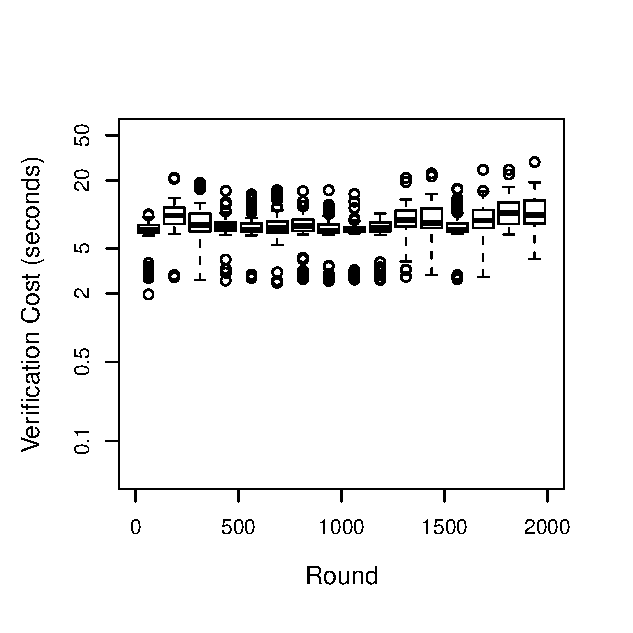
\epsfig{file=figures/tissec/xpilot_lazy_vanilla_time_box_uniform_scale.eps, width=\figurewidth}}
&
\subfigure[][{\parbox[t]{1.15in}{Cost per round (\lazy) with \xpilot-specific optimizations}}]{
	\label{fig:xpilottime:lazyopt}
	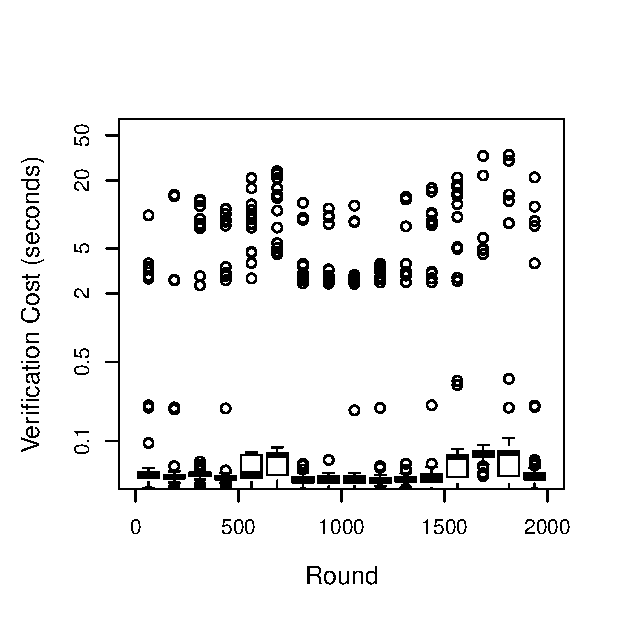
\epsfig{file=figures/tissec/xpilot_lazy_time_box_uniform_scale.eps, width=\figurewidth}}
&
\subfigure[][{\parbox[t]{1.15in}{Cost per round (\eager) with \xpilot-specific optimizations}}]{
	\label{fig:xpilottime:eageropt}
	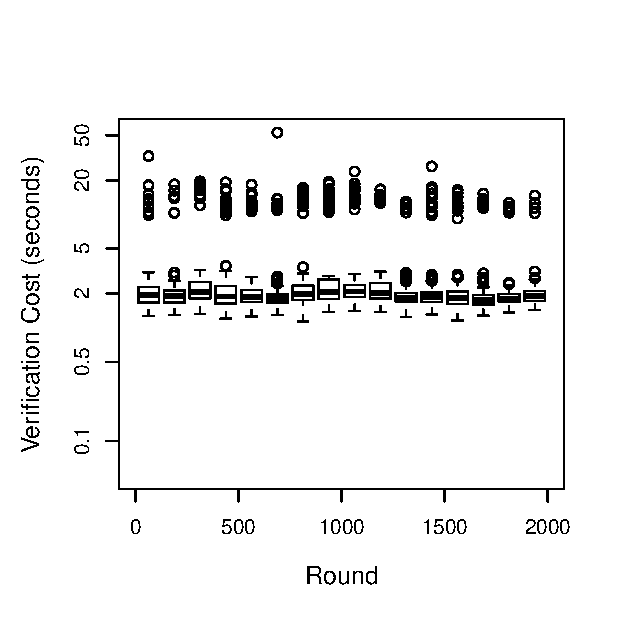
\epsfig{file=figures/tissec/xpilot_eager_time_box_uniform_scale.eps, width=\figurewidth}}
\end{tabular}
\caption{Verification cost per round while checking a 2,000-round
\xpilot game log \label{fig:xpilottime}}
\end{figure*}

By employing an \xpilot-specific optimization, we were able
to significantly improve verification performance.  After the trimming
described in \secref{ssec:scv:xpilot:mods}, the user input paths that we
included within our symbolic execution of the client each caused
another client-to-server message to be sent, and so the number of such
sends in a round indicates to the \verifier an upper bound on the
number of user inputs in that round.  As such, we could tune the
\verifier's symbolic execution to explore only paths through the
client where the number of invocations of the input-handling function
equals the number of client messages for this round in the log.  This
optimization yields the graph in Figure~\ref{fig:xpilottime:lazyopt}.
Notice that there are three distinct bands in the graph, corresponding
to how many times the input-handling function within the game client
was called.  The first band contains rounds which called the input
handler zero times and represents the majority (90.1\%) of the total
rounds.  These rounds were the quickest to process, with a mean cost
of 53.8ms and a standard deviation of 21.1ms.  The next-largest band
(5.1\%) contains rounds which called the input handler only once.
These rounds took longer to process, with a mean of 3.26s and a
standard deviation of 1.05s.  The final band represents rounds with
more than one call to the input-handling function.  This band took the
longest to process (12.9s, on average), but it was also the smallest, 
representing only 4.1\% of all rounds.

\subsection{Verification with \Eager \PathsegCons}
\label{ssec:scv:xpilot:eager}

In this section we discuss verification of \xpilot using \eager
constraint generation.  Recall that \eager \pathsegcons are
precomputed from the sanctioned client software without knowledge of
the messages the client will process in any given loop iteration.
However, we found this approach to require moderate manual tuning
to be practical, as we describe below.

\subsubsection{Manual Tuning}
\label{sssec:xpilot:eager:tuning}

A direct application of our method for generating \eager
\pathsegcons for the \xpilot client loop would replace the user key
press with symbolic input and any incoming server message with a
symbolic buffer and then use \klee to symbolically execute the
resulting client program.  Such a direct application, however,
encountered several difficulties.  In this section we describe the
main difficulties we encountered in this direct approach and the
primary adaptations that we made in order to apply it to the \xpilot
client.  These adaptations highlight an important lesson: the \eager
technique, while largely automatic, can require some manual tuning to
be practical.  Because our technique is targeted toward game
developers, we believe that allowing for such manual tuning is
appropriate.

\subsubsection{Frame processing}
In \xpilot, messages from the server to the client describing the
current game state are called {\em frames}.  Each frame is formed of a
chain of game {\em packets} (not to be confused with network packets).
The first and last packets in a frame are always special
start-of-frame and end-of-frame packets, called \pktstart and \pktend.
Figure~\ref{fig:xpframe} shows an \xpilot frame, containing a packet
of type \pktfuel and potentially others (indicated by ``$\ldots$'').
Packets are encoded as a single header byte followed by a packet data
section that can carry anything from a single byte to an
arbitrary-length string, depending on the packet type.  Frames may
contain multiple packet types and multiple instances of the same
packet type.

%\begin{wrapfigure}{r}{0.3\textwidth}
\begin{figure}[t]
  \centering
  \begin{tabular}{|c|}
    \hline
    \pktstart header \\[10pt] \hline \pktstart data \\ $\vdots$\\[10pt]
    \hline\hline
    \pktfuel header \\[10pt] \hline \pktfuel data \\$\vdots$\\[10pt]
    \hline\hline
    $\ldots$ \\[10pt]
    \hline\hline
    \pktend header \\[10pt] \hline \pktend data \\$\vdots$\\[10pt]
    \hline
  \end{tabular}
  \caption{\xpilot frame layout}
  \label{fig:xpframe}
\end{figure}
%\end{wrapfigure}

Consider the client's frame-processing algorithm.  Given a frame, it
first reads the packet header (i.e., the first byte), then calls the
handler for that packet, which processes the packet and advances the
frame pointer so that the new ``first byte'' is the packet header of
the next packet in the frame.  This continues until the packet handler
for \pktend is called, the return of which signifies the end of the
frame handling.  Therefore, given a completely symbolic buffer
representing the frame, our symbolic execution would need to walk the
client code for {\em each possible sequence} of packets in a frame, up
to the maximum frame size.  But \xpilot has dozens of packet types,
some of which include a very small amount data.  As evidence of the
infeasibility of such an approach, consider the following (very
conservative) lower bound on the number of packet sequences: There are
at least 10 types of packets that we considered whose total size is at
most 5 bytes.  The maximum size for a server-to-client frame in
\xpilot is 4,096 bytes, which means there is room for over 800 of
these packets.  That gives {\em at least} $10^{800}$ possible packet
sequences that symbolic execution would traverse to generate
constraints, which is obviously infeasible.

To make \eager constraint generation feasible, then, we adapt our
approach to generate \pathsegcons by starting and stopping symbolic
execution at multiple points within the loop, as opposed to just the
beginning and end.  In particular, we apply symbolic
execution to the frame-processing and user input-processing portions
of the loop separately, to obtain {\em \inputcons} and {\em
  \framecons}, which in turn the \verifier pieces together {\em during
  verification} to construct the \pathsegcons.  Moreover, the
\verifier can construct the \framecons on the basis of the particular
frame the server sent to the client.  It does so dynamically from
\packetcons that characterize how the client should process each
packet in the particular frame.  For example, if the only
packet types were \pktstart, \pktfuel, \pkttimeleft, and \pktend, the
\packetcons representing the processing of a single packet would be
\[\begin{array}{l}
( \packettype = \pktstart ) \wedge (\constraintsfor{\pktstart}) \\
( \packettype = \pktfuel ) \wedge (\constraintsfor{\pktfuel}) \\
( \packettype = \pkttimeleft ) \wedge (\constraintsfor{\pkttimeleft}) \\
( \packettype = \pktend ) \wedge (\constraintsfor{\pktend})
\end{array}\]
where \packettype is a variable for the packet type and
\constraintsfor{\pktstart} represents the additional constraints that
would result from symbolic execution of the packet handler for
\pktstart.  With this new model of packet processing, the \verifier
can build a \framecon to represent any given frame from the logs.  In
this way, when the \verifier checks the behavior of a given client, it
does so armed with the frames the server sent to the client, the
messages the server
received from the client, and the \framecons that characterize the
client's processing of each frame, which the \verifier constructs from
the \packetcons.

\subsubsection{Packet processing} Certain individual packet types present
their own tractability challenges as well.  For example, the payload
for a certain packet begins with a 32-bit mask followed by one byte
for each bit in the mask that is equal to 1.  The client then stores
these remaining bytes in a 32-byte array at the offsets determined by
the mask (setting any bytes not included in the message to 0).  In the
packet handler, the \xpilot client code must sample the value of each
bit in the mask in turn.  Since the payload (and thus the mask) is
symbolic, each of these conditionals results in a fork of two separate
paths (for the two possible values of the bit in question).  Our
symbolic execution of this packet handler, then, would produce over 4
billion \pathsegcons, which is again infeasible.  We could have
changed the \xpilot protocol to avoid using the mask, sending 32 bytes
each time, but doing so would increase network bandwidth needlessly.
Instead, we note that the result of this packet handler is that the
destination array is set according to the mask and the rules of the
protocol.  We thus added a simple rule to the \verifier that, when
processing this type of packet, generates a constraint defining the
value of the destination array directly, as the packet handler would
have.  Then, when symbolically executing the packet handlers, we can
simply skip this packet.

To avoid similar modifications to the extent possible, we pruned the
packets the \verifier considers during verification to only those that
are necessary.  That is, there are several packet types that will not
alter the permissible behaviors of the client as could be witnessed by
the server, and so we ignored them when applying our technique.  Most
of these packet types represent purely graphical information.  For
example, a packet of type \pktitem simply reports to the client that a
game item of a given type (e.g., a power-up or a new weapon) is
floating nearby at the given coordinates.  This information allows the
client to draw the item on the screen, but it does not affect the
valid client behaviors as observable by the \verifier.\footnote{In
  particular, whether the client processes this packet is irrelevant
  to determining whether the client can pick up the game item
  described in the packet.  Whether the client obtains the item is
  unilaterally determined {\em by the server} based on it computing
  the client's location using the low-level client events it receives
  --- an example of how nearly all control is stripped from clients in
  today's games, owing to how they cannot be trusted.}

\subsubsection{User input}
The first part of the client input loop checks for and handles input
from the player.  Gathering \inputcons is fairly straightforward, with
the exception that \xpilot allows players to do an extensive amount of
keyboard mapping, including configurations in which multiple keys are
bound to the same function, for example.  We simplified the generation
of constraints by focusing on the user actions themselves rather than
the physical key presses that caused them.  That is, while generating
constraints within the user-input portion of \xpilot, we begin
symbolic execution {\em after} the client code looks up the in-game
action bound to the specific physical key pressed, but {\em before}
the client code processes that action.  For example, if a user has
bound the action \keyfireshot to the key `{\tt a}', our analysis would focus
on the effects of the action \keyfireshot, ignoring the actual key to
which it is bound.  However, as with other client configuration
options, the keyboard mapping could easily be sent to the server as a
requirement of joining the game, invoking a small, one-time bandwidth
cost that would allow the \verifier to check the physical key
configuration.

\subsubsection{\Eager Verification Performance}
\label{sssec:xpilot:eager:eval}

We ran our \eager client verifier on the same 2,000-round \xpilot game
log and on the same computer used in \secref{ssec:scv:xpilot:lazy}.
Figure~\ref{fig:xpilottime:eageropt} describes the per-round
validation cost (in seconds) using a box-and-whiskers plot.  As in
Figure~\ref{fig:xpilottime:lazyopt}, we employed here an
\xpilot-specific optimization by observing that the number of client
messages in a round bounds the number of user inputs in that round.
As such, in piecing together \pathsegcons, the \verifier includes a
number of copies of \inputcons (see \secref{sssec:xpilot:eager:tuning})
equal to the client sends in that round.  Similar to
Figure~\ref{fig:xpilottime:lazyopt},
Figure~\ref{fig:xpilottime:eageropt} exhibits three bands (the third
comprising a few large values), corresponding to different numbers of
copies.  The large percentage of rounds contained no user inputs and
were the quickest to process, with a mean cost of 1.64s and a standard
deviation of 0.232s.  The second band of rounds --- those with a
single user input --- took longer to process, with a mean of 11.3s and
a standard deviation of 1.68s.  Remaining rounds contained multiple
user inputs and took the longest to process (34.2s, on average), but
recall that they were by far the least frequent.  The \verifier's
memory usage remained below 100MB throughout these verification runs.

Comparing
Figures~\ref{fig:xpilottime:lazyopt} and~\ref{fig:xpilottime:eageropt},
the times for the \eager approach are much slower than those
for the \lazy approach, when applied to \xpilot.  This performance
loss is due to the fact that a large portion of the \xpilot client
code is dedicated to handling server messages.  And while the
\verifier in the \eager case has preprocessed this portion of the
code, the resulting \pathsegcons are much more complex than in the
\lazy approach, where the \verifier knows the exact values of the
server messages when generating \pathsegcons.  This complexity results
in constraint solving in the \eager case
(line~\ref{fig:trackConstraints:isSat} of
Figure~\ref{fig:trackConstraints}) being more expensive.

It is also important to recall that \lazy and \eager are not
interchangeable, at least in terms of game developer effort.  As
discussed in \secref{sssec:xpilot:eager:tuning}, achieving feasible
generation of \eager \pathsegcons required substantial additional
manual tuning, and consequently greater opportunity for programmer
error.  As such, it appears that the \eager approach is inferior to
the \lazy approach for \xpilot.  Another comparison between the two
approaches, with differing results, will be given in
\secref{sec:scv:capman}.

\section{Case Study: \capman}
\label{sec:scv:capman}

Our client verification technique challenges the current game-design
philosophy by allowing servers to relinquish authoritative state to
clients while retaining the ability to validate client behavior and
thus detect cheating.  As a way of demonstrating this notion, we have
written a game called \capman that is based on the game \pacman.  In
some ways \capman is easier to validate than \xpilot was --- it
represents a considerably smaller code base (roughly 1,000 lines
of C code) and state size.

That said, \capman is interesting as a case study for three reasons.
First, whereas \xpilot was written with virtually no authoritative
client state, we will see that \capman is intentionally rife with it,
providing a more interesting challenge for our technique because it is
so much more vulnerable to invalid messages.  Second, the size of its
code base allows us to conduct a more direct comparison between \lazy
and \eager verification.  Third, \capman differs from \xpilot in that
the set of possible user inputs per round is substantially larger than
the set of paths through the client's event loop.  That is, in
\xpilot, there is nearly a one-to-one correspondence between user
inputs and paths through the client event loop, which dampens the
improvement that our technique offers over, e.g., the \verifier simply
running the client on all possible inputs in each round.  \capman
demonstrates the scalability of our technique to many possible user
inputs when this is not the case, thereby separating our technique
from other such possible approaches.

\subsection{The Game}

\capman is a \pacman-like game in which a player controls an avatar
that is allowed to move through a discrete, two-dimensional map with
the aim of consuming all remaining ``food'' items before being caught
by the various enemies (who are also navigating the map).  Each map
location is either an impenetrable wall or an open space, and the open
spaces can contain an avatar, an enemy, pieces of food, a power-up, or
nothing at all.  When a player reaches a map location that contains
food or a power-up, he automatically consumes it.  Upon consuming a
power-up, the player enters a temporary ``power-up mode,'' during
which his pursuers reverse course --- trying to escape rather than
pursue him --- and he is able to consume (and temporarily displace)
them if he can catch them.  In addition to these features (which were
present in \pacman as well), we have added a new feature to \capman to
invite further abuse and create more uncertainty at the server: A
player may set a bomb (at his current location), which will then
detonate a number rounds in the future selected by the user from a
predefined range (in our implementation, between 3 and 15
rounds).\footnote{In our preliminary work~\cite{bethea10:games}, a
  bomb detonated in a fixed number of rounds.  We changed the game to
  accommodate a user-selected number of rounds to bomb detonation in
  order to demonstrate the ability of our technique to scale to a
  larger number of possible user inputs.}  When it detonates, it kills
any enemies (or the player himself) within a certain radius on the
map.  Players are not allowed to set a new bomb until their previous
bomb has detonated.

\capman uses a client-server architecture, which we designed
specifically to go against current game-development best practices:
i.e., it is the {\em server}, not the client, which has a minimum of
authoritative state.  The client tracks his own map position,
power-up-mode time remaining, and bomb-placement details.
Specifically, at every round, the client sends a message to the server
indicating its current map position and remaining time in power-up
mode.  It also sends the position of a bomb explosion, if there was
one during that round.  Note that the client never informs the server
when it decides to {\em set} a bomb.  It merely announces when and
where detonation has occurred.  The server, in contrast, sends the
client the updated positions of his enemies --- this being the only
game state for which the server has the authoritative copy.

The design of \capman leaves it intentionally vulnerable to a host of
invalid-message attacks.  For example, although valid game clients
allow only contiguous paths through the map, a cheating player can
arbitrarily adjust his coordinates, ignoring the rules of the game ---
a cheat known in game-security parlance as ``telehacking.''  He might
also put himself into power-up mode at will, without bothering to
actually consume a power-up.  Finally, there is no check at the server
to see whether or not a player is lying about a bomb placement by, for
example, announcing an explosion at coordinates that he had not
actually occupied within the past 15 rounds.  In fact, the \capman
server contains no information about (or manual checks regarding) the
internal logic of the game client.

In order to detect cheating in \capman, we apply our technique in both
its \lazy and \eager variations.  Due to \capman's smaller size and
simpler code structure, we can generate \pathsegcons over an entire
iteration of the main loop in each case, without the need to
compartmentalize the code and adopt significant trimming measures as
we did for \xpilot.

\subsection{Evaluation}

Using our technique, we are able to detect invalid-command cheats of
all the types listed above.  Below we present the results of
client-validity checks on a game log consisting of 2,000 rounds (about
6-7 minutes of game-play time), during which the player moved around the
map randomly, performing (legal) bomb placements at random intervals.

\begin{figure*}[t]
\hspace{-5pt}
\begin{tabular}{@{\extracolsep{-1.25em}}ccc}
\subfigure[][{\parbox[t]{1.1in}{Cost per round (\lazy)}}]{
	\label{fig:capmantimes:lazy}
	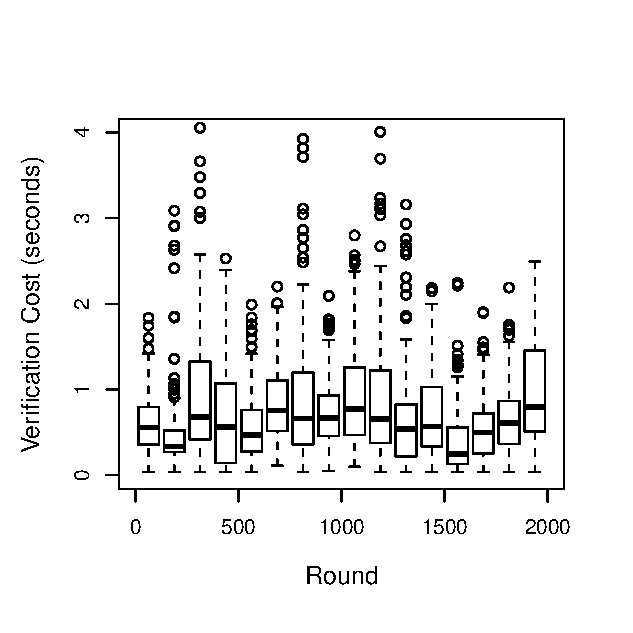
\epsfig{file=figures/tissec/capman_lazy_time_box.eps, width=\figurewidth}}
&
\subfigure[][{\parbox[t]{1.15in}{Cost per round (\eager)}}]{
	\label{fig:capmantimes:eager}
	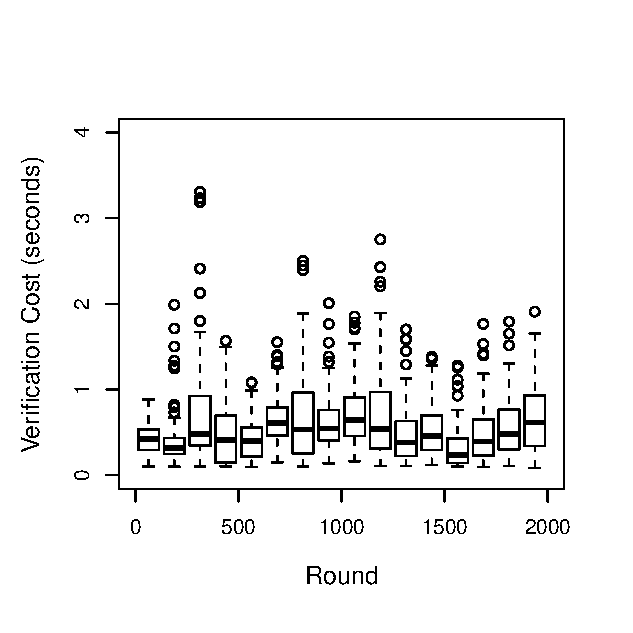
\epsfig{file=figures/tissec/capman_eager_time_box.eps, width=\figurewidth}}
&
\subfigure[][{\parbox[t]{1.5in}{Satisfiable \execpathcons per round (\eager)}}]{
	\label{fig:capmanchainsplot}
	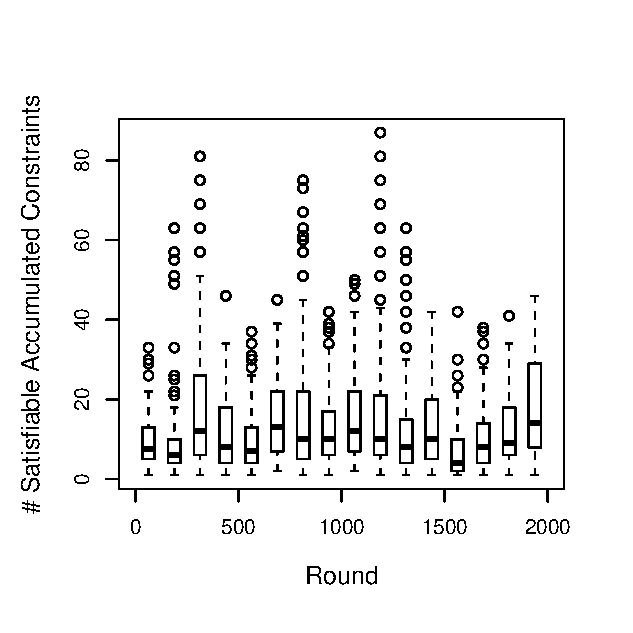
\epsfig{file=figures/tissec/capman_eager_chains_box.eps, width=\figurewidth}}
\end{tabular}
\caption{Verifying a 2,000-round \capman game log}
\label{fig:capmantimes}
\end{figure*}

Figure~\ref{fig:capmantimes} shows that the verification costs for
\capman were consistently small, with a mean and standard deviation of
752ms and 645ms for verification via \lazy \pathsegcons
(Figure~\ref{fig:capmantimes:lazy}) and a mean and standard deviation
of 310ms and 193ms for verification using \eager \pathsegcons
(Figure~\ref{fig:capmantimes:eager}).  The \lazy method was (on
average) roughly 2.5 times slower than the \eager method, owing to the
overhead of symbolic execution to compute \pathsegcons for each round
individually during verification.  The \verifier's memory usage
remained below 100MB throughout verification of both types.  While in
the \xpilot case study, \eager verification required significantly
greater development effort (see \secref{sssec:xpilot:eager:tuning}),
this additional effort was unnecessary with \capman due to its
relative simplicity.

Figure~\ref{fig:capmanchainsplot} shows the number of satisfiable
\execpathcons during \eager verification, which did not trend upward
during the run.  In \lazy verification, the number of satisfiable
\execpathcons was virtually identical.  (Variations in our pruning
implementations caused less than $1\%$ of the rounds to differ, and
then by at most 12 \execpathcons.) In the case of \xpilot, the number
of satisfiable \execpathcons was always $1$, but in \capman there were
often multiple \execpathcons that remained satisfiable at any given
round.  This increase resulted primarily from state the \capman client
maintains but does not immediately report to the server (e.g., whether
a bomb has been set, and with what detonation timer).  The
relationship between this hidden state and the number of satisfiable
\execpathcons is an important one.  Consider the verification of a
\capman game that is currently in round $\roundidx$, with no bomb
placements in the last 15 rounds (unbeknownst to the \verifier).  The
\verifier must maintain \execpathcons that reflect possible bomb
placements at each of rounds $\roundidx-14$ through $\roundidx$.  Upon
encountering $\clientMsg_{\roundidx+1}$ with an announcement of a bomb
explosion, the \verifier can discard not only all current
\execpathcons which do {\em not} include a bomb placement in any of
rounds $\roundidx-14$ through $\roundidx-2$, but also those
\execpathcons which {\em do} include bomb placements in rounds
$\roundidx-1$ through $\roundidx+1$, because players can only have one
pending bomb at a time.  This rule was not manually configured into
the \verifier; it was inferred automatically from the client code.

\section{Case Study: \tetrinet}
\label{sec:scv:bandwidth}

As discussed earlier, our verification technique
presents opportunities to reduce the bandwidth consumed by an online
game, since it allows the client's management of state to be verified
with less-than-complete information.
In our third case study, we used a pre-existing game called \tetrinet
in order to explore simple bandwidth-savings measures and their impact
on client verification performance.

\subsection{The Game}
\tetrinet is a multiplayer clone of the classic puzzle game \tetris.
It was originally developed in 1997 but remains popular and has been
reimplemented on many different platforms.  In the game, random
\textit{tetrominoes}, which are geometric shapes consisting of four
connected blocks, automatically advance down each player's playing
field, one at a time.  As each does, the player can rotate it into
four possible orientations or slide it horizontally left or right.
The objective of the game is to arrange tetrominoes so that, as they
land, they create gapless horizontal rows of blocks on the playing
field.  When such a gapless row is created, it is cleared, each row of
blocks above it falls down one row, and --- in the primary multiplayer
departure from \tetris{} --- a line with gaps is added to the bottom
of the other players' fields.  A player loses when there is no room
for an additional tetromino to enter her playing field.  \tetrinet is
implemented in C and has a client-server architecture similar to
\capman and \xpilot.  The server does virtually no checking on client
messages and so is vulnerable to cheats; e.g., a client could indicate
it cleared a row that has gaps or placed a new tetromino in a spot
that the client should not have allowed it to reach.

Enabling the use of our verification tool with \tetrinet required some
consideration of how the user input operates. A tetromino in play
automatically moves down one row every $0.5$~seconds, and when the
piece can move no further, the position is fixed and a new random
piece starts falling from the top of the game screen. The placement of
the tetromino in a permanent resting point defines the end of single
round of gameplay, at which time the \tetrinetHorizontal and
\tetrinetVertical coordinates and the rotation \tetrinetOrientation
are sent to the server. Until the end of the round, though, the player
can move the piece horizontally or rotate it as many times as she
wishes. So, even though there is a finite number of final fixed
positions for a game piece in a given round, there are theoretically
an infinite number of possible inputs sequences that could lead to
each valid final position. To minimize the number of input sequences
that must be explored symbolically, we considered a restricted version
of gameplay where the gameboard must be empty above each tetrimino at
the time of its placement, and so three rotations and six horizontal
moves sufficed to reach any such placement on the 12-column gameboard.

\subsection{Evaluation}
To demonstrate bandwidth reduction in \tetrinet using our verification
technique, we simply reduced the information in the client-to-server
messages. \tetrinet was modified so that only every
\tetrinetUnabridgedFreq rounds was the complete tuple
$(\tetrinetHorizontal, \tetrinetVertical, \tetrinetOrientation)$ sent
to the server (an ``unabridged message'').  In other rounds, the
client sent a partial tuple, omitting \tetrinetHorizontal,
\tetrinetVertical, or \tetrinetOrientation or both \tetrinetVertical
and \tetrinetOrientation.  Figure~\ref{fig:tetrinettimes} shows the
tradeoff between the bandwidth reductions accomplished and the costs
of verifying client behavior using the \lazy client verifier, where
the bandwidth reductions were calculated assuming \tetrinetHorizontal,
\tetrinetVertical and \tetrinetOrientation are sent in four, five, and
two bits, respectively.  (The actual \tetrinet implementation is not
engineered for bandwidth reduction and so uses payload space more
wastefully.)  These graphs each represent five random play sessions of
100 rounds each and the same five play sessions were used for each of
the four experiments.  Note that $\tetrinetUnabridgedFreq=1$ is
equivalent to verification of an unmodified game client. In the
experiment where \tetrinetVertical is omitted, the verification cost
does not increase because there is no ambiguity as to
\tetrinetVertical's value when \tetrinetHorizontal and
\tetrinetOrientation are provided. During these verification runs,
the \verifier's memory usage remained below 512MB.

\begin{figure}[t]
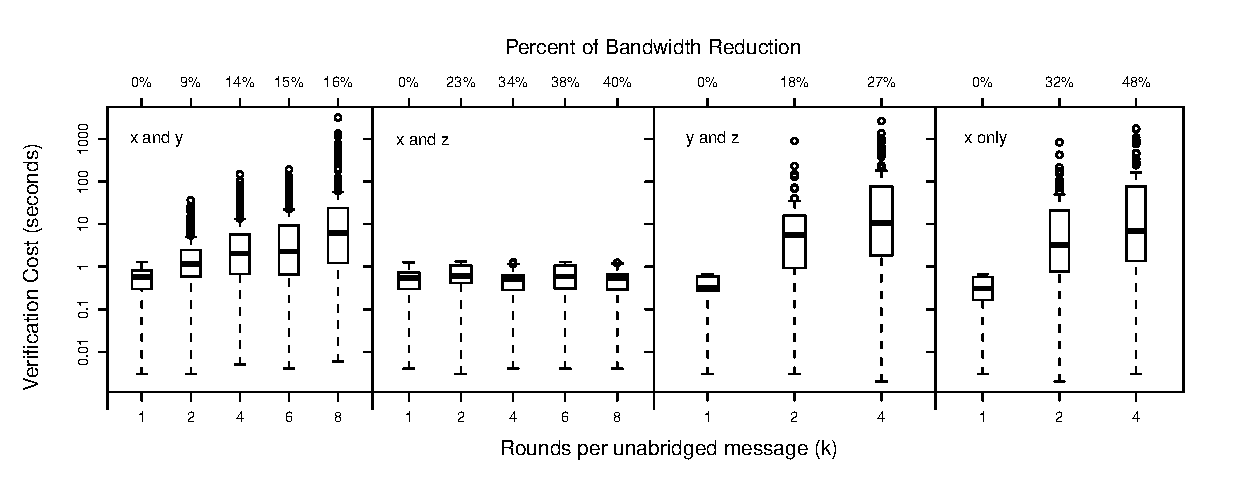
\epsfig{file=figures/tissec/tetrinet_time_vs_bandwidth_grid.eps, width=\textwidth}
\caption{Verification of 100-round \tetrinet logs under different
configurations of client-to-server message content.}
\label{fig:tetrinettimes}
\end{figure}

\section{Verification with message loss}
\label{sec:scv:message-loss}

Games today must be built to tolerate a range of networking
conditions, including occasional message loss.  While there are
standard approaches to recovering lost messages, such as message
retransmission at the transport level (i.e., using TCP) or at the
application level, retransmission is avoided in some games for two
reasons.  First, the importance of some messages diminishes quickly,
and so by the time the message would be retransmitted, the utility of
doing so is lost.  Second, retransmission can introduce overheads that
high-performance games cannot tolerate.


Lost server-to-client messages pose little difficulty to our client
verification technique; all the \verifier requires is to know what
server-to-client messages the client processed and when, which can be
communicated from the client efficiently (e.g., see
\secref{app:acks}).  Lost client-to-server messages pose more
difficulty, however.  Intuitively, our technique can handle client
message loss by instantiating the constraint \msgConstraint for a
missing round-\roundidx message $\clientMsg_{\roundidx}$ to simply
$\msgConstraint = ``\mathrm{true}"$ in
Figure~\ref{fig:trackConstraints}.  However, this has two negative
consequences.

First, from the server's (and \verifier's) perspective, it is
impossible to distinguish a lost message from one the client only
pretended to send.  This can be used by a cheating client to gain
latitude in terms of the behaviors that the \verifier will consider
legitimate.  For example, whenever a power-up appears on the game map,
an altered game client could collect it by reporting its player's
position at the power-up's location.  So as to not be caught by the
\verifier, the client could alter its state to reflect having sent
messages that would have been induced by the player actually moving to
that location, even though these messages were never sent and so, from
the server's perspective, were lost. Because it is possible for a
valid client on a poor network connection to generate
indistinguishable behavior, this cheat is not in the class that our
\verifier detects. Nevertheless, as discussed in
\chref{ch:background},
our techniques are compatible with existing methods that address this
type of cheat.

Another consequence of message loss is that the performance of
verification can be severely impacted by it.  The performance results
in \secref{sec:scv:xpilot}--\ref{sec:scv:capman} did not reflect the loss of
any client messages; instead, the game logs that we validated included
all messages that the client sent.  However, in practice message loss
causes the \execpathcons $\execPathConstraints_{\roundidx}$
to grow dramatically, since {\em any} path through the client that
causes a message to be sent is deemed possible in round \roundidx.  As
a result, in experimenting with message loss in \xpilot, we found that
in the face of lost messages, the performance of our technique decays
very substantially.

As such, we propose a lightweight scheme to enable our technique to
retain its performance in the face of (limited) message loss.  Rather
than retransmitting messages, our technique communicates a small
amount of additional information per client-to-server message to
enable the \verifier to prune \execpathcons effectively in the face of
message loss.  Intuitively, the client remembers the path through its
event loop that it traverses in round \roundidx and then conveys
evidence of this to the server over the next several messages.  The
server records this evidence for the \verifier, which uses it to prune
\pathsegcons considered for round \roundidx.

There are several ways to instantiate this intuition within our
framework.  Here we describe one implementation that works well in
\xpilot.  In this implementation, the ``evidence'' that the client
conveys to the server for the path it traversed in round
\roundidx is a hash of the fields of the message it sent in round
\roundidx that are a function of (only) the path traversed.
Rather than send the entire hash in a subsequent message, however, the
client ``trickles'' this hash value to the server, e.g., one bit per
message, so that subsequent message losses still enable the server to
collect a number of hash bits for each round.  After the client's
messages are recorded at the server, the \verifier collects these bits
and uses them to prune the \pathsegcons considered at each step of
verification where it is missing a message.

We have prototyped this approach in the context of \lazy verification,
in order to validate the ability of the \xpilot \verifier to retain
its performance in the face of message losses.  (\capman and \tetrinet
use TCP and so do not face message-loss issues.)  The hash we use is a
\hashsize-bit BSD \texttt{sum}, and the \bitidx-th bit of the
round-\roundidx message hash is carried on the round
$\roundidx+\bitidx$ message ($1 \le \bitidx \le \hashsize$).  As such,
each message carries an extra \hashsize bits composed of bits from the
previous \hashsize client-to-server messages.

%\begin{wrapfigure}{r}{0.35\textwidth}
\begin{figure}[t]
\centering
%\vspace{-0.2in}
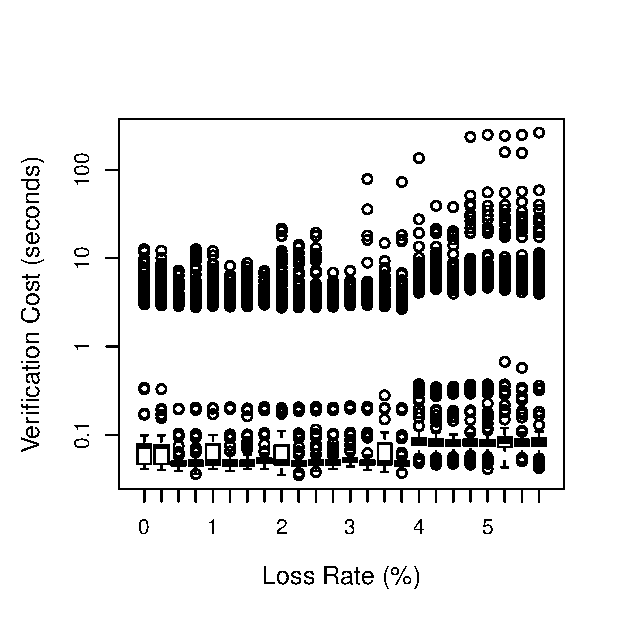
\epsfig{file=figures/tissec/xpilot_lazy_lossrates_box.eps, width=\figurewidth}
%\vspace{-0.1in}
\caption{Verification (\lazy) of 2000-round \xpilot log with loss of
client-to-server messages at the rate indicated on horizontal axis.}
\label{fig:random_loss} 
%\vspace{-0.1in}
%\end{wrapfigure}
\end{figure}

To show the effectiveness of this approach, we repeated the
\lazy verification of $2000$-round \xpilot game logs using \xpilot-specific
optimizations (c.f., Figure~\ref{fig:xpilottime:lazyopt}) but
introduced client-to-server message losses to show that our approach
tolerates them seamlessly.  We experimented with two types of message
loss.  In the first, each client-to-server message is lost with a
fixed probability.  Figure~\ref{fig:random_loss} shows
box-and-whiskers plots that illustrate the per-round verification
costs that resulted, as a function of this loss rate.  Note that a
message loss rate of 4\% earns a ``critical'' designation at a
real-time monitoring site like \url{www.internetpulse.net}.  As
Figure~\ref{fig:random_loss} shows our technique can easily handle
such a high loss rate.

A second type of loss with which we experimented is a burst loss,
i.e., the loss of a contiguous sequence of client-to-server messages.
Figure~\ref{fig:burst_loss} shows the verification costs per round in
five different message logs in which a burst loss of length $6$, $10$,
or $14$ client-to-server messages is introduced at a random point
between the $100$th and $150$th round.  As these graphs show, the
verification costs do tend to spike in the region where the burst loss
occurs, but the verification costs remain feasible and recover after
the burst to their original durations.  Only when the burst length
exceeds \hashsize (not shown) do the verification costs become and
remain too large to be practical.

%\clearpage
\begin{figure}[ht]
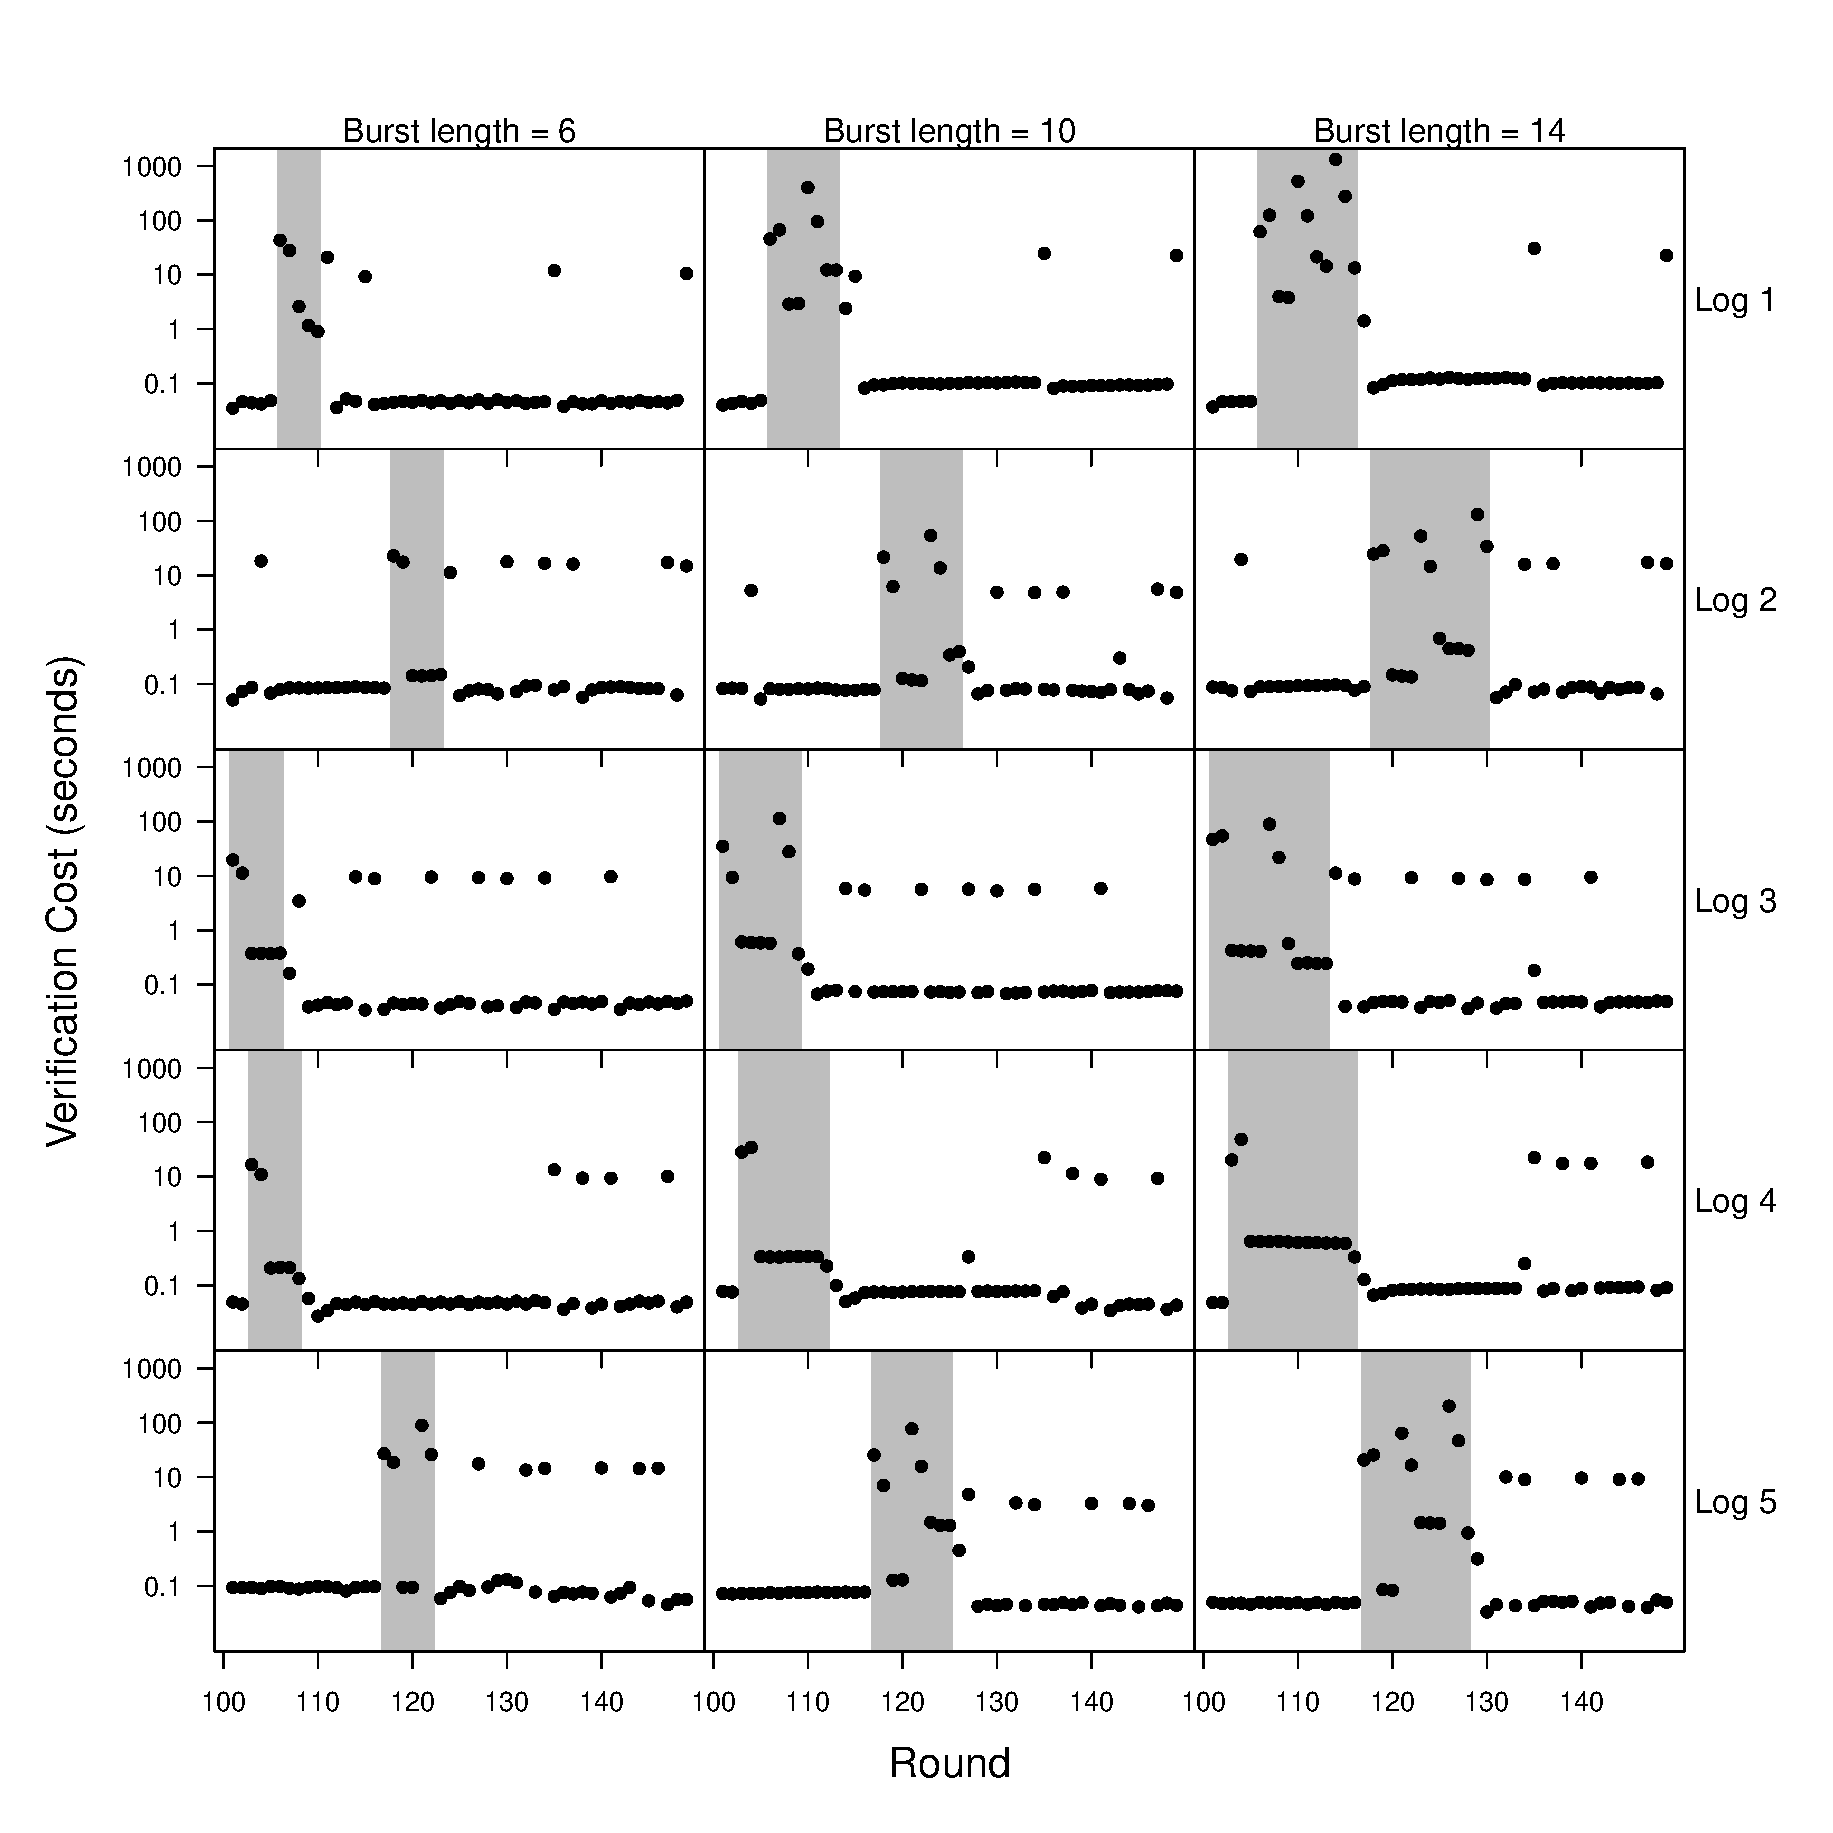
\epsfig{file=figures/tissec/xpilot_lazy_burstsize_grid.eps, width=\textwidth}
\caption{Verification (\lazy) of \xpilot logs with randomly induced
bursts of client-to-server message losses.  Shaded areas designate
rounds in which losses occurred.}
\label{fig:burst_loss}
\end{figure}
\clearpage

%\subsection*{Acknowledgements}
%
%We are deeply grateful to Cristian Cadar, Daniel Dunbar, and Dawson
%Engler for helpful discussions and for permitting us access to an
%early release of \klee.  Srinivas Krishnan, Alana Libonati, Andy White
%and the anonymous reviewers provided helpful comments on drafts of
%this paper.  This work was supported in part by NSF awards 0756998,
%0910483, and 1115948.

\section{Acknowledgement Scheme for \xpilot}
\label{app:acks}

As discussed in \secref{ssec:scv:xpilot:mods}, an efficient acknowledgement
scheme allows the server (and hence \verifier) knowledge of the order
(and loop iterations) in which the client processed server messages
and sent its own messages.  Below we describe one such scheme that is
optimized for messages that arrive at the client mostly in order.

In this scheme, the \xpilot client includes a sequence number \cToSNbr
on each message it sends to the server, and similarly the server
includes a sequence number \sToCNbr on each message it sends to the
client.  Each message from the server to a client also includes the
largest value of \cToSNbr received from that client.  In each client
message, the client includes \cToSAckd, the largest value of \cToSNbr
received in a server message so far; a sequence \lateMsgs{} of server
message sequence numbers; and a sequence \symbSeq{} of symbols that
encode events in the order they happened at the client.  The symbols
in \symbSeq{} can be any of the following.  Below, \sToCAckd is the
largest sequence number \sToCNbr received by the client before sending
message \cToSAckd, and similarly \loopAckd is the largest client loop iteration
completed at the client prior to it sending \cToSAckd.

\begin{itemize}
\item \symbLoop denotes a completed loop iteration.  The $\symbLoopCtr$-th
occurrence of \symbLoop in \symbSeq{} denotes the completion of loop
iteration $\loopAckd + \symbLoopCtr$.
\item \symbSent denotes the sending of a message to the server.  The
$\symbSentCtr$-th occurrence of \symbSent in \symbSeq{} denotes the
sending of client message $\cToSAckd+\symbSentCtr$.
\item \symbRcvd and \symbSkip denote receiving or skipping the
next server message in sequence.  The $\symbRorSCtr$-th occurrence of
\symbRcvd or \symbSkip in \symbSeq{} denotes receiving or skipping,
respectively, server message $\sToCAckd+\symbRorSCtr$.  Here, a
message a skipped if it has not arrived by the time a server message
with a larger sequence number arrives, and so a series of one or more
\symbSkip symbols is followed only by \symbRcvd in \symbSeq{}.
\item \symbLate denotes the late arrival of a message, i.e., the
arrival of a message that was previously skipped.  The
$\symbLateCtr$-th occurrence of \symbLate in \symbSeq{} denotes the
arrival of server message \lateMsgs{\symbLateCtr}.
\end{itemize}

As such, \lateMsgs{} contains a sequence number for each server
message that arrives after another with a larger sequence number, and
so \lateMsgs{} should be small.  \symbSeq{} may contain more elements,
but the symbols can be encoded efficiently, e.g., using Huffman
coding~\cite{huffman52:codes}, and in at most three bits per symbol in
the worst case.  Note that the server can determine \sToCAckd and
\loopAckd based on the previous messages received from the client.

\section{Summary}
\label{sec:scv:conclusion}

%The need to detect cheats has heavily influenced the design of online
%games.  Cheating has driven game developers to minimize or eliminate
%authoritative state from game clients.  These measures have direct
%impact on the game operator's bottom line, due to the inflated
%bandwidth costs that result and to the manual and heuristic (and hence
%ongoing) effort of programming server-side checks on client behaviors.

In this chapter, we described an approach to validate the server-visible
behavior of remote clients.  Our approach validates that client
behavior is a subset of the behaviors that would be witnessed from the
sanctioned client software, in light of the previous behaviors of the
client and the messages sent to that client.  Our technique exploits
a common structure in clients, namely a loop that accepts server
and user inputs, manages client state, and updates the server with
necessary information.  Our technique
applies symbolic execution to this loop to produce constraints that
describe its effects.  The server operator can then automatically check
the consistency of client updates with these constraints offline.  We
explored both \lazy and \eager approaches to constraint generation and
investigated the programmer effort each entails, as well as their
performance.

We demonstrated our technique in the context of online games with 
three case studies.
In the first, we applied our validation approach to \xpilot, an
existing open-source game.  We detailed the ways we adapted our
technique, in both the \lazy and \eager variants, to allow for
efficient constraint generation and server-side checking.  While this
effort demonstrated applying our approach to a real game, it was less
satisfying as a test for our technique, in that \xpilot was developed
in the mold of modern games --- with virtually no authoritative state
at the client.  We thus also applied our technique to a simple game of
our own design that illustrated the strengths of our technique more
clearly.  We then showed simple ways to leverage our technique to
reduce bandwidth consumption in a game called \tetrinet, and returned
to \xpilot to demonstrate a strategy for dealing with message loss.

%We believe that our technique can change how game developers address
%an important class of game cheats today, and in doing so opens up new
%avenues of game design that permit lower bandwidth utilization and
%better performance.




%\begin{abstract}
%Existing techniques for a server to verify the correctness of client
%behavior in a distributed application suffer from imprecision,
%increased bandwidth consumption, or significant computational expense.
%We present a novel method for a server to efficiently search for a
%code path through the client that ``explains'' each client message,
%even though the server does not know local inputs to the client that
%might have caused the message.  This method gives rise to a precise
%client verification technique that consumes no additional bandwidth
%and that validates most legitimate client messages much faster than
%previous such techniques.  Our technique can gain even further
%improvements with a minimal increase in bandwidth use.  We detail this
%innovation and use it to verify client behavior in two client-server
%games, namely \xpilot and \tetrinet.  In our best configuration,
%verification often keeps pace with \tetrinet gameplay.
%\end{abstract}

\chapter{Guided Client Verification}
\label{ch:guided}

\ignore{
\section{Introduction}
\label{sec:guided:intro}

In client-server applications, client misbehavior can pose dangers to
the larger distributed application in a variety of ways.  A
manipulated client may be able to compromise the server directly if
the server has an extant vulnerability.  Even if the server has no
such vulnerabilities, any application state for which the client is
authoritative can be altered by a misbehaving client and then
propagated via the server to the larger distributed application.

A common approach to defend against client misbehavior is for the
server to validate client messages using a model of valid client
behavior derived from the sanctioned client software.  For example,
Giffin et al.~\cite{giffin02:remote} and Guha et
al.~\cite{guha09:ajax} developed methods to confirm that requests are
consistent with a control-flow model of the client.  This approach
admits false negatives, however --- compromised clients that make
calls consistent with their control-flow models (but that may still
manipulate application state) can escape detection, in a manner
analogous to mimicry attacks on intrusion-detection
systems~\cite{wagner02:mimicry,tan03:hiding}.  Greater precision has
been achieved, but with greater expense.  For example, the \ripley
system~\cite{vikram09:ripley} replays each client on the server in
order to validate the client's requests, but this incurs the bandwidth
overhead of transmitting all client-side inputs (user inputs, timer
values, etc.) to the server to
permit replay and the computational overhead of replaying the client
on the server side.  An approach by Bethea et
al.~\cite{bethea11:games} omits transmitting client-side inputs, thus
not incurring bandwidth overheads, but then must search for whether
there exist inputs that could have produced the client messages
observed at the server.  The resulting computational expense renders
this method of verification useful primarily in an offline fashion
and, even then, only after modifying test applications to constrain
the search spaces they present.
}

In this chapter we develop a client-checking algorithm that retains
precision while permitting better tradeoffs between bandwidth costs
and computational expense in the common case of a legitimate client.
Our algorithm builds from the approach of 
\chref{ch:scv} but makes use of a training phase to guide a
search for a path through the client program that could have produced
a message observed at the server.  One configuration of our algorithm
incurs no additional bandwidth costs, like the approach in
\chref{ch:scv}, but
completes verification much more efficiently in the common case of a
legitimate client.  Another configuration of our algorithm consumes
minimal additional bandwidth --- in our tests, at most two bytes per
client-to-server message --- and completes verification even faster in
the common case of a legitimate client.  Moreover, we reiterate that
our algorithm is precise in the sense of having no false negatives and
no false positives.  That is, any sequence of client messages that our
technique declares legitimate actually is, in the sense that there
exist inputs that would have driven the sanctioned client software to
send that sequence of messages,\footnote{More precisely, the only
source of false negatives is the fidelity of modeling values returned
by components with which the client software interacts (e.g., the
client OS).  This will be discussed further in \secref{sec:guided:eval}.} and
any sequence of client messages that our technique declares impossible
is actually inconsistent with the client software.

To definitively conclude that a sequence of client messages is
impossible (the uncommon case), our algorithm incurs a cost similar to
the technique in \chref{ch:scv}.  As such, we expect
our algorithm to be useful primarily as an data reduction
technique that prunes the client messages that must be logged for
offline analysis by that (or another) technique.  In addition, clients
whose messages are not verified quickly by our technique can be
serviced only provisionally (e.g., with fewer privileges and/or
logging to enable undoing their effects) while their verification is
completed offline.

We evaluate our algorithm in the context of online games.  Online
games provide a useful proving ground for our techniques due to the
frequent manipulation of game clients for the purposes of
cheating~\cite{yan05:classification,lyhyaoui05:categorization,webb08:survey}
and due to the pressure that game developers face to minimize the
bandwidth consumed by their games~\cite{mulligan03:guide}.
%As such,
%our techniques are directly useful for cheat detection in this domain.
%Moreover, Hoglund and McGraw~\cite{hoglund07:games} argue that ``games
%are a harbinger of software security issues to come,'' suggesting that
%defenses against game cheats and game-related security problems will
%be important techniques for securing future massive distributed
%systems of other types. 
Our evaluations show, for example, that
verifying the behavior of a valid client in the \tetrinet game can
often keep up with the pace of gameplay.  Moreover, our algorithm
succeeds in verifying legitimate messages traces of the highly interactive
\xpilot game without game restrictions required in \chref{ch:scv}.

The technique that we develop here is an extension of the technique
presented in \chref{ch:scv} and as such, is also an application of
symbolic execution~\cite{boyer75:select}. Dynamic analysis techniques
like symbolic execution typically face scaling challenges as code
complexity and execution length grow, and our case is no exception.
We believe that the technique we develop here to prioritize path
analysis on the basis of historical usage may be more broadly useful,
i.e., outside of behavior verification in distributed systems, to
contain the expense of dynamic analysis.

%The technique that we develop here is an application of symbolic
%execution~\cite{boyer75:select}, which has been widely studied and
%applied for various purposes (see \secref{sec:guided:related}).  Dynamic
%analysis techniques like symbolic execution typically face scaling
%challenges as code complexity and execution length grow, and our case
%is no exception.  We believe that the technique we develop here to
%prioritize path analysis on the basis of historical usage may be more
%broadly useful, i.e., outside of behavior verification in distributed
%systems, to contain the expense of dynamic analysis.

The rest of this chapter is structured as follows.  We discuss
necessary background in \secref{sec:guided:goals}, and present our algorithm
in \secref{sec:guided:training} and \secref{sec:guided:verification}.  Evaluation
results for this algorithm are presented in \secref{sec:guided:eval}, and we
conclude in \secref{sec:guided:conclusion}.

\ignore{
\section{Related Work}
\label{sec:guided:related}

As we will see, the approach that we take to the behavior
verification problem that we study is an application of symbolic
execution~\cite{boyer75:select}, a dynamic analysis technique that
``executes'' a program with some values unspecified or ``symbolic'',
in order to derive the postconditions of the software on the symbolic
state.  In our case, we symbolically execute the client software with
client-side inputs unknown to the server marked symbolic and then
determine whether the messages received from the client violate the
postconditions derived from the software.  Symbolic execution has a
long history of study in the security and verification communities,
but we believe the optimization problem we study here to be distinct
from prior work, as discussed below.

The applications of symbolic execution that are most related to our
own are in debugging and diagnostics. Zamfir et
al.~\cite{zamfir10:exesyn} developed a debugging tool that uses
symbolic execution to reconstruct the likely path a program took
before it crashed, from the core dump file recorded by the operating
system when the crash occurred.  Their technique finds a feasible path
or set of paths through a program that allow the program to reach the
memory and process state that the core dump file indicates.
\sherlog~\cite{yuan10:sherlog} is another error diagnosis tool that
uses a log file instead of a core dump file to indicate how a program
executed.  \sherlog performs path analysis (not symbolic execution per
se, but a similar technique) to determine the likely execution paths
and variable values implied by a given set of log files.  Similarly,
symbolic execution has been used to discover the constraints for the
paths through a program that reaches a vulnerability or error
condition~\cite{brumley06:vulnsig,caballero09:vulnsig,cadar06:exe,yang06:maldisks}.
Viewed through the lens of this chapter, the core dump file, log file,
or error condition in these previous works is analogous to a ``client
message'', and these tools similarly seek to find an execution that
could explain it.  However, the structure of our verification task ---
namely successively building an execution path to explain an entire
sequence of messages --- and the performance demands that we seek to
meet in this work give rise to the technique we
propose, which we believe to be novel.

Among applications of symbolic execution, software testing has
received the most research attention. Symbolic execution can be an
effective method of increasing the degree of code coverage in a
testing tool by generating test cases that cover a high percentage of
paths in a program.  For example, \dart~\cite{godefroid05:dart} first
concretely executes a program with an arbitrary input, recording the
path constraint implied by its choice at each branch point.  The path
constraint is then modified by negating a clause and a satisfying
assignment to the constraint is found to derive a new input that will
cover a different path in the program. More recent examples of this
approach, which is also called {\em concolic testing} or {\em dynamic}
symbolic execution, include \cute~\cite{sen05:cute},
\jpf~\cite{visser04:tig} and
\pex~\cite{tillmann08:pex,anand08:demand}.  Our approach expands the
verifier's search for paths to explain client messages as needed,
starting from an initial collection of paths, but it does so without
solving for inputs to exercise a path concretely and without the goal
of achieving high path coverage, per se.

Aside from the behavior verification that we study here, an
orthogonal defense against client compromise is to strip clients of
authoritative state.  In this approach, any state that could affect
the integrity of the larger distributed application is instead managed
at the server, outside the reach of direct manipulation by the client.
Tools such as \swift~\cite{chong07:swift} automatically identify such
important state for placement at the server.  This approach, however,
is known to increase the bandwidth consumed by interactive
applications such as distributed games, owing to the need for every
access to authoritative state to reach the server
(e.g.,~\cite[p.~112]{mulligan03:guide}).  Another defense is to
augment the client with monitoring software
(e.g.,~\cite{delap04:verification,monch06:protecting,schluessler07:bot,feng08:stealth,kaiser09:fides}),
but this approach begs the question of how to defend the monitoring
software from compromise and, in some domains, has suffered resistance
from the user community (e.g.,~\cite{ward05:warcraft}).
}

%\section{Optimistic Client Verification}
%\label{sec:guided:optimistic}

\section{Goals, Assumptions and Limitations}
\label{sec:guided:goals}

The optimistic verification technique~\cite{cochran13:toward} is
optimized for the common case of verifying a message trace from a
legitimate client. The method is designed to retain precision while
permitting better a tradeoff between bandwidth costs and computational
expense. We make use of a training stage to inform the verifier of
past execution paths and an optional instrumented version of the
client client software that can convey "hints" while running that can
aid verification. 

As in \chref{ch:scv}, the goal that motivates this chapter is the
construction of a verifier to detect a client in that exhibits
behavior, as seen by the server, that is inconsistent with the
sanctioned client software and the application state known at the
server.  That is, the verifier discerns whether there was {\em any
possible sequence} of inputs to the sanctioned client software that
could have given rise to each message received at the server, given
what the server knew about the client based on previous messages from
the client and the messages the server sent to the client. In doing
so, our approach should enable an automated, server-side validation
procedure for client messages.

More specifically, consider a sequence of messages $\msg{0}, \msg{1},
\ldots$ that were sent or received by the client, listed in the order
in which the client sent or received them; we call such a sequence a
\textit{message trace}.  Because the server received or sent,
respectively, each of these messages, the server knows their
contents. In \chref{ch:scv} we described an efficient method
for the client to inform the server of the order in which the client
processed these messages.  As such, the message
trace $\msg{0}, \msg{1}, \ldots$ is known to the server and, so, the
verifier. We do not consider the loss of client-to-server
messages here in this chapter, though we could employ equally well
the method to recover from such losses that we can from
\chref{ch:scv}.

The verifier's goal is to find a sequence of client instructions,
called an \textit{execution prefix} and denoted \execPrefix{}, that
begins at the client entry point and is \textit{consistent} with the
message trace $\msg{0}, \msg{1}, \ldots$.  In this thesis we consider
only single-threaded clients, and so \execPrefix{} must represent
single-threaded execution.  More specifically, \execPrefix{\msgNmbr}
is \textit{consistent} with $\msg{0}, \msg{1}, \ldots, \msg{\msgNmbr}$
if the network I/O instructions (\sendInstr and
\recvInstr\ignore{\footnote{In this dissertation, we abbreviate call instructions to
POSIX \posixSelect, \posixSend and \posixRecv system calls (or their
functional equivalents) with the labels \selInstr, \sendInstr and
\recvInstr.  Our techniques apply to software written to other
interfaces, of course, but would require some of our definitions to be
adapted accordingly.}}) in \execPrefix{\msgNmbr} number $\msgNmbr+1$ and match
$\msg{0}, \msg{1}, \ldots, \msg{\msgNmbr}$ by type --- i.e., if
\msg{\msgIdx} is a client-to-server message (respectively,
server-to-client message), then the \msgIdx-th network I/O instruction is a
\sendInstr (respectively, \recvInstr) --- and if the branches taken
in \execPrefix{\msgNmbr} were possible given the contents of $\msg{0},
\msg{1}, \ldots, \msg{\msgNmbr}$.  There may be many prefixes
\execPrefix{} consistent with $\msg{0}, \msg{1}, \ldots$ (e.g.,
depending on inputs to the client, such as user inputs or system-call
return values), but if there are none, then the trace $\msg{0},
\msg{1}, \ldots$ is impossible given the sanctioned client software.

The goal of the verifier is simply to determine if there exists an
execution prefix that is consistent with $\msg{0}, \msg{1}, \ldots$;
if not, then the verifier detects the client as compromised.
Assuming that client compromise is rare, our goal is to optimize
locating such a prefix so that legitimate clients (the common case)
can be verified as quickly as possible.  While ideally both validation
of legitimate clients and detection of compromised clients would be
achieved online (i.e., at the pace of message receipt),
the number of execution prefixes to explore through the client will
generally make it infeasible to definitively detect a compromised
client, since doing so requires checking that there is no prefix
\execPrefix{} that is consistent with the message trace $\msg{0},
\msg{1}, \ldots$.  However, we seek to show that through judicious
design of the verifier, it can validate most legitimate clients
quickly.  Requests from clients that the server cannot validate quickly
can then be subjected to stricter (though presumably more expensive)
sandboxing and/or logging for further analysis offline.

\section{Training}
\label{sec:guided:training}

The algorithm we present in this chapter to meet the goals described in
\secref{sec:guided:goals} incorporates a training phase that is used to
configure the verifier.

\subsection{Requirements}
\label{sec:guided:training:requirements}

The training phase uses message traces of client behavior that should
reflect to the greatest degree possible the actual client behavior
that will be subjected to verification. For example, in the case of a
client-server game, the training phase should make use of message
traces of valid gameplay.  We stress that the training phase requires
only valid message traces (i.e., for which there exists an execution
prefix consistent with each), and any invalid message traces will be
detected as such during the training process (albeit at substantial
computational expense).  As such, there is no risk of ``poisoning''
the training process with invalid message traces, and gathering valid
message traces for training purposes can be done by executing the
sanctioned client software artificially or by recording message traces
from actual client-server sessions.

\subsection{Algorithm}
\label{sec:guided:training:algorithm}

As we will discuss in \secref{sec:guided:verification}, during verification
the verifier will attempt to find an execution prefix
\execPrefix{\msgNmbr} that is consistent with the message trace
$\msg{0}, \ldots, \msg{\msgNmbr}$ incrementally, i.e., by appending to
an execution prefix \execPrefix{\msgNmbr-1} that is consistent with
$\msg{0}, \ldots, \msg{\msgNmbr-1}$.  To do so, it searches through
\textit{execution fragments} in an effort to find one that it can
append to create \execPrefix{\msgNmbr}.  The goal of the training
phase, then, is to determine the order in which to search possible
execution fragments.

More specifically, let an \textit{execution fragment} be any nonempty
path (i) beginning at the client entry point, a \selInstr, or a
\sendInstr in the client software, (ii) ending at a \sendInstr or
\recvInstr, and (iii) having no intervening \sendInstr or \recvInstr
instructions.  Training produces a set \trainingFrags{} of execution
fragments.  As we will discuss in \secref{sec:guided:verification}, the
verifier will examine execution fragments in an order guided by
\trainingFrags{} to extend an execution prefix \execPrefix{\msgNmbr-1}
to reach an execution prefix \execPrefix{\msgNmbr} that is consistent
with a message trace $\msg{0}, \ldots, \msg{\msgNmbr}$.  Ideally,
\trainingFrags{} would include the execution fragments that are
commonly exercised during execution or reasonable approximations
thereof.

The algorithm for constructing \trainingFrags{} starts from at least
one message trace $\msg{0},\msg{1},\ldots$ and execution prefix
\execPrefix{} that is consistent with it.  We do not necessarily
require that \execPrefix{} is the \textit{actual} execution prefix
that was executed to produce the trace, though if that execution
prefix could be recorded for the purposes of training, then it will
certainly suffice.  
Alternatively, \execPrefix{} could be produced from the trace (in an
offline fashion) using techniques from \chref{ch:scv}.

Given the execution prefix \execPrefix{}, the algorithm symbolically
executes the sanctioned client software on the path
\execPrefix{}, maintaining the resulting symbolic state throughout
this execution.  This symbolic state consists of memory regions
populated by symbolic values with constraints.  The constraints on
symbolic values are those implied by execution of the path
\execPrefix{}; e.g., every branch condition involving a symbolic value
will generally add another constraint on that value, perhaps in
relation to other symbolic values.  A memory region is
\textit{concrete} if it is constrained to be a single value.

From this symbolic execution, the training algorithm generates a
``postcondition'' for each distinct execution fragment contained in
\execPrefix{}.  Specifically, after each execution of a fragment
in \execPrefix{}, the constraints on the symbolic state
form a ``postcondition term'' for that fragment.  The disjunction of
all postcondition terms collected after execution of the same fragment then
forms the postcondition for that fragment.  Moreover,
since the same fragment may appear in other execution prefixes
\execPrefixAlt{}, the postcondition terms from all such executions can
contribute to the postcondition of the fragment.

We use this
postcondition to then determine the messages in 
each
trace with which
the fragment is consistent, where ``consistent'' has a meaning
analogous to, but somewhat more generous than, that for execution
prefixes with respect to message traces.  Specifically, an execution
fragment is \textit{consistent with} a message \msg{}
if the fragment ends at an appropriate network I/O instruction --- \sendInstr
if \msg{} is a client-to-server message, \recvInstr otherwise ---
and in the case of a \sendInstr{},  if the fragment postcondition
does not contradict the possibility that \msg{} was sent in that
\sendInstr{} or, in other words, if
the postcondition and the asserted message contents do not imply false.  

Once the set of execution fragments consistent with each message is
found, the next step of the algorithm divisively clusters the
execution fragments.  The fragments are first clustered by the type of
their last instructions (\sendInstr or \recvInstr) and then by their
starting instructions; i.e., at the second level, all fragments in the
same cluster start at the same instruction and end at the same type of
network I/O instruction.  Finally, each of these level-two clusters is
clustered so that fragments that are only small deviations from each
other (in terms of the instructions executed) are in the same cluster.
Specifically, each level-two cluster is clustered by (Levenshtein) edit distance
using \clusters-medoid clustering to a fixed number of clusters
\clusters (or fewer if there are fewer than \clusters fragments in a
level-two cluster).  Once the execution fragments are clustered by
edit distance, the medoid of each cluster is added to
\trainingFrags{}.  In addition, all training messages
consistent with any fragment are retained as
\textit{indicators} for the fragment's cluster (and the cluster's medoid).

\section{Verification} 
\label{sec:guided:verification}

In this section, we discuss how the verifier, for the next message
\msg{\msgNmbr} in a message trace, utilizes the clustering described
in \secref{sec:guided:training} to guide its search for an execution fragment
of the client to ``explain'' the client's progress through it sending
or receiving \msg{\msgNmbr}.  More specifically, the verifier does so
by finding an execution fragment to append to an execution prefix
\execPrefix{\msgNmbr-1} that is consistent with $\msg{0}, \ldots,
\msg{\msgNmbr-1}$, in order to produce an execution prefix
\execPrefix{\msgNmbr} that is consistent with $\msg{0}, \ldots,
\msg{\msgNmbr}$.

Before describing the verifier algorithm, there are two important
caveats to note.  First, even if there is an execution fragment that,
appended to \execPrefix{\msgNmbr-1}, yields a \execPrefix{\msgNmbr}
that is consistent with $\msg{0}, \ldots, \msg{\msgNmbr}$, it may be
that this fragment is not contained in \trainingFrags{}.  Recall that
\trainingFrags{} is only a \textit{partial} list of all execution
fragments; it includes only the medoid fragments after clustering the
execution fragments from training.  As such, it will not suffice for
us to limit our attention only to the execution fragments in
\trainingFrags{}, and indeed a central innovation in our work is how
we use \trainingFrags{} to \textit{guide} the search for execution
fragments without being limited to it.

Second, even if the client is behaving legitimately,
there may be no execution fragment that can be appended to
\execPrefix{\msgNmbr-1} to produce an execution prefix
\execPrefix{\msgNmbr} that is consistent with $\msg{0}, \ldots,
\msg{\msgNmbr}$.  In this case, \execPrefix{\msgNmbr-1} could not have
been the path executed by the client through $\msg{0}, \ldots,
\msg{\msgNmbr-1}$.  So, the verifier will need to \textit{backtrack}
to search for another \execPrefixAlt{\msgNmbr-1} that is consistent
with $\msg{0}, \ldots, \msg{\msgNmbr-1}$, which the verifier will then
try to extend to find a \execPrefix{\msgNmbr} consistent with
$\msg{0}, \ldots, \msg{\msgNmbr}$.  Of course, backtracking can
re-enter previous message verifications, as well, and in the limit, can devolve
into an exhaustive search for a path from the client entry point that
is consistent with $\msg{0}, \ldots, \msg{\msgNmbr}$.  If and only if
this exhaustive search concludes with no consistent path, the client
is detected as behaving inconsistently with the sanctioned client
software
%~\cite{bethea11:games}, 
and this exhaustive search
will generally be costly.  However, for the
applications we consider in \secref{sec:guided:eval}, legitimate clients
rarely require backtracking.  Combined with optimizations to
backtracking that we describe in
\secref{sec:guided:verification:backtracking}, our algorithm is a step toward
making it possible to quickly verify legitimate clients for such
applications and triage those it cannot for further checking later
(and sandboxing in the interim).

\subsection{Guided Verification Algorithm}
\label{sec:guided:verification:basic}

The verification algorithm takes as input an execution prefix
\execPrefix{\msgNmbr-1} consistent with $\msg{0}$, $\ldots$,
$\msg{\msgNmbr-1}$ and that ends with the \sendInstr{} or
\recvInstr{} at which $\msg{\msgNmbr-1}$ was sent or received.
The verifier can symbolically execute the sanctioned client software
on the path \execPrefix{\msgNmbr-1}, using the concrete messages
$\msg{0}$, $\ldots$, $\msg{\msgNmbr-1}$ as those sent or received at
the corresponding network I/O instructions in \execPrefix{\msgNmbr-1}, to
yield the symbolic state \symState{\msgNmbr-1} of the client.  

\subsubsection{Preprocessing for a server-to-client message} If
\msg{\msgNmbr-1} is a server-to-client message, then presumably
\msg{\msgNmbr-1} most directly influenced client execution immediately
after it was received.  So, our algorithm to produce a
\execPrefix{\msgNmbr} consistent with $\msg{0},\ldots,\msg{\msgNmbr}$
first performs a preprocessing step by symbolically executing
\symState{\msgNmbr-1} forward using the server-to-client message
\msg{\msgNmbr-1} as the message received in its last instruction
(which is a \recvInstr).  \symState{\msgNmbr-1} is a symbolic
state and so may branch on symbolic variables as it is executed
forward (even though
\msg{\msgNmbr-1} is concrete); preprocessing explores paths in
increasing order of the number of symbolic variables they include so
far.  This search continues until a path encounters an instruction
that suggests that the processing of \msg{\msgNmbr-1} by the client is
complete --- specifically, upon encountering a \selInstr or a
\sendInstr.  The path starting from \symState{\msgNmbr-1} until
this instruction are used to extend
\execPrefix{\msgNmbr-1} (and \symState{\msgNmbr-1}) to produce
\execPrefixBFS{\msgNmbr-1} (and \symStateBFS{\msgNmbr-1}).

If \msg{\msgNmbr-1} is a client-to-server message, then no such
preprocessing step is necessary.  In this case, let
\execPrefixBFS{\msgNmbr-1} and \symStateBFS{\msgNmbr-1} be
\execPrefix{\msgNmbr-1} and \symState{\msgNmbr-1}, respectively.

\subsubsection{Overview of basic verification algorithm}
The core of the verification algorithm starts from the symbolic
state \symStateBFS{\msgNmbr-1} and uses a subset $\trainingFrags{\msgNmbr}
\subseteq \trainingFrags{}$ to guide a search for an execution
fragment that can be appended to \execPrefixBFS{\msgNmbr-1} to yield
\execPrefix{\msgNmbr} that is consistent with $\msg{0}, \ldots,
\msg{\msgNmbr}$.  Intuitively, \trainingFrags{\msgNmbr} includes the
execution fragments from \trainingFrags{} that are deemed likely to be
similar to the fragment executed by the client leading up to it
sending or receiving \msg{\msgNmbr}.  We defer discussing the selection of
\trainingFrags{\msgNmbr} to \secref{sec:guided:verification:configs}; here we
simply stipulate that each fragment in \trainingFrags{\msgNmbr} begins
at the instruction pointed to by the program counter of
\symStateBFS{\msgNmbr-1} and ends at a \sendInstr or \recvInstr if
\msg{\msgNmbr} is a client-to-server message or a server-to-client
message, respectively.  We stress that despite these constraints,
appending a $\trainingFrag \in \trainingFrags{\msgNmbr}$ to
\execPrefixBFS{\msgNmbr-1} will not necessarily yield a
\execPrefix{\msgNmbr} consistent with $\msg{0},\ldots,\msg{\msgNmbr}$.

Our verification algorithm executes roughly as follows.  The algorithm
builds a strictly binary tree of paths, each starting from the next
instruction to be executed in \symStateBFS{\msgNmbr-1}.  (Here, by
``strictly'' we mean that every non-leaf node has exactly two
children, not one.)  The root of the tree is the empty path, and the
two children of a node in the tree extend the path represented by that
node through the next symbolic branch (i.e., branch instruction
involving a symbolic variable).  One child represents that branch
evaluating to false, and the other represents that branch evaluating
to true.  The algorithm succeeds in finding a fragment with which to
extend \execPrefixBFS{\msgNmbr-1} to yield \execPrefix{\msgNmbr} if,
upon extending a path, it encounters a network I/O instruction that can
``explain'' \msg{\msgNmbr}, i.e., that yields a state with constraints
that do not contradict \msg{\msgNmbr} being the network I/O instruction's
message.

Perhaps the central idea in our algorithm, though, is the manner in
which it selects the next node of the tree to extend.  For this
purpose it uses the training fragments \trainingFrags{\msgNmbr}.
There are any number of approaches, but the one we evaluate here
selects the path to extend to be the one that minimizes the edit
distance to some prefix of a fragment in \trainingFrags{\msgNmbr} (and
that has not already been extended or found to be inconsistent).  This
strategy naturally leads to first examining the fragments in
\trainingFrags{\msgNmbr}, then other fragments that are small
modifications to those in \trainingFrags{\msgNmbr}, and finally other
fragments that are further from the fragments in
\trainingFrags{\msgNmbr}.  This algorithm will be detailed more
specifically below.

\ignore{
\begin{figure}[ht]
\centering
\setcounter{lineNmbr}{100}
\framebox{
\begin{minipage}[t]{0.8\columnwidth}
{\small
\begin{tabbing}
\hspace{2em}\=\hspace{1em}\=\hspace{1em}\=\hspace{1em}\=\hspace{1em}\=\kill
\textbf{Algorithm} \verifyAlg(\symStateBFS{\msgNmbr-1}, \msg{\msgNmbr}, \trainingFrags{\msgNmbr}) \\
\lineLabel{fig:verifyAlg:makeRoot}
\> $\node \gets \makeNode()$ \\
\lineLabel{fig:verifyAlg:initRoot}
\> $\node.\pathField \gets \langle\rangle$; $\node.\stateField \gets \symStateBFS{\msgNmbr-1}$ \\
\lineLabel{fig:verifyAlg:initLiveSet}
\> $\liveSet \gets \{\node\}$ \\
\lineLabel{fig:verifyAlg:mainWhile}
\> \codeWhile ($|\liveSet| > 0$) \{\\
\lineLabel{fig:verifyAlg:editDist}
\> \> $\displaystyle \node \gets \arg \min_{\nodeAlt \in \liveSet} \min_{\trainingFrag \in \trainingFrags{\msgNmbr}} \min_{\trainingFragAlt \prefixOf \trainingFrag} \editDist(\nodeAlt.\pathField, \trainingFragAlt)$ \\
\lineLabel{fig:verifyAlg:removeFromLiveSet}
\> \> $\liveSet \gets \liveSet \setminus \{\node\}$ \\
\lineLabel{fig:verifyAlg:initNewState}
\> \> $\newState \gets \node.\stateField$; $\newPath \gets \node.\pathField$ \\
\lineLabel{fig:verifyAlg:execWhile}
\> \> \codeWhile ($\newState.\nextInstruction \neq \bot$ \codeAnd \\
\> \> \hspace{3em} $\isIOInstruction(\newState.\nextInstruction) = \codeFalse$ \codeAnd \\ 
\> \> \hspace{3em} $\isSymbolicBranch(\newState.\nextInstruction) = \codeFalse$) \\
\lineLabel{fig:verifyAlg:execStep}
\> \> \> $\newPath \gets \newPath \parallel \langle \newState.\nextInstruction \rangle$; $\newState \gets \execStep(\newState)$ \\
\lineLabel{fig:verifyAlg:isIOInstruction}
\> \> \codeIf ($\isIOInstruction(\newState.\nextInstruction) = \codeTrue$ \codeAnd \\
\> \> \hspace{1em} $((\newState.\constraints\wedge\newState.\nextInstruction.\messageVar = \msg{\msgNmbr}) \not\Rightarrow \codeFalse)$) \\
\lineLabel{fig:verifyAlg:returnSuccess}
\> \> \> \> \codeReturn $\newPath \parallel \langle \newState.\nextInstruction \rangle$ \hspace{2em}// success! \\
\lineLabel{fig:verifyAlg:isSymbolicBranch} \> \> \codeElse \codeIf ($\isSymbolicBranch(\newState.\nextInstruction) = \codeTrue$) \{ \\
\lineLabel{fig:verifyAlg:makeChildFalse}
\> \> \> $\node.\childField{0} \gets \makeNode()$ \\
\lineNoLabel \> \> \> $\node.\childField{0}.\pathField \gets \newPath \parallel \langle \newState.\nextInstruction \rangle$ \\
\lineLabel{fig:verifyAlg:branchFalse}
\> \> \> $\node.\childField{0}.\stateField \gets [~\execStep(\newState)~\mid$\\
\> \> \> \hspace{8em} $\newState.\nextInstruction.\condition \mapsto \codeFalse~]$ \\
\lineLabel{fig:verifyAlg:checkFalse}
\> \> \> \codeIf ($\node.\childField{0}.\stateField.\constraints \not\Rightarrow \codeFalse$) \\
\lineLabel{fig:verifyAlg:addFalse}
\> \> \> \> $\liveSet \gets \liveSet \cup \{\node.\childField{0}\}$ \\
\lineLabel{fig:verifyAlg:makeChildTrue}
\> \> \> $\node.\childField{1} \gets \makeNode()$ \\
\lineNoLabel \> \> \> $\node.\childField{1}.\pathField \gets \newPath \parallel \langle \newState.\nextInstruction \rangle$ \\
\lineLabel{fig:verifyAlg:branchTrue}
\> \> \> $\node.\childField{1}.\stateField \gets [~\execStep(\newState)~\mid$ \\ 
\> \> \> \hspace{8em} $\newState.\nextInstruction.\condition \mapsto \codeTrue~]$ \\
\lineLabel{fig:verifyAlg:checkTrue}
\> \> \> \codeIf ($\node.\childField{1}.\stateField.\constraints \not\Rightarrow \codeFalse$) \\
\lineLabel{fig:verifyAlg:addTrue}
\> \> \> \> $\liveSet \gets \liveSet \cup \{\node.\childField{1}\}$ \\
\lineNoLabel \> \> \} \\
\lineLabel{fig:verifyAlg:mainWhileEnd}
\> \} \\
\lineLabel{fig:verifyAlg:returnFailure}
\> \codeReturn $\bot$ \hspace{2em}// failure
\end{tabbing}
}
\end{minipage}
}
\caption{Guided verification algorithm
%  , described in \secref{sec:guided:verification:basic}
\label{fig:verifyAlg}}
\end{figure}
}

\clearpage
\begin{figure}[h]
\begin{minipage}{\textwidth}
\begin{algorithm}[H] % must use H inside minipage
\caption{Client Verification}
\begin{algorithmic}[1]
\setalglineno{100}
\Procedure{\verifyAlg}{\symStateBFS{\msgNmbr-1}, \msg{\msgNmbr}, \trainingFrags{\msgNmbr}}
  \State $\node \gets \makeNode()$
  \label{fig:verifyAlg:makeRoot}
  \Comment{Initialize root node}
  \State $\node.\pathField \gets \langle\rangle$
  \State $\node.\stateField \gets \symStateBFS{\msgNmbr-1}$
  \label{fig:verifyAlg:initRoot}
  \State $\liveSet \gets \{\node\}$
  \label{fig:verifyAlg:initLiveSet}
  \While{$|\liveSet| > 0 $}
    \label{fig:verifyAlg:mainWhile}
    \State $\displaystyle \node \gets \arg \min_{\nodeAlt \in \liveSet} \min_{\trainingFrag \in \trainingFrags{\msgNmbr}} \min_{\trainingFragAlt \prefixOf \trainingFrag} \Call{\editDist}{\nodeAlt.\pathField, \trainingFragAlt}$
    \Comment{Select node}
    \label{fig:verifyAlg:editDist}
    \State $\liveSet \gets \liveSet \setminus \{\node\}$
    \label{fig:verifyAlg:removeFromLiveSet}
    \State $\newPath \gets \node.\pathField$
    \State $\newState \gets \node.\stateField$ 
    \label{fig:verifyAlg:initNewState}
    \While{$\newState.\nextInstruction \neq \bot$ \codeAnd $\isIOInstruction(\newState.\nextInstruction) = \codeFalse$ \codeAnd $\isSymbolicBranch(\newState.\nextInstruction) = \codeFalse$}
    \label{fig:verifyAlg:execWhile}
      \State $\newPath \gets \newPath \parallel \langle \newState.\nextInstruction \rangle$
      \State $\newState \gets \Call{\execStep}{\newState}$
      \label{fig:verifyAlg:execStep}
    \EndWhile
    \If{$\Call{\isIOInstruction}{\newState.\nextInstruction} = \codeTrue$}
      \label{fig:verifyAlg:isIOInstruction}
      \If{$((\newState.\constraints\wedge\newState.\nextInstruction.\messageVar = \msg{\msgNmbr}) \not\Rightarrow \codeFalse)$}
      \State \Return $\newPath \parallel \langle \newState.\nextInstruction \rangle$
      \Comment{Success!}
      \label{fig:verifyAlg:returnSuccess}
      \EndIf
    \ElsIf{$\Call{\isSymbolicBranch}{\newState.\nextInstruction} = \codeTrue$}
    \label{fig:verifyAlg:isSymbolicBranch}
      \State $\node.\childField{0} \gets \makeNode()$
      \label{fig:verifyAlg:makeChildFalse}
      \State $\node.\childField{0}.\pathField \gets \newPath \parallel \langle \newState.\nextInstruction \rangle$
      \State $\node.\childField{0}.\stateField \gets [~\Call{\execStep}{\newState}~\mid \newState.\nextInstruction.\condition \mapsto \codeFalse~]$ \\
      \label{fig:verifyAlg:branchFalse}
      \If{$\node.\childField{0}.\stateField.\constraints \not\Rightarrow \codeFalse$}
      \label{fig:verifyAlg:checkFalse}
        \State $\liveSet \gets \liveSet \cup \{\node.\childField{0}\}$
        \label{fig:verifyAlg:addFalse}
      \EndIf
      \State $\node.\childField{1} \gets \makeNode()$
      \label{fig:verifyAlg:makeChildTrue}
      \State $\node.\childField{1}.\pathField \gets \newPath \parallel \langle \newState.\nextInstruction \rangle$
      \State $\node.\childField{1}.\stateField \gets [~\execStep(\newState)~\mid \newState.\nextInstruction.\condition \mapsto \codeTrue~]$
      \label{fig:verifyAlg:branchTrue}
      \If{$\node.\childField{1}.\stateField.\constraints \not\Rightarrow \codeFalse$}
      \label{fig:verifyAlg:checkTrue}
        \State $\liveSet \gets \liveSet \cup \{\node.\childField{1}\}$
        \label{fig:verifyAlg:addTrue}
      \EndIf
    \EndIf
\EndWhile
\label{fig:verifyAlg:mainWhileEnd}
\State \Return $\bot$ 
\Comment{Failure}
\label{fig:verifyAlg:returnFailure}
\EndProcedure

\end{algorithmic}
\end{algorithm}
\end{minipage}
\caption{Basic verification algorithm, described in
\secref{sec:guided:verification:basic}
\label{fig:verifyAlg}}
\end{figure}
\clearpage

\subsubsection{Details of basic verification algorithm}
The algorithm for verifying a client-to-server message is summarized
more specifically in \figref{fig:verifyAlg}.  This algorithm, denoted
\verifyAlg, takes as input the symbolic state \symStateBFS{\msgNmbr-1}
resulting from execution of \execPrefix{\msgNmbr-1} from the client
entry point on message trace $\msg{0},\ldots,\msg{\msgNmbr-1}$ and
then the preprocessing step described above if \msg{\msgNmbr-1} is a
server-to-client message; the next message \msg{\msgNmbr}; and the
execution fragments \trainingFrags{\msgNmbr} described above (and
detailed in \secref{sec:guided:verification:configs}).  Its output is either
an execution fragment that can be appended to
\execPrefixBFS{\msgNmbr-1} to make \execPrefix{\msgNmbr} that is
consistent with \msg{0}, $\ldots$, \msg{\msgNmbr}, or undefined
($\bot$).  The latter case indicates failure and, more specifically,
that there is no execution prefix that can extend
\execPrefixBFS{\msgNmbr-1} to make \execPrefix{\msgNmbr} that is
consistent with \msg{0}, $\ldots$, \msg{\msgNmbr-1}.  This will induce
the backtracking described above to search for another
\execPrefixAlt{\msgNmbr-1} that is consistent with \msg{0}, $\ldots$,
\msg{\msgNmbr-1}, which the verifier will then try to extend to find a
\execPrefix{\msgNmbr} consistent with \msg{0}, $\ldots$,
\msg{\msgNmbr}.

The aforementioned binary tree is assembled as a collection of nodes
created in lines \ref{fig:verifyAlg:makeRoot},
\ref{fig:verifyAlg:makeChildFalse}, and
\ref{fig:verifyAlg:makeChildTrue} in \figref{fig:verifyAlg}.  Each
node has fields \pathField, \stateField, and children \childField{0}
and \childField{1}.  The root node \node is initialized with
$\node.\pathField = \langle\rangle$ and $\node.\stateField =
\symStateBFS{\msgNmbr-1}$ (\ref{fig:verifyAlg:initRoot}).  Initially only
the root is created
(\ref{fig:verifyAlg:makeRoot}--\ref{fig:verifyAlg:initRoot}) and added
to a set \liveSet (\ref{fig:verifyAlg:initLiveSet}), which includes
the nodes that are candidates for extending.  The algorithm executes a
\codeWhile loop
(\ref{fig:verifyAlg:mainWhile}--\ref{fig:verifyAlg:mainWhileEnd})
while \liveSet includes nodes (\ref{fig:verifyAlg:mainWhile}) and the
algorithm has not already returned
(\ref{fig:verifyAlg:returnSuccess}).  If the \codeWhile loop exits
because \liveSet becomes empty, then the algorithm has failed to find
a suitable execution fragment and $\bot$ is returned
(\ref{fig:verifyAlg:returnFailure}).

This \codeWhile loop begins by selecting a node \node from \liveSet
that minimizes the edit distance to some prefix of a fragment in
\trainingFrags{\msgNmbr}; see line~\ref{fig:verifyAlg:editDist},
where $\trainingFragAlt \prefixOf \trainingFrag$ denotes that
\trainingFragAlt is a prefix of \trainingFrag.  The selected node
is then removed from \liveSet (\ref{fig:verifyAlg:removeFromLiveSet})
since any node will be extended only once.  The state \newState{} of
this node (\ref{fig:verifyAlg:initNewState}) is then executed forward
one step at a time ($\newState{} \gets \execStep(\newState)$,
line~\ref{fig:verifyAlg:execStep}) and the execution path recorded
($\newPath \gets \newPath \parallel \langle
\newState.\nextInstruction\rangle$, where $\parallel$ denotes concatenation)
until this stepwise execution encounters the client exit
($\newState.\nextInstruction = \bot$, line
\ref{fig:verifyAlg:execWhile}), a network I/O instruction
($\isIOInstruction(\newState.\nextInstruction) = \codeTrue$), or a
symbolic branch ($\isSymbolicBranch(\newState.\nextInstruction) =
\codeTrue$).  In the first case ($\newState.\nextInstruction = \bot$),
execution of the main \codeWhile loop (\ref{fig:verifyAlg:mainWhile})
continues to the next iteration.  In the second case
($\isIOInstruction(\newState.\nextInstruction) = \codeTrue$) and if
the constraints $\newState.\constraints$ accumulated so far with the
symbolic state \newState do not contradict the possibility that the
network I/O message $\newState.\nextInstruction.\messageVar$ in the next
instruction $\newState.\nextInstruction$ is \msg{\msgNmbr} (i.e.,
$(\newState.\constraints\wedge\newState.\nextInstruction.\messageVar =
\msg{\msgNmbr}) \not\Rightarrow \codeFalse$, line
\ref{fig:verifyAlg:isIOInstruction}), then the algorithm returns
successfully since $\newPath \parallel \langle \newState.\nextInstruction
\rangle$ is an execution fragment that meets the verifier's goals
(\ref{fig:verifyAlg:returnSuccess}).  

Finally, in the third case
($\isSymbolicBranch(\newState.\nextInstruction) = \codeTrue$), the
algorithm explores the two possible ways of extending \newPath, namely
by executing \newState.\nextInstruction conditioned on the branch
condition evaluating to \codeFalse (denoted $[~\execStep(\newState)
\mid \newState.\nextInstruction.\condition \mapsto \codeFalse~]$ in
line \ref{fig:verifyAlg:branchFalse}) and conditioned on the branch
condition evaluating to \codeTrue (\ref{fig:verifyAlg:branchTrue}).
In each case, the constraints of the resulting state are checked for
consistency (\ref{fig:verifyAlg:checkFalse},
\ref{fig:verifyAlg:checkTrue}) and the consistent states are added to
\liveSet (\ref{fig:verifyAlg:addFalse}, \ref{fig:verifyAlg:addTrue}).

%\section{Refinements}
\label{sec:guided:verification:refinements}

\section{Edit-distance calculations} 
As discussed previously, one insight employed in our \verifyAlg
algorithm is to explore paths close to the training fragments
\trainingFrags{\msgNmbr} first, in terms of edit distance
(line~\ref{fig:verifyAlg:editDist}).  Edit distance between strings
\stringOne and \stringTwo can be computed by textbook dynamic
programming in time $O(|\stringOne| \cdot |\stringTwo|)$ and space
$O(\min(|\stringOne|, |\stringTwo|))$ where $|\stringOne|$ denotes the
character length of \stringOne and similarly for \stringTwo.  While
reasonably efficient, this cost can become significant for large
\stringOne or \stringTwo.

For this reason, our implementation optimizes the edit distance
computations.  To do so, we leverage an algorithm due to
Ukkonen~\cite{ukkonen85:string} that tests whether
$\editDist(\stringOne, \stringTwo) \le \editDistThreshold$ and, if so,
computes $\editDist(\stringOne, \stringTwo)$ in time
$O(\editDistThreshold \cdot \min(|\stringOne|, |\stringTwo|))$ and
space $O(\min(\editDistThreshold, |\stringOne|, |\stringTwo|))$ for a
parameter \editDistThreshold.  By starting with a small value for
\editDistThreshold, we can quickly find nodes $\nodeAlt \in \liveSet$
such that for some $\trainingFrag \in \trainingFrags{\msgNmbr}$ and
$\trainingFragAlt \prefixOf \trainingFrag$,
$\editDist(\nodeAlt.\pathField, \trainingFragAlt) \le
\editDistThreshold$.  Only after such nodes are exhausted, do we then
increase \editDistThreshold and re-evaluate the nodes still in
\liveSet.  By proceeding in this fashion, \verifyAlg incurs cost per
edit-distance calculation of $O(\editDistThreshold \cdot
\min(|\stringOne|, |\stringTwo|))$ for the distance threshold
\editDistThreshold when the algorithm returns, versus $O(|\stringOne|
\cdot |\stringTwo|)$.

Second, when calculating $\editDist(\nodeAlt.\pathField,
\trainingFrag)$, it is possible to reuse intermediate results from a
previous calculation of $\editDist(\nodeAlt.\pathField,
\trainingFragAlt)$ in proportion to the length of the longest common
prefix of \trainingFrag and \trainingFragAlt.  (Since
\trainingFrags{\msgNmbr} contains only fragments beginning with the
instruction to which the program counter points in
\symState{\msgNmbr-1}, their common prefix is guaranteed to be of
positive length.)  To take maximum advantage of this opportunity to
reuse previous calculations, we organize the elements of
\trainingFrags{\msgNmbr} in a prefix tree (trie), in which each
internal node stores the intermediate results that can be reused when
calculating $\editDist(\nodeAlt.\pathField, \trainingFrag)$ for the
execution fragments \trainingFrags{\msgNmbr} that share the prefix
represented by the interior node.  In a similar way, the calculation
of $\editDist(\nodeAlt.\pathField, \trainingFrag)$ can reuse
intermediate results from the $\editDist(\node.\pathField,
\trainingFrag)$ calculation, where \nodeAlt.\pathField extends
\node.\pathField.  In this way, the vast majority of edit distance
calculations are built by reusing intermediate results from others.

Third, though the verification algorithm as presented in
\figref{fig:verifyAlg} assembles each path \newPath
instruction-by-instruction
(lines~\ref{fig:verifyAlg:execWhile}--\ref{fig:verifyAlg:execStep}),
the paths \nodeAlt.\pathField and fragments \trainingFrags{\msgNmbr}
are not represented as strings of instructions for the purposes of the
edit distance calculation in line~\ref{fig:verifyAlg:editDist}.  If
they were, it would not be atypical for these strings to be of lengths
in the tens of thousands for some of the applications we consider in
\secref{sec:guided:eval}, yielding expensive edit-distance calculations.
Instead, \nodeAlt.\pathField and \trainingFrags{\msgNmbr} are
represented as strings of basic block identifiers for the purposes of computing
their edit distance.  In our evaluation, this representation resulted
in strings that were roughly an order of magnitude shorter than if
they had been represented as strings of instructions.

\subsection{Judicious use of edit distance}
Despite the optimizations just described, calculating edit distances
incurs a degree of overhead.  As such, we have found that for highly
interactive applications, it is important to employ edit distance only
when \trainingFrags{\msgNmbr} is likely to provide a useful guide in
finding a \newPath with which to extend \execPrefix{\msgNmbr-1} to
obtain \execPrefix{\msgNmbr}.  

For the applications with which we have experimented, the primary case
where using edit distance is counterproductive is when
$\min_{\trainingFrag \in \trainingFrags{\msgNmbr}}
\min_{\trainingFragAlt \prefixOf \trainingFrag}
\editDist(\nodeAlt.\pathField, \trainingFragAlt)$ is large for every
$\nodeAlt \in \liveSet$.  Because nodes are explored in increasing
order of their edit distances from their nearest prefixes of training
fragments, this condition is an indication that the training fragments
\trainingFrags{\msgNmbr} are not a good predictor of what happened in
the client application leading up to the send or receipt of
\msg{\msgNmbr}.  This condition implies that \verifyAlg now has little
useful information to guide its search and so no search strategy is
likely to be a clear winner, and thus in this case we abandon the use
of edit distance to avoid calculating it.  That is, we amend
\verifyAlg so that when
\[
\min_{\nodeAlt \in
\liveSet} \min_{\trainingFrag \in \trainingFrags{\msgNmbr}}
\min_{\trainingFragAlt \prefixOf \trainingFrag}
\editDist(\nodeAlt.\pathField, \trainingFragAlt) > \maxEditDistVal
\]
for a fixed parameter \maxEditDistVal ($\maxEditDistVal = 64$ in our
experiments in \secref{sec:guided:eval}), \verifyAlg transitions to selecting
nodes $\nodeAlt \in \liveSet$ in increasing order of the number of
symbolic variables introduced on $\nodeAlt.\pathField$.  The rationale
for this choice is that it tends to prioritize those states that
reflect fewer user inputs and is very inexpensive to track.

\ignore{
In evaluating our verification algorithm, we compare to a verification
algorithm closely based on that of Bethea et
al.~\cite{bethea11:games}.  As already described in
\secref{sec:guided:eval:apps}, the form of the applications that we
consider, in which we reverted Bethea et al.'s insertion of limits on
the number of user inputs per client event-loop iteration, were not
feasible to verify with their algorithm directly.  As such, we
employed an algorithm like that of \figref{fig:verifyAlg}, but
instead of selecting \node on the basis of the edit distance of
\node.\pathField to its closest fragment selected in a training phase
(line~\ref{fig:verifyAlg:editDist}), we selected \node to be the node
in \liveSet for which the number of symbolic variables in
\node.\stateField corresponding to user input was a minimum.  Therefore,
this algorithm exhaustively searched execution fragments in increasing
order of the user inputs that they permitted.  This search will
complete successfully on any message trace from a valid client, since
its attention to fragments in increasing order of the number of client
inputs ensures that the verifier does not attempt to explore paths
accommodating arbitrarily long sequences of user inputs before
exhausting shorter sequences.  We refer to this algorithm as ``breadth
first'', since it incorporates a breadth-first-like approach.
}

\subsection{Selecting \node}
In each iteration of the main \codeWhile loop
\ref{fig:verifyAlg:mainWhile}--\ref{fig:verifyAlg:mainWhileEnd} of
\verifyAlg, the next node \node to extend is selected as that in
\liveSet with a minimum ``weight,'' where its weight is defined
by its edit distance to a prefix of an element of
\trainingFrags{\msgNmbr}.  Since the only operations on
\liveSet are inserting new nodes into it
(lines~\ref{fig:verifyAlg:addFalse}, \ref{fig:verifyAlg:addTrue}) and
extracting a node of minimum weight
(line~\ref{fig:verifyAlg:editDist}), \liveSet is represented as a
binary min-heap.  This enables both an insertion of a new element and
the removal of its min-weight element to complete in $O(\log
|\liveSet|)$ time where $|\liveSet|$ denotes the number of elements it
contains when the operation is performed.  This (only) logarithmic
cost is critical since \liveSet can grow to be quite large; e.g., in
our tests described in \secref{sec:guided:eval}, it was not uncommon for
\liveSet to grow to tens of thousands of elements.

\subsection{Memory management}
The verification algorithm, upon traversing a symbolic branch, creates
new symbolic states to represent the two possible outcomes of the
branch (lines~\ref{fig:verifyAlg:branchFalse}
and~\ref{fig:verifyAlg:branchTrue}).  Each state representation
includes the program counter, stack and address space contents.  While
\klee~\cite{cadar08:klee} (on which we build) provides copy-on-write
semantics for the address-space component, it does not provide for
garbage collection of allocated memory or a method to compactly
represent these states in memory. To manage the considerable growth in
memory usage during a long running verification task, we utilize a
caching system that selectively frees in-memory representations of a
state if necessary.  If at a later time a freed state representation
is needed (due to backtracking, for example), our system reconstructs
the state from a previously checkpointed state.  This method adds to
the overall verification time but reduces the extent to which memory
is a limiting factor.

\section{Backtracking and Equivalent State Detection}
\label{sec:guided:verification:backtracking}

As discussed at the start of \secref{sec:guided:verification}, if
$\verifyAlg(\symStateBFS{\msgNmbr-1}$, \msg{\msgNmbr},
$\trainingFrags{\msgNmbr})$ returns $\bot$
(line~\ref{fig:verifyAlg:returnFailure}), then it is not possible that
the client legitimately executed \execPrefixBFS{\msgNmbr-1}, producing
state \symStateBFS{\msgNmbr-1}, and then sent/received \msg{\msgNmbr}.
If \msg{\msgNmbr-1} is a client-to-server message (and so
$\execPrefixBFS{\msgNmbr-1} = \execPrefix{\msgNmbr-1}$), verification
must then \textit{backtrack} into the computation
$\verifyAlg(\symStateBFS{\msgNmbr-2}$, \msg{\msgNmbr-1},
$\trainingFrags{\msgNmbr-1})$ to find a different fragment to append
to \execPrefixBFS{\msgNmbr-2} to yield a new execution prefix
\execPrefixAlt{\msgNmbr-1} consistent with \msg{0}, $\ldots$,
\msg{\msgNmbr-1} and resulting in state \symStateAlt{\msgNmbr-1}.
Once it does so, it invokes $\verifyAlg(\symStateAlt{\msgNmbr-1},
\msg{\msgNmbr}, \trainingFragsAlt{\msgNmbr})$ to try again.  To support
this backtracking, upon a successful return from
$\verifyAlg(\symStateBFS{\msgNmbr-2}$, \msg{\msgNmbr-1},
$\trainingFrags{\msgNmbr-1})$ in
line~\ref{fig:verifyAlg:returnSuccess}, it is necessary to save the
existing algorithm state (i.e., its \liveSet set and the states of the
nodes it contains) to enable it to be restarted from where it left
off.  If \msg{\msgNmbr-1} is a server-to-client message (and so
$\execPrefixBFS{\msgNmbr-1} \neq \execPrefix{\msgNmbr-1}$), then
backtracking is performed similarly, except the computation of
$\verifyAlg(\symStateBFS{\msgNmbr-2}$, \msg{\msgNmbr-1},
$\trainingFrags{\msgNmbr-1})$ is resumed only after all possible
extensions \execPrefixBFSAlt{\msgNmbr-1} of \execPrefix{\msgNmbr-1}
have been exhausted, i.e., each corresponding
$\verifyAlg(\symStateBFSAlt{\msgNmbr-1}$, \msg{\msgNmbr},
$\trainingFragsAlt{\msgNmbr})$ has failed.
\ignore{
  As in our experiments in \secref{sec:guided:eval}, the size of this
state may be sufficiently large that it would best be written to disk,
versus being retained in the verifier's memory, but this can be done
off the critical path of other processing.
}

The most significant performance optimization that we have implemented
for backtracking is a method to detect the equivalence of some
symbolic states, i.e., for which execution from these states (on the
same inputs) will behave identically.  If the states
\symState{\msgNmbr-1} and \symStateAlt{\msgNmbr-1} are equivalent and
if a valid client could not send \msg{\msgNmbr} after reaching
\symState{\msgNmbr-1}, then equivalently it could not send
\msg{\msgNmbr} after reaching \symStateAlt{\msgNmbr-1}.  So, for
example, if \symStateAlt{\msgNmbr-1} was reached due to backtracking
after $\verifyAlg(\symState{\msgNmbr-1}$, \msg{\msgNmbr},
$\trainingFrags{\msgNmbr})$ failed, then the new execution prefix
\execPrefixAlt{\msgNmbr-1} that produces \symStateAlt{\msgNmbr-1}
should be abandoned immediately and backtracking should resume again.

The difficulty in establishing the equivalence of
\symState{\msgNmbr-1} and \symStateAlt{\msgNmbr-1}, if they are in
fact equivalent, is that they may not be syntactically equal.  This
lack of equality arises from at least two factors.  The first is that
in our present implementation, the address spaces of the states
\symState{\msgNmbr-1} and \symStateAlt{\msgNmbr-1} are not the same,
but rather are disjoint ranges of the virtual address space of the
verifier.  Maintaining disjoint address spaces for symbolic states is
useful to enable their addresses to be passed to external calls (e.g.,
system calls) during symbolic execution.  It also requires us to
assume that the client program execution is invariant to the range
from which its addresses are drawn, but we believe this property is
true of the vast majority of well-behaved client applications
(including the ones we use in our evaluation).

A second factor that may cause \symState{\msgNmbr-1} and
\symStateAlt{\msgNmbr-1} to be syntactically distinct while still
being equivalent is that the different execution prefixes
\execPrefix{\msgNmbr-1} and \execPrefixAlt{\msgNmbr-1} leading to
these states may induce differences in their pointer values.
Consider, for example, the trivial C function in
\figref{fig:diverge}, which reads an input character and then
branches based on its value; in one branch, it allocates \verb|*buf1|
and then \verb|*buf2|, and in the other branch, it allocates
\verb|*buf2| and then \verb|*buf1|.  Even if the address spaces of
different states occupied the same ranges, and even if the memory
allocator assigned memory deterministically (as a function of the
order and size of the allocations), the addresses of
\verb|buf1| and \verb|buf2| would be different in states that differ
only because they explored different directions of the symbolic branch
\verb|if (c == 'x')|.  These states would nevertheless be equivalent,
assuming that the client application behavior is invariant to its
state's pointer values (again, a reasonable assumption for
well-behaved applications).

\begin{figure}[H]
\centering
\begin{minipage}{0.6\columnwidth}
\centering
\lstset{numbers=none,basicstyle=\small\ttfamily}
\begin{lstlisting}
void foo(char **buf1, char **buf2) {
    char c;
    c = getchar();
    if (c == 'x') {
        *buf1 = (char *) malloc(10);
        *buf2 = (char *) malloc(10);
    } else {
        *buf2 = (char *) malloc(10);
        *buf1 = (char *) malloc(10);
    }
}
\end{lstlisting}
\end{minipage}

\caption{Example code that may induce different pointer values for
variables in otherwise equivalent states. \label{fig:diverge}}
\end{figure}
%\par\vfill

%\begin{figure}[H]
%\begin{minipage}[c]{0.\columnwidth}
%\begin{verbatim}
%void foo(char **buf1, char **buf2) {
%    char c;
%    c = getchar();
%    if (c == 'x') {
%        *buf1 = (char *) malloc(10);
%        *buf2 = (char *) malloc(10);
%    } else {
%        *buf2 = (char *) malloc(10);
%        *buf1 = (char *) malloc(10);
%    }
%}
%\end{verbatim}
%\end{minipage}
%\caption{Toy example that may induce different pointer values for
%variables in otherwise equivalent states
%\label{fig:diverge}}
%\end{figure}

To detect equivalent states \symState{\msgNmbr-1} and
\symStateAlt{\msgNmbr-1} that are syntactically unequal due to the
above causes, we built a procedure to walk the memory of two
states in tandem.  The memory of each is traversed in lock-step and in
a canonical order, starting from each concrete pointer in its global
variables (including the stack pointer) and following each concrete
pointer to the memory to which it points.  (Pointers are recognized by
their usage.)  Concrete, non-pointer values traversed simultaneously
are compared for equality; unequal values cause the traversal to
terminate with an indication that the states are not
equivalent.\footnote{The state could still be equivalent if the
differing concrete values do not influence execution, but our method
does not detect the states as equivalent in this case.}  Similarly,
structural differences in simultaneously traversed memory regions
(e.g., regions of different sizes, or a concrete value in one where a
symbolic value is in the other) terminate the traversal.  Symbolic
memory locations encountered at the same point in the traversal of
each state are given a common name, and this common name is propagated
to any constraints that involve that location.  Finally, equivalence
of these constraints is determined by using a constraint solver to
determine if each implies the other.  If so, the states are declared
equivalent.

\section{Configurations}
\label{sec:guided:verification:configs}

Thus far, we have not specified how \trainingFrags{\msgNmbr} is
populated from the set \trainingFrags{} of medoids resulting from
clustering the execution fragments witnessed during training
(\secref{sec:guided:training}).  We consider two possibilities for populating
\trainingFrags{\msgNmbr} in this chapter.

\subsection{Default configuration}
The default algorithm configuration constructs
\trainingFrags{\msgNmbr} from the contents of \msg{\msgNmbr}.  If the
closest training message is at distance \closestMsgDist from
\msg{\msgNmbr}, for a measure of distance described below, then the
algorithm computes the set \closeMsgs{\msgNmbr}{\radiusExpansion} of
training messages less than distance $\radiusExpansion\closestMsgDist$
from \msg{\msgNmbr}, for a fixed parameter $\radiusExpansion \ge 1$.
(In \secref{sec:guided:eval}, we use $\radiusExpansion = 1.25$.)  An
execution fragment \trainingFrag is \textit{eligible} to be included
in \trainingFrags{\msgNmbr} if (i) \trainingFrag is the medoid of some
cluster for which there is an indicator message $\msg{} \in
\closeMsgs{\msgNmbr}{\radiusExpansion}$, and (ii) \trainingFrag begins
at the instruction to which the program counter in
\symStateBFS{\msgNmbr-1} points, where \symStateBFS{\msgNmbr-1} is the
symbolic state that will be passed to \verifyAlg along with
\msg{\msgNmbr} and \trainingFrags{\msgNmbr}.  Then,
\trainingFrags{\msgNmbr} is set to include all eligible fragments up
to a limit \trainingFragLimit; if there are more than
\trainingFragLimit eligible fragments, then \trainingFrags{\msgNmbr}
consists of an arbitrary subset of size \trainingFragLimit. (In
\secref{sec:guided:eval}, we use $\trainingFragLimit = 8$.)

The distance measure between messages that we use in our evaluation in
\secref{sec:guided:eval} is simply byte edit distance between messages of the
same directionality (i.e., between server-to-client messages or
between client-to-server messages).  If \msg{} and \msg{\msgNmbr} do
not have the same directionality, then we define their distance to be
$\infty$, so that only training messages of the same directionality as
\msg{\msgNmbr} are included in \closeMsgs{\msgNmbr}{\radiusExpansion}.

\subsection{Hint configuration}
The ``hint'' configuration requires that the client software has been
adapted to work with the verifier to facilitate its verification.  In
this configuration, the client piggybacks a hint on \msg{\msgNmbr}
that is a direct indication of the execution fragment it executed
prior to sending \msg{\msgNmbr}.  This extra hint, however, increases
the bandwidth utilized by client-to-server messages, and so it is
important that we minimize this cost.

Specifically, in this configuration, the client software has knowledge
of the clustering used by the verifier, as described in
\secref{sec:guided:training:algorithm}.  (For example, the server sends it
this information when the client connects.)  The client records its
own execution path and, when sending a client-to-server message
\msg{\msgNmbr}, maps its immediately preceding execution fragment to
its closest cluster in the verifier's clustering (using edit distance
on execution fragments).  The client then includes the index of this
cluster within \msg{\msgNmbr} as a ``hint'' to the verifier.  The
server extracts the cluster index from \msg{\msgNmbr} and provides
this to the verifier.

Intuitively, the medoid \trainingFrag of the indicated cluster should
be used as the sole element of the set \trainingFrags{\msgNmbr}, but
only if \trainingFrag begins at the instruction pointed to by the
program counter of the symbolic state \symStateBFS{\msgNmbr-1} to be
provided to \verifyAlg as input.\footnote{An alternative is for the
verifier to backtrack immediately if \trainingFrag begins at a
different instruction, since in that case, \symStateBFS{\msgNmbr-1} is
apparently not representative of the client's state when it executed
the fragment leading up to it sending \msg{\msgNmbr}.  For the
applications we evaluate in \secref{sec:guided:eval}, however, backtracking
usually incurred more verification cost even in this case.}  For the
applications we evaluate in \secref{sec:guided:eval}, however, we adapt this
idea slightly and interpret this cluster index within the set of all
clusters whose fragments begin at that instruction and end at a \sendInstr.  Then,
\trainingFrags{\msgNmbr} is set to contain only the medoid of
this cluster.  (If the cluster index exceeds the number of clusters
whose fragments begin at that instruction, or if \msg{\msgNmbr} is a
server-to-client message, then the default approach above is used to
create \trainingFrags{\msgNmbr}, instead.)  In this way, the cluster
hint can be conveyed in exactly $\lceil\log_2 \clusters\rceil$ extra
bits on each client-to-server message, where \clusters is the number
of clusters allowed by the verifier in its third level of clustering
(see \secref{sec:guided:training:algorithm}).  While sending a hint does
increase bandwidth cost, it does so minimally; e.g., in
\secref{sec:guided:eval}, we consider $\clusters = \coarseClusterCount$ ($1$ byte per
client-to-server message) and $\clusters \le 65536$ ($2$ bytes per
client-to-server message).

Despite the fact that the client sends the hint to the server, the
client remains completely untrusted in this configuration.  The hint
it provides is simply to accelerate verification of a legitimate
client, and providing an incorrect hint does not substantially impact
the verifier's cost for declaring the client compromised.  

\section{Evaluation}
\label{sec:guided:eval}
\label{sec:guided:eval:apps}

To evaluate our technique, we built a prototype that uses the
\klee~\cite{cadar08:klee} symbolic execution engine as a foundation.
Our implementation includes approximately 1000 modified source lines
of code (SLOC) in \klee
and additional 10,000 SLOC in C++.  That said, at present we have not
completed the client-side implementation of the hint configuration
described in \secref{sec:guided:verification:configs}, and so we instead
simulate the client-side hint in our evaluation here.  We stress,
therefore, that while we accurately measure the verifier's performance
in both the default and hint configurations, the additional client
overheads implied by the hint configuration are not reported here.  
The experiments described in this section were performed on a system
with 24GB of RAM and a 2.93GHz processor (Intel X5670).

We limit our evaluation to the verifier's \textit{performance}.
%First, performance is the dimension on which our
%algorithm offers a contribution over the most closely related previous
%research~\cite{bethea11:games}.  
By design, our verification
algorithm has no false positives --- i.e., if a message trace is
declared to be inconsistent with the sanctioned client software, then
it really is (though this is subject to an assumption discussed in
\secref{sec:guided:verification:backtracking}).  Similarly, the only source
of false negatives arises from the limited fidelity of the constraints
used to model values returned by components with which the client
software interacts (e.g., the OS).  We could improve that fidelity by
subjecting these components to symbolic execution, as well, but here
we limit symbolic execution to the client software proper.
\ignore{
While this
presumably opens the door to false negatives, discovering ones that
would avoid detection is a research topic in and of itself.
}

To evaluate performance, we apply our algorithm to verify behavior of
legitimate clients of two open-source games, namely \xpilot and
\tetrinet (described in \secref{sec:guided:eval:apps}).  We limit our
attention to \textit{legitimate} clients since this is the case in
which we make a contribution; i.e., our approach is designed to
validate legal behavior more quickly than previous work, but confirms
illegal behavior in time comparable to what the previous
technique in \chref{ch:scv} would achieve.  We employ these games for
our evaluation for numerous reasons: they are complex and so pose
challenging test cases for our technique; they are open-source (and
our tools require access to source code); and games is a domain that
warrants behavior verification due to the invalid-command cheats to
which they are often subjected~\cite{webb08:survey}.

In our evaluation we observe two data points for each \msg{\msgNmbr} in
a message trace, verification \textit{cost} and verification
\textit{delay}. The verification cost for message \msg{\msgNmbr},
denoted \cost{\msgNmbr}, accounts for all time spent in
$\verifyAlg(\symState{\msgNmbr-1}$, \msg{\msgNmbr},
$\trainingFrags{\msgNmbr})$. This is measured as the wall-clock time from
the algorithm takes to determine that \msg{\msgNmbr} is
valid.\footnote{If backtracking occurs, that time is included in the
verification time of the associated round, i.e., the verification time
for \msg{\msgNmbr} may include the total wall clock time of more than
one instance of $\verifyAlg$.}  Our second data point
for evaluation is the verification \textit{delay}, which is the delay
in time between the arrival of message \msg{\msgNmbr} at the server
(where a server-to-client message ``arrives'' when it is sent) and the
discovery of an execution prefix \execPrefix{\msgNmbr} that is
consistent with \msg{0}, $\ldots$, \msg{\msgNmbr}.  Delay differs from
verification time by representing the fact that verification for
\msg{\msgNmbr} cannot begin until after verification for \msg{\msgNmbr-1}
completes.  To formally define delay, we first define the verification
\textit{completion time}, \completion{}, for \msg{\msgNmbr}
inductively as follows:
\begin{align*}
\completion{0} & = \cost{0} \\
\completion{\msgNmbr} & = \max\{\arrival{\msgNmbr},\completion{\msgNmbr-1}\} + \cost{\msgNmbr}
\end{align*}
where \arrival{\msgNmbr} is the wall-clock time when \msg{\msgNmbr}
arrived at the verifier.  Since the verification of \msg{\msgNmbr}
cannot begin until after both (i) it is received at the verifier, at
time \arrival{\msgNmbr} and (ii) the previous messages
$\msg{0},\ldots,\msg{\msgNmbr-1}$ have completed verification, at time
\completion{\msgNmbr-1}. \completion{\msgNmbr} is calculated as the
cost \cost{\msgNmbr} incurred after both conditions (i) and (ii) are
met.  Then, the \textit{delay} of \msg{\msgNmbr} is $\lag{\msgNmbr} =
\completion{\msgNmbr} - \arrival{\msgNmbr}$.

\subsubsection{XPilot}
\xpilot is an open-source, multi-player, client-server game that has
been developed in many revisions over more than 15 years including,
e.g., a version for the iPhone that was released in July 2009.  The
version we used in our evaluation is \xpilotng (\textit{\xpilot
Next Generation}) version 4.7.2.  Its client consists of roughly 100,000 SLOC.
Beyond this, the scope of symbolic execution included all needed
libraries except \xlib, whose functions were replaced with minimal
stubs, so that the game could be run without display output.
Moreover, \uclibc was used in lieu of the GNU C library.

In the game, the user causes her spaceship to navigate a
two-dimensional world occupied by obstacles, objects such as power-ups
that the user can collect by navigating her spaceship over them, and
both fixed and mobile hostiles that can fire on her ship (some of
which are ships controlled by other players).  Each player's goal is
to earn the highest score.  Despite its ``2D'' graphics, the game
incorporates sophisticated physics simulation; e.g., ships with more
fuel have greater mass and thus greater inertia.

Upon startup, the \xpilot client reads local files that, e.g., define
the world map.  (Our evaluation assumes that these initialization files
are available to the verifier, as they must be to the server, as well.)
The \xpilot client then enters an event loop that receives
user input and server messages, processes them (including rendering
suitable changes on the client's display), and sends an update to the
server.  These updates can include information about the current
status of the user's ship's shields (whether they are up or down),
weapons (whether any are firing), position, orientation, acceleration,
etc.  Various limitations imposed by the client, such as that a client
cannot both have its shields up and be firing at the same time, are
obvious targets for a user to override by modifying the game client in
order to cheat.  Our behavior verification technique will detect
such game cheats automatically.

In \chref{ch:scv} it was necessary to modify the \xpilot client in
various small ways to make its analysis tractable.
We used this modified
version in our evaluations in this chapter, as well, though to illustrate
certain improvements enabled by our technique, we reverted an
important modification. Recall that in \chref{ch:scv}, we  
inserted bounds to limit the number of user inputs that would be
processed in any given event-loop round, since otherwise the event
loop could theoretically process an unbounded number of such inputs.
This unboundedness, in turn, would cause symbolic execution to explore
an arbitrary numbers of corresponding input-processing loop iterations.
By inserting bounds, we rectified this problem but
introduced a potential source of false positives, if the deployed
client software were execute more than the bounded number of
input events in a given event-loop round.  Here 
we removed these inserted limits so as to eliminate this risk of false
positives and also to highlight the power of training our verifier on
previous executions.  After removing these limits, these
input-processing loops could theoretically iterate an arbitrary number
of times, but nevertheless our verifier does not explore paths
including increasingly large numbers of such iterations until it is
done exploring paths with numbers of iterations similar to those
encountered in the training runs.  
%Aside from highlighting the
%strength of our technique, removing these bounds renders the Bethea et
%al.\ approach to verification intractable.

\subsubsection{TetriNET}
\tetrinet is a multi-player version of the popular single-player
\tetris game.  In the \tetris game, one player controls a rectangular
gameboard of squares, at the top of which a \textit{tetromino} appears
and starts to ``fall'' toward the bottom at a constant rate.  Each
tetromino is of a size to occupy four connected grid squares
orthogonally and has one of seven shapes.  The tetromino retains its
shape and size as it falls, but the user can reorient the tetromino as
it falls by pressing keys to rotate it.  The user can also move the
tetromino to the left or right by pressing other keys.  Once the
tetromino lands on top of another tetromino or the bottom of the grid,
it can no longer be moved or rotated.  At that point, another
tetromino appears at the top of the grid and begins to fall.  Whenever
a full row of the gameboard is occupied by tetrominos, the row
disappears (potentially fracturing any tetrominos occupying a portion
of it) and all rows above the removed row are shifted downward.
\tetrinet differs from \tetris by \textit{adding} an empty row to all
other players' grids when this occurs.  The goal of the game is for a
player to place as many tetrominos as possible before no more can
enter her gameboard, and a player wins the multiplayer version by
playing longer than other players.

The \tetrinet client is structured as an event loop that processes
user inputs and advances each tetromino in its fall down the
gameboard.  Only once a tetromino has landed in its resting place does
the game client inform the server of the location of the tetromino and
whether its placement caused any rows to be deleted (and if so, which
ones).  The server does not validate the client's claim that the
condition for deleting the row was met (i.e., that the row was full),
and so the game is very vulnerable to invalid-command cheats.  Again,
our technique will automatically detect such cheats.

The \tetrinet client version (0.11) that we used in our evaluation is
5000 SLOC.  As in \xpilot, the scope of symbolic execution also 
included all needed libraries, though again the display output library
(\ncurses) was disabled using minimal stub functions and \uclibc was
used in place of the GNU C library.
Despite its small size, a single event-loop iteration in the
\tetrinet client permits an unbounded number of user inputs to rotate
or horizontally shift the tetromino, which presents problems for
symbolic execution analogous to those that led us to cap
the number of inputs in a single \xpilot event-loop iteration for
exhausitive symbolic client verification in \chref{ch:scv}. As
such, in the experimentation with \tetrinet, we also limited
gameplay so that a tetromino could be placed only at a location for
which only empty squares were above it, so as to limit the number of
user inputs needed for a tetromino placement to half the width of the
gameboard plus the number of possible tetromino rotations --- nine
user inputs in total.  We emphasize that none of
these restrictions are employed in this chapter, and again the
ability of our algorithm to verify the behavior of a \tetrinet client
in its unconstrained form illustrates its strengths.

%\subsection{Results}
\label{sec:guided:eval:results}

Evaluation of our verification algorithm requires traces of gameplay
for both training and testing.  For \tetrinet, we generated
\tetrinetTraces traces of manual gameplay, each of
\tetrinetTraceLength messages in length (which corresponds to roughly
\tetrinetTraceMins minutes of gameplay).  For \xpilot, we generated
\xpilotTraces traces of manual gameplay, each consisting of
\xpilotTraceLength messages (roughly \xpilotTraceSecs seconds of
gameplay).

\subsection{Case Study: \tetrinet}
\label{sec:guided:eval:results:tetrinet}

\figref{fig:tetrinet:time} shows \tetrinet verification costs.
\figref{fig:tetrinet:time} includes plots for both the default and
hint configurations, as well as for clustering parameter values
$\clusters = \coarseClusterCount$ and $\clusters =
\tetrinetFineClusterCount$; the latter case ensured a single execution
fragment per cluster.

The numbers represented in \figref{fig:tetrinet:time} were obtained by
a \tetrinetTraces-fold cross validation of the \tetrinet traces; i.e.,
in each test, one of the traces was selected for testing, and the
remainder were used for training.  Specifically,
\figref{fig:tetrinet:time} shows the distribution of verification
costs per message, binned into ten-message bins, across all \tetrinetTraces
traces.  So, for example, the boxplot labeled ``0'' shows the
distribution of verification costs for messages
$\msg{0},\ldots,\msg{9}$ in the \tetrinetTraces traces.  The data
point for message \msg{\msgNmbr} accounts for all time spent in
$\verifyAlg(\symStateBFS{\msgNmbr-1}$, \msg{\msgNmbr},
$\trainingFrags{\msgNmbr})$ and any immediately preceding
preprocessing step (see \secref{sec:guided:verification:basic}), including
any backtracking into those functions that occur.  (That said,
backtracking in \tetrinet is very rare.)  In each boxplot, the ``box''
shows the first, second (median) and third quartiles, and its whiskers
extend to $\pm 1.5$ times the interquartile range.  Additional outlier
points are shown as bullets.  Overlaid on each boxplot is a diamond
($\Diamond$) that shows the average of the data points.

Several things are worth noting about \figref{fig:tetrinet:time}.  In
all cases, the distribution of verification costs is largely
unaffected by the message index, i.e., where in the trace the message
appears.  This confirms that our implementation is mostly free from
sources of increasing verification expense as traces grow longer.
This figure also confirms that more fine-grained clustering
($\clusters = \tetrinetFineClusterCount$) leads to faster verification
times than coarse grained ($\clusters = \coarseClusterCount$).
Fine-grain clustering, however, results in greater bandwidth use in
the hint configuration; $\clusters = \tetrinetFineClusterCount$
implies an overhead of \logTetrinetFineClusterCount bits or, if sent
as two bytes, an average of \tetrinetFineBandwidthPerc bandwidth
increase per client-to-server message, in contrast to only
\tetrinetCoarseBandwidthPerc per client-to-server message for
$\clusters = \coarseClusterCount$.  Not surprisingly, the hint
configuration generally outperforms the default.

\figref{fig:tetrinet:time} also suggests that our algorithm is, for
the large majority of messages, fast enough to verify valid \tetrinet
gameplay at a pace faster than the game itself: the average
verification cost per message, regardless of configuration or
clustering granularity, is easily beneath the inter-message times of
roughly \tetrinetInterMessageDelay.  That said, there are two issues
that require further exploration.  First, there are messages that
induce verification cost in excess of $10\secs$ or even $100\secs$,
which unfortunately makes it impossible to reliably keep pace with
gameplay.  Nevertheless, as an optimization over previous work for
verifying message traces, and as a data reduction technique to
eliminate some traces (or portions thereof) from the need to log and
analyze offline, our technique still holds considerable promise.
Second, and working in favor of this promise, is the
slack time between the arrival of messages that gives
verification the opportunity to catch up to the pace of gameplay after
a particularly difficult message verification.

\clearpage
\begin{figure}[t]
\centering
\begin{tabular}{c}
\subfigure[][Default, $\clusters = \coarseClusterCount$]{
\label{fig:tetrinet:time:default_coarse}
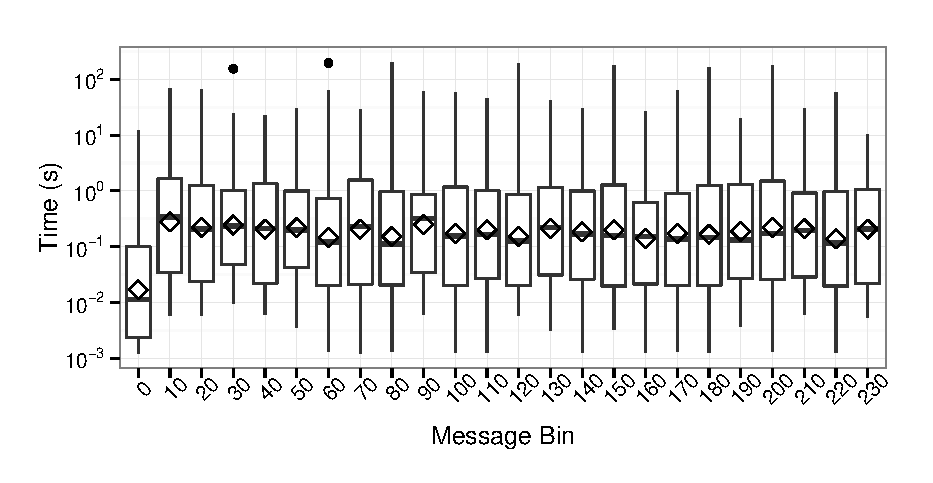
\epsfig{file=figures/ndss13/tetrinet_boxplot_bar_alt_log_Time_Default-Coarse.eps, width=0.6\columnwidth}
} \\[-5pt]
\subfigure[][Hint, $\clusters = \coarseClusterCount$]{
\label{fig:tetrinet:time:hint_coarse}
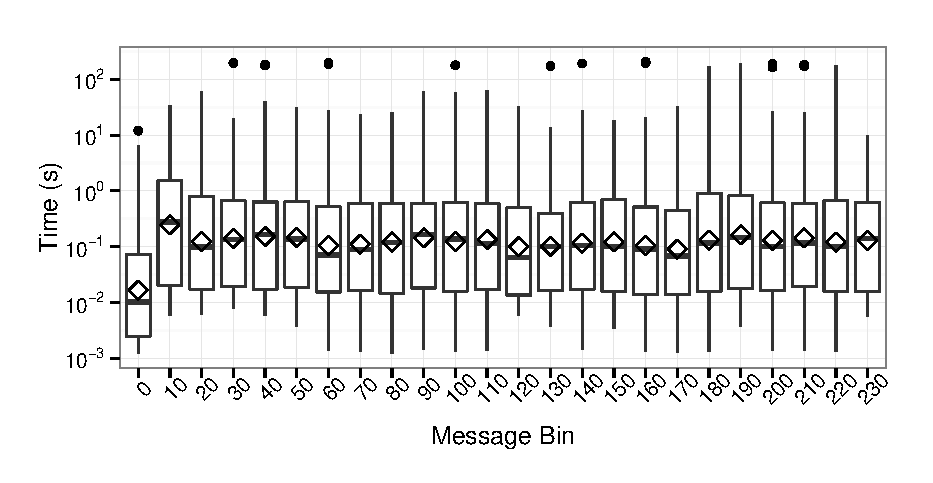
\epsfig{file=figures/ndss13/tetrinet_boxplot_bar_alt_log_Time_Hint-Coarse.eps, width=0.6\columnwidth}
} \\[-5pt]
\subfigure[][Default, $\clusters = \tetrinetFineClusterCount$]{
\label{fig:tetrinet:time:default_fine}
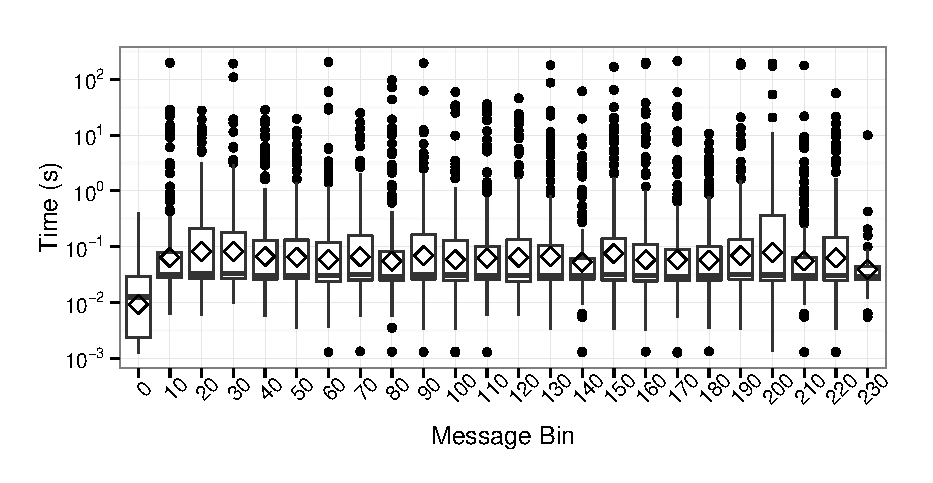
\epsfig{file=figures/ndss13/tetrinet_boxplot_bar_alt_log_Time_Default.eps, width=0.6\columnwidth}
} \\[-5pt]
\subfigure[][Hint, $\clusters = \tetrinetFineClusterCount$]{
\label{fig:tetrinet:time:hint_fine}
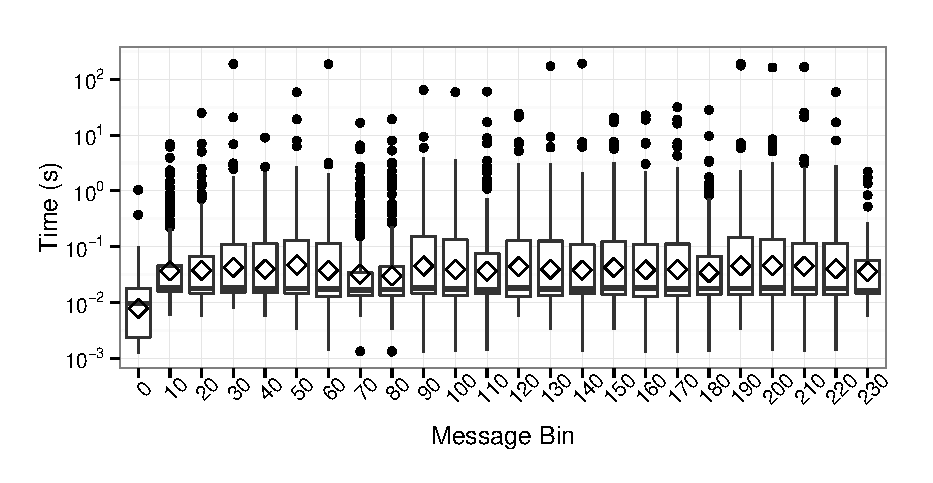
\epsfig{file=figures/ndss13/tetrinet_boxplot_bar_alt_log_Time_Hint.eps, width=0.6\columnwidth}
}\end{tabular}
\caption[\tetrinet verification costs.]{\tetrinet verification costs.
Cross-validation over \tetrinetTraces traces.  Boxplot at \xval shows
verification costs for messages \msg{\xval}, $\ldots$, \msg{\xval+9}
in each trace (after training on the other traces).  ``$\Diamond$''
shows the average.}
\label{fig:tetrinet:time}
\end{figure}


\begin{figure}[t]
\centering
\begin{tabular}{c}
\subfigure[][Default, $\clusters = \coarseClusterCount$]{
\label{fig:tetrinet:delay:default_coarse}
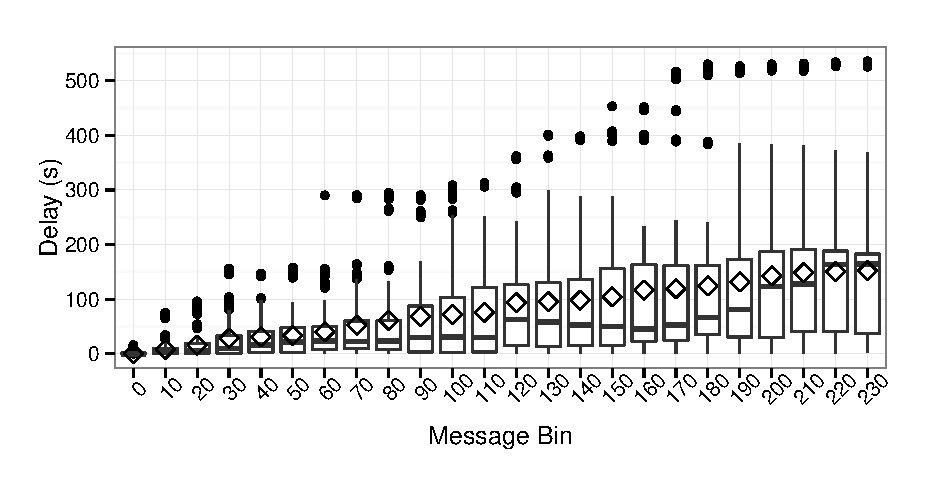
\epsfig{file=figures/ndss13/tetrinet_boxplot_bar_alt_Delay_Default-Coarse.eps, width=0.6\columnwidth}
} \\[-5pt]
\subfigure[][Hint, $\clusters = \coarseClusterCount$]{
\label{fig:tetrinet:delay:hint_coarse}
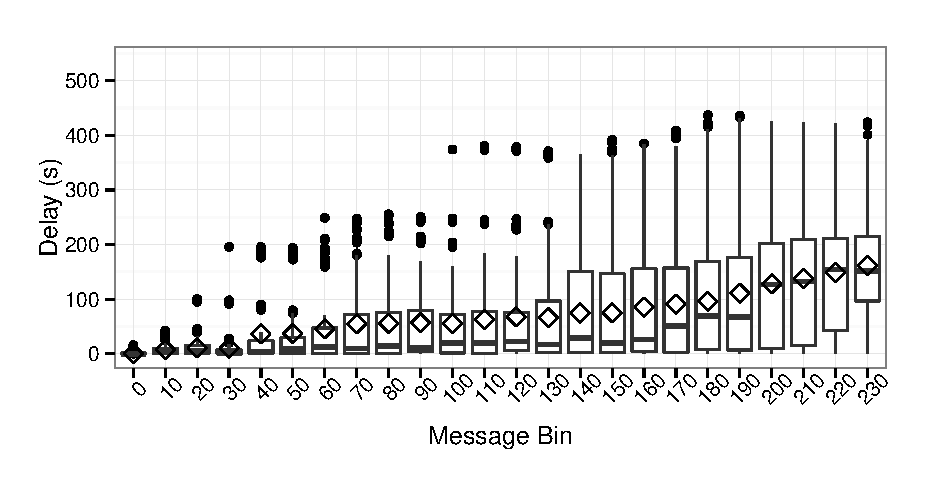
\epsfig{file=figures/ndss13/tetrinet_boxplot_bar_alt_Delay_Hint-Coarse.eps, width=0.6\columnwidth}
} \\[-5pt]
\subfigure[][Default, $\clusters = \tetrinetFineClusterCount$]{
\label{fig:tetrinet:delay:default_fine}
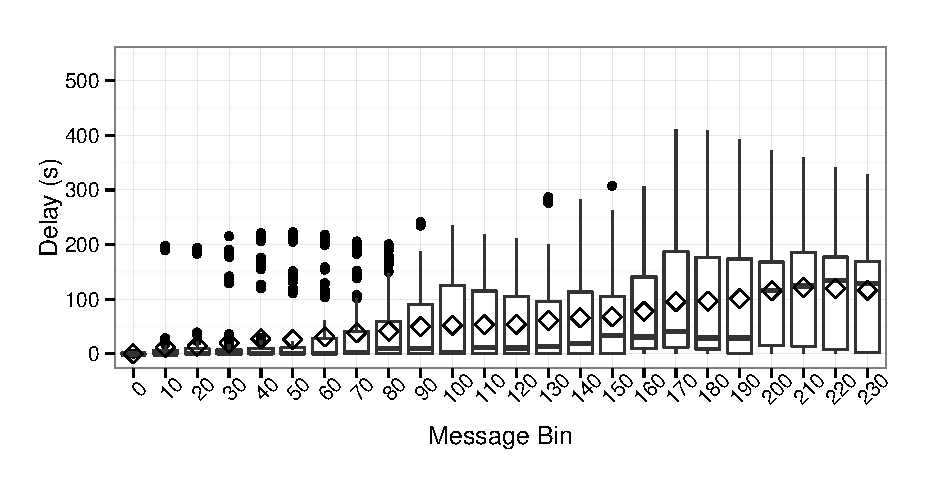
\epsfig{file=figures/ndss13/tetrinet_boxplot_bar_alt_Delay_Default.eps, width=0.6\columnwidth}
} \\[-5pt]
\subfigure[][Hint, $\clusters = \tetrinetFineClusterCount$]{
\label{fig:tetrinet:delay:hint_fine}
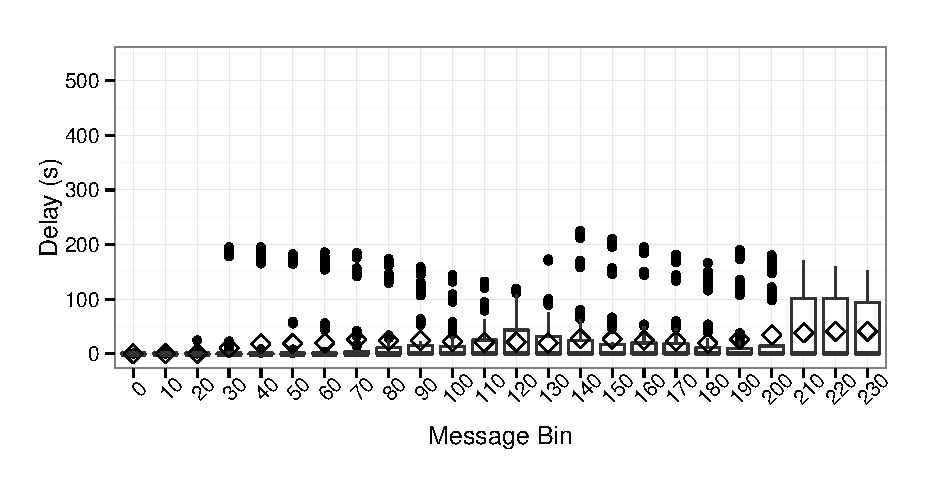
\epsfig{file=figures/ndss13/tetrinet_boxplot_bar_alt_Delay_Hint.eps, width=0.6\columnwidth}
}\end{tabular}
\caption[\tetrinet verification delays]{\tetrinet verification delays.
Cross-validation over \tetrinetTraces traces.  Boxplot at \xval shows
verification delays for messages \msg{\xval}, $\ldots$, \msg{\xval+9}
in each trace (after training on the other traces).  ``$\Diamond$''
shows the average.}
\label{fig:tetrinet:delay}
\end{figure}
\clearpage

To shed light on these issues, \figref{fig:tetrinet:delay} instead
plots the distributions of per-message verification \textit{delay}
between the arrival of message \msg{\msgNmbr} at the server (where a
server-to-client message ``arrives'' when it is sent) and the
discovery of an execution prefix \execPrefix{\msgNmbr} that is
consistent with \msg{0}, $\ldots$, \msg{\msgNmbr}.  Delay
(\figref{fig:tetrinet:delay}) differs from verification cost
(\figref{fig:tetrinet:time}) by representing the fact that
verification for \msg{\msgNmbr} cannot begin until after that for
\msg{\msgNmbr-1} completes.  So, for example, the rightmost boxplot
in each graph provides insight into how long after the completion of
the message trace (in real time) that it took for verification for the
whole trace to complete.

One item to note about these graphs is that for the hint configuration
with $\clusters = \tetrinetFineClusterCount$
(\figref{fig:tetrinet:delay:hint_fine}), the median of the rightmost
boxplot is virtually zero --- i.e., the most common case is that
verification kept pace with gameplay.  This can occur even if
verification falls behind at some point in the game, since
verification commonly ``catches up'' after falling behind. This is
illustrated, for example, in the generally downward slope of
consecutive outlier points in \figref{fig:tetrinet:delay:hint_fine}.
That said, the cumulative effect of verification delays in the other
configurations is more costly, e.g., causing verification to lag
behind gameplay by more than 100 seconds by the end of a
\tetrinetTraceLength-message trace in the median case in the default
configuration (\figref{fig:tetrinet:delay:default_fine}).

A breakdown of verification costs for \tetrinet is shown in
\figref{fig:time_summary}.  In our \tetrinet experiments,
more than 50\% of the verification cost is spent in \klee,
interpreting client instructions.  Therefore, optimizations that
interpret instructions only selectively (e.g.,~\cite{chipounov11:s2e})
may be a significant optimization for our tool.  The majority of the
remaining time is spent in insertions and deletions on \liveSet and in
computing edit distance, both to update the edit distance for each
path when a symbolic branch is reached and to compute distances
between messages.  A very small fraction of time in our \tetrinet
experiments is devoted to equivalent state detection
(\secref{sec:guided:verification:backtracking}) or in constraint solving.  In
\figref{fig:time_summary}, constraint solving includes not only the
time spent by \stp (the default solver used by \klee), but also
preprocessing techniques to make queries to \stp more efficient and a
canonicalization step (similar to Visser et
al.~\cite{visser12:canonicalization}) to improve the hit rate on
cached results for previous queries to \stp.  These optimizations
significantly reduce the overall constraint solving time.

\begin{figure}[H]
\centering
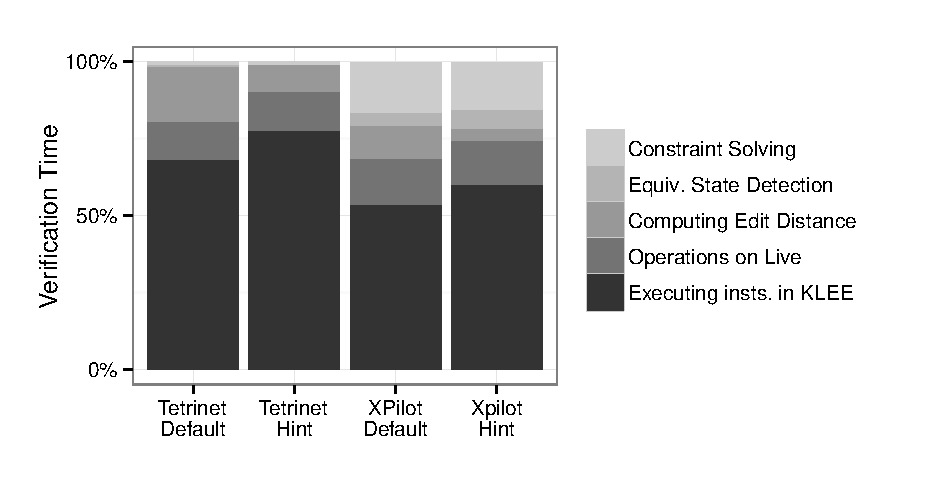
\epsfig{file=figures/ndss13/time_summary.eps, width=0.6\columnwidth}
\caption{Percentage of time spent in each component of the verifier.}
\label{fig:time_summary}
\end{figure}

\subsection{Case Study: \xpilot}
\xpilot poses a significant challenge for verification because its
pace is so fast.  The tests described here use an \xpilot
configuration that resulted in an average of \xpilotMsgsPerSec
messages per second.  The verification costs per message vary somewhat
less for \xpilot than they did for \tetrinet, as shown in
\figref{fig:xpilot:time}.  Recall that each boxplot in
\figref{fig:xpilot:time} represents $100 \times \xpilotTraces$ points,
versus only $10 \times \tetrinetTraces$ in \figref{fig:tetrinet:time}.
As such, though there are larger numbers of outliers in
\figref{fig:xpilot:time}, they constitute a smaller fraction of the
data points.

The median per-message verification cost of \xpilot when clustering is
fine-grained ($\clusters = \xpilotFineClusterCount$, which implied a
single execution fragment per cluster) is quite comparable to that in
\tetrinet, as can be seen by comparing
\figref{fig:xpilot:time:default_fine} and
\figref{fig:xpilot:time:hint_fine} to
\figref{fig:tetrinet:time:default_fine} and
\figref{fig:tetrinet:time:hint_fine}, respectively.  However, \xpilot
verification is considerably faster with coarse clustering, see
\figref{fig:xpilot:time:default_coarse} versus
\figref{fig:tetrinet:time:default_coarse} and
\figref{fig:xpilot:time:hint_coarse} versus
\figref{fig:tetrinet:time:hint_coarse}.  Our definition of $\clusters
= \coarseClusterCount$ as ``coarse'' clustering was dictated by the
goal of limiting the bandwidth overhead to one byte per
client-to-server message in the hint configuration.  The better
performance of \xpilot verification for coarse clustering versus
\tetrinet is at least partly because $\clusters = 256$ is closer to
fine clustering ($\clusters = \xpilotFineClusterCount$) in the case of
\xpilot than it is for \tetrinet ($\clusters = \tetrinetFineClusterCount$).
In the hint configuration, $\clusters = \coarseClusterCount$ increases
bandwidth use by \xpilot client-to-server messages by
\xpilotCoarseBandwidthPerc, and $\clusters = \xpilotFineClusterCount$
(\logXpilotFineClusterCount bits, sent in two bytes) increases it by
\xpilotFineBandwidthPerc.

Though the median per-message verification cost of \xpilot is
generally as good or better than that for \tetrinet, the faster pace
of \xpilot makes it much more difficult for verification to keep pace
with the game.  This effect is shown in \figref{fig:xpilot:delay}.  As
shown in this figure, none of the configurations or clustering
granularities permitted verification to keep up with gameplay, and 
the best default configuration ($\clusters = \xpilotFineClusterCount$)
included one run that required $8$ minutes past the end of the trace to
complete its verification (see
\figref{fig:xpilot:delay:default_fine}).  Consequently, for an
application as fast-paced and as complex as
\xpilot, our algorithm does not eliminate the need to save
traces for post hoc analysis.

Nevertheless, we stress that our algorithm accomplishes --- even if
with some delay --- what is for the approach in \chref{ch:scv}
completely intractable.  That is, recall
that the approach in \chref{ch:scv} utilized a restricted version of \xpilot in which the
number of user inputs per event loop iteration was artificially
limited; we have removed that limitation here (see
\secref{sec:guided:eval:apps}).  With these restrictions removed, the
previous approach is inherently unbounded for verifying some
messages, since it seeks to eagerly find \textit{all} paths that could
explain that message, of which there could be infinitely many.  Our
approach, in contrast, succeeds in verifying all messages in these
logs in bounded time and with per-message cost averaging under
$100\msecs$ in all configurations (\figref{fig:xpilot:time}).

A fractional breakdown of verification costs for \xpilot are shown in
\figref{fig:time_summary}.  While a majority of the cost is still
contributed by interpreting client instructions in \klee, the majority
is smaller in the case of \xpilot than it was for \tetrinet.  For
\xpilot, equivalent state detection
(\secref{sec:guided:verification:backtracking}) plays a more prominent role
than it did for \tetrinet, in part due to \xpilot's more complex memory
structure.  Moreover, due to the substantially more complex
constraints generated by \xpilot, constraint solving plays a much more
prominent role than it did for \tetrinet.

\ignore{
, which is larger in \xpilot which has a more complex memory
structure. Not shown, is the less than 0.5\% of the overall time spent
in the SMT (Satisfiability Modulo Theory) solver; which in our case is
\stp, the default solver used by \klee. The time spent in the SMT
solver is quite low, due largely to the optimizations we preform on
the constraints, which include the canonicalization of variable names
(\secref{sec:guided:canonicalization}), again this optimization takes a
larger portion of the overall verification time in \xpilot.
}

\clearpage
\begin{figure}[t]
\centering
\begin{tabular}{c}
\subfigure[][Default, $\clusters = \coarseClusterCount$]{
\label{fig:xpilot:time:default_coarse}
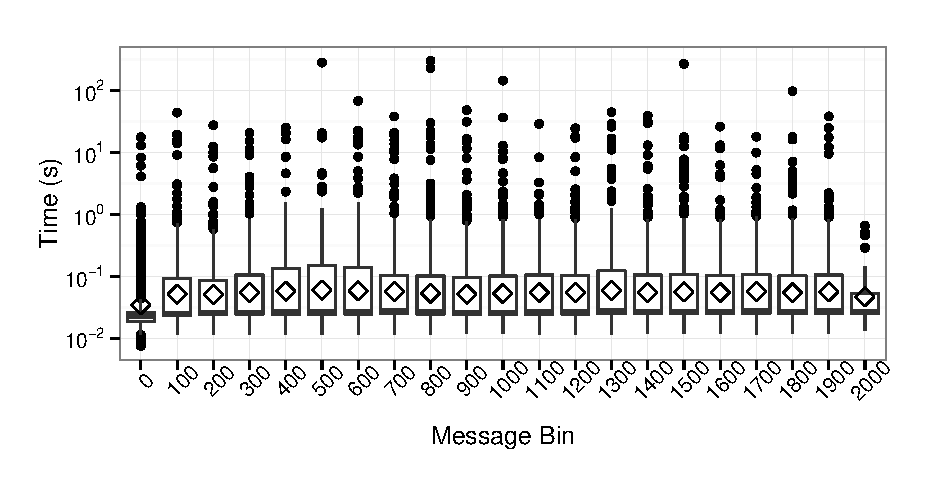
\epsfig{file=figures/ndss13/xpilot_boxplot_bar_alt_log_Time_Default-Coarse.eps, width=0.6\columnwidth}
} \\[-5pt]
\subfigure[][Hint, $\clusters = \coarseClusterCount$]{
\label{fig:xpilot:time:hint_coarse}
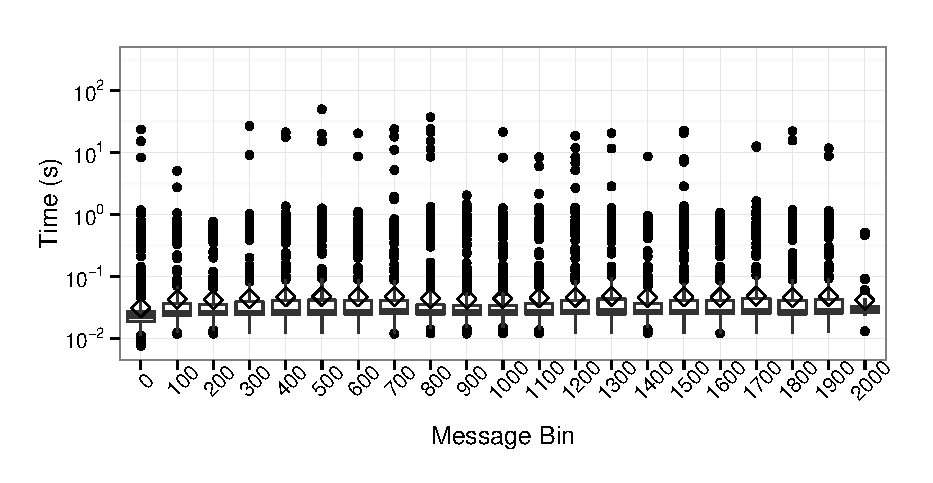
\epsfig{file=figures/ndss13/xpilot_boxplot_bar_alt_log_Time_Hint-Coarse.eps, width=0.6\columnwidth}
} \\[-5pt]
\subfigure[][Default, $\clusters = \xpilotFineClusterCount$]{
\label{fig:xpilot:time:default_fine}
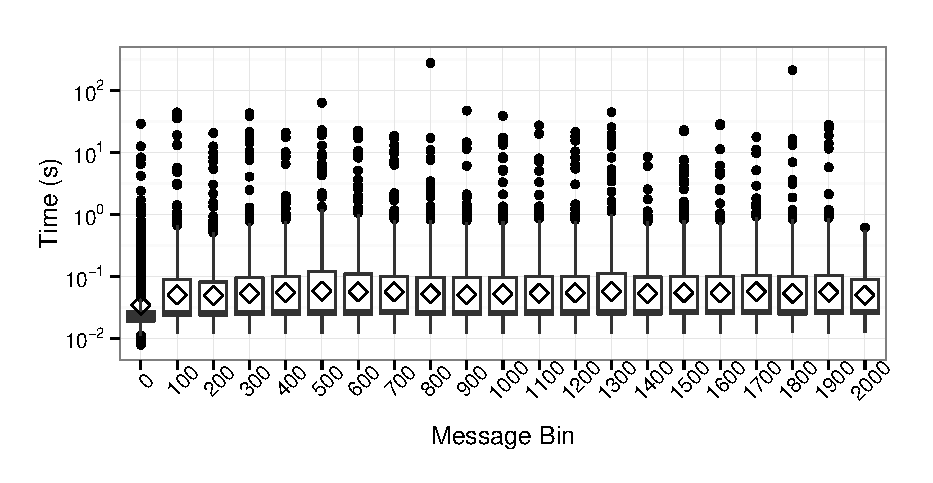
\epsfig{file=figures/ndss13/xpilot_boxplot_bar_alt_log_Time_Default.eps, width=0.6\columnwidth}
} \\[-5pt]
\subfigure[][Hint, $\clusters = \xpilotFineClusterCount$]{
\label{fig:xpilot:time:hint_fine}
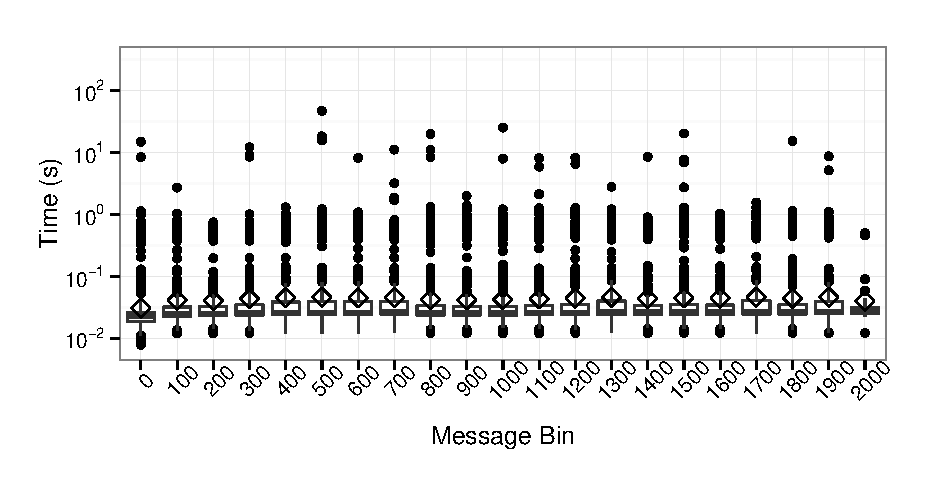
\epsfig{file=figures/ndss13/xpilot_boxplot_bar_alt_log_Time_Hint.eps, width=0.6\columnwidth}
}
\end{tabular}
\caption[\xpilot verification costs]{\xpilot verification costs.
Cross-validation over \xpilotTraces traces.  Boxplot at \xval shows
verification cost for messages \msg{\xval}, $\ldots$, \msg{\xval+99}
in each trace (after training on the other traces).  ``$\Diamond$''
shows the average.}
\label{fig:xpilot:time}
\end{figure}

\begin{figure}[t]
\centering
\begin{tabular}{c}
\subfigure[][Default, $\clusters = \coarseClusterCount$]{
\label{fig:xpilot:delay:default_coarse}
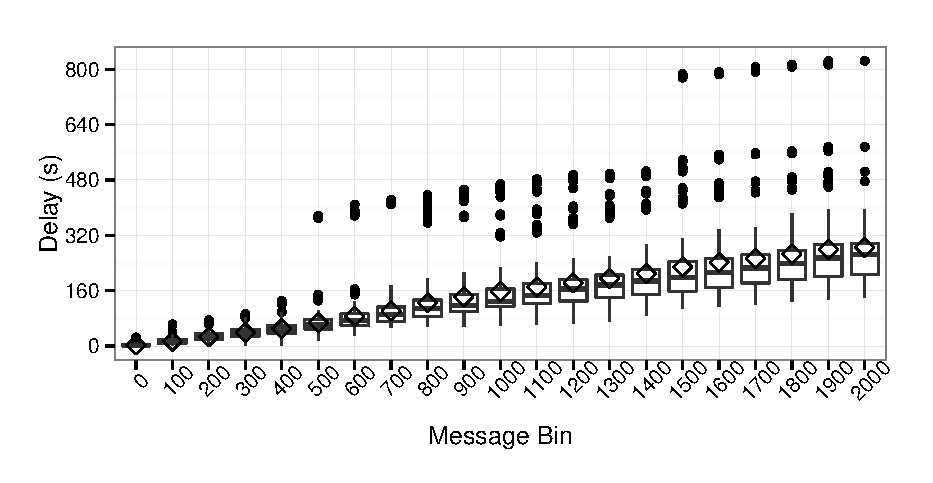
\epsfig{file=figures/ndss13/xpilot_boxplot_bar_alt_Delay_Default-Coarse.eps, width=0.6\columnwidth}
} \\[-5pt]
\subfigure[][Hint, $\clusters = \coarseClusterCount$]{
\label{fig:xpilot:delay:hint_coarse}
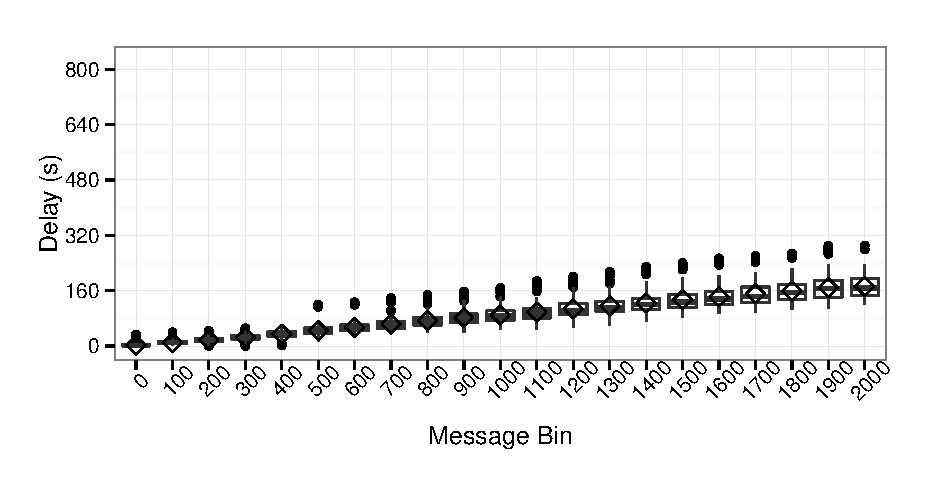
\epsfig{file=figures/ndss13/xpilot_boxplot_bar_alt_Delay_Hint-Coarse.eps, width=0.6\columnwidth}
} \\[-5pt]
\subfigure[][Default, $\clusters = \xpilotFineClusterCount$]{
\label{fig:xpilot:delay:default_fine}
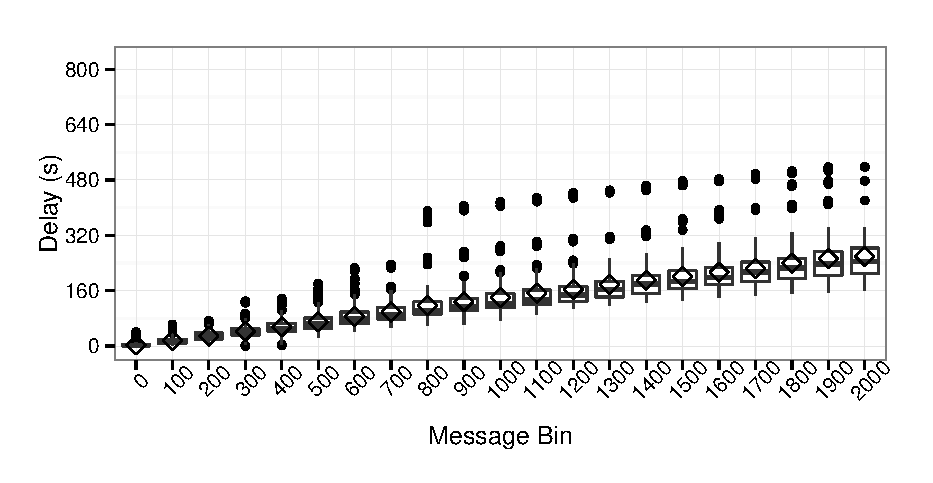
\epsfig{file=figures/ndss13/xpilot_boxplot_bar_alt_Delay_Default.eps, width=0.6\columnwidth}
} \\[-5pt]
\subfigure[][Hint, $\clusters = \xpilotFineClusterCount$]{
\label{fig:xpilot:delay:hint_fine}
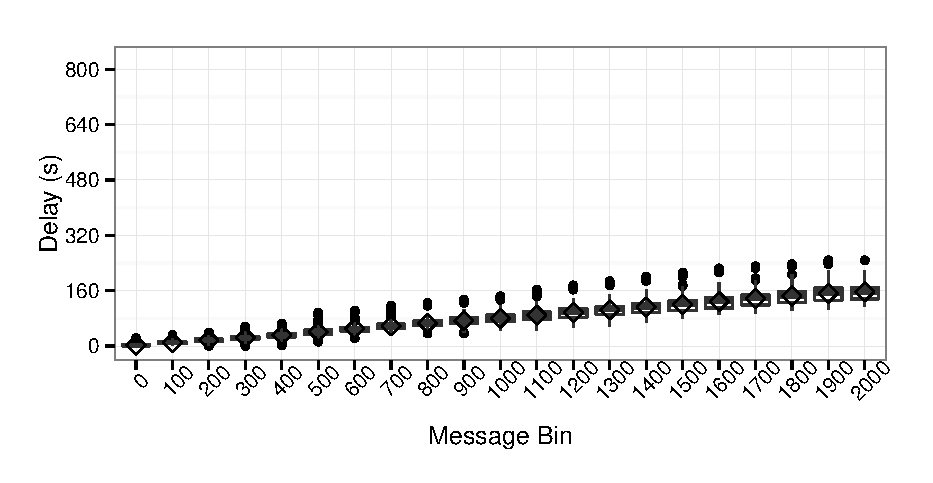
\epsfig{file=figures/ndss13/xpilot_boxplot_bar_alt_Delay_Hint.eps, width=0.6\columnwidth}
}
\end{tabular}
\caption[\xpilot verification delays]{\xpilot verification delays.
Cross-validation over \xpilotTraces traces.  Boxplot at \xval shows
verification delays for messages \msg{\xval}, $\ldots$, \msg{\xval+99}
in each trace (after training on the other traces).  ``$\Diamond$''
shows the average.}
\label{fig:xpilot:delay}
\end{figure}
\clearpage


\section{Summary}
\label{sec:guided:conclusion}

In this \paper we have presented a novel algorithm to enable a server
to verify that the behavior of a client in a client-server application
is consistent with the sanctioned client software.  The central
challenge that must be overcome in achieving this goal is that the
server does not know all of the inputs to the client (e.g., user
inputs) that induced its behavior, and in some domains
(see~\cite{mulligan03:guide}) the additional bandwidth utilized by
sending those inputs to the server is undesirable.  We therefore
developed a technique by which the verifier ``solves'' for whether
there exist user inputs that could explain the client behavior.  We
overcome the scaling challenges of this approach by leveraging execution history
to guide a search for paths through the client program that could
produce the messages received by the server.  This approach enables us to
achieve dramatic cost savings in the common case of a legitimate
client, and by allowing minimal additional bandwidth use, we can
improve performance even further.  In the best configuration of our
algorithm, verification of legitimate \tetrinet gameplay often keeps
pace with the game itself.  In other cases,
verification efficiency is adequate to practically handle client
applications that previous work was forced to restrict to make its
analysis tractable.  We believe that the manner in which we leverage
execution history can be useful in other applications of symbolic
execution, as well.





\chapter{Parallel Client Verification}
\label{ch:par}
Symbolic client verification can be used to build a verifier that
validates traffic received from remote clients. This technique can
identify cheating players in multiplayer networked games or identify other types of
malicious behavior in distributed systems. Client verification is
potentially very useful, especially if the validity result can be
computed quickly. Rather than  logging network traffic for
verification off-line, a fast verifier could be configured  to
validate traffic as it arrives at the server. The contributions of
this \paper are motivated by the goal of keeping a  window of attack
that is as small as possible, or in other words, minimizing the time
it takes the verifier to return a validity result for a given message.
The techniques developed thus far in this dissertation
have not achieved efficiency levels that would allow a
verifier to be placed on the critical path of serving client requests. 

At any point in time during verification, there are many possible
paths of exploration; choosing the right path of exploration improves
the latency of the verifier's result. In the previous \paper we
demonstrated that a combination of training data and edit distance
metrics can be used to guide the verifier's exploration. This approach
is successful because it prioritizes exploration on paths that are
more likely to lead to success. However, this algorithm alone cannot
keep pace with all of our client application case studies. For a
long-running or even continuous client-server session, if the average
time to verify a message is greater than the average time between
message arrivals, the verifier falls further and further behind.
In this \paper, we demonstrate a technique to push forward on multiple
paths of exploration in parallel, resulting in significant performance
improvements. 

The ability to keep pace with client traffic is important because it
opens up new avenues for using our client verification technique. If
the verification is fast enough, it can operate \emph{in-line},
allowing each client-to-server message to be verified as being
consistent with the sanctioned client software, before it is processed
by the server. An in-line verification configuration would add some
amount of latency to the client-to-server network traffic, but that
trade-off may be very acceptable in some situations, especially if the
added latency is low or if the cost of invalid command attacks is very
high. \figref{fig:parallel:inline} shows examples of off-line and
in-line verifier configurations; an in-line configuration
can drop a malicious message before it has time to propagate to
the server. The advantages of in-line client verification include:

\begin{itemize}
  \item Elimination of the need for logging network traffic for later
    verification, reducing storage costs.
  \item Better quality of service for other players in multiplayer games;
    cheaters would be removed more quickly, improving the game
    quality for honest players.
  \item Identification of invalid command messages
    \emph{before} they are processed by potentially vulnerable server
    software, crucially saving server operators from potential damage to
    infrastructure or the leakage of private or sensitive data.
\end{itemize}

\begin{figure}[t]
\centering
\subfigure[][Off-line Client Verification]{
\label{fig:parallel:verifier:offline}
\epsfig{file=figures/parallel/verifier_offline.eps, width=0.7\textwidth}
}
\subfigure[][In-line Client Verification]{
\label{fig:parallel:verifier:inline}
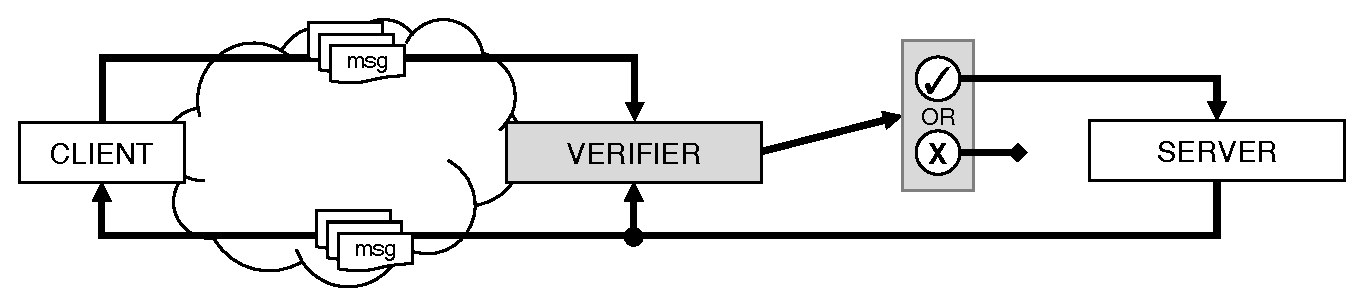
\epsfig{file=figures/parallel/verifier_inline.eps, width=0.7\textwidth}
}
\caption{Off-line and in-line client verification.\label{fig:parallel:inline}}
\end{figure}

\section{Goals and Background}
Our goal is to rapidly identify clients that from the server's
perspective are operating sanctioned client software.
In this \paper we demonstrate that we can achieve
verification results that can keep pace with our case study
applications with a modified version of our verification algorithm. We
describe modifications to our client verification technique to utilize
thread-level parallelism. Although using training data can reduce the
total number of execution states that must be explored, we also wish
to further reduce the time between message arrival and the
verification result. Concurrent exploration can achieve this result.

The outline of the rest of this \paper is as follows.
We will first review the client verification problem and
describe the architecture of our verifier. We then review
multi-threading primitives and describe an algorithm for parallel
client verification in detail. Following that are an overview
of implementation level details and then an evaluation on two
client case studies, \tetrinet and \xpilot.


\subsection{Client Verification Overview}
\label{sec:par:overview}

We now state our assumptions, describe the architecture of the verifier
and the client verification problem.

\subsubsection{Assumptions}
As in the previous chapter,
we are concerned with verifying a client that generates a message
trace, \msg{0}, \msg{1}, $\ldots$, \msg{\msgNmbr}, some sent by the
client and some sent by the server. Furthermore, as before, we assume
the software running on the remote client is single-threaded and that
the verifier is provided with an ordering of messages according to the
client's perspective.

\begin{figure}[t]
\centering
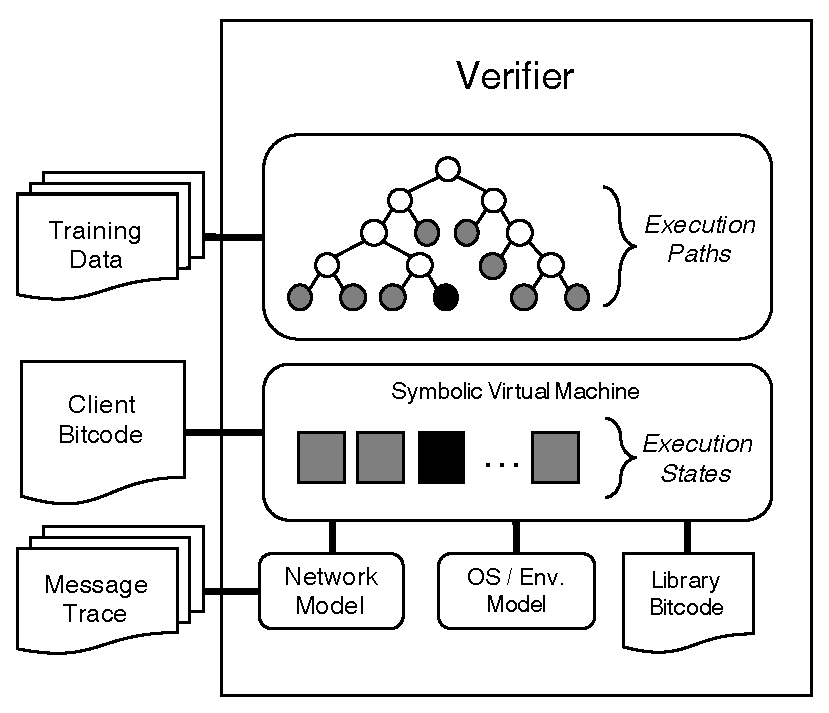
\epsfig{file=figures/parallel/verifier_architecture.eps, width=0.4\columnwidth}
\caption{Verifier Architecture\label{fig:parallel:verifier:arch}}
\end{figure}

\subsubsection{Architecture and Assumptions}
In previous \papers, we have described the verifier architecture shown
in \figref{fig:parallel:verifier:arch}. The verifier operates by
exploring possible execution paths the client may have taken to find a
path that ``explains'' a given message trace. If no such path can be
found, the message trace is declared invalid. The verifier uses
symbolic execution to explore possible client paths. To operate, the
verifier requires three inputs; a message trace, \msgTrace, which will
be verified; the source code for some sanctioned client software,
compiled into an intermediate representation (IR) that can be executed
by a symbolic virtual machine; and a set of training data for
the client bitcode under verification that is used to guide the
selection of possible paths of execution. The message trace is
incrementally fed to the verifier as it arrives at the server and
the verifier outputs if the message trace it has processed thus far can be
explained by an execution path in the software that the client is
expected to be running. 

\subsubsection{Client Verification Definition}
\label{sec:par:definitions}

We formally define the task of the verifier using the same definitions
as \chref{ch:guided}. The verifier's algorithm determines whether
there exists an \textit{execution prefix} of the client that is
\textit{consistent} with the messages $\msg{0}, \msg{1}, \ldots$,
\msg{\msgNmbr}.  Specifically, an execution prefix
\execPrefix{\msgNmbr} is a sequence of client instructions that begins
at the client entry point and follows valid branching behavior in the
client program. We define \execPrefix{\msgNmbr} to be
\textit{consistent} with \msg{0}, \msg{1}, $\ldots$, \msg{\msgNmbr},
if the network \sendInstr and \recvInstr instructions\footnote{We
abbreviate call instructions to POSIX \posixSelect, \posixSend and
\posixRecv system calls (or their functional equivalents) with the
labels \selInstr, \sendInstr and \recvInstr.} in \execPrefix{\msgNmbr}
number $\msgNmbr+1$ and  these network instructions match \msg{0},
\msg{1}, $\ldots$, \msg{\msgNmbr} by direction---i.e., if
\msg{\msgIdx} is a client-to-server message (respectively,
server-to-client message), then the \msgIdx-th network I/O instruction
is a \sendInstr (respectively, \recvInstr)---and if the branches taken
in \execPrefix{\msgNmbr} were possible. Consistency of
\execPrefix{\msgNmbr} with \msg{0}, \msg{1}, $\ldots$, \msg{\msgNmbr}
requires that the conjunction of all symbolic postconditions at
\sendInstr instructions along \execPrefix{\msgNmbr} be satisfiable,
once concretized using the contents of messages \msg{0}, \msg{1},
$\ldots$, \msg{\msgIdx} sent and received on that path. 

The verifier attempts to validate the sequence \msg{0}, \msg{1},
$\ldots$ incrementally, by verifying the sequence \msg{0},
\msg{1}, $\ldots$, \msg{\msgNmbr} starting from an execution prefix
\execPrefix{\msgNmbr-1} found to be consistent with \msg{0}, \msg{1},
$\ldots$, \msg{\msgNmbr-1}, and appending to it an \textit{execution
fragment} that yields an execution prefix \execPrefix{\msgNmbr}
consistent with \msg{0}, \msg{1}, $\ldots$, \msg{\msgNmbr}.
Specifically, an \textit{execution fragment} is a nonempty sequence of
client instructions (i) beginning at the client entry point, a
\selInstr, or a \sendInstr in the client software, (ii) ending at a
\sendInstr or \recvInstr, and (iii) having no intervening \sendInstr
or \recvInstr instructions.  This incremental mechanic is important to
note, as it is the key step in the verification algorithm that we
describe. By using an incremental construction, an entire execution
prefix \execPrefix{\msgNmbr} can be constructed if a given message
trace was produced by a valid client. The verification algorithm
operates as a step-by-step construction of an execution prefix,
because when verification begins, the verifier will only have a single
network message \msg{0}.

\subsubsection{Client Verification Backtracking}
Suppose an execution prefix \execPrefix{\msgNmbr-1} is consistent with
a message trace up to message \msg{\msgNmbr-1}. It is possible for
there to be no execution fragment that can be appended to produce an
execution prefix \execPrefix{\msgNmbr} that is consistent with the
message trace extended by the next message to arrive, \msg{\msgNmbr}.
Intuitively, a path of execution may exercise
client state that precludes future client actions or outputs from
occurring. The verifier incrementally constructs an execution prefix
in an optimistic fashion. In many cases, there is more than one
execution prefix consistent with a message trace, but the verifier
only needs to find one to show that a client is valid. When the
verifier cannot find an execution fragment that can be appended to
\execPrefix{\msgNmbr-1} to produce a \execPrefix{\msgNmbr} consistent
with \msg{0}, \msg{1}, $\ldots$, \msg{\msgNmbr}, then the verifier
backtracks to find a new \execPrefixAlt{\msgNmbr-1} consistent with
\msg{0}, \msg{1}, $\ldots$, \msg{\msgNmbr-1} that can be extended with
an execution fragment to yield a \execPrefixAlt{\msgNmbr} consistent
with \msg{0}, \msg{1}, $\ldots$, \msg{\msgNmbr}.  Only after all such
attempts fail can the client behavior be declared invalid, which may
take substantial time. In practice, an ``invalid'' declaration usually
comes by timeout on the verification process. Our concern in this
\paper is verifying the behavior of \textit{valid} clients quickly,
irrespective of how long it requires to declare an invalid client as
such.

\section{Parallel Client Verification }

We now present a verification algorithm that takes advantage of
thread-level parallelism. At a high level, the main work of
verification is symbolically executing client code to produce an
execution prefix (\secref{sec:par:definitions}) for a given
message sequence. The algorithm that we describe outlines the steps
required to produce an execution prefix \execPrefix{\msgNmbr} from an
execution prefix \execPrefix{\msgNmbr-1}. In practice, many possible
paths of execution need to be explored to produce an execution
fragment. Incomplete paths will be dropped upon reaching unsatisfiable
states and candidate execution fragments will be dropped if the
network action at the end of the fragment is not consistent with the
message trace. Our parallel client verification algorithm
achieves significant improvements in performance by using
thread-level parallelism to explore candidate execution fragments.

\begin{figure}[t]
\centering
\subfigure[][Node data structure]{
\begin{minipage}{0.4\textwidth}
\vspace{15pt}
\begin{tabbing}
\hspace{1em}\=\hspace{9em}\=\kill
\Struct \NodeType $\{$ \\
\> \SymbolicStateType     \> $\sf{state}$; \\
\> \ExecutionFragmentType \> $\sf{path}$; \\
\> \Struct \NodeType      \> $\sf{child[2]}$; \\
$\}$
\end{tabbing}
\vspace{15pt}
\end{minipage}
}
\subfigure[][Node tree with multiple workers attached]{
\centering
\begin{minipage}{0.6\textwidth}
\centering
\epsfig{file=figures/parallel/parallel_node_tree.eps, width=0.84\textwidth}
\vspace{10pt}\end{minipage}
}\
\caption{Node data structure and node tree.
\label{fig:parallel:node}}
\end{figure}

\subsection{Algorithm Definitions}

We now define the data structures used by the algorithm. A 
state \symState{} represents a snapshot of execution in the symbolic
virtual machine, including all constraints (path conditions) and memory
objects, which includes the contents (symbolic or concrete) of
registers, the stack and the heap. The verifier produces state
\symState{\msgNmbr} by symbolically executing the instruction sequence
represented by execution prefix \execPrefix{\msgNmbr}.

The algorithm builds and maintains binary tree,
consisting of \Node objects, shown in \figref{fig:parallel:node}{(a)}.
This tree
is rooted with a state \symState{\msgNmbr-1} and an empty path.
\figref{fig:parallel:node}{(b)} shows an example tree, with a root
node containing \symState{\msgNmbr-1}. (The remaining
node types will be described later in the algorithm description.)
The two children of a node in the tree extend \execPrefix{\msgNmbr-1},
the path represented by \symState{\msgNmbr-1}, 
 through the next symbolic branch (i.e., branch instruction with
 a symbolic condition). One child state holds a constraint
that maintains that the branch condition implies false, and the other
child state holds a constraint that indicates that the branch
condition is true. The algorithm succeeds by finding a fragment with
which to extend \execPrefix{\msgNmbr-1} to yield \execPrefix{\msgNmbr}
if, upon extending a path, it encounters a network I/O instruction
that yields a state with constraints that do not contradict
\msg{\msgNmbr} being the network I/O instruction's message.

We define a set of training data \trainingFrags{} to be a set of
execution fragments and associated message data, observed and
collected via execution of the client prior to verification.
During verification, the verifier selects a subset of execution
fragments $\trainingFrags{\msgNmbr} \subseteq \trainingFrags{}$, for
verification of \msg{\msgNmbr}. The set \trainingFrags{\msgNmbr} is
used prioritize nodes in the node tree rooted at
\symState{\msgNmbr-1}. This prioritization technique is detailed in
\chref{ch:guided}.

\subsection{Key Insights}
The driving goal of our algorithm is to enable concurrent exploration
of multiple states in the node tree. The sooner the algorithm can
explore and then eliminate candidate paths, the sooner it can find a
valid execution fragment. We designed the parallel verification
algorithm to use multiple threads; it uses a single thread to manage
the node tree, a single thread to select the training data subset, and
several worker threads, each assigned to a single node in the node
tree at time. \figref{fig:parallel:node}{(b)} shows an example
assignment of four workers to multiple nodes in a node tree. In our
design and experiments the number of worker threads \workerCount is a
fixed parameter provided to the verifier. Because the verification
task is largely CPU-bound, it is in our experience not beneficial to
use more worker threads than the number of logical CPU cores, and in
some cases, fewer worker threads than cores are necessary. The main
objective of our design is to get ``out of the way'' of the worker
threads. What follows are the high level features of the design.

\begin{itemize}

\item {\bf Concurrent exploration of execution fragments:}
The most important contribution of the algorithm is concurrent
exploration of execution fragments rooted at \symState{\msgNmbr-1}. This
is enabled by a multi-threaded symbolic execution engine (detailed in
\secref{sec:par:klee}). As designed, the algorithm explores only
execution fragments starting from one state \symState{\msgNmbr-1}
corresponding to one execution prefix \execPrefix{\msgNmbr-1}.
Although searching from multiple execution prefixes is not
fundamentally impossible, our implementation of backtracking requires
all worker threads to be exploring fragments in the same node tree.

\item {\bf Non-blocking node tree management:} 
Operations on the node tree operate asynchronously from the worker
threads. This is done so that worker threads do not have to block on
operations that interact with shared data structures. 

\item {\bf Non-blocking training data selection:} 
The parallel verification algorithm extends the method of training
data selection described in \chref{ch:guided}. As before, when
\msg{\msgNmbr} arrives, the verifier selects from a set of execution
fragments \trainingFrags{}, produced during training, that are deemed
likely to be similar to the fragment executed by the client leading up
to it sending or receiving \msg{\msgNmbr}; this subset of execution
fragments is denoted \trainingFrags{\msgNmbr}. Depending on the
size of the training data and granularity of clustering, the selection
of \trainingFrags{\msgNmbr} may take a significant amount of time. The
parallel verification algorithm asynchronously selects
\trainingFrags{\msgNmbr} in a separate thread so that the exploration
from \symState{\msgNmbr-1} is not blocked and can begin before
\trainingFrags{\msgNmbr} is available. Once \trainingFrags{\msgNmbr}
has been computed, the node selection algorithm switches from naive
breadth-first search to an edit-distance search using the selected
subset of execution fragments (\trainingFrags{\msgNmbr}).

 
\end{itemize}

\subsection{Multi-threading primitives}
\label{sec:par:multithreaddefinitions}

The description of our algorithm requires the definition of primitives
used in the dynamic multi-threading model~\cite{cormen09:alg}. These
primitives are $\Spawn$, $\Sync$ and $\Atomic$. The keyword $\Spawn$
must precede a procedure call and has semantics such that the next
statement may continue execution concurrently with the spawned
procedure. In other words, $\Spawn$ indicates the creation of a child
thread that will execute the declared procedure until completion, at
which point the child thread will terminate. The second keyword
$\Sync$ denotes that the parent procedure will wait to proceed to the
next statement until all spawned child threads have finished
execution.  The keyword \Atomic is necessary because, when executing in a
multi-threaded environment, multiple threads may access the same
memory locations at once. In order for concurrent threads to safely
change such a value, a thread that loads and modifies a variable
should execute these operations atomically, in isolation from the rest
the threads. We use the keyword $\Atomic$ in our algorithm description
to indicate that an operation or sequence of operations must execute with
the appearance to other threads of occurring instantaneously. Note
that this is a simplification of the underlying implementation, which
may make use of compare-and-swap operations, mutexes and condition
variables to achieve thread-safe memory operations.


%\algrenewcommand\algorithmicindent{0.5em}%
\begin{figure}[ht]
\begin{minipage}{\textwidth}
\begin{algorithm}[H] % must use H inside minipage
  \caption{Parallel Client Verification}
  %\label{algmultipass}
\begin{algorithmic}[1]
\setalglineno{300}
\Procedure{\parallelVerifyAlg}{\symState{\msgNmbr-1}, 
                               \msg{\msgNmbr}, \trainingFrags{}}
  \label{fig:paralg:parallelVerifyAlg}
  \State $\activeCount \gets 0$
    \Comment{Number of active threads}
    \label{fig:paralg:initWait}
  \State \Atomic $\readyQ \gets \makeNodeQueue()$
    \Comment{Nodes for worker threads to execute}
    \label{fig:paralg:initReady}
  \State \Atomic $\addedQ \gets \makeNodeQueue()$
    \Comment{Nodes created by worker threads}
    \label{fig:paralg:initAdded}
  \State \Atomic $\validState \gets \bot$
    \Comment{Will be set to a valid path if successful}
    \label{fig:paralg:initValid}
  \State \Atomic $\verifyFinished \gets \codeFalse$
    \Comment{Instructs all threads to halt}
    \label{fig:paralg:initFinished}
  \State $\trainingFrags{\msgNmbr} \gets \{\}$
    \Comment{Training for  set \msg{\msgNmbr}}
    \label{fig:paralg:initTraining}
  \State \Spawn \Call{\clusterSelector}{\msg{\msgNmbr}, 
                                        \trainingFrags{}, 
                                        \trainingFrags{\msgNmbr}} 
    %\Comment{Select clusters based on \msg{\msgNmbr}} 
    \label{fig:paralg:spawnClusterSelector}
  \State \Spawn \Call{\nodeScheduler}{\symState{\msgNmbr-1}, 
                                      \trainingFrags{\msgNmbr}, 
                                      \readyQ, \addedQ, 
                                      \activeCount, \verifyFinished}
    %\Comment{Initialize Node Scheduler} 
    \label{fig:paralg:spawnNodeScheduler}
  \For{1 \textbf{to} \workerCount}
    %\Comment{Spawn worker threads} 
    \State \Spawn \Call{\verifyWorker}{\msg{\msgNmbr}, 
                                       \readyQ, \addedQ, 
                                       \activeCount, \verifyFinished, 
                                       \validState}
      \label{fig:paralg:spawnVerifyWorker}
  \EndFor
  \State \Sync
    \Comment{Wait for all child threads} 
    \label{fig:paralg:sync}
  \State \Return \validState
    \Comment{Return result, $\bot$ or \symState{\msgNmbr}}
    \label{fig:paralg:returnValid}
\EndProcedure
\Statex
\end{algorithmic}
\end{algorithm}
\end{minipage}
\caption{Main procedure for parallel client verification.
\label{fig:paralg}}
\end{figure}


\subsection{Details of parallel verification algorithm} 
\label{sec:par:verifydetails}

The algorithm for verifying a client-to-server message using
thread-level parallelism is shown in \figref{fig:paralg}. This
algorithm, denoted \parallelVerifyAlg, takes as input the symbolic
state \symState{\msgNmbr-1} resulting from execution of
\execPrefix{\msgNmbr-1} from the client entry point on message trace
$\msg{0},\ldots,\msg{\msgNmbr-1}$, the next message \msg{\msgNmbr};
and the complete training fragment set \trainingFrags{}.  Its output
is either an execution fragment that can be appended to
\execPrefix{\msgNmbr-1} to make \execPrefix{\msgNmbr} that is
consistent with \msg{0}, $\ldots$, \msg{\msgNmbr}, or no solution 
($\bot$).  The latter case indicates failure and, more specifically,
that there is no execution prefix that can extend
\execPrefix{\msgNmbr-1} to make \execPrefix{\msgNmbr} that is
consistent with \msg{0}, $\ldots$, \msg{\msgNmbr-1}.  This will induce
backtracking to search for another \execPrefixAlt{\msgNmbr-1} that
is consistent with \msg{0}, $\ldots$, \msg{\msgNmbr-1}, which the
verifier will then try to extend to find a \execPrefix{\msgNmbr}
consistent with \msg{0}, $\ldots$, \msg{\msgNmbr}. 

The algorithm operates in a parent thread that spawns $\workerCount+2$
child threads; this includes one thread to select training data, one
thread to manage scheduling of nodes for execution, and \workerCount
worker threads to explore candidate execution fragments.
We outline in detail the operation of algorithm
\parallelVerifyAlg below.

\begin{description}
\item[Initialization:]
First, variables that will be passed to the algorithm sub-procedures
are initialized (Lines
\ref{fig:paralg:initWait}--\ref{fig:paralg:initFinished}). This
includes a counter \activeCount that tracks the number of active
workers (\ref{fig:paralg:initWait}), two empty \NodeType queues
\readyQ  and \addedQ
(\ref{fig:paralg:initWait}--\ref{fig:paralg:initAdded}), an object
\validState that will be set to a valid execution fragment if the algorithm is
successful (\ref{fig:paralg:initValid}) and a boolean \verifyFinished
that will be set to \codeTrue when the algorithm reaches a stop condition
(\ref{fig:paralg:initFinished}). 
%All of these variables may be updated concurrently and thus such operations must use \Atomic.

\item[Training Set Selection Thread:]
Next, on line \ref{fig:paralg:spawnClusterSelector}, a thread is
spawned for \clusterSelector. This procedure selects a set of training
fragments $\trainingFrags{\msgNmbr} \subseteq \trainingFrags{}$ from
the set of all training fragments \trainingFrags{} based on the
contents of the message \msg{\msgNmbr}. The details of this algorithm
are outlined in \chref{ch:guided}. The important change here is that
this algorithm is run in separate thread. We will outline the
intuition behind this choice below. 

\item[Node Selection Thread:] 
The algorithm then spawns a procedure that manages the selection of
nodes to execute next (\ref{fig:paralg:spawnNodeScheduler}). The
parameters to \nodeScheduler are training fragment set
\trainingFrags{\msgNmbr}, node queues \readyQ and \addedQ, counter
\activeCount and boolean \verifyFinished. Procedure \nodeScheduler is
spawned in a child thread so that operations on the node tree do not
block state exploration.

\item[Verification Worker Threads:]
Finally, the algorithm spawns a fixed number of threads that execute
the \verifyWorker procedure (\ref{fig:paralg:spawnVerifyWorker}). This
procedure takes as parameters: network message \msg{\msgNmbr}, node
queues \readyQ and \addedQ, counter \activeCount, boolean
\verifyFinished and execution path \validState. 

\item[Termination:]
Execution is blocked at the call \Sync until all child threads have
exited due to a termination condition, namely $\verifyFinished =
\codeTrue$. After all child threads
have finished the algorithm returns the result \validState, which is
either set by a worker thread to an execution fragment \newPath, that
when appended to \execPrefix{\msgNmbr-1}
is consistent with \msg{0}, $\ldots$, \msg{\msgNmbr} or on
failure, remains undefined $\bot$ as initialized.

\end{description}
\clearpage
%%%%%%%%%%%%%%%%%%%%%%%%%%%%%%%%%%%%%%%%%%%%%%%%%%%%%%%%%%%%%%%%%%%%%%%%
\begin{figure}[ht]
\begin{minipage}{\textwidth}
\begin{algorithm}[H] % must use H inside minipage
\caption{Parallel Client Verification (sub-procedures)}
\begin{algorithmic}[1]
\setalglineno{400}

\Procedure{\nodeScheduler}{\symState{\msgNmbr-1}, \trainingFrags{}, \readyQ, \addedQ, \activeCount, \verifyFinished}
  \label{fig:paralg:nodeScheduler}
  \State $\node \gets \makeNode()$
  \label{fig:paralg:makeRoot}
  \State $\node.\pathField \gets \langle\rangle$; $\node.\stateField \gets \symState{\msgNmbr-1}$
  \label{fig:paralg:initRoot}
  \State $\liveSet \gets \{\node\}$
  \label{fig:paralg:initLiveSet}
  \While{$\verifyFinished =  \codeFalse$}
  \label{fig:paralg:nodeSchedulerWhile}
    \If{$|\liveSet| > 0$ \codeAnd $|\readyQ| < (\workerCount - \activeCount)$}
    \label{fig:paralg:ifEnqueueReady}
      %\State $\displaystyle \node \gets \arg \min_{\nodeAlt \in \liveSet} \min_{\trainingFrag \in \trainingFrags{\msgNmbr}} \min_{\trainingFragAlt \prefixOf \trainingFrag} \editDist(\nodeAlt.\pathField, \trainingFragAlt)$ \\
    \State $\node \gets$ \Call{\selectNode}{\liveSet, \trainingFrags{\msgNmbr}}
    \label{fig:paralg:editDist}
      \State \Atomic $\enqueue(\readyQ, \node)$ 
      \label{fig:paralg:enqueueReady}
    \EndIf
    \While{$|\addedQ| > 0$}
    \label{fig:paralg:ifAdded}
      \State \Atomic $\liveSet \gets \liveSet \cup \{\dequeue(\addedQ)\}$
      \label{fig:paralg:dequeueAdded}
    \EndWhile
    \If{$|\liveSet| = 0$ \codeAnd $|\readyQ| = 0$ \codeAnd $|\addedQ| = 0$ \codeAnd $\activeCount = 0$}
    \label{fig:paralg:ifEmpty}
      \State $\verifyFinished \gets \codeTrue$
      \label{fig:paralg:emptyLive}
    \EndIf
  \EndWhile
\EndProcedure

\State

\Procedure{\verifyWorker}{\msg{\msgNmbr}, \readyQ, \addedQ, \activeCount, \verifyFinished, \validState}
\label{fig:paralg:verifyWorker}
\While{$\verifyFinished = \codeFalse$}
  \label{fig:paralg:verifyWorkerWhile}
  \If{$|\readyQ| > 0$}
  \label{fig:paralg:ifDequeueReady}
    \State \Atomic $\activeCount \gets \activeCount + 1$
    \State \Atomic $\node \gets \tryDequeue(\readyQ)$
    \label{fig:paralg:dequeue}
    \If{$\node \neq \bot$}
      \label{fig:paralg:ifNode}
      \State $\newPath \gets \node.\pathField$ ; $\newState \gets \node.\stateField$ 
      \While{$\isIOInstruction(\newState.\nextInstruction) = \codeFalse$ \codeAnd $\isSymbolicBranch(\newState.\nextInstruction) = \codeFalse$}
        \label{fig:paralg:whileSymEx}
        \State $\newPath \gets \newPath \parallel \langle \newState.\nextInstruction \rangle$
        \label{fig:paralg:extendPath}
        \State $\newState \gets \execStep(\newState)$
        \label{fig:paralg:execStep}
      \EndWhile
      
      \If{$\isIOInstruction(\newState.\nextInstruction) = \codeTrue$}
      \label{fig:paralg:isIOInstruction}
        \If{$((\newState.\constraints\wedge\newState.\nextInstruction.\messageVar= \msg{\msgNmbr}) \not\Rightarrow \codeFalse)$}
          \State $\verifyFinished \gets \codeTrue$
          \State $\validState \gets \newState$
          \label{fig:paralg:returnSuccess}
          \Comment{Success!}
          %\State $\validPath \gets \newPath \parallel \langle \newState.\nextInstruction \rangle$
          %\State \Return 
        \EndIf
      \ElsIf{$\isSymbolicBranch(\newState.\nextInstruction) = \codeTrue$}
        \label{fig:paralg:isSymbolicBranch}
        %\State $\node.\childField{0} \gets \makeNode(\newState, \newState.\nextInstruction.\condition \mapsto \codeFalse)$
        %\State $\node.\childField{0} \gets \makeNode()$
        %\label{fig:paralg:makeChildFalse}
        \State $\node.\childField{0}.\stateField \gets [~\execStep(\newState)~\mid$ $\newState.\nextInstruction.\condition \mapsto \codeFalse~]$
        \label{fig:paralg:branchFalse}
        %\State $\node.\childField{0}.\pathField \gets \newPath \parallel \langle \newState.\nextInstruction \rangle$
        \State $\node.\childField{0}.\pathField \gets \newPath \parallel \langle \node.\childField{0}.\stateField.\nextInstruction \rangle$
        \label{fig:paralg:pathExtendFalse}
        \If{$\node.\childField{0}.\stateField.\constraints \not\Rightarrow \codeFalse$}
        \label{fig:paralg:checkFalse}
          \State \Atomic $\enqueue(\addedQ, \node.\childField{0})$
          \label{fig:paralg:addFalse}
        \EndIf
        %\State $\node.\childField{1} \gets \makeNode(\newState, \newState.\nextInstruction.\condition \mapsto \codeTrue)$
        %\State $\node.\childField{1} \gets \makeNode()$
        %\label{fig:paralg:makeChildTrue}
        \State $\node.\childField{1}.\stateField \gets [~\execStep(\newState)~\mid$ $\newState.\nextInstruction.\condition \mapsto \codeTrue~]$
        \label{fig:paralg:branchTrue}
        \State $\node.\childField{1}.\pathField \gets \newPath \parallel \langle \node.\childField{1}.\stateField.\nextInstruction \rangle$
        \label{fig:paralg:pathExtendTrue}
        \If{$\node.\childField{1}.\stateField.\constraints \not\Rightarrow \codeFalse$}
        \label{fig:paralg:checkTrue}
          \State \Atomic $\enqueue(\addedQ, \node.\childField{1})$
          \label{fig:paralg:addTrue}
        \EndIf

      \EndIf
    \EndIf
    \State \Atomic $\activeCount \gets \activeCount - 1$
  \EndIf

\EndWhile
\label{fig:paralg:mainWhileEnd}
\EndProcedure

\end{algorithmic}
\end{algorithm}
\end{minipage}
\caption{Sub-procedures for parallel client verification.\label{fig:paralg:sub}}
\end{figure}
\clearpage


\subsection{Details of parallel verification algorithm sub-procedures} 
\label{sec:par:nodedetails}

We now describe in further detail the sub-procedures used by
\parallelVerifyAlg and that are shown in \figref{fig:paralg:sub}.
Recall that the parent procedure \parallelVerifyAlg spawns
$\workerCount+2$ child threads which run the procedures
\clusterSelector, \nodeScheduler and \verifyWorker. We omit the
details of \clusterSelector here, it is described in
\chref{ch:guided}.

\subsubsection{Management of nodes in \nodeScheduler}

\parallelVerifyAlg spawns a single thread to run the procedure
\nodeScheduler, shown starting on Line \ref{fig:paralg:nodeScheduler}
of \figref{fig:paralg:sub}. This procedure manages the selection of
nodes to execute next and maintains the flow of nodes between worker
threads. There are two queues of nodes, a ``ready'' queue \readyQ and
an ``added'' queue \addedQ. These queues are shared between the worker
threads and the \nodeScheduler thread. Worker threads pull nodes from
\readyQ and push new nodes onto \addedQ. There is only one scheduler
thread and one or more worker threads producing and consuming nodes
from the queues \readyQ and \addedQ; hence, \readyQ is
a single-producer-multi-consumer queue and \addedQ is a
multi-producer-single-consumer queue. The goal of \nodeScheduler is to
keep \addedQ empty and \readyQ ``full,'' and we will define what we
mean by this below. Nodes are in one of four possible states, either
actively being explored inside \verifyWorker, stored in \readyQ,
stored in \addedQ or stored in \liveSet. A node at the front of
\readyQ is the highest priority node not currently being explored. The
nodes in \addedQ are ``infant'' nodes that have been created by
\verifyWorker threads and need to be added to \liveSet. The remaining
nodes stored in \liveSet are the candidate nodes.

Upon initialization, the procedure \nodeScheduler creates a root node
and adds it to a set of nodes called \liveSet
(\ref{fig:paralg:makeRoot}--\ref{fig:paralg:initLiveSet}). After
initialization, the procedure \nodeScheduler has three cases of
execution. First, the condition on line
\ref{fig:paralg:ifEnqueueReady} checks if \liveSet is non-empty and if
there are more worker threads waiting to execute than nodes in
\readyQ, i.e., the queue \readyQ is not ``full''; if this condition is
true, we call \selectNode (see \chref{ch:guided} for details) and
atomically append the result to \readyQ. Second, if \addedQ is
non-empty, its members are dequeued and added to \liveSet
(\ref{fig:paralg:ifAdded}--\ref{fig:paralg:dequeueAdded}). Finally,
the condition on line \ref{fig:paralg:ifEmpty} is only true if no
worker threads are active, both queues are empty and there are no
remaining states to execute; when this condition is met, all paths of
exploration rooted at \symState{\msgNmbr-1} have been exhaustively
explored and a termination condition has been met. The boolean
\verifyFinished will be set to \codeTrue, forcing all threads to exit.
The parent thread executing \parallelVerifyAlg will return $\bot$ in
this case.

\subsubsection{Building execution fragments in \verifyWorker}

Shown starting on Line \ref{fig:paralg:verifyWorker} of
\figref{fig:paralg:sub}, the procedure \verifyWorker does the main
work of client verification: stepping execution forward in the state \newState of
each node. Like \nodeScheduler, the procedure \verifyWorker runs
inside of a while loop until the value of \verifyFinished is no longer
equal to \codeFalse (\ref{fig:paralg:verifyWorkerWhile}). Recall that
the parent procedure \parallelVerifyAlg spawns multiple instances of
\verifyWorker. Whenever there is a node on the queue \readyQ, the
condition on line \ref{fig:paralg:ifDequeueReady} will be true and the
procedure calls \tryDequeue atomically. Note that even if $|\readyQ| =
0$, multiple instances of \verifyWorker may call \tryDequeue, but only
one will return a node, the rest will retrieve undefined ($\bot$) from
\tryDequeue. 

If \node is not undefined, the algorithm proceeds to execute the state
$\node.\stateField$ and extend the associated path $\node.\pathField$ up
to either the next network instruction (\sendInstr or \recvInstr) or
the next symbolic branch (a branch instruction that is conditioned on
a symbolic variable). The first case, stepping execution on
non-network / non-symbolic-branch instructions, executes in a while
loop on lines \ref{fig:paralg:whileSymEx}--\ref{fig:paralg:execStep}.
The current instruction is appended to the path and the procedure
\execStep is called, which symbolically executes the next instruction
in state \newState. These lines, are where the majority
of the computation work is done by the verifier (see
\figref{fig:time_summary} in \chref{ch:guided}) and
viewed as the ``hot'' path
of the verification algorithm. The ability to concurrently step
execution on multiple states is where the largest performance benefits
of parallelization are achieved. Note that calls to \execStep may
invoke branch instructions, but these are non-symbolic branches. In
the second case, if the next instruction is \sendInstr or \recvInstr
and if the constraints $\newState.\constraints$ accumulated so far
with the symbolic state \newState do not contradict the possibility
that the network I/O message $\newState.\nextInstruction.\messageVar$
in the next instruction $\newState.\nextInstruction$ is \msg{\msgNmbr}
(i.e.,
$(\newState.\constraints\wedge\newState.\nextInstruction.\messageVar =
\msg{\msgNmbr}) \not\Rightarrow \codeFalse$, line
\ref{fig:paralg:isIOInstruction}), then the algorithm sets the
termination value ($\verifyFinished = \codeTrue$) and sets the return
value of the parent function ($\validState \gets \newPath \parallel
\langle \newState.\nextInstruction \rangle$). All other threads of execution
now exit because $\verifyFinished = \codeTrue$ and the parent
procedure \parallelVerifyAlg will return \validState, which is now an
execution fragment that meets the verifier's goals successfully.

In the final case, ($\isSymbolicBranch(\newState.\nextInstruction) =
\codeTrue$), the algorithm is at a symbolic branch. Thus, the branch
condition contains symbolic variables and cannot be evaluated as true
or false in isolation. Using symbolic execution, the algorithm
evaluates both the true branch and the false branch by executing
\newState.\nextInstruction conditioned on the condition evaluating to
\codeFalse (denoted $[~\execStep(\newState) \mid
\newState.\nextInstruction.\condition \mapsto \codeFalse~]$ in line
\ref{fig:paralg:branchFalse}) and conditioned on the branch condition
evaluating to \codeTrue (\ref{fig:paralg:branchTrue}). In each case,
the constraints of the resulting state are checked for consistency
(\ref{fig:paralg:checkFalse}, \ref{fig:paralg:checkTrue}). If either
state is consistent, it is atomically placed onto \addedQ
(\ref{fig:paralg:addFalse}, \ref{fig:paralg:addTrue}).

\subsection{Algorithm summary}
Let us return to \figref{fig:parallel:node}{(b)} from earlier, which
depicts a node tree rooted at \symState{\msgNmbr-1} during the
verification of \msg{\msgNmbr}. The node colored white with a solid
outline represents the \emph{root} node with state
\symState{\msgNmbr-1}. The nodes colored white with dashed outlines,
are the \emph{dead} nodes and represent intermediate states that no
longer exist. A node is dead when it does not reach a success
condition or exits the main if block of \verifyWorker (starting on line
\ref{fig:paralg:ifNode}) without generating any child nodes.
Nodes colored black are the \emph{active} nodes and
are currently being explored by worker threads. Nodes colored dark
gray are in the set \liveSet. If there are worker threads that are ready
to process a node, the highest priority live nodes are in \readyQ,
otherwise live nodes and are either in the set \liveSet. Nodes colored
light grey are  the \emph{infant} nodes and are in \addedQ. We can see
that worker \emph{W4} recently hit a symbolic branch condition and
created two child nodes which were added to \addedQ. The other workers
are likely executing lines
\ref{fig:paralg:whileSymEx}--\ref{fig:paralg:execStep}. 

\section{Multi-threaded KLEE}
\label{sec:par:klee}

Supporting the algorithm described in the previous section requires a
multi-threaded symbolic execution engine. To our knowledge, no current
symbolic execution engines support multi-threaded execution in a
single process. Since
our previous verification tool was built upon \klee,
we modified it to support multi-threaded execution. There were many
small changes made to the code to make it thread-safe, but some of the
major changes include: making the internal reference count class
thread safe, tracking statistics with per-thread objects, adding
critical sections around shared resources, and 
creating separate solver stacks and memory allocators for each worker
thread. 
As a side benefit, this multi-threaded implementation of \klee
can be used outside of client verification and should
enable improved performance for other symbolic execution tasks.

%\begin{figure}[t]
%\centering
%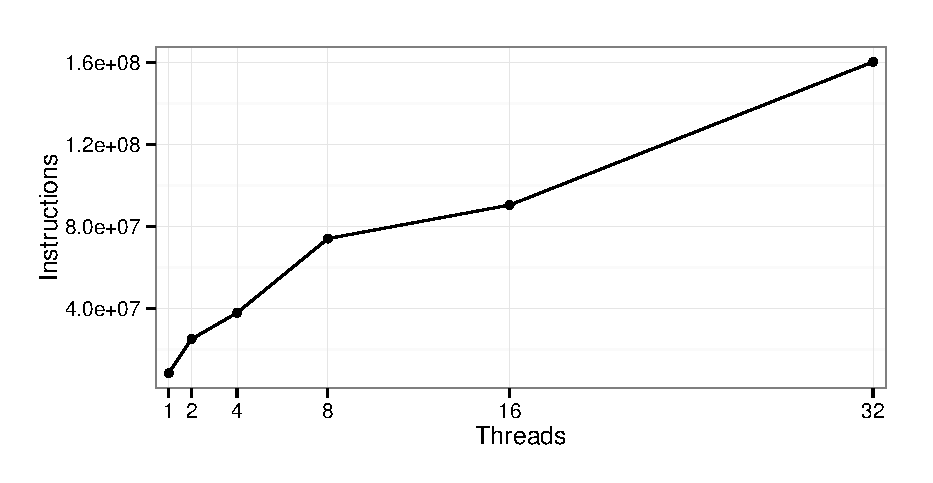
\epsfig{file=figures/parallel/coreutils.eps, width=0.6\columnwidth}
%\caption{Multi-threaded \klee running on \printf from the \coreutils
%suite for five minutes with different numbers of threads.}\label{fig:parallel:coreutils}
%\end{figure}

\section{Evaluation}
\label{sec:par:eval}

We now evaluate the performance of the parallel verification
algorithm. Recall that by design, our verification algorithm has no
false positives --- i.e., if a message trace is declared to be
inconsistent with the sanctioned client software, then it really is.
The only source of false negatives arises from the limited
fidelity of the constraints used to model values returned by
components with which the client software interacts. In these
experiments we make the assumption that the environment modelling is
sound.
We limit our evaluation to \textit{legitimate} message traces since 
our approach is designed to
quickly validate legal behavior in clients that have an unbounded
number of execution paths for exploration.
However, there is no reason that a version of the parallel algorithm 
presented in this \paper could not be applied to the exhaustive
client verification problem from \chref{ch:scv}.

The experiments in this chapter use a multi-threaded version of our
verification tool, built upon KLEE version 1.0\cite{cadar08:klee}, LLVM
3.4\cite{lattner04:llvm} and STP
(rev-940)\cite{ganesh07:stp}.  The experiments were run on system
with 256GB of RAM and 32 3.2GHz processor cores. To evaluate
performance, we applied our parallel algorithm to verify behavior of
legitimate clients of two open-source games from our previous case
studies, namely \xpilot and \tetrinet, which are described in previous
chapters. Evaluation of our parallel verification algorithm requires
message traces for both training and testing.  For \tetrinet, we
generated \tetrinetTraces traces of manual gameplay, each of
\tetrinetTraceLength messages in length (which corresponds to roughly
\tetrinetTraceMins minutes of gameplay).  For \xpilot, we generated
\xpilotTraces traces of manual gameplay, each consisting of
\xpilotTraceLength messages (roughly \xpilotTraceSecs seconds of
gameplay). For our experiments we use the same message traces and
training data from the evaluation section from
\chref{ch:guided}. Note however that these experiments were performed
on a system with a different CPU that has a 10\% higher clock rate.

For each client type, we ran three cross validation experiments over
the message traces with either 1, 8 or 16 worker threads. The training
fragments were clustered with cluster parameter values $\clusters =
\tetrinetFineClusterCount$ and $\clusters = \xpilotFineClusterCount$
for \tetrinet and \xpilot, respectively. These parameters ensured a
single training fragment per cluster and corresponds to the
``default'' configuration used in \chref{ch:guided}. These experiments
do not include results using the ``hint'' configuration, because as we
will see, when using the parallel verification technique, client-side
modification to provide hints to the verifier is not necessary. 
Although the experiments in our evaluation use the same data, the
single worker experiments in this \paper gain the benefits of separate
threads for the \nodeScheduler and \clusterSelector procedures and the
increased clock rate of our experiment platform.

In our evaluation we observe two data points for each \msg{\msgNmbr} in
a message trace, verification \textit{cost} and verification
\textit{delay}. The verification cost for message \msg{\msgNmbr},
denoted \cost{\msgNmbr}, accounts for all time spent in
$\parallelVerifyAlg(\symState{\msgNmbr-1}$, \msg{\msgNmbr},
$\trainingFrags{})$. This is measured as the wall-clock time that
the algorithm takes to determine that \msg{\msgNmbr} is
valid.\footnote{If backtracking occurs, that time is included in the
verification time of the associated message index, i.e., the verification time
for \msg{\msgNmbr} may include the total wall clock time of more than
one instance of $\parallelVerifyAlg$.} Note that the verification time
represents work done concurrently and doesn't represent the total
summation of CPU time across multiple cores. Our second data point
for evaluation is the verification \textit{delay}, which is the delay
in time between the arrival of message \msg{\msgNmbr} at the server
(where a server-to-client message ``arrives'' when it is sent) and the
discovery of an execution prefix \execPrefix{\msgNmbr} that is
consistent with \msg{0}, $\ldots$, \msg{\msgNmbr}.  Delay differs from
verification time by representing the fact that verification for
\msg{\msgNmbr} cannot begin until after verification for \msg{\msgNmbr-1}
completes.  The methods for calculating verification cost and delay
are formally defined in \secref{sec:guided:eval} of \chref{ch:guided}.

\subsection{Case Study: \tetrinet}

\begin{figure}[ht]
\centering
\small
\begin{tabular}{|r|rrr|rrr|}
\hline
& \multicolumn{3}{c|}{Cost (s)} & \multicolumn{3}{c|}{Delay (s)} \\
\hline
\workerCount & 16 & 8 & 1 & 16 & 8 & 1 \\ 
\hline
% & ed-16\_Time & ed-8\_Time & ed-1\_Time & ed-16\_Delay & ed-8\_Delay & ed-1\_Delay \\ 
Min       & 0.0007  & 0.0003  & 0.0001   & 0.0008  & 0.0003  & 0.0001 \\
Max       & 12.1548 & 16.6219 & 100.8736 & 13.1708 & 22.7357 & 337.01 \\
Median    & 0.0368  & 0.0370  & 0.0321   & 0.0489  & 0.0484  & 17.946 \\
Mean      & 0.1287  & 0.1622  & 1.5859   & 0.3975  & 0.6361  & 57.137 \\
%Variance & 0.5796  & 1.0747  & 79.0533  & 2.2025  & 5.4354  & 6040.1192 \\
Std. Dev. & 0.7613  & 1.0367  & 8.8912   & 1.4841  & 2.3314  & 77.718 \\
\hline
\end{tabular}
\caption{Summary statistics for \tetrinet results
\label{fig:tetrinet:parallel:stats}}
\end{figure}

\figref{fig:tetrinet:parallel:stats} shows summary statistics for the
parallel verification algorithm on the \tetrinet experiments and shows
both verification costs and delays for 16-worker, 8-worker and
1-worker configurations.
These results  were obtained by a \tetrinetTraces-fold cross
validation of the \tetrinet traces; i.e., in each test, one of the
traces was selected for testing, and the remainder were used for
training. Each row in \figref{fig:tetrinet:parallel:stats}
is a measure of values (costs or delays) observed over all \tetrinetTraces
experiments.
The mean verification cost per message, regardless of the
number of threads used, is easily beneath the inter-message delay of
roughly \tetrinetInterMessageDelay. As an optimization over results in
\chref{ch:guided}, we can see that parallelization of the verification
algorithm allows us to drop the mean verification cost from
$1.59\secs$ using a single worker thread to $130\msecs$ when using the 16-thread
configuration. If the verifier was placed in-line, this might be an
acceptable overhead on average to add to the processing of network data. However
the maximum verification time of $12.15\secs$ is greater than
the average inter-message delay of \tetrinetInterMessageDelay and
would not be an acceptable amount of latency to add to the
client-server communication. Looking at the Delay columns in
\figref{fig:tetrinet:parallel:stats} we can see that the max delay is
25X less in the 16-worker configuration than in the 1-worker
configuration.

\figref{fig:tetrinet:parallel:time} shows the distribution of
verification cost per message, binned into ten-message bins, across
all \tetrinetTraces traces.  The boxplot labeled ``0'' shows the
distribution of verification times for messages
$\msg{0},\ldots,\msg{9}$ in the \tetrinetTraces traces. In each
boxplot, the ``box'' shows the first, second (median) and third
quartiles, and with whiskers extending to $\pm 1.5$ times the
interquartile range.  Additional outlier points are shown as dots.
Overlaid on each boxplot is a diamond ($\Diamond$) that shows the
average of the data points. In \figref{fig:tetrinet:parallel:time} we can see how additional
worker threads reduce the verification costs. We can also see that it
is the outlier points that dominate the overall time spent in the
verifier, with bands at $90\secs$, $14\secs$ and $10\secs$ for the
three configurations.
Comparing the 1-worker and 16-worker configurations, the performance
multiplier is roughly 9, rather than 16. Our implementation does not
achieve a ``perfect'' speed-up when adding additional workers and
there are several factors that may be at play.
First, a single outlier can represent
verification in multiple node trees due to backtracking. 
Although $2.5\%$ of \tetrinet messages required backtracking, there
is not a direct correlation between existence of backtracking and
higher verification cost. Nevertheless, a round with backtracking cannot
exploit multiple workers as efficiently as possible because early in
the exploration of a node tree because there are more fewer live nodes than
workers available. Second, there is some overhead in our
implementation and as we add more threads there is a added cost to
access shared resources. We attempted to minimize this as much as
possible in our design. 

\figref{fig:tetrinet:parallel:delay} plots the distributions of
per-message verification \textit{delay} between the arrival of message
\msg{\msgNmbr} at the server and the discovery of an execution prefix
\execPrefix{\msgNmbr} that is consistent with \msg{0}, $\ldots$,
\msg{\msgNmbr}.  Delay (\figref{fig:tetrinet:parallel:delay}) differs
from verification cost (\figref{fig:tetrinet:parallel:time}) by
representing the fact that verification for \msg{\msgNmbr} cannot
begin until after that for \msg{\msgNmbr-1} completes.  So, for
example, the rightmost boxplot in each graph provides insight into how
long after the completion of the message trace (in real time) that it
took for verification for the whole trace to complete. We note that
for the multi worker configurations of 8 and 16 workers, verification
is able to keep pace with gameplay and never accumulates delay over
the course of verification. The median of the rightmost boxplot is
virtually zero. Even if verification falls behind at some point in the
game, it always catches up because of the gap between message arrival
times. This indicates that the verifier needs only a fixed sized
buffer of network messages to manage a long-running verification
session. We see that in \figref{fig:tetrinet:parallel:delay}{c}, which
shows the single worker configuration, verification delay lags behind
message arrival times by more than $60\secs$ by the end of a
\tetrinetTraceLength-message trace in the average case. 

\clearpage
\begin{figure}[th]
\centering
\begin{tabular}{c}
%\subfigure[][16 worker threads, $\clusters = \tetrinetFineClusterCount$]{
\subfigure[][$\workerCount = 16$]{
\label{fig:tetrinet:time:parallel_16_default_fine}
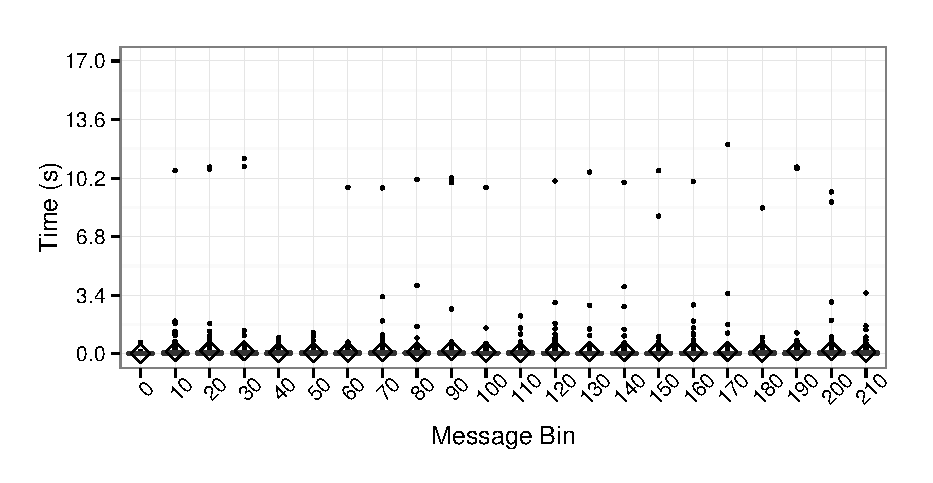
\epsfig{file=figures/parallel/tetrinet_ed-16_Time_boxplot_bar_alt.eps,width=0.6\columnwidth}
} \\[-5pt]
%\subfigure[][8 worker threads, $\clusters = \tetrinetFineClusterCount$]{
\subfigure[][$\workerCount = 8$]{
\label{fig:tetrinet:time:parallel_8_default_fine}
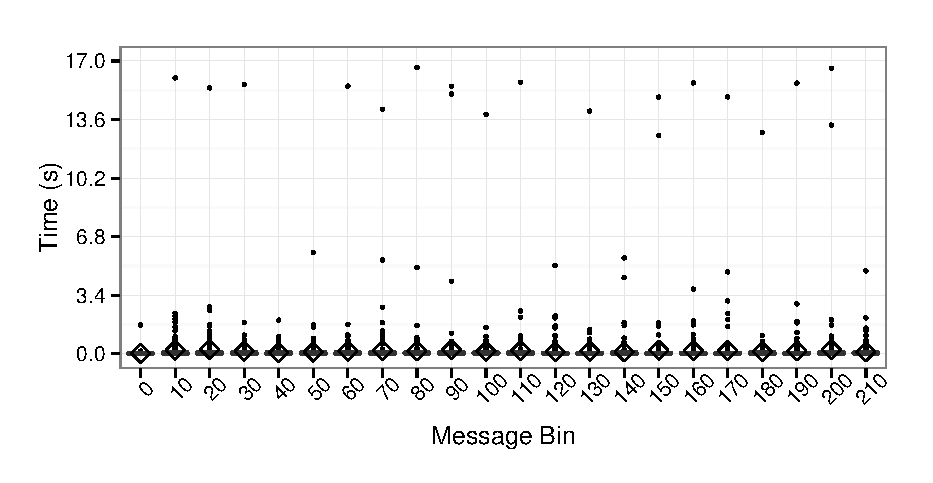
\epsfig{file=figures/parallel/tetrinet_ed-8_Time_boxplot_bar_alt.eps,width=0.6\columnwidth}
} \\[-5pt]
%\subfigure[][1 worker thread, $\clusters = \tetrinetFineClusterCount$]{
\subfigure[][$\workerCount = 1$]{
\label{fig:tetrinet:time:parallel_1_default_fine}
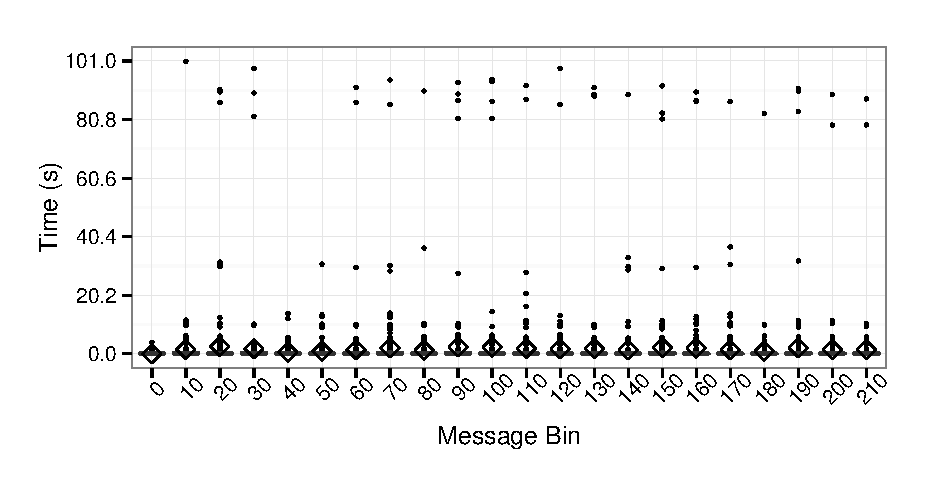
\epsfig{file=figures/parallel/tetrinet_ed-1_Time_boxplot_bar_alt.eps,width=0.6\columnwidth}
}\end{tabular}
\caption[\tetrinet parallel verification costs.]{\tetrinet parallel verification costs.
Cross-validation over \tetrinetTraces traces.  Boxplot at \xval shows
verification costs for messages \msg{\xval}, $\ldots$, \msg{\xval+9}
in each trace (after training on the other traces).  ``$\Diamond$''
shows the average.}
\label{fig:tetrinet:parallel:time}
\end{figure}
\clearpage

\clearpage
\begin{figure}[th]
\centering
\begin{tabular}{c}
%\subfigure[][16 threads, $\clusters = \tetrinetFineClusterCount$]{
\subfigure[][$\workerCount = 16$]{ 
\label{fig:tetrinet:delay:parallel_16_default_fine}
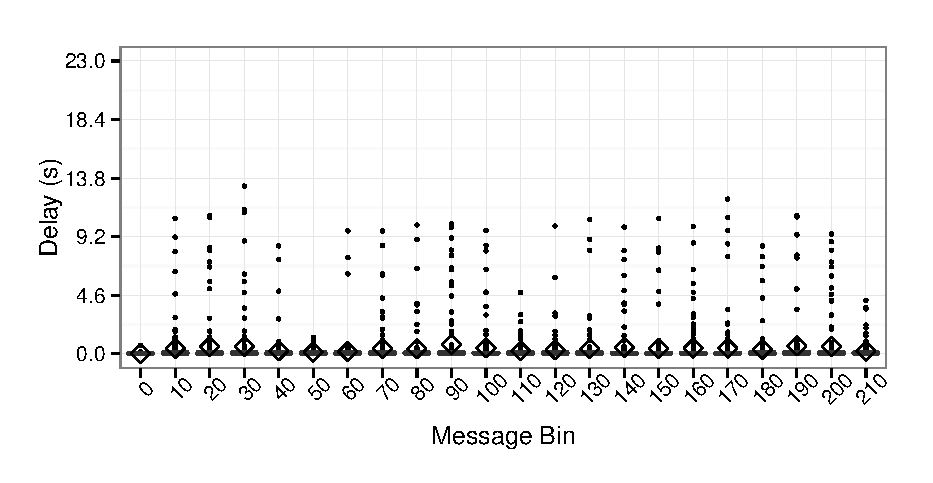
\epsfig{file=figures/parallel/tetrinet_ed-16_Delay_boxplot_bar_alt.eps,width=0.6\columnwidth}
} \\[-5pt]
%\subfigure[][8 threads, $\clusters = \tetrinetFineClusterCount$]{
\subfigure[][$\workerCount = 8$]{
\label{fig:tetrinet:delay:parallel_8_default_fine}
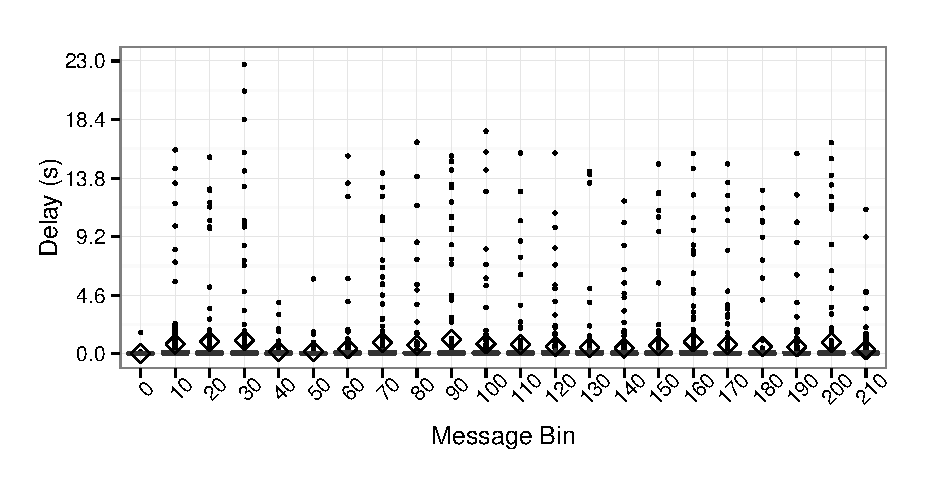
\epsfig{file=figures/parallel/tetrinet_ed-8_Delay_boxplot_bar_alt.eps,width=0.6\columnwidth}
} \\[-5pt]
%\subfigure[][Single-threaded, $\clusters = \tetrinetFineClusterCount$]{
\subfigure[][$\workerCount = 1$]{
\label{fig:tetrinet:delay:parallel_1_default_fine}
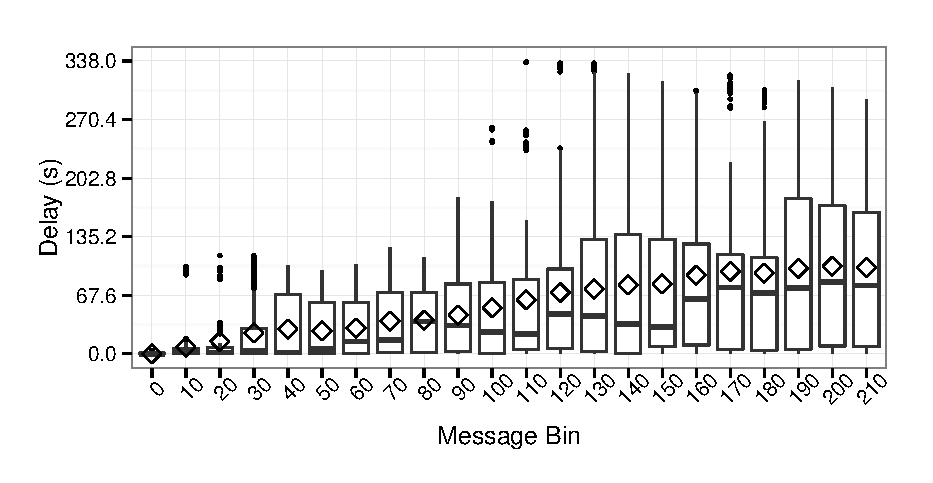
\epsfig{file=figures/parallel/tetrinet_ed-1_Delay_boxplot_bar_alt.eps,width=0.6\columnwidth}
}\end{tabular}
\caption[\tetrinet parallel verification delays.]{\tetrinet parallel verification delays.
Cross-validation over \tetrinetTraces traces.  Boxplot at \xval shows
verification delays for messages \msg{\xval}, $\ldots$, \msg{\xval+9}
in each trace (after training on the other traces).  ``$\Diamond$''
shows the average.}
\label{fig:tetrinet:parallel:delay}
\end{figure}
\clearpage

\subsection{Case Study: \xpilot}

\begin{figure}[ht]
\centering
\small
\begin{tabular}{|r|rrr|rrr|}
\hline
& \multicolumn{3}{c|}{Cost (s)} & \multicolumn{3}{c|}{Delay (s)} \\
\hline
\workerCount & 16 & 8 & 1 & 16 & 8 & 1 \\ 
%& ed-16\_Time & ed-8\_Time & ed-1\_Time & ed-16\_Delay & ed-8\_Delay & ed-1\_Delay \\ 
\hline
Min        & 0.0004 & 0.0004 & 0.0001 & 0.0025 & 0.0022 & 0.0023 \\
Max        & 0.7071 & 0.4966 & 5.4948 & 1.1990 & 1.5294 & 122.85 \\
Median     & 0.0164 & 0.0168 & 0.0122 & 0.0205 & 0.0250 & 29.869 \\
Mean       & 0.0205 & 0.0213 & 0.0658 & 0.0754 & 0.0791 & 32.740 \\
%Variance  & 0.0006 & 0.0004 & 0.0186 & 0.0173 & 0.0156 & 585.0364 \\
Std. Dev.  & 0.0237 & 0.0198 & 0.1364 & 0.1313 & 0.1248 & 24.187 \\
\hline
\end{tabular}
\caption{Summary statistics for \xpilot results
\label{fig:xpilot:parallel:stats}}
\end{figure}


\figref{fig:xpilot:parallel:stats} shows the summary statistics of
the experiments on \xpilot, for verification cost and delay -- 
using 16-worker, 8-worker and 1-worker configurations.
\xpilot poses a different challenge than \tetrinet for verification 
because the message rate is so fast. The tests described here use an \xpilot
configuration that resulted in an average of \xpilotMsgsPerSec
messages per second or an average inter-message
time of \xpilotInterMessageDelay. Nevertheless, with our parallel
verification technique, we can achieve a mean verification
cost of only $20\msecs$ and return a verification result in less
than $0.71\secs$ for all messages in our experiments. 
The multi-worker configurations are both more than $3\times$ faster
on average than the single worker configuration.
For the 16-worker configuration, the verifier is on average
only $75\msecs$ behind ($1.19\secs$ in the worst case), whereas when
using only a single-worker, verification delay is on average
$32.7\secs$ and over 2 minutes in the worst case.
These results demonstrate that in-line verification is feasible
and would add minimal latency in the average case. However,
adding $1.19\secs$ of latency in the worst case would not be acceptable
for fast-paced gameplay.

In \figref{fig:xpilot:parallel:time}, the verification costs for
\xpilot are shown for the three worker configurations across the
message traces. Each boxplot in \figref{fig:xpilot:parallel:time}
represents $100 \times \xpilotTraces$ points.
Despite a mean verification cost of $75\msecs$ when using
a single worker thread, the fast pace of \xpilot makes it difficult 
for verification to keep pace with the game.  This effect is shown in
\figrefi{fig:xpilot:parallel:delay}{c}.  
However, by increasing the number of worker threads, we can see that
in the 16-worker and 8-worker configurations, verification delay
never significantly falls behind and could use only a fixed
buffer of messages for verification in long running sessions.

\clearpage
\begin{figure}[th]
\centering
\begin{tabular}{c}
%\subfigure[][16 threads, $\clusters = \xpilotFineClusterCount$]{
\subfigure[][$\workerCount = 16$]{
\label{fig:xpilot:time:parallel_16_default_fine}
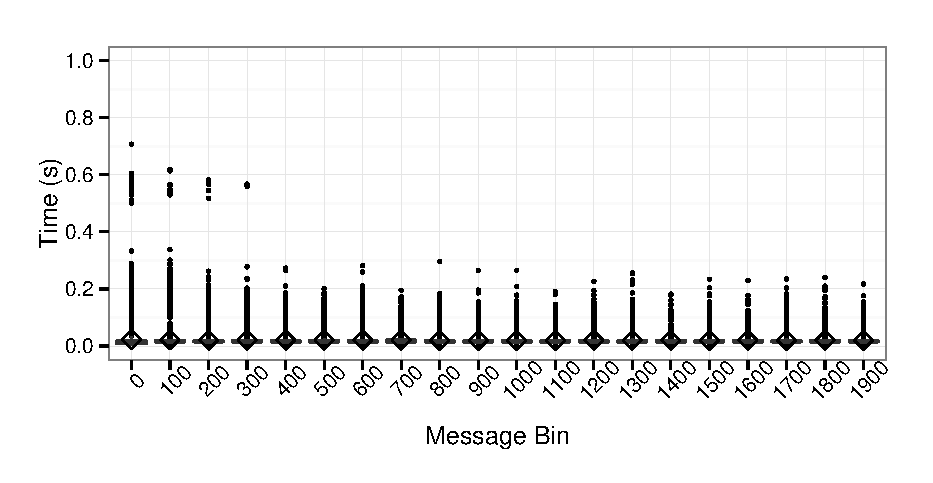
\epsfig{file=figures/parallel/xpilot_ed-16_Time_boxplot_bar_alt.eps,width=0.6\columnwidth}
} \\[-5pt]
%\subfigure[][8 threads, $\clusters = \xpilotFineClusterCount$]{
\subfigure[][$\workerCount = 8$]{
\label{fig:xpilot:time:parallel_8_default_fine}
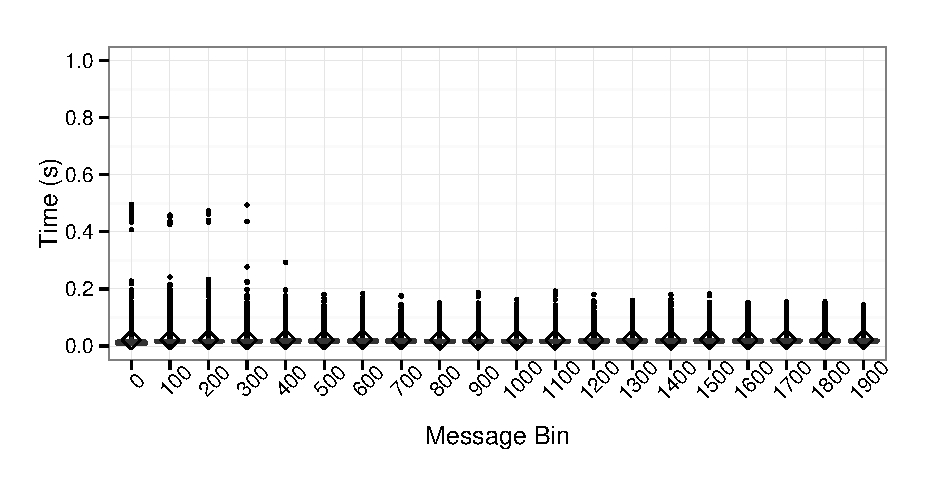
\epsfig{file=figures/parallel/xpilot_ed-8_Time_boxplot_bar_alt.eps,width=0.6\columnwidth}
} \\[-5pt]
%\subfigure[][Single-threaded, $\clusters = \xpilotFineClusterCount$]{
\subfigure[][$\workerCount = 1$]{
\label{fig:xpilot:time:parallel_1_default_fine}
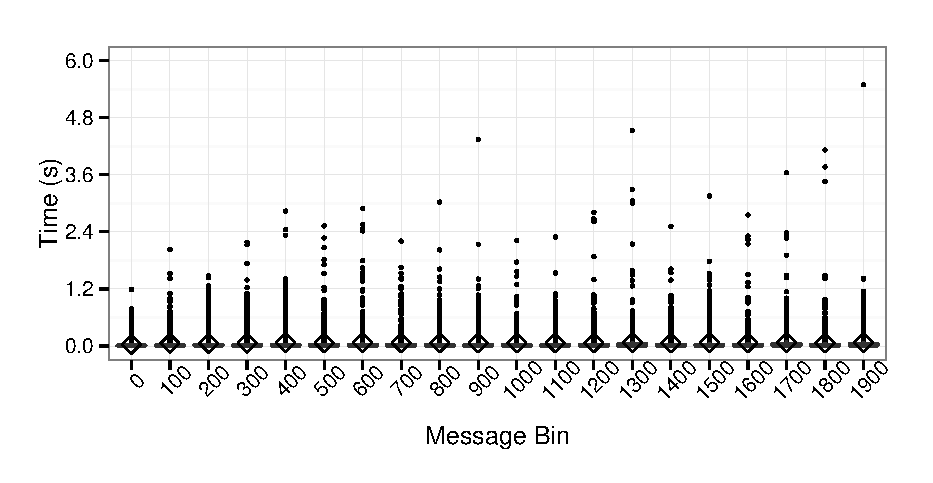
\epsfig{file=figures/parallel/xpilot_ed-1_Time_boxplot_bar_alt.eps,width=0.6\columnwidth}
}
\end{tabular}
\caption[\xpilot parallel verification costs]{\xpilot parallel
  verification costs.
Cross-validation over \xpilotTraces traces.  Boxplot at \xval shows
verification costs for messages \msg{\xval}, $\ldots$, \msg{\xval+99}
in each trace (after training on the other traces).  ``$\Diamond$''
shows the average.}
\label{fig:xpilot:parallel:time}
\end{figure}
\clearpage

\clearpage
\begin{figure}[th]
\centering
\begin{tabular}{c}
%\subfigure[][16 threads, $\clusters = \xpilotFineClusterCount$]{
\subfigure[][$\workerCount = 16$]{
\label{fig:xpilot:delay:parallel_16_default_fine}
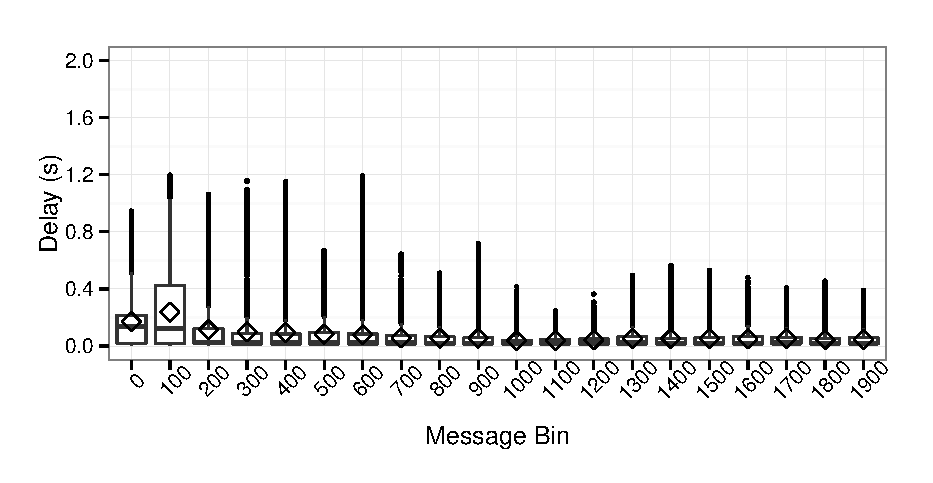
\epsfig{file=figures/parallel/xpilot_ed-16_Delay_boxplot_bar_alt.eps,width=0.6\columnwidth}
} \\[-5pt]
%\subfigure[][8 threads, $\clusters = \xpilotFineClusterCount$]{
\subfigure[][$\workerCount = 8$]{
\label{fig:xpilot:delay:parallel_8_default_fine}
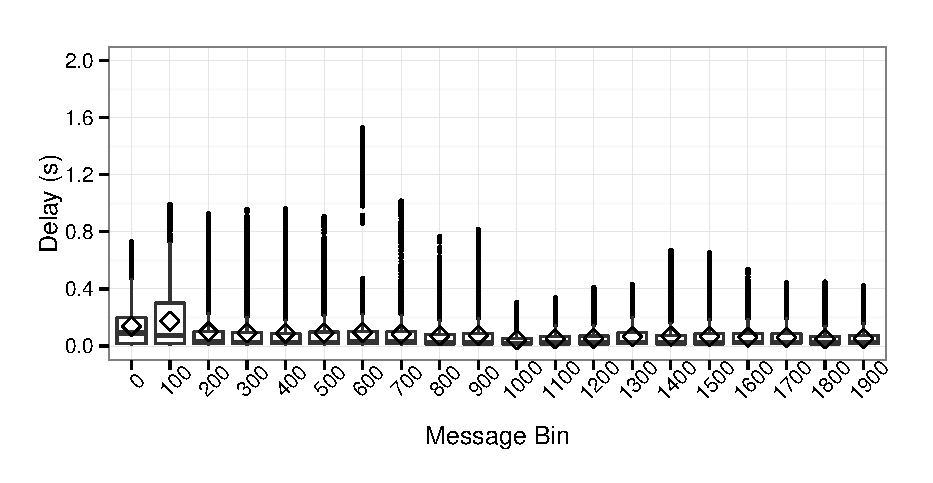
\epsfig{file=figures/parallel/xpilot_ed-8_Delay_boxplot_bar_alt.eps,width=0.6\columnwidth}
} \\[-5pt]
%\subfigure[][Single-threaded, $\clusters = \xpilotFineClusterCount$]{
\subfigure[][$\workerCount = 1$]{
\label{fig:xpilot:delay:parallel_1_default_fine}
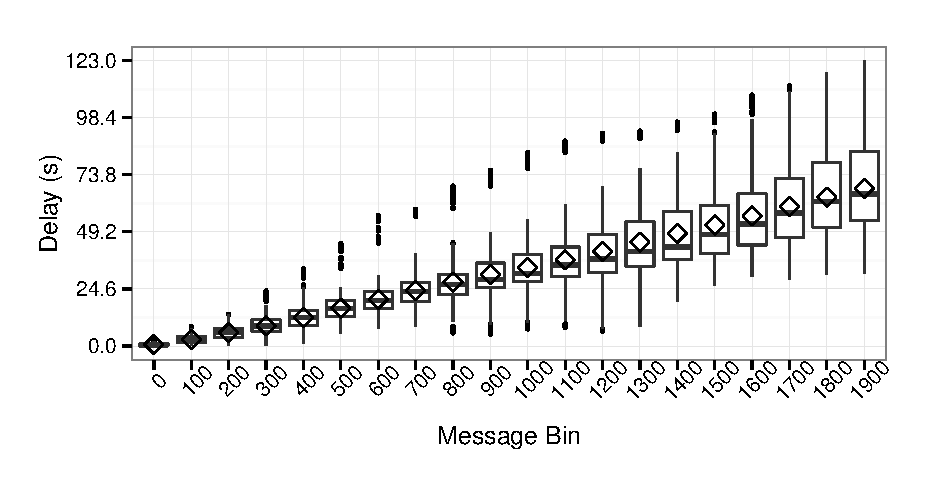
\epsfig{file=figures/parallel/xpilot_ed-1_Delay_boxplot_bar_alt.eps,width=0.6\columnwidth}
}
\end{tabular}
\caption[\xpilot parallel verification delays]{\xpilot parallel
  verification delays.
Cross-validation over \xpilotTraces traces.  Boxplot at \xval shows
verification delays for messages \msg{\xval}, $\ldots$, \msg{\xval+99}
in each trace (after training on the other traces).  ``$\Diamond$''
shows the average.}
\label{fig:xpilot:parallel:delay}
\end{figure}
\clearpage


\begin{figure}[t]
\centering
\begin{tabular}{c}

{\subfigcapskip = 5pt \subfigure[][$\tetrinet$]{
  \small
\begin{tabular}{|r|r|r|}
 \hline
 \multicolumn{3}{|c|}{Cost(s)} \\
 \hline
& \multicolumn{1}{c|}{with } &\multicolumn{1}{c|}{without } \\
& \multicolumn{1}{c|}{\clusterSelector } &\multicolumn{1}{c|}{\clusterSelector } \\
& \multicolumn{1}{c|}{thread} &\multicolumn{1}{c|}{thread} \\
 \hline
%    & ed-8-async-ed\_Cost & ed-8-no-async-ed\_Cost & \\
Min           & 0.0003  & 0.0003   \\
Max           & 16.0291 & 17.1220  \\
Median        & 0.0349  & 0.0221   \\
Mean          & 0.1804  & 0.1833   \\
Std.Dev.      & 1.0507  & 1.2745   \\
\hline
\end{tabular}
} }\\

{\subfigcapskip = 5pt \subfigure[][$\xpilot$]{
  \small
\begin{tabular}{|r|r|r|}
 \hline
 \multicolumn{3}{|c|}{Cost(s)} \\
 \hline
& \multicolumn{1}{c|}{with } &\multicolumn{1}{c|}{without } \\
& \multicolumn{1}{c|}{\clusterSelector } &\multicolumn{1}{c|}{\clusterSelector } \\
& \multicolumn{1}{c|}{thread} &\multicolumn{1}{c|}{thread} \\
 \hline
%    & ed-8-async-ed\_Cost & ed-8-no-async-ed\_Cost & \\
  Min        & 0.0007 & 0.0006  \\
  Max        & 0.4312 & 0.4469  \\
  Median     & 0.0158 & 0.0157  \\
  Mean       & 0.0170 & 0.0172  \\
  Std.Dev.   & 0.0184 & 0.0182  \\
  \hline
\end{tabular}
} } \\

\end{tabular}
\caption[Verification cost with and without \clusterSelector thread]
{Summary of verification cost in seconds for \tetrinet and \xpilot,
with and without a \clusterSelector thread, using $\workerCount = 8$.}
\label{fig:clusterselector}
\end{figure}


\subsection{Evaluation of \nodeScheduler and \clusterSelector Threads}

The parallel algorithm presented in this \paper divides and
distributes the verification computation into separate threads across
multiple CPU cores. Recall in addition to a variable number of
\verifyWorker threads, the algorithm uses two additional threads; one
for the \nodeScheduler procedure (\figref{fig:paralg:sub}) and one for
the \clusterSelector procedure (detailed in \chref{ch:guided}). In this section,
we will examine the performance impact of computing the work done by
the procedures \nodeScheduler and \clusterSelector in separate threads
as opposed to an alternative arrangement where the work is divided
amongst all \verifyWorker threads.

In our current experiments and implementation, the usage of a
\nodeScheduler thread does not provide a measurable performance
benefit. The increased granularity of the workload is offset by the
small overhead of the implementation. Nevertheless, this design
provides a cleaner separation of work for the implementation and we
predict verification of different client software in the future may
benefit from the architecture.

Using a separate thread for the \clusterSelector procedure does
however have a measurable performance impact. The procedure
\clusterSelector is provided a network message \msg{\msgNmbr} and a
set of execution fragments \trainingFrags{}, produced during training
and returns a subset of execution fragments \trainingFrags{\msgNmbr},
used by the \nodeScheduler to inform node selection. The
details of the \clusterSelector algorithm are described in
\chref{ch:guided}.
In our experimental results thus far, each thread has exclusive access
to a CPU core. However, the algorithm is designed so that the
\clusterSelector method can be called synchronously by removing \Spawn
on Line \ref{fig:paralg:spawnClusterSelector} of the
\parallelVerifyAlg procedure in \figref{fig:paralg}. We evaluated this
design decision on the case studies \xpilot and \tetrinet with a new
experimental setup where the \clusterSelector procedure is called
synchronously before the \verifyWorker threads are spawned.
\figref{fig:clusterselector} shows a summary of the verification costs
in seconds for the case studies using $\workerCount = 8$.
The mean verification cost in seconds increases measurably for both
\xpilot and \tetrinet when the verifier is executed without a
\clusterSelector thread.


\section{Evaluation of Optimization Techniques}
\label{sec:par:evalopt}

The performance of parallel symbolic verification is dependent on many
factors. We have shown that a parallel implementation with multiple
worker threads decreases the cost of verification over the
single-threaded implementation outlined in the previous chapters.
Using symbolic execution as the basis for a verification method has
required several optimizations to the underlying implementation, which
have been described in previous chapters. In this section we review
these optimization techniques and evaluate their impact and
interaction with parallel symbolic execution in our case studies.

Several optimization methods were developed and utilized to improve
the performance of symbolic execution for verification. \klee was
designed with techniques for reducing the size and number of queries
that are sent to the underlying constraint solver. One of these
techniques is a cache of solver queries and their respective solver
outputs. Before a constraint formula or query is tested for
satisfiability via \stp, \klee checks a \emph{query cache} and if the
cache contains a hit, the potentially expensive solver operation can
be avoided. If there is a miss, the solver must be instantiated and
the result is added to the cache afterwards. In our implementation,
each worker thread operates a separate solver chain, which means that
\klee query caches are not shared between workers. Additionally,  the
caches are empty upon starting verification of a message sequence. In
the previous chapters, two methods have been demonstrated that enable
better utilization of these caches:
canonicalization~(\secref{sec:guided:eval:results:tetrinet}) and
constraint pruning~(\secref{ssec:scv:approach:pruning}). The
canonicalization method is used to rewrite the variable names in a
solver query before the query cache is checked. The constraint pruning
optimization is used to eliminate variables and formula constructs
that have not been concretized but can be shown to never be relevant
to future branch conditions; variables can be pruned that are no
longer in the scope of execution and are independent from the current
scope.

In this section we evaluate the impact and interactions of parallel
symbolic verification with and without the canonicalization and
constraint pruning optimizations. The experiment operates with
the verifier in three configurations.
The first configuration, which we call \allopt,
is the same configuration used in~\secref{sec:par:eval}, and utilizes
both canonicalization and constraint pruning. The second
configuration, \nocanon, is the same as the former but disables the
canonicalization of queries before the query cache is checked. The
third and final configuration, \noprune, is the same as \allopt
but with constraint pruning disabled. Additionally, we are only
verifying a \emph{single} game play log from each of our case studies,
\xpilot and \tetrinet. Despite using a single log,
the experimental results are representative of
the full case study data sets. The use of a single log
allows easier characterization of the interactions of the optimizations with
symbolic client verification. All of the experiments were performed
with $\workerCount = 16$. If the experiments are configured with
$\workerCount = 1$, disabling canonicalization or constraint pruning
causes the verification to take several hours. In addition to
demonstrating the benefit of constraint pruning and canonicalization,
these results are also useful to characterize the workloads of our
case studies in terms of the symbolic execution optimizations of \klee
and may be of use to others.

\subsection{Impact of Optimizations on Cost and Delay}

\begin{figure}[th]
\centering
{\subfigcapskip = 5pt \subtable[][$\tetrinet$]{
\small
\begin{tabular}{|r|rrr|rrr|}
\hline
& \multicolumn{3}{c|}{Cost (s)}& \multicolumn{3}{c|}{Delay (s)} \\
\hline
& \allopt & \nocanon & \noprune & \allopt & \nocanon & \noprune \\
\hline
Min      & 0.0016 & 0.0014 & 0.0013 & 0.0016 & 0.0014 & 0.0013  \\
Max      & 1.4875 & 3.3591 & 4.7334 & 1.4925 & 3.3690 & 4.7390  \\
Median   & 0.0384 & 0.0376 & 0.0760 & 0.0504 & 0.0467 & 0.1281  \\
Mean     & 0.0835 & 0.0986 & 0.2214 & 0.1387 & 0.1919 & 0.4207  \\
Std. Dev.& 0.1970 & 0.3225 & 0.5242 & 0.2655 & 0.5062 & 0.7522  \\
\hline
\end{tabular}
\label{par:singlecostdelay:tetrinet}
} } \\

{\subfigcapskip = 5pt \subfigure[][$\xpilot$]{
\small
\begin{tabular}{|r|rrr|rrr|}
\hline
& \multicolumn{3}{c|}{Cost (s)}& \multicolumn{3}{c|}{Delay (s)} \\
\hline
& \allopt & \nocanon & \noprune & \allopt & \nocanon & \noprune \\
\hline
Min      & 0.0009 & 0.0007 & 0.0009 & 0.0027 & 0.0086  & 0.0090    \\
Max      & 0.6268 & 0.7627 & 8.2392 & 1.1417 & 55.0549 & 1158.8995 \\
Median   & 0.0171 & 0.0327 & 0.3217 & 0.0266 & 35.5776 & 421.1561  \\
Mean     & 0.0198 & 0.0559 & 0.6080 & 0.1084 & 29.5545 & 537.8276  \\
Std. Dev.& 0.0256 & 0.1213 & 0.7888 & 0.2019 & 16.8834 & 410.7422  \\
\hline
\end{tabular}
\label{par:singlecostdelay:xpilot}
} } \\
\caption{Verification costs and delays for \tetrinet and \xpilot for a
single representative log.}
\label{par:singlecostdelay}
\end{figure}

We now examine the performance interactions of canonicalization and
constraint pruning with parallel symbolic verification. We start with
an experiment to determine the impact of these optimizations on our key
evaluation metrics, cost and delay. \figref{par:singlecostdelay} shows
an overview of the cost and delay times per message during the
verification of a single game play trace from the \tetrinet and
\xpilot case studies. In \figref{par:singlecostdelay:tetrinet} we can
see that for \tetrinet, either disabling the canonicalization
optimization (\nocanon) or disabling the constraint pruning optimization (\noprune)
adversely affects the mean values for cost and delay. The
benefit of these optimizations is even more prevalent in the \xpilot
results shown in \figref{par:singlecostdelay:xpilot}. Disabling
canonicalization increases the mean verification cost by a factor of
five and due to the rapid rate at which \xpilot messages are
transmitted, disabling canonicalization introduces more than a $200
\times$ increase in the mean verification delay. Also, for \xpilot,
constraint pruning is even more important for efficient verification;
the mean verification delay increases from roughly a $0.10$ seconds
with all optimizations to over $8$ minutes without constraint pruning.

\subsection{Impact of Optimizations on Solver Queries}

We can better understand how the canonicalization and constraint
pruning  optimizations impact cost and delay in parallel symbolic
verification by looking at how these optimizations change the
properties of the formulas sent as queries to the constraint solver
(\stp).

\subsubsection{Query Cache Hit Rate}
\figref{par:cachehitrates} shows the overall hit rates of the query
cache in the single log verification experiment and can begin to
explain why the optimizations make verification more efficient.
With all optimizations (\allopt), both \tetrinet and
\xpilot have high hit rates of 99.89\% and 97.13\% respectively. In
other words, of all queries to the constraint solver stack, less than
0.12\% and 3.87\% (\tetrinet and \xpilot, respectively) actually
result in a potentially expensive call to to the constraint solver
\stp. Without the canonicalization optimization (\nocanon), the
effectiveness of the cache is reduced significantly for \tetrinet and
even more so for \xpilot, dropping the hit rate to 33.26\%.

\begin{figure}[t]
\centering
\begin{tabular}{|r|r|r|}
\hline
         & \tetrinet & \xpilot \\
\hline
\allopt  & 0.9989 & 0.9713 \\
\nocanon & 0.6860 & 0.3326 \\
\noprune & 0.9989 & 0.9618 \\
\hline
\end{tabular}
\caption{Overall query cache hit rates for a single log selected from
each of the \tetrinet and \xpilot case studies.}
\label{par:cachehitrates}
\end{figure}

Canonicalization has a large impact on the query cache hit rate
because it reduces the space of variable names that can be found in
the constraint cache. During verification, when a symbolic variable is
generated (e.g., to represent an unknown user input value), in
addition to representing a region of memory, the variable is given a
unique name. The symbolic variable name may be used in a formula to
represent any constraints on any associated symbolic memory region.
Verification in our case studies often generates constraints that have
the same formula structure, but with different variable names. By
canonicalizing the variable names before the query cache is utilized,
the chance of a cache hit becomes much more likely and the expensive
constraint solver query can be avoided. The need for canonicalization highlights a
key difference between the use of symbolic execution for client
verification versus more traditional uses of symbolic execution;
client verification exercises the same paths repeatedly but with
slightly different contexts. Unlike canonicalization, constraint
pruning does not significantly improve the cache hit rate for the case
studies; the \noprune experiment shows the same hit rate for \tetrinet
and only slightly lower hit rate for \xpilot.

\begin{figure}[th]
\centering
\begin{tabular}{c}
\subfigure[][$\tetrinet$]{
\label{par:cachehitratepermessage:tetrinet}
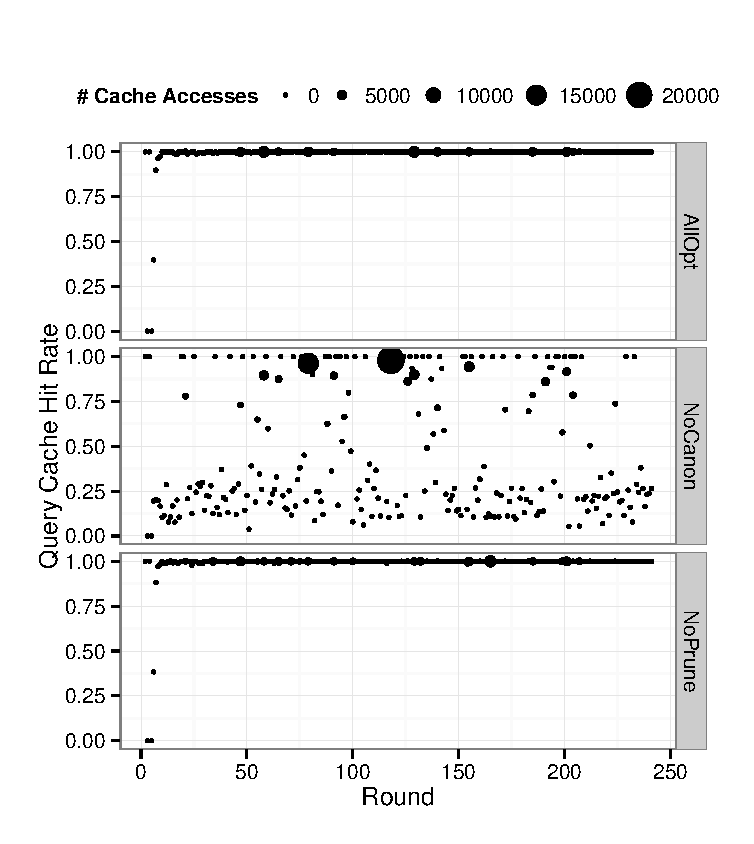
\epsfig{file=figures/parallel/RoundNumbervsQueryCacheHitRate_tetrinet_point_grid_group.eps,width=0.45\columnwidth}
}
\subfigure[][$\xpilot$]{
\label{par:cachehitratepermessage:xpilot}
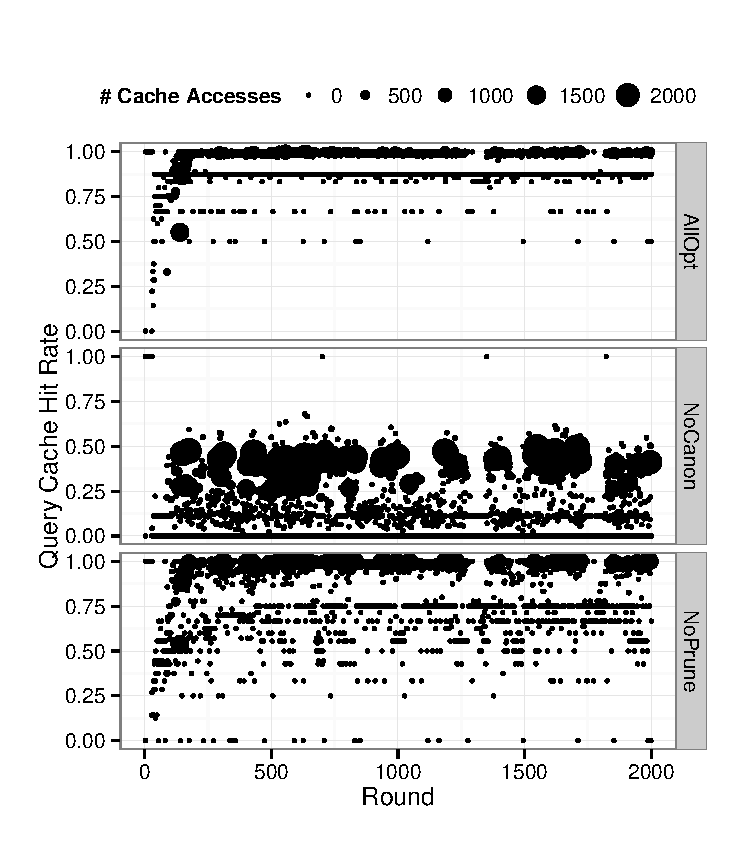
\epsfig{file=figures/parallel/RoundNumbervsQueryCacheHitRate_xpilot_point_grid_group.eps,width=0.45\columnwidth}
}
\end{tabular}
\caption[Query Cache Hit Rates.]{
Query cache hit rates per message for the verification of a single
representative game play log from each of the case studies.
The area of each circle is scaled relative to the
number of cache accesses represented.}
\label{par:cachehitratepermessage}
\end{figure}


\subsubsection{Query Cache Hit Rate Per Message}
\figref{par:cachehitratepermessage} shows the same cache hit rate
values shown in \figref{par:cachehitrates} but \emph{per message}.
\figref{par:cachehitratepermessage} illustrates the change in the
query cache hit rate as verification progresses through the message
log as well as the volume of cache accesses needed to verify each
message. The query cache hit rate is shown on the y-axis and the
message index on the x-axis. Each plotted dot represents the effective
hit rate of the query cache over all queries during the creation of
\execPrefix{\msgNmbr} from \execPrefix{\msgNmbr-1}. The number of
cache accesses needed to construct each \execPrefix{\msgNmbr} is
represented exactly by the area of each circle. The legend shows
several example circle areas and the corresponding number of cache
accesses each area represents. The three configuration types are
indicated on the right side of each plot.

\figref{par:cachehitratepermessage:tetrinet} shows the \tetrinet
experiment. The \allopt and \noprune results are very similar; after
verification of a few messages, the query cache contains enough
entries to produce a very high cache hit rate. However for the
\nocanon configuration, we can observe that without canonicalization
the query cache does not contain entries that match the formulas with
new variables names and is not effective, even towards the end of the
message log.

The \xpilot results are shown in
\figref{par:cachehitratepermessage:xpilot}. The \allopt configuration
for \xpilot shows that verification proceeds for around 30 messages
before the cache hit rate improves significantly. The \noprune
configuration is similar, but with intermittent poor performance due
to the disabling of constraint pruning. Additionally, noticeable bands
appear in the results because of the variety of message types. The
\nocanon plot for \xpilot shows the significance of the
canonicalization optimization, both the query cache hit rate and the
volume of cache accesses are affected with negative impacts on
performance.

\begin{figure}[th]
\centering
\begin{tabular}{c}
\subfigure[][$\tetrinet$]{
\label{par:cachehitcount:tetrinet}
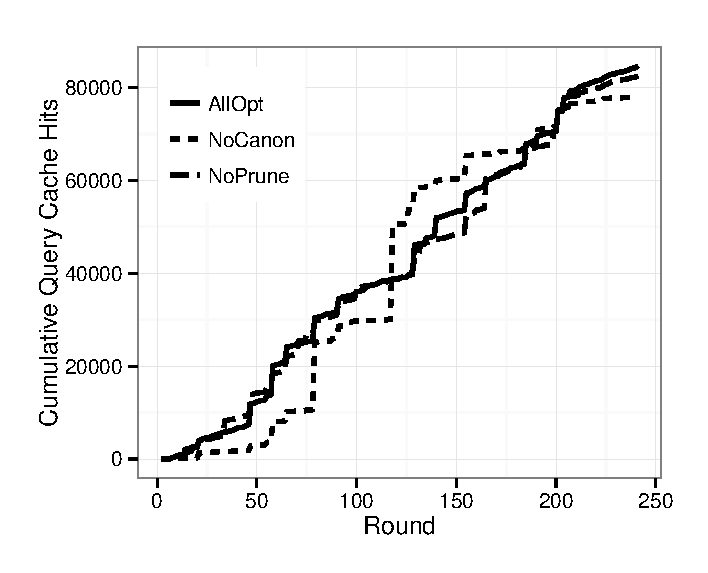
\epsfig{file=figures/parallel/RoundNumbervsCumQueryCacheHits_tetrinet_line_group.eps,width=0.45\columnwidth}
}
\subfigure[][$\xpilot$]{
\label{par:cachehitcount:xpilot}
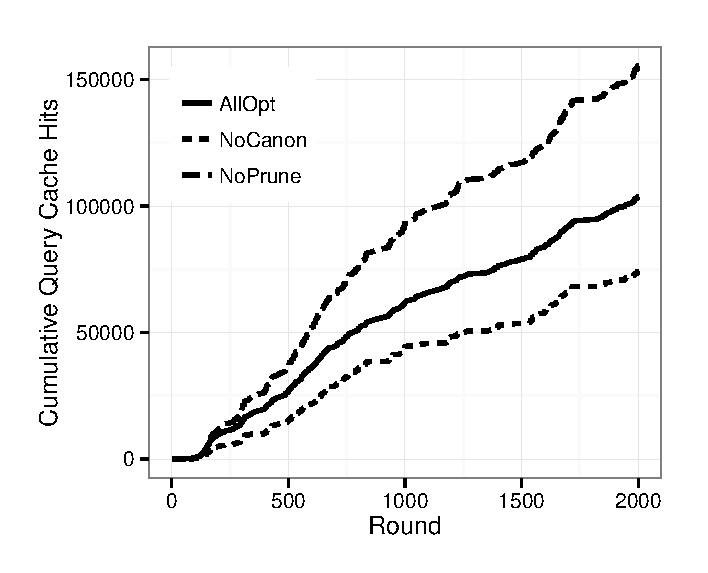
\epsfig{file=figures/parallel/RoundNumbervsCumQueryCacheHits_xpilot_line_group.eps,width=0.45\columnwidth}
}
\end{tabular}
\caption[Cumulative number of cache hits.]{The cumulative number query cache hits over the verification
of a single game play log from \xpilot and \tetrinet.}
\label{par:cachehitcount}
\end{figure}

\subsubsection{Cumulative Query Cache Hits and Solver Queries}
We now examine how the query cache is exercised by the three
configurations in terms of the cumulative number of hits in the query
cache and the cumulative number of misses that lead to actual calls to
the constraint solver. \figref{par:cachehitcount} shows the cumulative
number of query cache hits for \tetrinet and \xpilot over the
verification of a single representative game play log.  By the time
the last message is verified, the \tetrinet experiment results in over
$80,000$ cache hits amongst the 16 worker threads, while the  \xpilot
experiment generates over $100,000$ cache hits. The cumulative number
of final cache hits is about the same for each configuration of
\tetrinet. However for \xpilot there is a significant difference; the
\noprune configuration has approximately twice as many query cache
hits as \nocanon. The \noprune configuration produced more cache hits
overall, even more than \allopt, because the overall search was less
efficient and interacted with the parallel verification.
Under \noprune, each verify worker has a more complex
workload with larger constraints and therefore the time to discover
the correct execution prefix increases. The additional time needed allows
other worker threads to search additional paths, thus increasing the
number of query cache hits. This aligns with the results for the
\noprune configuration in \figref{par:cachehitratepermessage:xpilot};
the relative query cache hit rate is slightly less than \allopt, but
the overall number of cache accesses (indicated by the size of the
circles) is larger.

\begin{figure}[th]
\centering
\begin{tabular}{c}
\subfigure[][$\tetrinet$]{
\label{par:solverqueries:tetrinet}
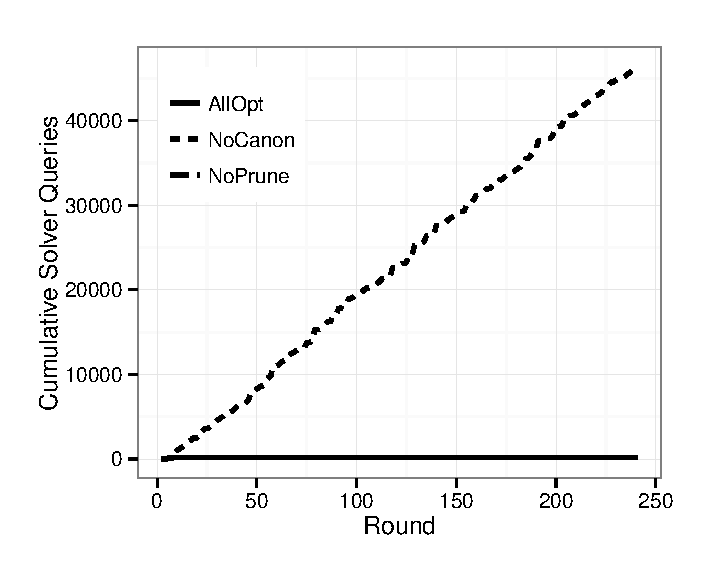
\epsfig{file=figures/parallel/RoundNumbervsCumQueries_tetrinet_line_group.eps,width=0.45\columnwidth}
} %\\[-5pt]
\subfigure[][$\xpilot$]{
\label{par:solverqueries:xpilot}
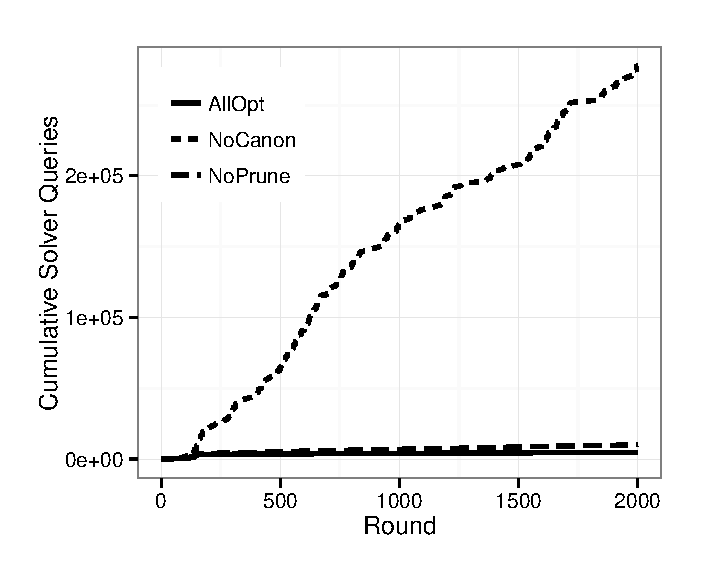
\epsfig{file=figures/parallel/RoundNumbervsCumQueries_xpilot_line_group.eps,width=0.45\columnwidth}
} %\\[-5pt]
\end{tabular}
\caption[Cumulative number of solver queries.]{The cumulative number
  of queries to the solver (\stp) over the verification of a single game play log
from \xpilot and \tetrinet.}
\label{par:solverqueries}
\end{figure}

A query is only made to the constraint solver \emph{after} a query
cache miss has occurred. Therefore, the number of misses in the caches
is exactly equal to the number of actual queries made to the
constraint solver. \figref{par:solverqueries} shows the cumulative
number of queries to the constraint solver (\stp) over the
verification of single game log for both \tetrinet and \xpilot using
the three different configurations. Here it is very evident that for
both case studies, the canonicalization optimization significantly
reduces the overall number of expensive queries to \stp. If we combine
the overall numbers for \tetrinet from
\figref{par:solverqueries:tetrinet} and
\figref{par:cachehitcount:tetrinet},
we can see that \nocanon had
a significantly greater number of solver queries, including queries
resulting in a cache hit. Again, this is due to an interaction with
workers operating in parallel; the time to discover a valid execution
prefix increases when more time is spent in the constraint solver.
Therefore, other worker threads explore additional paths, leading to
a greater number of client instructions executed across all worker
threads. The impact of this interaction is examined further in the
next section~ (\ref{sec:par:optinst}).

\begin{figure}[th]
\centering
\begin{tabular}{c}
\subfigure[][$\tetrinet$]{
\label{par:querysize:tetrinet}
\epsfig{file=figures/parallel/RoundNumbervsAverageQueryConstructs_tetrinet_point_grid_group.eps,width=0.45\columnwidth}
}
\subfigure[][$\xpilot$]{
\label{par:querysize:xpilot}
\epsfig{file=figures/parallel/RoundNumbervsAverageQueryConstructs_xpilot_point_grid_group.eps,width=0.45\columnwidth}
}
\end{tabular}
\caption[Complexity of Solver Queries.]{
Average query construct count per message
verified in a single representative game play log from \tetrinet and
\xpilot.
The area of each circle is scaled relative to the
number of solver queries represented.}
\label{par:querysize}
\end{figure}

\subsubsection{Complexity of Solver Queries}
In addition to the number of queries to the constraint solver, we also
characterize the complexity of these queries in terms of the size of
the queried constraint. A constraint formula consists of binary and
unary operators on variables or concrete values; each of those
operators is counted as a single construct. The metric we use for size
is a measure that corresponds to the number constructs in the query.
Each circle plotted in \figref{par:querysize} summarizes the
complexity of the constraint formulas sent to the solver by showing
the average number of constructs in the solver queries during the
creation of \execPrefix{\msgNmbr} from \execPrefix{\msgNmbr-1}.
Additionally, the area of each circle represents the number of
queries sent to the constraint solver. Note that the data shown
in \figref{par:querysize} characterizes the query formulas sent to
the constraint solver (STP) after a query cache miss has occurred.

As we have seen, the lack of canonicalization leads to poor cache
utilization; the effects of which are twofold for the \nocanon
configuration in \figref{par:querysize:tetrinet}. First, the average
query construct count (on the y-axis) is greater than \allopt across
the message sequence. Without canonicalization, fewer
queries are located in the query cache and thus more queries are sent
to the constraint solver and these queries have a greater
query construct count. Second, the total number of
queries is greater (area of circles) because poor cache utilization
leads to a greater number of client instructions executed; this is
examined further in the next section (\ref{sec:par:optinst}).

The \xpilot experiment in \figref{par:querysize:xpilot} reveals
similar results for the \nocanon configuration. The average query
construct count (on the y-axis) is greater than \allopt across the
message sequence because larger queries are not located in the cache
and the total number of queries is larger (area of circles) because a
greater number of client instructions are executed. In the \noprune
configuration, there is a behavior where the average number of
constructs increases with each creation of \execPrefix{\msgNmbr} from
\execPrefix{\msgNmbr-1}, with a periodic ``reset'' of the average
constraint complexity. This behavior is seen when constraint pruning
is disabled because independent constraints that contain symbolic
variables that are generated for \execPrefix{\msgNmbr}, may have a
relationship with a symbolic variable generated during the creation of
\execPrefix{\msgNmbr-1}. For example, suppose a symbolic variable
represents the current time and is fully symbolic. This variable will
be strictly greater than a similar variable that represents an
earlier instance of the time. These constraints do not grow throughout
the entire gameplay session because of high level game events that
cause, for example, a reset of certain game state values. By using the
constraint pruning techniques that are described in the previous
chapter, the complexity of solver queries can be dramatically reduced
and can be seen clearly in \figref{par:querysize:xpilot} by comparing
\allopt and \noprune.

\subsection{Impact of Optimizations on Instructions Executed and Memory Usage}
\label{sec:par:optinst}

%\begin{table}[ht]
%\centering
%\begin{tabular}{rrrr}
%\hline
%% & No-Canonicalization\_InstructionCount & No-Pruning\_InstructionCount & All-Opt\_InstructionCount \\
%               & \nocanon       & \noprune       & \allopt \\
%\hline
%
%Min            & 61.0000        & 61.0000        & 61.0000             \\
%Max            & 77361709.0000  & 26033093.0000  & 23564623.0000       \\
%Median         & 211246.0000    & 276570.0000    & 369236.5000         \\
%Mean           & 1413244.8667   & 1150238.6250   & 1141894.7417        \\
%Std.Dev        & 6630185.9084   & 3160070.1607   & 3323343.5091        \\
%Sum            & \num{3.39e8} & \num{2.76e8} & \num{2.74e8}      \\
%
%%Min            & 61.0000        & 61.0000        & 61.0000             \\
%%Max            & 77361709.0000  & 26033093.0000  & 23564623.0000       \\
%%Median         & 211246.0000    & 276570.0000    & 369236.5000         \\
%%Mean           & 1413244.8667   & 1150238.6250   & 1141894.7417        \\
%%Std.Dev        & 6630185.9084   & 3160070.1607   & 3323343.5091        \\
%%Sum            & 339178768.0000 & 276057270.0000 & 274054738.0000      \\
%
%\hline
%\end{tabular}
%\end{table}

We now examine the impact of canonicalization and constraint
pruning on two additional performance metrics in the verifier. The
number of \emph{client} instructions executed during symbolic
execution by the verifier and the memory utilization of the verifier.

The number of client instructions executed characterizes the work done
by the symbolic execution component of the verifier. The lower bound
on the number of client instructions executed up to verification of
message \msgNmbr is the length of the execution prefix
$\execPrefix{\msgNmbr}$. In practice though, the number of client
instructions executed by the verifier is much greater than the lower
bound. In fact, achieving this lower bound is likely not possible
without knowledge of the remote client state and remote user inputs.
A key objective in the design of our verifier was to reduce the total
number of client instructions executed during the creation of
\execPrefix{\msgNmbr} from \execPrefix{\msgNmbr-1}, thus lowering the
verification cost. \chref{ch:guided} outlines techniques to reduce the
number of client instructions executed using edit distance based node
selection and training data. Executing client instructions is not,
however, the only work of the verifier. \figref{fig:time_summary} in
\chref{ch:guided} gives a high-level view of the time spent in each
component of the verifier and shows that a significant percentage of
the verifier's computation is spent doing work other than executing
instructions, e.g., solving constraints. Canonicalization and
constraint pruning do not \emph{directly} affect the number of client
instructions executed, but may decrease the time of constraint
solving. In fact, when the verifier is configured with $\workerCount =
1$, under each of the configurations \allopt, \nocanon and \noprune,
the verifier will execute the exact same number of client
instructions. However, when $\workerCount > 1$, any change to the
performance of the verifier can affect the total number of client
instructions executed amongst the verify worker threads. The
interaction between the performance of constraint solving and the
total number of client instructions executed is complex. For example,
by decreasing the time spent constraint solving, nodes may be
``revealed'' more quickly in the node tree, leading to quicker
utilization of all \verifyWorker threads, and therefore a greater
number of instructions executed. Conversely, more expensive constraint
solving may also lead to an increased number of client instructions
executed. This is because if the time taken to create
\execPrefix{\msgNmbr} by one \verifyWorker thread is increased, other
\verifyWorker threads may execute additional client instructions.
Another important point regarding the relationship between
verification cost and client instructions executed is that when the
verifier is configured with $\workerCount > 1$, verification costs
should be lower than a verifier configured with $\workerCount  = 1$,
as seen in our earlier evaluation, despite potentially executing a
greater number of client instructions.

\begin{figure}[t]
\centering
\begin{tabular}{c}
\subfigure[][$\tetrinet$]{
\label{par:instcount:tetrinet}
\epsfig{file=figures/parallel/RoundNumbervsCumInstructionCount_tetrinet_line_group.eps,width=0.45\columnwidth}
} %\\[-5pt]
\subfigure[][$\xpilot$]{
\label{par:instcount:xpilot}
\epsfig{file=figures/parallel/RoundNumbervsCumInstructionCount_xpilot_line_group.eps,width=0.45\columnwidth}
} %\\[-5pt]
\end{tabular}
\caption[Client instructions executed.]{Cumulative number of client instructions executed per message during
during verification of a single representative game play log from the
\tetrinet and \xpilot case studies.}
\label{par:instcount}
\end{figure}

Figure~\ref{par:instcount} shows the cumulative number of client
instructions executed over the verification of a single representative
game play log from \tetrinet and \xpilot under the three
configurations. In the \allopt configuration, for \tetrinet and \xpilot,
the total number of client instructions executed is
\num{2.7e8} and \num{1.9e8} respectively. As before, the verifier was
configured with $\workerCount = 16$ for these results.

The \tetrinet client contains more possible execution paths than the
\xpilot client; therefore worker utilization is high when a message
is verified.
With high worker utilization, disabling
canonicalization or constraint pruning increases the overall cost of
executing a client instruction on average and sometimes decreases the
total number of client instructions executed. This explains the
regions in \figref{par:instcount:tetrinet}, where the \nocanon or
\noprune lines are below the \allopt line.
During verification of the \xpilot client, utilization of the
\verifyWorker threads is not always 100\%, therefore in the \nocanon and
\noprune configurations, the increased verification cost of a single
message enables better utilization of all \verifyWorker threads.
Better thread utilization allows exploration of additional paths and
execution of additional client instructions.
\figref{par:instcount:xpilot} shows the increase in cumulative client
instructions executed for \nocanon and \noprune.
If more client instructions are executed, there is a corresponding
increase in the number of solver queries, which helps explain why
disabling canonicalization and constraint pruning led to an increase
in the number of cache hits and solver queries seen in
\figref{par:cachehitcount} and
\figref{par:solverqueries}.

\begin{figure}[t]
\centering
\begin{tabular}{c}
\subfigure[][$\tetrinet$]{
\label{fig:memory:tetrinet}
\epsfig{file=figures/parallel/RoundNumbervsMemoryUsage_tetrinet_line_group.eps,width=0.45\columnwidth}
} %\\[-5pt]
\subfigure[][$\xpilot$]{
\label{fig:memory:xpilot}
\epsfig{file=figures/parallel/RoundNumbervsMemoryUsage_xpilot_line_group.eps,width=0.45\columnwidth}
} %\\[-5pt]
\end{tabular}
\caption[Parallel verifier memory usage.]{
Cumulative overall memory utilization in gigabytes
during verification of a single representative game play log for the
\tetrinet and \xpilot case studies.}
\label{fig:memory}
\end{figure}

\section{Summary}

In this \paper we described a parallel client verification
algorithm that vastly reduces verification costs for our case study
applications, \xpilot and \tetrinet. Improving the verification cost
using a parallel algorithm pays large dividends when accumulated over
time; in some cases the delays drop from 2 minutes to less than 2
seconds. To achieve these results, we designed and implemented a
multi-threaded client verification algorithm that uses multiple
threads to enable concurrent exploration of execution paths.
These results open the door to using symbolic client verification on
the critical path of serving client requests and could provide a new
method for preventing malicious clients from disrupting gameplay
and damaging server infrastructure. 


\chapter{Conclusion}
\label{ch:conclusion}
We have presented a technique to detect any type of malicious behavior
that causes a remote client to exhibit behavior, as seen by the
server, that is inconsistent with the sanctioned client software and
the client state known at the server.  Our technique discerns whether
there was  any possible sequence of user inputs to the sanctioned
client software that could have given rise to each message received at
the server, given what the server knew about the client based on
previous messages from the client and the messages the server sent to
the client. In doing so, our approach remedies the previously
heuristic and manual construction of server-side checks. We have also
presented a verification technique that validates legitimate client
behavior (as being consistent with the sanctioned client software)
sufficiently fast to keep pace with the application itself as
demonstrated in two case studies in the context of online games. The
parallel implementation of symbolic client verification could be used
to prevent malicious messages from ever reaching a vulnerable server
if used to verify client messages before they are processed. Our
technique for verification operates without encumbering the
application with substantially more bandwidth use and without
sacrificing accuracy. 

%In \chref{ch:scv}...
%In \chref{ch:guided}...
%In \chref{ch:par}...
%
%%\paragraph{Limitations}
%%\paragraph{Symbolic Execution}
%\paragraph{Future Work}
%%That is, any conclusion reached as to whether
%%the sequence of client behaviors could, in fact, have been produced
%%from the sanctioned client software is correct. 
%A recent approach to generating weakest preconditions has shown
%promise as a more efficient alternative to symbolic execution in some
%applications~\cite{brumley07:wp,jager10:directionless}
%an application of this technique to our problem to might make
%client checking more efficient.





% Bibliography
\clearpage
\phantomsection

{\def\chapter*#1{} % suppress bibliograph header.
\begin{singlespace}
\addcontentsline{toc}{chapter}{BIBLIOGRAPHY}
\begin{center}
\large \textbf{BIBLIOGRAPHY}
\vspace{17pt}
\end{center}

\bibliographystyle{abbrv}
\renewcommand*{\bibfont}{\raggedright}
\bibliography{dissertation}
\end{singlespace}
}


\end{document}
